% Options for packages loaded elsewhere
\PassOptionsToPackage{unicode}{hyperref}
\PassOptionsToPackage{hyphens}{url}
\PassOptionsToPackage{dvipsnames,svgnames,x11names}{xcolor}
%
\documentclass[
  letterpaper,
  DIV=11,
  numbers=noendperiod]{scrreprt}

\usepackage{amsmath,amssymb}
\usepackage{iftex}
\ifPDFTeX
  \usepackage[T1]{fontenc}
  \usepackage[utf8]{inputenc}
  \usepackage{textcomp} % provide euro and other symbols
\else % if luatex or xetex
  \usepackage{unicode-math}
  \defaultfontfeatures{Scale=MatchLowercase}
  \defaultfontfeatures[\rmfamily]{Ligatures=TeX,Scale=1}
\fi
\usepackage{lmodern}
\ifPDFTeX\else  
    % xetex/luatex font selection
\fi
% Use upquote if available, for straight quotes in verbatim environments
\IfFileExists{upquote.sty}{\usepackage{upquote}}{}
\IfFileExists{microtype.sty}{% use microtype if available
  \usepackage[]{microtype}
  \UseMicrotypeSet[protrusion]{basicmath} % disable protrusion for tt fonts
}{}
\makeatletter
\@ifundefined{KOMAClassName}{% if non-KOMA class
  \IfFileExists{parskip.sty}{%
    \usepackage{parskip}
  }{% else
    \setlength{\parindent}{0pt}
    \setlength{\parskip}{6pt plus 2pt minus 1pt}}
}{% if KOMA class
  \KOMAoptions{parskip=half}}
\makeatother
\usepackage{xcolor}
\setlength{\emergencystretch}{3em} % prevent overfull lines
\setcounter{secnumdepth}{5}
% Make \paragraph and \subparagraph free-standing
\makeatletter
\ifx\paragraph\undefined\else
  \let\oldparagraph\paragraph
  \renewcommand{\paragraph}{
    \@ifstar
      \xxxParagraphStar
      \xxxParagraphNoStar
  }
  \newcommand{\xxxParagraphStar}[1]{\oldparagraph*{#1}\mbox{}}
  \newcommand{\xxxParagraphNoStar}[1]{\oldparagraph{#1}\mbox{}}
\fi
\ifx\subparagraph\undefined\else
  \let\oldsubparagraph\subparagraph
  \renewcommand{\subparagraph}{
    \@ifstar
      \xxxSubParagraphStar
      \xxxSubParagraphNoStar
  }
  \newcommand{\xxxSubParagraphStar}[1]{\oldsubparagraph*{#1}\mbox{}}
  \newcommand{\xxxSubParagraphNoStar}[1]{\oldsubparagraph{#1}\mbox{}}
\fi
\makeatother

\usepackage{color}
\usepackage{fancyvrb}
\newcommand{\VerbBar}{|}
\newcommand{\VERB}{\Verb[commandchars=\\\{\}]}
\DefineVerbatimEnvironment{Highlighting}{Verbatim}{commandchars=\\\{\}}
% Add ',fontsize=\small' for more characters per line
\usepackage{framed}
\definecolor{shadecolor}{RGB}{241,243,245}
\newenvironment{Shaded}{\begin{snugshade}}{\end{snugshade}}
\newcommand{\AlertTok}[1]{\textcolor[rgb]{0.68,0.00,0.00}{#1}}
\newcommand{\AnnotationTok}[1]{\textcolor[rgb]{0.37,0.37,0.37}{#1}}
\newcommand{\AttributeTok}[1]{\textcolor[rgb]{0.40,0.45,0.13}{#1}}
\newcommand{\BaseNTok}[1]{\textcolor[rgb]{0.68,0.00,0.00}{#1}}
\newcommand{\BuiltInTok}[1]{\textcolor[rgb]{0.00,0.23,0.31}{#1}}
\newcommand{\CharTok}[1]{\textcolor[rgb]{0.13,0.47,0.30}{#1}}
\newcommand{\CommentTok}[1]{\textcolor[rgb]{0.37,0.37,0.37}{#1}}
\newcommand{\CommentVarTok}[1]{\textcolor[rgb]{0.37,0.37,0.37}{\textit{#1}}}
\newcommand{\ConstantTok}[1]{\textcolor[rgb]{0.56,0.35,0.01}{#1}}
\newcommand{\ControlFlowTok}[1]{\textcolor[rgb]{0.00,0.23,0.31}{\textbf{#1}}}
\newcommand{\DataTypeTok}[1]{\textcolor[rgb]{0.68,0.00,0.00}{#1}}
\newcommand{\DecValTok}[1]{\textcolor[rgb]{0.68,0.00,0.00}{#1}}
\newcommand{\DocumentationTok}[1]{\textcolor[rgb]{0.37,0.37,0.37}{\textit{#1}}}
\newcommand{\ErrorTok}[1]{\textcolor[rgb]{0.68,0.00,0.00}{#1}}
\newcommand{\ExtensionTok}[1]{\textcolor[rgb]{0.00,0.23,0.31}{#1}}
\newcommand{\FloatTok}[1]{\textcolor[rgb]{0.68,0.00,0.00}{#1}}
\newcommand{\FunctionTok}[1]{\textcolor[rgb]{0.28,0.35,0.67}{#1}}
\newcommand{\ImportTok}[1]{\textcolor[rgb]{0.00,0.46,0.62}{#1}}
\newcommand{\InformationTok}[1]{\textcolor[rgb]{0.37,0.37,0.37}{#1}}
\newcommand{\KeywordTok}[1]{\textcolor[rgb]{0.00,0.23,0.31}{\textbf{#1}}}
\newcommand{\NormalTok}[1]{\textcolor[rgb]{0.00,0.23,0.31}{#1}}
\newcommand{\OperatorTok}[1]{\textcolor[rgb]{0.37,0.37,0.37}{#1}}
\newcommand{\OtherTok}[1]{\textcolor[rgb]{0.00,0.23,0.31}{#1}}
\newcommand{\PreprocessorTok}[1]{\textcolor[rgb]{0.68,0.00,0.00}{#1}}
\newcommand{\RegionMarkerTok}[1]{\textcolor[rgb]{0.00,0.23,0.31}{#1}}
\newcommand{\SpecialCharTok}[1]{\textcolor[rgb]{0.37,0.37,0.37}{#1}}
\newcommand{\SpecialStringTok}[1]{\textcolor[rgb]{0.13,0.47,0.30}{#1}}
\newcommand{\StringTok}[1]{\textcolor[rgb]{0.13,0.47,0.30}{#1}}
\newcommand{\VariableTok}[1]{\textcolor[rgb]{0.07,0.07,0.07}{#1}}
\newcommand{\VerbatimStringTok}[1]{\textcolor[rgb]{0.13,0.47,0.30}{#1}}
\newcommand{\WarningTok}[1]{\textcolor[rgb]{0.37,0.37,0.37}{\textit{#1}}}

\providecommand{\tightlist}{%
  \setlength{\itemsep}{0pt}\setlength{\parskip}{0pt}}\usepackage{longtable,booktabs,array}
\usepackage{calc} % for calculating minipage widths
% Correct order of tables after \paragraph or \subparagraph
\usepackage{etoolbox}
\makeatletter
\patchcmd\longtable{\par}{\if@noskipsec\mbox{}\fi\par}{}{}
\makeatother
% Allow footnotes in longtable head/foot
\IfFileExists{footnotehyper.sty}{\usepackage{footnotehyper}}{\usepackage{footnote}}
\makesavenoteenv{longtable}
\usepackage{graphicx}
\makeatletter
\newsavebox\pandoc@box
\newcommand*\pandocbounded[1]{% scales image to fit in text height/width
  \sbox\pandoc@box{#1}%
  \Gscale@div\@tempa{\textheight}{\dimexpr\ht\pandoc@box+\dp\pandoc@box\relax}%
  \Gscale@div\@tempb{\linewidth}{\wd\pandoc@box}%
  \ifdim\@tempb\p@<\@tempa\p@\let\@tempa\@tempb\fi% select the smaller of both
  \ifdim\@tempa\p@<\p@\scalebox{\@tempa}{\usebox\pandoc@box}%
  \else\usebox{\pandoc@box}%
  \fi%
}
% Set default figure placement to htbp
\def\fps@figure{htbp}
\makeatother
% definitions for citeproc citations
\NewDocumentCommand\citeproctext{}{}
\NewDocumentCommand\citeproc{mm}{%
  \begingroup\def\citeproctext{#2}\cite{#1}\endgroup}
\makeatletter
 % allow citations to break across lines
 \let\@cite@ofmt\@firstofone
 % avoid brackets around text for \cite:
 \def\@biblabel#1{}
 \def\@cite#1#2{{#1\if@tempswa , #2\fi}}
\makeatother
\newlength{\cslhangindent}
\setlength{\cslhangindent}{1.5em}
\newlength{\csllabelwidth}
\setlength{\csllabelwidth}{3em}
\newenvironment{CSLReferences}[2] % #1 hanging-indent, #2 entry-spacing
 {\begin{list}{}{%
  \setlength{\itemindent}{0pt}
  \setlength{\leftmargin}{0pt}
  \setlength{\parsep}{0pt}
  % turn on hanging indent if param 1 is 1
  \ifodd #1
   \setlength{\leftmargin}{\cslhangindent}
   \setlength{\itemindent}{-1\cslhangindent}
  \fi
  % set entry spacing
  \setlength{\itemsep}{#2\baselineskip}}}
 {\end{list}}
\usepackage{calc}
\newcommand{\CSLBlock}[1]{\hfill\break\parbox[t]{\linewidth}{\strut\ignorespaces#1\strut}}
\newcommand{\CSLLeftMargin}[1]{\parbox[t]{\csllabelwidth}{\strut#1\strut}}
\newcommand{\CSLRightInline}[1]{\parbox[t]{\linewidth - \csllabelwidth}{\strut#1\strut}}
\newcommand{\CSLIndent}[1]{\hspace{\cslhangindent}#1}

\KOMAoption{captions}{tableheading}
\makeatletter
\@ifpackageloaded{tcolorbox}{}{\usepackage[skins,breakable]{tcolorbox}}
\@ifpackageloaded{fontawesome5}{}{\usepackage{fontawesome5}}
\definecolor{quarto-callout-color}{HTML}{909090}
\definecolor{quarto-callout-note-color}{HTML}{0758E5}
\definecolor{quarto-callout-important-color}{HTML}{CC1914}
\definecolor{quarto-callout-warning-color}{HTML}{EB9113}
\definecolor{quarto-callout-tip-color}{HTML}{00A047}
\definecolor{quarto-callout-caution-color}{HTML}{FC5300}
\definecolor{quarto-callout-color-frame}{HTML}{acacac}
\definecolor{quarto-callout-note-color-frame}{HTML}{4582ec}
\definecolor{quarto-callout-important-color-frame}{HTML}{d9534f}
\definecolor{quarto-callout-warning-color-frame}{HTML}{f0ad4e}
\definecolor{quarto-callout-tip-color-frame}{HTML}{02b875}
\definecolor{quarto-callout-caution-color-frame}{HTML}{fd7e14}
\makeatother
\makeatletter
\@ifpackageloaded{bookmark}{}{\usepackage{bookmark}}
\makeatother
\makeatletter
\@ifpackageloaded{caption}{}{\usepackage{caption}}
\AtBeginDocument{%
\ifdefined\contentsname
  \renewcommand*\contentsname{Table of contents}
\else
  \newcommand\contentsname{Table of contents}
\fi
\ifdefined\listfigurename
  \renewcommand*\listfigurename{List of Figures}
\else
  \newcommand\listfigurename{List of Figures}
\fi
\ifdefined\listtablename
  \renewcommand*\listtablename{List of Tables}
\else
  \newcommand\listtablename{List of Tables}
\fi
\ifdefined\figurename
  \renewcommand*\figurename{Figure}
\else
  \newcommand\figurename{Figure}
\fi
\ifdefined\tablename
  \renewcommand*\tablename{Table}
\else
  \newcommand\tablename{Table}
\fi
}
\@ifpackageloaded{float}{}{\usepackage{float}}
\floatstyle{ruled}
\@ifundefined{c@chapter}{\newfloat{codelisting}{h}{lop}}{\newfloat{codelisting}{h}{lop}[chapter]}
\floatname{codelisting}{Listing}
\newcommand*\listoflistings{\listof{codelisting}{List of Listings}}
\makeatother
\makeatletter
\makeatother
\makeatletter
\@ifpackageloaded{caption}{}{\usepackage{caption}}
\@ifpackageloaded{subcaption}{}{\usepackage{subcaption}}
\makeatother

\usepackage{bookmark}

\IfFileExists{xurl.sty}{\usepackage{xurl}}{} % add URL line breaks if available
\urlstyle{same} % disable monospaced font for URLs
\hypersetup{
  pdftitle={Machine Learning and Deep Learning Notes},
  pdfauthor={Tim Rößling},
  colorlinks=true,
  linkcolor={blue},
  filecolor={Maroon},
  citecolor={Blue},
  urlcolor={Blue},
  pdfcreator={LaTeX via pandoc}}


\title{Machine Learning and Deep Learning Notes}
\author{Tim Rößling}
\date{Invalid Date}

\begin{document}
\maketitle

\renewcommand*\contentsname{Table of contents}
{
\hypersetup{linkcolor=}
\setcounter{tocdepth}{2}
\tableofcontents
}

\bookmarksetup{startatroot}

\chapter*{Preface}\label{preface}
\addcontentsline{toc}{chapter}{Preface}

\markboth{Preface}{Preface}

This is a Quarto book.

To learn more about Quarto books visit
\url{https://quarto.org/docs/books}.

\bookmarksetup{startatroot}

\chapter{🚀 Introduction}\label{introduction}

Welcome to the neural grimoire of machine learning and deep learning---a
living, breathing fusion of math, code, and curiosity. This isn't your
typical textbook. Think of it as a digital spellbook, where Python is
the wand, NumPy is your incantation library, and each code cell is a
summon to the gods of computation.

Here, we don't just learn machine learning---we tinker, plot, debug, and
dive deep into the arcane mechanics behind models. Inspired by Donald
Knuth's vision of literate programming (Knuth (1984)), this book marries
prose with executable Python, so ideas are readable for humans and
executable for machines---a poetic duet of code and concept.

Whether it's gradient descent (aka ``foggy hill hiking''), activation
functions (``threshold guardians''), or backpropagation (``the chain
rule on steroids''), everything here is broken down with analogies,
animations, and hands-on snippets that make abstract math feel tangible.

Let's begin with a nerdy Python warm-up---because no ML journey should
start without at least one plot\ldots{} of a Fourier-based sine wave
mashup with a hint of randomness---just like data in the wild.

📈 A Sine Wave\ldots{} with a Nerdy Twist

\begin{Shaded}
\begin{Highlighting}[]
\ImportTok{import}\NormalTok{ numpy }\ImportTok{as}\NormalTok{ np}
\ImportTok{import}\NormalTok{ matplotlib.pyplot }\ImportTok{as}\NormalTok{ plt}

\CommentTok{\# A nerdy sine{-}cosine fusion with a Gaussian bump and a dash of noise}
\NormalTok{x }\OperatorTok{=}\NormalTok{ np.linspace(}\DecValTok{0}\NormalTok{, }\DecValTok{4} \OperatorTok{*}\NormalTok{ np.pi, }\DecValTok{500}\NormalTok{)}
\NormalTok{y }\OperatorTok{=}\NormalTok{ np.sin(x) }\OperatorTok{+} \FloatTok{0.5} \OperatorTok{*}\NormalTok{ np.cos(}\DecValTok{3} \OperatorTok{*}\NormalTok{ x) }\OperatorTok{+}\NormalTok{ np.exp(}\OperatorTok{{-}}\FloatTok{0.5} \OperatorTok{*}\NormalTok{ (x }\OperatorTok{{-}} \DecValTok{2}\OperatorTok{*}\NormalTok{np.pi)}\OperatorTok{**}\DecValTok{2}\NormalTok{) }\OperatorTok{+} \FloatTok{0.1} \OperatorTok{*}\NormalTok{ np.random.randn(}\BuiltInTok{len}\NormalTok{(x))}

\NormalTok{plt.figure(figsize}\OperatorTok{=}\NormalTok{(}\DecValTok{10}\NormalTok{, }\DecValTok{5}\NormalTok{))}
\NormalTok{plt.plot(x, y, color}\OperatorTok{=}\StringTok{\textquotesingle{}lime\textquotesingle{}}\NormalTok{, linewidth}\OperatorTok{=}\DecValTok{2}\NormalTok{, label}\OperatorTok{=}\StringTok{\textquotesingle{}Nerdy Signal ∑(sin ⊕ cos ⊕ Gaussian ⊕ noise)\textquotesingle{}}\NormalTok{)}
\NormalTok{plt.title(}\VerbatimStringTok{r\textquotesingle{}$\textbackslash{}text\{ML Vibes: \} y = \textbackslash{}sin(x) + 0.5\textbackslash{}cos(3x) + e\^{}\{{-}\textbackslash{}frac\{(x{-}2\textbackslash{}pi)\^{}2\}}\SpecialCharTok{\{2\}}\VerbatimStringTok{\} + \textbackslash{}epsilon$\textquotesingle{}}\NormalTok{, fontsize}\OperatorTok{=}\DecValTok{16}\NormalTok{)}
\NormalTok{plt.xlabel(}\StringTok{\textquotesingle{}x\textquotesingle{}}\NormalTok{, fontsize}\OperatorTok{=}\DecValTok{12}\NormalTok{)}
\NormalTok{plt.ylabel(}\StringTok{\textquotesingle{}y\textquotesingle{}}\NormalTok{, fontsize}\OperatorTok{=}\DecValTok{12}\NormalTok{)}
\NormalTok{plt.grid(}\VariableTok{True}\NormalTok{, alpha}\OperatorTok{=}\FloatTok{0.3}\NormalTok{)}
\NormalTok{plt.legend()}
\NormalTok{plt.tight\_layout()}
\NormalTok{plt.show()}
\end{Highlighting}
\end{Shaded}

\pandocbounded{\includegraphics[keepaspectratio]{intro_files/figure-pdf/cell-2-output-1.png}}

💡 Why Start Here? Because this plot is a metaphor: order meets chaos,
signal meets noise, theory meets messy real-world data---a perfect
teaser for the ML landscape. From this wobbly waveform to deep neural
architectures, everything builds upon fundamental functions, just like
these.

So buckle up---this is ML for the curious, the meticulous, and the
unapologetically nerdy. Whether you're deciphering a loss curve or
fine-tuning a transformer, this book is your Pythonic companion in the
quest to tame intelligent algorithms.

Let's dive into the matrix. 🧠🐍📊

\bookmarksetup{startatroot}

\chapter{Fundamentals of Machine
Learning}\label{fundamentals-of-machine-learning}

Machine Learning (ML) powers everything from Netflix suggestions to
self-driving cars. But what is it? ML is teaching computers to learn
from data and make decisions---think of it like training a dog with
treats (data) to do tricks (predictions).

\section{Types of Machine Learning
Systems}\label{types-of-machine-learning-systems}

ML systems are categorized by how they learn. Why? It determines what
data they need and how they'll perform.

\subsection{1. Supervised Learning}\label{supervised-learning}

Supervised learning is like a teacher guiding a student with a textbook
and answer key. We give the model inputs (features) and outputs (labels)
to learn patterns.

\subsubsection{Key Techniques}\label{key-techniques}

\begin{itemize}
\tightlist
\item
  \textbf{Classification}: Sorting data into buckets---like labeling
  emails as ``spam'' or ``not spam.''
\item
  \textbf{Regression}: Predicting numbers---like guessing tomorrow's
  temperature.
\end{itemize}

\textbf{Example: Linear Regression}

\begin{Shaded}
\begin{Highlighting}[]
\ImportTok{import}\NormalTok{ numpy }\ImportTok{as}\NormalTok{ np}
\ImportTok{import}\NormalTok{ matplotlib.pyplot }\ImportTok{as}\NormalTok{ plt}
\ImportTok{from}\NormalTok{ sklearn.linear\_model }\ImportTok{import}\NormalTok{ LinearRegression}

\CommentTok{\# Features (hours studied), Labels (test scores)}
\NormalTok{X }\OperatorTok{=}\NormalTok{ np.array([[}\DecValTok{1}\NormalTok{], [}\DecValTok{2}\NormalTok{], [}\DecValTok{3}\NormalTok{], [}\DecValTok{4}\NormalTok{]])}
\NormalTok{y }\OperatorTok{=}\NormalTok{ np.array([}\DecValTok{55}\NormalTok{, }\DecValTok{70}\NormalTok{, }\DecValTok{85}\NormalTok{, }\DecValTok{90}\NormalTok{])}

\NormalTok{model }\OperatorTok{=}\NormalTok{ LinearRegression().fit(X, y)}
\NormalTok{predictions }\OperatorTok{=}\NormalTok{ model.predict(X)}

\NormalTok{plt.scatter(X, y, color}\OperatorTok{=}\StringTok{"blue"}\NormalTok{)}
\NormalTok{plt.plot(X, predictions, color}\OperatorTok{=}\StringTok{"red"}\NormalTok{)}
\NormalTok{plt.xlabel(}\StringTok{"Hours Studied"}\NormalTok{)}
\NormalTok{plt.ylabel(}\StringTok{"Test Score"}\NormalTok{)}
\NormalTok{plt.show()}
\end{Highlighting}
\end{Shaded}

\pandocbounded{\includegraphics[keepaspectratio]{chapter1_files/figure-pdf/cell-2-output-1.png}}

Why? This shows how hours studied predict scores with a straight line.

\subsection{2. Unsupervised Learning}\label{unsupervised-learning}

No labels here---think of it like a librarian organizing books without
titles. The system finds patterns on its own.

\subsubsection{Key Techniques}\label{key-techniques-1}

-- \textbf{Clustering: Grouping similar items---like sorting candies by
color.} -- \textbf{Dimensionality Reduction: Shrinking data while
keeping the good stuff---like summarizing a book into key points.}
Example: K-Means Clustering

\begin{Shaded}
\begin{Highlighting}[]
\ImportTok{from}\NormalTok{ sklearn.cluster }\ImportTok{import}\NormalTok{ KMeans}
\ImportTok{import}\NormalTok{ numpy }\ImportTok{as}\NormalTok{ np}

\CommentTok{\# Random data points}
\NormalTok{X }\OperatorTok{=}\NormalTok{ np.array([[}\DecValTok{1}\NormalTok{, }\DecValTok{2}\NormalTok{], [}\DecValTok{1}\NormalTok{, }\DecValTok{4}\NormalTok{], [}\DecValTok{1}\NormalTok{, }\DecValTok{0}\NormalTok{], [}\DecValTok{10}\NormalTok{, }\DecValTok{2}\NormalTok{], [}\DecValTok{10}\NormalTok{, }\DecValTok{4}\NormalTok{], [}\DecValTok{10}\NormalTok{, }\DecValTok{0}\NormalTok{]])}

\NormalTok{kmeans }\OperatorTok{=}\NormalTok{ KMeans(n\_clusters}\OperatorTok{=}\DecValTok{2}\NormalTok{).fit(X)}
\NormalTok{labels }\OperatorTok{=}\NormalTok{ kmeans.labels\_}

\BuiltInTok{print}\NormalTok{(}\StringTok{"Cluster labels:"}\NormalTok{, labels)}
\end{Highlighting}
\end{Shaded}

\begin{verbatim}
Cluster labels: [0 0 0 1 1 1]
\end{verbatim}

Why? This groups data into 2 clusters based on similarity.

\subsection{3. Semi-Supervised Learning}\label{semi-supervised-learning}

A hybrid approach---imagine teaching with a few labeled examples and a
pile of unlabeled ones. Why? It's efficient when labeling all data is
too costly (e.g., speech recognition).

\subsection{4. Reinforcement Learning}\label{reinforcement-learning}

Think of training a puppy with treats and timeouts. An agent learns by
trying actions in an environment, earning rewards or penalties. Why?
Perfect for dynamic tasks like robotics.

\subsubsection{Example Concept}\label{example-concept}

A robot learning to walk gets a treat (reward) for each step forward.

\subsubsection{Main Challenges of Machine
Learning}\label{main-challenges-of-machine-learning}

ML isn't perfect---here's why these challenges matter.

\begin{itemize}
\tightlist
\item
  \textbf{Insufficient Training Data}: Models need lots of data---like a
  chef needing ingredients to cook well.
\item
  \textbf{Nonrepresentative Data}: Bad data = bad predictions---like
  using beach weather to predict mountain snow.
\item
  \textbf{Poor Quality Data}: Noise or errors mess it up---like static
  in a phone call.
\item
  \textbf{Irrelevant Features}: Extra junk confuses the model---like
  adding random spices to a recipe.
\item
  \textbf{Overfitting}: Memorizing the textbook but failing the
  test---too specific to training data.
\item
  \textbf{Underfitting}: Too simple, like using a straight line for a
  curvy pattern. Example: Overfitting vs.~Underfitting
\end{itemize}

\begin{Shaded}
\begin{Highlighting}[]
\ImportTok{import}\NormalTok{ numpy }\ImportTok{as}\NormalTok{ np}
\ImportTok{import}\NormalTok{ matplotlib.pyplot }\ImportTok{as}\NormalTok{ plt}
\ImportTok{from}\NormalTok{ sklearn.preprocessing }\ImportTok{import}\NormalTok{ PolynomialFeatures}
\ImportTok{from}\NormalTok{ sklearn.linear\_model }\ImportTok{import}\NormalTok{ LinearRegression}

\CommentTok{\# Data}
\NormalTok{X }\OperatorTok{=}\NormalTok{ np.array([[}\DecValTok{0}\NormalTok{], [}\DecValTok{1}\NormalTok{], [}\DecValTok{2}\NormalTok{], [}\DecValTok{3}\NormalTok{]])}
\NormalTok{y }\OperatorTok{=}\NormalTok{ np.array([}\DecValTok{0}\NormalTok{, }\DecValTok{1}\NormalTok{, }\DecValTok{4}\NormalTok{, }\DecValTok{9}\NormalTok{])}

\CommentTok{\# Underfit (linear)}
\NormalTok{lin\_model }\OperatorTok{=}\NormalTok{ LinearRegression().fit(X, y)}
\NormalTok{lin\_pred }\OperatorTok{=}\NormalTok{ lin\_model.predict(X)}

\CommentTok{\# Overfit (high{-}degree polynomial)}
\NormalTok{poly }\OperatorTok{=}\NormalTok{ PolynomialFeatures(degree}\OperatorTok{=}\DecValTok{3}\NormalTok{)}
\NormalTok{X\_poly }\OperatorTok{=}\NormalTok{ poly.fit\_transform(X)}
\NormalTok{poly\_model }\OperatorTok{=}\NormalTok{ LinearRegression().fit(X\_poly, y)}
\NormalTok{poly\_pred }\OperatorTok{=}\NormalTok{ poly\_model.predict(X\_poly)}

\NormalTok{plt.scatter(X, y, color}\OperatorTok{=}\StringTok{"blue"}\NormalTok{)}
\NormalTok{plt.plot(X, lin\_pred, color}\OperatorTok{=}\StringTok{"green"}\NormalTok{, label}\OperatorTok{=}\StringTok{"Underfit"}\NormalTok{)}
\NormalTok{plt.plot(X, poly\_pred, color}\OperatorTok{=}\StringTok{"red"}\NormalTok{, label}\OperatorTok{=}\StringTok{"Overfit"}\NormalTok{)}
\NormalTok{plt.legend()}
\NormalTok{plt.show()}
\end{Highlighting}
\end{Shaded}

\pandocbounded{\includegraphics[keepaspectratio]{chapter1_files/figure-pdf/cell-4-output-1.png}}

Why? Green underfits (misses the curve), red overfits (too wiggly).

\bookmarksetup{startatroot}

\chapter{Building an End-to-End Machine Learning
Pipeline}\label{building-an-end-to-end-machine-learning-pipeline}

\section{Look at the Big Picture}\label{look-at-the-big-picture}

Every machine learning project starts with a clear understanding of the
problem.

\textbf{Example scenario:}\\
You are working at an e-commerce company, and your goal is to predict
product demand using historical sales data. Features may include:

\begin{itemize}
\tightlist
\item
  Product category\\
\item
  Price\\
\item
  Seasonality\\
\item
  Customer demographics
\end{itemize}

This enables the company to optimize inventory and reduce stockouts.

\textbf{Analogy:} Think of your model as a weather forecast --- not
perfect, but helpful in making decisions ahead of time.

\section{Get the Data}\label{get-the-data}

Acquiring and preparing the data is the first technical step. You may:

\begin{itemize}
\tightlist
\item
  Query internal databases\\
\item
  Use APIs to fetch real-time data\\
\item
  Scrape websites\\
\item
  Merge multiple sources and ensure data consistency
\end{itemize}

\subsection{Python Example}\label{python-example}

import numpy as np import pandas as pd

\begin{Shaded}
\begin{Highlighting}[]
\CommentTok{\# 1. Define the Problem and Get the Data}
\ImportTok{from}\NormalTok{ sklearn.datasets }\ImportTok{import}\NormalTok{ load\_iris}
\ImportTok{import}\NormalTok{ pandas }\ImportTok{as}\NormalTok{ pd}

\CommentTok{\# Load the Iris dataset}
\NormalTok{data }\OperatorTok{=}\NormalTok{ load\_iris()}
\NormalTok{X }\OperatorTok{=}\NormalTok{ pd.DataFrame(data.data, columns}\OperatorTok{=}\NormalTok{data.feature\_names)}
\NormalTok{y }\OperatorTok{=}\NormalTok{ pd.Series(data.target, name}\OperatorTok{=}\StringTok{"species"}\NormalTok{)}

\CommentTok{\# Display the first few rows of the DataFrame}
\BuiltInTok{print}\NormalTok{(X.head())}
\end{Highlighting}
\end{Shaded}

\begin{verbatim}
   sepal length (cm)  sepal width (cm)  petal length (cm)  petal width (cm)
0                5.1               3.5                1.4               0.2
1                4.9               3.0                1.4               0.2
2                4.7               3.2                1.3               0.2
3                4.6               3.1                1.5               0.2
4                5.0               3.6                1.4               0.2
\end{verbatim}

\subsection{Dataset Splitting}\label{dataset-splitting}

\begin{itemize}
\tightlist
\item
  \textbf{Training set}: Used to train the model\\
\item
  \textbf{Validation set}: Used to tune hyperparameters and prevent
  overfitting\\
\item
  \textbf{Test set}: Used to evaluate final performance
\end{itemize}

\textbf{Analogy:} The test set is like your final exam --- it should not
be used during preparation.

\subsection{Python Example}\label{python-example-1}

\begin{Shaded}
\begin{Highlighting}[]
\CommentTok{\# 2. Dataset Splitting}
\ImportTok{from}\NormalTok{ sklearn.model\_selection }\ImportTok{import}\NormalTok{ train\_test\_split}

\CommentTok{\# Split data into 70\% training, 15\% validation, 15\% test}
\NormalTok{X\_train, X\_temp, y\_train, y\_temp }\OperatorTok{=}\NormalTok{ train\_test\_split(X, y, test\_size}\OperatorTok{=}\FloatTok{0.3}\NormalTok{, random\_state}\OperatorTok{=}\DecValTok{42}\NormalTok{)}
\NormalTok{X\_valid, X\_test, y\_valid, y\_test }\OperatorTok{=}\NormalTok{ train\_test\_split(X\_temp, y\_temp, test\_size}\OperatorTok{=}\FloatTok{0.5}\NormalTok{, random\_state}\OperatorTok{=}\DecValTok{42}\NormalTok{)}
\end{Highlighting}
\end{Shaded}

\section{Discover and Visualize the
Data}\label{discover-and-visualize-the-data}

Understanding the data is critical before model building. Steps include:

\begin{itemize}
\tightlist
\item
  Identifying missing values\\
\item
  Detecting outliers\\
\item
  Checking skewness of distributions\\
\item
  Visualizing feature relationships (scatter plots, histograms,
  correlation matrices)\\
\item
  Understanding categorical vs.~numerical features
\end{itemize}

\textbf{Analogy:} This step is like reading a map before planning your
route.

\subsection{Python Example}\label{python-example-2}

\begin{Shaded}
\begin{Highlighting}[]
\CommentTok{\# 3. Data Exploration}
\ImportTok{import}\NormalTok{ seaborn }\ImportTok{as}\NormalTok{ sns}
\ImportTok{import}\NormalTok{ matplotlib.pyplot }\ImportTok{as}\NormalTok{ plt}

\CommentTok{\# Visualize the feature relationships using a pairplot}
\NormalTok{sns.pairplot(pd.concat([X, y], axis}\OperatorTok{=}\DecValTok{1}\NormalTok{), hue}\OperatorTok{=}\StringTok{\textquotesingle{}species\textquotesingle{}}\NormalTok{)}
\NormalTok{plt.show()}
\end{Highlighting}
\end{Shaded}

\pandocbounded{\includegraphics[keepaspectratio]{chapter2_files/figure-pdf/cell-4-output-1.png}}

\section{Feature Scaling and
Normalization}\label{feature-scaling-and-normalization}

Many algorithms are sensitive to the magnitude of features.

\subsection{Common Methods}\label{common-methods}

\begin{itemize}
\tightlist
\item
  \textbf{Min-Max Scaling (Normalization)}: Rescales features to a fixed
  range, typically {[}0, 1{]}\\
\item
  \textbf{Standardization}: Centers features around zero mean with unit
  variance
\end{itemize}

\textbf{Analogy:} Think of it like converting all ingredients to the
same unit before cooking a recipe.

\subsection{Python Example}\label{python-example-3}

\begin{Shaded}
\begin{Highlighting}[]
\CommentTok{\# 4. Feature Scaling}
\ImportTok{from}\NormalTok{ sklearn.preprocessing }\ImportTok{import}\NormalTok{ StandardScaler}

\NormalTok{scaler }\OperatorTok{=}\NormalTok{ StandardScaler()}
\NormalTok{X\_train\_scaled }\OperatorTok{=}\NormalTok{ scaler.fit\_transform(X\_train)}
\NormalTok{X\_valid\_scaled }\OperatorTok{=}\NormalTok{ scaler.transform(X\_valid)}
\NormalTok{X\_test\_scaled }\OperatorTok{=}\NormalTok{ scaler.transform(X\_test)}
\end{Highlighting}
\end{Shaded}

\section{Prepare the Data for Machine Learning
Algorithms}\label{prepare-the-data-for-machine-learning-algorithms}

\subsection{Common Preprocessing
Steps}\label{common-preprocessing-steps}

\begin{enumerate}
\def\labelenumi{\arabic{enumi}.}
\tightlist
\item
  \textbf{Handle Missing Values}
\end{enumerate}

\begin{Shaded}
\begin{Highlighting}[]
\ImportTok{from}\NormalTok{ sklearn.impute }\ImportTok{import}\NormalTok{ SimpleImputer}

\NormalTok{imputer }\OperatorTok{=}\NormalTok{ SimpleImputer(strategy}\OperatorTok{=}\StringTok{\textquotesingle{}median\textquotesingle{}}\NormalTok{)}
\NormalTok{X\_filled }\OperatorTok{=}\NormalTok{ imputer.fit\_transform(X)}
\end{Highlighting}
\end{Shaded}

\begin{enumerate}
\def\labelenumi{\arabic{enumi}.}
\setcounter{enumi}{1}
\tightlist
\item
  \textbf{Encode Categorical Variables}
\end{enumerate}

\begin{Shaded}
\begin{Highlighting}[]
\ImportTok{from}\NormalTok{ sklearn.preprocessing }\ImportTok{import}\NormalTok{ OneHotEncoder}

\NormalTok{encoder }\OperatorTok{=}\NormalTok{ OneHotEncoder(sparse}\OperatorTok{=}\VariableTok{False}\NormalTok{)}
\NormalTok{X\_encoded }\OperatorTok{=}\NormalTok{ encoder.fit\_transform(df[[}\StringTok{\textquotesingle{}category\textquotesingle{}}\NormalTok{]])}
\end{Highlighting}
\end{Shaded}

\begin{enumerate}
\def\labelenumi{\arabic{enumi}.}
\setcounter{enumi}{2}
\tightlist
\item
  \textbf{Feature Engineering}
\end{enumerate}

\begin{Shaded}
\begin{Highlighting}[]
\NormalTok{df[}\StringTok{\textquotesingle{}year\textquotesingle{}}\NormalTok{] }\OperatorTok{=}\NormalTok{ pd.to\_datetime(df[}\StringTok{\textquotesingle{}date\textquotesingle{}}\NormalTok{]).dt.year}
\end{Highlighting}
\end{Shaded}

\begin{enumerate}
\def\labelenumi{\arabic{enumi}.}
\setcounter{enumi}{3}
\tightlist
\item
  \textbf{Feature Scaling} (as shown earlier)
\end{enumerate}

\textbf{Analogy:} These steps are like preparing clean and measured
ingredients before starting to cook.

\section{Using Scikit-Learn
Pipelines}\label{using-scikit-learn-pipelines}

Pipelines help automate the preprocessing steps in sequence, ensuring
consistency and reducing errors.

\subsection{Example Pipeline}\label{example-pipeline}

\begin{Shaded}
\begin{Highlighting}[]
\ImportTok{from}\NormalTok{ sklearn.pipeline }\ImportTok{import}\NormalTok{ Pipeline}
\ImportTok{from}\NormalTok{ sklearn.impute }\ImportTok{import}\NormalTok{ SimpleImputer}
\ImportTok{from}\NormalTok{ sklearn.preprocessing }\ImportTok{import}\NormalTok{ StandardScaler}

\NormalTok{pipeline }\OperatorTok{=}\NormalTok{ Pipeline([}
\NormalTok{    (}\StringTok{\textquotesingle{}imputer\textquotesingle{}}\NormalTok{, SimpleImputer(strategy}\OperatorTok{=}\StringTok{\textquotesingle{}median\textquotesingle{}}\NormalTok{)),}
\NormalTok{    (}\StringTok{\textquotesingle{}scaler\textquotesingle{}}\NormalTok{, StandardScaler())}
\NormalTok{])}

\NormalTok{X\_prepared }\OperatorTok{=}\NormalTok{ pipeline.fit\_transform(X)}
\end{Highlighting}
\end{Shaded}

\textbf{Analogy:} A pipeline is like an assembly line --- each step
handles part of the process automatically.

\section{Select and Train a Model}\label{select-and-train-a-model}

Select a model based on your data type and problem type.

\begin{itemize}
\tightlist
\item
  \textbf{Linear Regression}: For continuous numeric targets\\
\item
  \textbf{Decision Trees / Random Forests}: For structured tabular
  data\\
\item
  \textbf{Gradient Boosting (e.g., XGBoost, LightGBM)}: For high
  performance\\
\item
  \textbf{Neural Networks}: For complex/high-dimensional data
\end{itemize}

\subsection{Training Example}\label{training-example}

\begin{Shaded}
\begin{Highlighting}[]
\CommentTok{\# 5. Model Training (Logistic Regression as an example)}
\ImportTok{from}\NormalTok{ sklearn.linear\_model }\ImportTok{import}\NormalTok{ LogisticRegression}

\NormalTok{model }\OperatorTok{=}\NormalTok{ LogisticRegression(max\_iter}\OperatorTok{=}\DecValTok{200}\NormalTok{)}
\NormalTok{model.fit(X\_train\_scaled, y\_train)}
\end{Highlighting}
\end{Shaded}

\begin{verbatim}
LogisticRegression(max_iter=200)
\end{verbatim}

\section{Fine-Tune Your Model}\label{fine-tune-your-model}

After training, tune the model to improve performance.

\subsection{Common Techniques}\label{common-techniques}

\begin{itemize}
\tightlist
\item
  \textbf{Grid Search}: Tries all combinations of parameters\\
\item
  \textbf{Random Search}: Samples random combinations\\
\item
  \textbf{Cross-Validation}: Ensures performance generalizes well
\end{itemize}

\subsection{Example}\label{example}

\begin{Shaded}
\begin{Highlighting}[]
\CommentTok{\# 6. Fine{-}Tuning (Optional)}
\ImportTok{from}\NormalTok{ sklearn.model\_selection }\ImportTok{import}\NormalTok{ GridSearchCV}

\CommentTok{\# Example of hyperparameter tuning using GridSearchCV}
\NormalTok{param\_grid }\OperatorTok{=}\NormalTok{ \{}\StringTok{\textquotesingle{}C\textquotesingle{}}\NormalTok{: [}\FloatTok{0.1}\NormalTok{, }\DecValTok{1}\NormalTok{, }\DecValTok{10}\NormalTok{], }\StringTok{\textquotesingle{}solver\textquotesingle{}}\NormalTok{: [}\StringTok{\textquotesingle{}liblinear\textquotesingle{}}\NormalTok{, }\StringTok{\textquotesingle{}lbfgs\textquotesingle{}}\NormalTok{]\}}
\NormalTok{grid\_search }\OperatorTok{=}\NormalTok{ GridSearchCV(LogisticRegression(max\_iter}\OperatorTok{=}\DecValTok{200}\NormalTok{), param\_grid, cv}\OperatorTok{=}\DecValTok{5}\NormalTok{)}
\NormalTok{grid\_search.fit(X\_train\_scaled, y\_train)}

\CommentTok{\# Best parameters and score after tuning}
\BuiltInTok{print}\NormalTok{(}\StringTok{"Best Parameters:"}\NormalTok{, grid\_search.best\_params\_)}
\BuiltInTok{print}\NormalTok{(}\StringTok{"Best Accuracy:"}\NormalTok{, grid\_search.best\_score\_)}
\end{Highlighting}
\end{Shaded}

\begin{verbatim}
Best Parameters: {'C': 1, 'solver': 'lbfgs'}
Best Accuracy: 0.9428571428571428
\end{verbatim}

\section{Model Evaluation Metrics}\label{model-evaluation-metrics}

Different tasks need different evaluation metrics.

\begin{itemize}
\tightlist
\item
  \textbf{Accuracy}: Ratio of correct predictions (for balanced
  classification tasks)\\
\item
  \textbf{Precision}: Proportion of predicted positives that are
  correct\\
\item
  \textbf{Recall}: Proportion of actual positives that are correctly
  identified\\
\item
  \textbf{F1 Score}: Harmonic mean of precision and recall (useful for
  imbalanced classes)\\
\item
  \textbf{Confusion Matrix}: Table of true vs.~predicted values
\end{itemize}

\subsection{Python Example}\label{python-example-4}

\begin{Shaded}
\begin{Highlighting}[]
\CommentTok{\# 7. Model Evaluation (Accuracy)}
\ImportTok{from}\NormalTok{ sklearn.metrics }\ImportTok{import}\NormalTok{ accuracy\_score, confusion\_matrix, classification\_report}

\CommentTok{\# Make predictions on the test set}
\NormalTok{y\_pred }\OperatorTok{=}\NormalTok{ model.predict(X\_test\_scaled)}

\CommentTok{\# Calculate accuracy}
\NormalTok{accuracy }\OperatorTok{=}\NormalTok{ accuracy\_score(y\_test, y\_pred)}
\BuiltInTok{print}\NormalTok{(}\SpecialStringTok{f"Accuracy: }\SpecialCharTok{\{}\NormalTok{accuracy}\SpecialCharTok{:.4f\}}\SpecialStringTok{"}\NormalTok{)}
\NormalTok{conf\_matrix }\OperatorTok{=}\NormalTok{ confusion\_matrix(y\_test, y\_pred)}
\BuiltInTok{print}\NormalTok{(}\StringTok{"Confusion Matrix:"}\NormalTok{)}
\BuiltInTok{print}\NormalTok{(conf\_matrix)}
\BuiltInTok{print}\NormalTok{(}\StringTok{"Classification Report:"}\NormalTok{)}
\BuiltInTok{print}\NormalTok{(classification\_report(y\_test, y\_pred))}
\end{Highlighting}
\end{Shaded}

\begin{verbatim}
Accuracy: 1.0000
Confusion Matrix:
[[ 6  0  0]
 [ 0 10  0]
 [ 0  0  7]]
Classification Report:
              precision    recall  f1-score   support

           0       1.00      1.00      1.00         6
           1       1.00      1.00      1.00        10
           2       1.00      1.00      1.00         7

    accuracy                           1.00        23
   macro avg       1.00      1.00      1.00        23
weighted avg       1.00      1.00      1.00        23
\end{verbatim}

\section{Present Your Solution}\label{present-your-solution}

Communicate your work effectively:

\begin{itemize}
\tightlist
\item
  Prepare a concise report\\
\item
  Include visualizations and metrics\\
\item
  Share business recommendations\\
\item
  Package the model (e.g., via API or script)
\end{itemize}

\textbf{Analogy:} A good model is only useful if others can understand
and use it.

\section{Launch, Monitor, and Maintain the
System}\label{launch-monitor-and-maintain-the-system}

Deployment involves more than just shipping the model:

\begin{itemize}
\tightlist
\item
  Expose it via an API or application\\
\item
  Monitor predictions over time\\
\item
  Detect and handle model drift\\
\item
  Automate retraining as data evolves\\
\item
  Ensure logging, scalability, and security
\end{itemize}

\textbf{Analogy:} Model deployment is like maintaining software --- it
needs updates, monitoring, and support.

\section{Summary Checklist}\label{summary-checklist}

\begin{itemize}
\tightlist
\item
  Define the problem\\
\item
  Collect and clean the data\\
\item
  Explore and visualize the data\\
\item
  Prepare the data (encode, scale, engineer)\\
\item
  Build pipelines\\
\item
  Train models\\
\item
  Fine-tune with validation\\
\item
  Evaluate using appropriate metrics\\
\item
  Present results clearly\\
\item
  Deploy, monitor, and maintain the system
\end{itemize}

\bookmarksetup{startatroot}

\chapter{Unsupervised Learning: Clustering
Techniques}\label{unsupervised-learning-clustering-techniques}

\section{What is Unsupervised
Learning?}\label{what-is-unsupervised-learning}

Unsupervised learning is a type of machine learning where the model
identifies patterns or structures in data \textbf{without labels}.
Unlike supervised learning, where the model is trained with input-output
pairs, unsupervised learning works solely with input features to uncover
structure.

\subsection{Why Use It?}\label{why-use-it}

\begin{itemize}
\tightlist
\item
  No labels are required
\item
  Ideal for exploratory analysis and large unlabeled datasets
\item
  Helps uncover hidden groupings, relationships, and outliers
\end{itemize}

\subsection{Analogy}\label{analogy}

Think of unsupervised learning like exploring a city without a map. You
don't know what's where, but you start grouping areas based on what you
see---residential zones, commercial zones, parks, etc.

\begin{center}\rule{0.5\linewidth}{0.5pt}\end{center}

\section{K-Means Clustering}\label{k-means-clustering}

\subsection{What is K-Means?}\label{what-is-k-means}

K-Means is a popular clustering algorithm that partitions data into
\textbf{k distinct clusters}, each represented by a \textbf{centroid}
(the mean of the cluster points).

\subsection{Use Cases}\label{use-cases}

\begin{itemize}
\tightlist
\item
  Customer segmentation
\item
  Fraud detection
\item
  Market segmentation
\end{itemize}

\subsection{How It Works}\label{how-it-works}

\begin{enumerate}
\def\labelenumi{\arabic{enumi}.}
\tightlist
\item
  \textbf{Initialization}: Choose k initial centroids randomly.
\item
  \textbf{Assignment Step}: Assign each point to the nearest centroid.
\item
  \textbf{Update Step}: Recalculate centroids as the mean of assigned
  points.
\item
  \textbf{Repeat} until convergence (no or minimal change in centroids).
\end{enumerate}

\begin{Shaded}
\begin{Highlighting}[]
\ImportTok{from}\NormalTok{ sklearn.cluster }\ImportTok{import}\NormalTok{ KMeans}
\ImportTok{import}\NormalTok{ numpy }\ImportTok{as}\NormalTok{ np}
\ImportTok{from}\NormalTok{ matplotlib }\ImportTok{import}\NormalTok{ pyplot }\ImportTok{as}\NormalTok{ plt}

\NormalTok{X }\OperatorTok{=}\NormalTok{ np.array([[}\DecValTok{1}\NormalTok{, }\DecValTok{2}\NormalTok{], [}\DecValTok{1}\NormalTok{, }\DecValTok{4}\NormalTok{], [}\DecValTok{1}\NormalTok{, }\DecValTok{0}\NormalTok{], [}\DecValTok{10}\NormalTok{, }\DecValTok{2}\NormalTok{], [}\DecValTok{10}\NormalTok{, }\DecValTok{4}\NormalTok{], [}\DecValTok{10}\NormalTok{, }\DecValTok{0}\NormalTok{]])}
\NormalTok{kmeans }\OperatorTok{=}\NormalTok{ KMeans(n\_clusters}\OperatorTok{=}\DecValTok{2}\NormalTok{, random\_state}\OperatorTok{=}\DecValTok{0}\NormalTok{).fit(X)}
\BuiltInTok{print}\NormalTok{(kmeans.labels\_)}
\BuiltInTok{print}\NormalTok{(kmeans.cluster\_centers\_)}

\CommentTok{\# plot the clusters}
\NormalTok{plt.scatter(X[:, }\DecValTok{0}\NormalTok{], X[:, }\DecValTok{1}\NormalTok{], c}\OperatorTok{=}\NormalTok{kmeans.labels\_, cmap}\OperatorTok{=}\StringTok{\textquotesingle{}viridis\textquotesingle{}}\NormalTok{)}
\NormalTok{plt.scatter(kmeans.cluster\_centers\_[:, }\DecValTok{0}\NormalTok{], kmeans.cluster\_centers\_[:, }\DecValTok{1}\NormalTok{], c}\OperatorTok{=}\StringTok{\textquotesingle{}red\textquotesingle{}}\NormalTok{, marker}\OperatorTok{=}\StringTok{\textquotesingle{}x\textquotesingle{}}\NormalTok{)}
\NormalTok{plt.show()}
\end{Highlighting}
\end{Shaded}

\begin{verbatim}
[1 1 1 0 0 0]
[[10.  2.]
 [ 1.  2.]]
\end{verbatim}

\pandocbounded{\includegraphics[keepaspectratio]{chapter3_files/figure-pdf/cell-2-output-2.png}}

\subsection{Convergence \& Efficiency}\label{convergence-efficiency}

\begin{itemize}
\tightlist
\item
  Linear complexity: O(n * k * d)
\item
  Always converges, but \textbf{not necessarily to the global optimum}
\item
  Sensitive to \textbf{initial centroids}
\end{itemize}

\subsection{Centroid Initialization
Strategies}\label{centroid-initialization-strategies}

\begin{itemize}
\tightlist
\item
  Random initialization
\item
  \textbf{K-means++} (recommended): smarter seeding for better clusters
\item
  Manual initialization (if prior knowledge exists)
\end{itemize}

\subsection{Example: Webstore
Segmentation}\label{example-webstore-segmentation}

Cluster customers into: - High spenders - Discount seekers - Infrequent
shoppers

\subsection{Pros}\label{pros}

\begin{itemize}
\tightlist
\item
  Simple, fast, scalable
\item
  Works well with large datasets
\end{itemize}

\subsection{Cons}\label{cons}

\begin{itemize}
\tightlist
\item
  Needs k beforehand
\item
  Sensitive to outliers and initial placement
\item
  Assumes spherical clusters
\end{itemize}

\begin{center}\rule{0.5\linewidth}{0.5pt}\end{center}

\section{Mini-Batch K-Means}\label{mini-batch-k-means}

Mini-Batch K-Means is a faster, scalable variant of K-Means.

\subsection{How It Works}\label{how-it-works-1}

\begin{itemize}
\tightlist
\item
  Uses small random subsets (mini-batches) to update centroids.
\item
  Trades off accuracy for speed.
\end{itemize}

\subsection{Benefits}\label{benefits}

\begin{itemize}
\tightlist
\item
  Faster convergence (3-4x faster)
\item
  Works better with large datasets
\end{itemize}

\begin{Shaded}
\begin{Highlighting}[]
\ImportTok{from}\NormalTok{ sklearn.cluster }\ImportTok{import}\NormalTok{ MiniBatchKMeans}

\NormalTok{mb\_kmeans }\OperatorTok{=}\NormalTok{ MiniBatchKMeans(n\_clusters}\OperatorTok{=}\DecValTok{2}\NormalTok{, batch\_size}\OperatorTok{=}\DecValTok{10}\NormalTok{, random\_state}\OperatorTok{=}\DecValTok{0}\NormalTok{).fit(X)}
\BuiltInTok{print}\NormalTok{(mb\_kmeans.labels\_)}

\CommentTok{\# plot the clusters}
\NormalTok{plt.scatter(X[:, }\DecValTok{0}\NormalTok{], X[:, }\DecValTok{1}\NormalTok{], c}\OperatorTok{=}\NormalTok{mb\_kmeans.labels\_, cmap}\OperatorTok{=}\StringTok{\textquotesingle{}viridis\textquotesingle{}}\NormalTok{)}
\NormalTok{plt.scatter(mb\_kmeans.cluster\_centers\_[:, }\DecValTok{0}\NormalTok{], mb\_kmeans.cluster\_centers\_[:, }\DecValTok{1}\NormalTok{], c}\OperatorTok{=}\StringTok{\textquotesingle{}red\textquotesingle{}}\NormalTok{, marker}\OperatorTok{=}\StringTok{\textquotesingle{}x\textquotesingle{}}\NormalTok{)}
\NormalTok{plt.show()}
\end{Highlighting}
\end{Shaded}

\begin{verbatim}
[1 1 1 0 0 0]
\end{verbatim}

\pandocbounded{\includegraphics[keepaspectratio]{chapter3_files/figure-pdf/cell-3-output-2.png}}

\begin{center}\rule{0.5\linewidth}{0.5pt}\end{center}

\section{Evaluating Clustering
Quality}\label{evaluating-clustering-quality}

\subsection{Silhouette Score}\label{silhouette-score}

Measures how well a point fits its own cluster vs others.

\subsubsection{Formula:}\label{formula}

s = (b - a) / max(a, b)

\begin{itemize}
\tightlist
\item
  \textbf{a} = distance to points in the same cluster
\item
  \textbf{b} = distance to points in nearest cluster
\end{itemize}

\begin{Shaded}
\begin{Highlighting}[]
\ImportTok{from}\NormalTok{ sklearn.metrics }\ImportTok{import}\NormalTok{ silhouette\_score}

\NormalTok{score }\OperatorTok{=}\NormalTok{ silhouette\_score(X, kmeans.labels\_)}
\BuiltInTok{print}\NormalTok{(score)}
\end{Highlighting}
\end{Shaded}

\begin{itemize}
\tightlist
\item
  \textbf{+1}: well-clustered
\item
  \textbf{0}: on boundary
\item
  \textbf{-1}: likely misclassified
\end{itemize}

\subsection{Elbow Method}\label{elbow-method}

Plots \textbf{WCSS vs.~k}, looks for a point (``elbow'') where further
increase in k has diminishing returns.

\begin{Shaded}
\begin{Highlighting}[]
\ImportTok{import}\NormalTok{ matplotlib.pyplot }\ImportTok{as}\NormalTok{ plt}
\ImportTok{from}\NormalTok{ sklearn.cluster }\ImportTok{import}\NormalTok{ KMeans}


\NormalTok{wcss }\OperatorTok{=}\NormalTok{ []}
\NormalTok{max\_clusters }\OperatorTok{=} \BuiltInTok{min}\NormalTok{(}\DecValTok{10}\NormalTok{, X.shape[}\DecValTok{0}\NormalTok{]) }
\ControlFlowTok{for}\NormalTok{ i }\KeywordTok{in} \BuiltInTok{range}\NormalTok{(}\DecValTok{1}\NormalTok{, max\_clusters }\OperatorTok{+} \DecValTok{1}\NormalTok{):}
\NormalTok{    kmeans }\OperatorTok{=}\NormalTok{ KMeans(n\_clusters}\OperatorTok{=}\NormalTok{i, random\_state}\OperatorTok{=}\DecValTok{0}\NormalTok{).fit(X)}
\NormalTok{    wcss.append(kmeans.inertia\_)}

\NormalTok{plt.plot(}\BuiltInTok{range}\NormalTok{(}\DecValTok{1}\NormalTok{, max\_clusters }\OperatorTok{+} \DecValTok{1}\NormalTok{), wcss, marker}\OperatorTok{=}\StringTok{\textquotesingle{}o\textquotesingle{}}\NormalTok{)}
\NormalTok{plt.xlabel(}\StringTok{"Number of Clusters"}\NormalTok{)}
\NormalTok{plt.ylabel(}\StringTok{"WCSS"}\NormalTok{)}
\NormalTok{plt.title(}\StringTok{"Elbow Method"}\NormalTok{)}
\NormalTok{plt.show()}
\end{Highlighting}
\end{Shaded}

\pandocbounded{\includegraphics[keepaspectratio]{chapter3_files/figure-pdf/cell-4-output-1.png}}

\subsection{Elbow vs Silhouette}\label{elbow-vs-silhouette}

\begin{longtable}[]{@{}ll@{}}
\toprule\noalign{}
Metric & Use When \\
\midrule\noalign{}
\endhead
\bottomrule\noalign{}
\endlastfoot
Elbow Method & Clear elbow point exists \\
Silhouette Score & When elbow is unclear or clusters are complex \\
\end{longtable}

\begin{center}\rule{0.5\linewidth}{0.5pt}\end{center}

\section{DBSCAN: Density-Based
Clustering}\label{dbscan-density-based-clustering}

\subsection{What is DBSCAN?}\label{what-is-dbscan}

DBSCAN forms clusters based on \textbf{density} of data points,
identifying core, border, and noise points.

\subsection{Key Terms}\label{key-terms}

\begin{itemize}
\tightlist
\item
  \textbf{Eps (ε)}: Neighborhood radius
\item
  \textbf{MinPts}: Minimum points to form a dense region
\item
  \textbf{Core Point}: ≥ MinPts in ε-neighborhood
\item
  \textbf{Border Point}: \textless{} MinPts but within ε of a core point
\item
  \textbf{Noise}: Not in any cluster
\end{itemize}

\subsection{DBSCAN Steps}\label{dbscan-steps}

\begin{enumerate}
\def\labelenumi{\arabic{enumi}.}
\tightlist
\item
  Identify core points using Eps and MinPts
\item
  Expand clusters from core points
\item
  Label non-core/non-border points as noise
\end{enumerate}

\begin{Shaded}
\begin{Highlighting}[]
\ImportTok{from}\NormalTok{ sklearn.cluster }\ImportTok{import}\NormalTok{ DBSCAN}

\NormalTok{db }\OperatorTok{=}\NormalTok{ DBSCAN(eps}\OperatorTok{=}\FloatTok{0.5}\NormalTok{, min\_samples}\OperatorTok{=}\DecValTok{4}\NormalTok{).fit(X)}
\BuiltInTok{print}\NormalTok{(db.labels\_)}

\CommentTok{\# plot the clusters}
\NormalTok{plt.scatter(X[:, }\DecValTok{0}\NormalTok{], X[:, }\DecValTok{1}\NormalTok{], c}\OperatorTok{=}\NormalTok{db.labels\_, cmap}\OperatorTok{=}\StringTok{\textquotesingle{}viridis\textquotesingle{}}\NormalTok{)}
\NormalTok{plt.scatter(db.components\_[:, }\DecValTok{0}\NormalTok{], db.components\_[:, }\DecValTok{1}\NormalTok{], c}\OperatorTok{=}\StringTok{\textquotesingle{}red\textquotesingle{}}\NormalTok{, marker}\OperatorTok{=}\StringTok{\textquotesingle{}x\textquotesingle{}}\NormalTok{)}
\NormalTok{plt.show()}
\end{Highlighting}
\end{Shaded}

\begin{verbatim}
[-1 -1 -1 -1 -1 -1]
\end{verbatim}

\pandocbounded{\includegraphics[keepaspectratio]{chapter3_files/figure-pdf/cell-5-output-2.png}}

\subsection{Pros}\label{pros-1}

\begin{itemize}
\tightlist
\item
  No need to specify k
\item
  Handles \textbf{arbitrary shaped clusters}
\item
  Handles \textbf{noise and outliers}
\end{itemize}

\subsection{Cons}\label{cons-1}

\begin{itemize}
\tightlist
\item
  Sensitive to Eps and MinPts
\item
  Struggles with \textbf{varying densities}
\item
  Less effective in \textbf{high-dimensional data}
\end{itemize}

\subsection{Parameter Tuning}\label{parameter-tuning}

\begin{itemize}
\tightlist
\item
  Plot \textbf{k-distance graph} to choose Eps
\item
  MinPts: at least D+1 (D = number of dimensions)
\end{itemize}

\subsection{Applications}\label{applications}

\begin{itemize}
\tightlist
\item
  Geospatial analysis
\item
  Anomaly detection
\item
  Image segmentation
\item
  Genomic data clustering
\end{itemize}

\section{Clustering with Hierarchical
Clustering}\label{clustering-with-hierarchical-clustering}

\subsection{What is Hierarchical
Clustering?}\label{what-is-hierarchical-clustering}

Hierarchical clustering is a technique that builds a tree-like structure
of clusters, known as a dendrogram. It doesn't require the number of
clusters to be specified upfront, unlike K-means. You start with each
data point as its own cluster and progressively merge the closest
clusters (agglomerative) or split clusters (divisive) until you reach a
stopping point.

\subsection{Types of Hierarchical
Clustering}\label{types-of-hierarchical-clustering}

\begin{itemize}
\tightlist
\item
  \textbf{Agglomerative (Bottom-Up)}: Start with individual points as
  clusters, then merge the closest ones.
\item
  \textbf{Divisive (Top-Down)}: Start with all points in one cluster and
  split it progressively.
\end{itemize}

\subsection{Distance Metrics}\label{distance-metrics}

To merge or split clusters, we need a way to measure distance. Common
ones include: - \textbf{Euclidean Distance}: Think of it as measuring
the straight-line distance between two points, like measuring the
shortest path between two cities on a map. - \textbf{Manhattan
Distance}: The sum of the absolute differences of coordinates, like
driving along streets in a grid (no diagonals). - \textbf{Cosine
Similarity}: Measures how similar two vectors are based on their
direction, not magnitude, often used in text.

\subsection{Linkage Criteria}\label{linkage-criteria}

This defines how we calculate the distance between clusters: -
\textbf{Single Linkage}: Distance between two clusters is the shortest
distance between any two points. - \textbf{Complete Linkage}: Distance
is the longest distance between points. - \textbf{Ward's Linkage}:
Minimizes variance within clusters.

\subsection{Example: Agglomerative
Clustering}\label{example-agglomerative-clustering}

Imagine you have six points (A, B, C, D, E, F) and want to group them.
Here's how agglomerative clustering works:

\begin{enumerate}
\def\labelenumi{\arabic{enumi}.}
\tightlist
\item
  \textbf{Start with each point as a cluster}: A, B, C, D, E, F.
\item
  \textbf{Merge the closest clusters}: (D, F) at distance 0.50.
\item
  \textbf{Repeat}: Merge (A, B) at distance 0.71.
\item
  \textbf{Continue merging}: Eventually, you'll have one large cluster.
\end{enumerate}

The merging process forms a \textbf{dendrogram}, which shows how
clusters are joined at different distances.

\subsection{Python Example}\label{python-example-5}

\begin{Shaded}
\begin{Highlighting}[]
\ImportTok{import}\NormalTok{ numpy }\ImportTok{as}\NormalTok{ np}
\ImportTok{from}\NormalTok{ scipy.cluster.hierarchy }\ImportTok{import}\NormalTok{ dendrogram, linkage}
\ImportTok{import}\NormalTok{ matplotlib.pyplot }\ImportTok{as}\NormalTok{ plt}

\CommentTok{\# Example data}
\NormalTok{data }\OperatorTok{=}\NormalTok{ np.array([[}\DecValTok{1}\NormalTok{, }\DecValTok{2}\NormalTok{], [}\DecValTok{2}\NormalTok{, }\DecValTok{3}\NormalTok{], [}\DecValTok{3}\NormalTok{, }\DecValTok{4}\NormalTok{], [}\DecValTok{8}\NormalTok{, }\DecValTok{9}\NormalTok{], [}\DecValTok{9}\NormalTok{, }\DecValTok{10}\NormalTok{], [}\DecValTok{10}\NormalTok{, }\DecValTok{11}\NormalTok{]])}

\CommentTok{\# Perform hierarchical clustering}
\NormalTok{linked }\OperatorTok{=}\NormalTok{ linkage(data, }\StringTok{\textquotesingle{}ward\textquotesingle{}}\NormalTok{)}

\CommentTok{\# Plot dendrogram}
\NormalTok{plt.figure(figsize}\OperatorTok{=}\NormalTok{(}\DecValTok{10}\NormalTok{, }\DecValTok{7}\NormalTok{))}
\NormalTok{dendrogram(linked)}
\NormalTok{plt.show()}
\end{Highlighting}
\end{Shaded}

\pandocbounded{\includegraphics[keepaspectratio]{chapter3_files/figure-pdf/cell-6-output-1.png}}

This code generates a dendrogram that shows how points are merged.

\subsection{Advantages}\label{advantages}

No need to predefine clusters: It can find the natural groupings in the
data. Dendrogram visualization: Helps in deciding how many clusters to
extract. Captures nested clusters: Useful for complex data structures.
\#\#\# Disadvantages Computationally expensive: O(n³), so not ideal for
large datasets. Sensitive to outliers: Especially with single linkage,
outliers can cause chain-like clusters. \#\#\# Applications Gene
Expression Analysis: Group genes with similar activity patterns.
Customer Segmentation: Segment customers based on purchasing behavior.
Document Clustering: Group similar text documents.

\begin{center}\rule{0.5\linewidth}{0.5pt}\end{center}

\section{Final Notes}\label{final-notes}

\begin{itemize}
\tightlist
\item
  \textbf{Always scale your features} before clustering (StandardScaler
  or MinMaxScaler).
\item
  \textbf{Try multiple initializations} for K-means to avoid local
  optima.
\item
  Use \textbf{Silhouette and Elbow methods} for evaluation.
\item
  Use \textbf{DBSCAN} when clusters are non-spherical or you expect
  outliers.
\end{itemize}

\bookmarksetup{startatroot}

\chapter{Supervised Learning: Regression and
Classification}\label{supervised-learning-regression-and-classification}

\begin{Shaded}
\begin{Highlighting}[]
\CommentTok{\# Import necessary libraries for examples}
\ImportTok{import}\NormalTok{ numpy }\ImportTok{as}\NormalTok{ np}
\ImportTok{import}\NormalTok{ pandas }\ImportTok{as}\NormalTok{ pd}
\ImportTok{import}\NormalTok{ matplotlib.pyplot }\ImportTok{as}\NormalTok{ plt}
\ImportTok{from}\NormalTok{ sklearn.neighbors }\ImportTok{import}\NormalTok{ KNeighborsClassifier, KNeighborsRegressor}
\ImportTok{from}\NormalTok{ sklearn.linear\_model }\ImportTok{import}\NormalTok{ LinearRegression, LogisticRegression}
\ImportTok{from}\NormalTok{ sklearn.model\_selection }\ImportTok{import}\NormalTok{ train\_test\_split}
\ImportTok{from}\NormalTok{ sklearn.datasets }\ImportTok{import}\NormalTok{ load\_iris, make\_classification}
\ImportTok{from}\NormalTok{ sklearn.preprocessing }\ImportTok{import}\NormalTok{ StandardScaler}
\ImportTok{from}\NormalTok{ sklearn.metrics }\ImportTok{import}\NormalTok{ accuracy\_score, mean\_squared\_error, confusion\_matrix, classification\_report}
\end{Highlighting}
\end{Shaded}

\section{Introduction to Supervised
Learning}\label{introduction-to-supervised-learning}

Supervised learning is a type of machine learning where the model learns
from labeled data. Each input is paired with the correct output,
allowing the model to learn the mapping between them. Once trained, the
model can predict outcomes for new, unseen data.

Supervised learning is divided into two main categories:

\begin{enumerate}
\def\labelenumi{\arabic{enumi}.}
\tightlist
\item
  \textbf{Classification}: Predicting a categorical output (class label)
\item
  \textbf{Regression}: Predicting a continuous numerical value
\end{enumerate}

\section{K-Nearest Neighbors (KNN)}\label{k-nearest-neighbors-knn}

\subsection{Overview}\label{overview}

K-Nearest Neighbors (KNN) is a simple yet powerful non-parametric
algorithm used for both classification and regression. Introduced by Fix
and Hodges in 1951, it works on a fundamental principle: similar data
points tend to have similar outputs.

\begin{tcolorbox}[enhanced jigsaw, coltitle=black, bottomrule=.15mm, breakable, opacityback=0, colback=white, bottomtitle=1mm, colbacktitle=quarto-callout-tip-color!10!white, arc=.35mm, toptitle=1mm, titlerule=0mm, leftrule=.75mm, opacitybacktitle=0.6, colframe=quarto-callout-tip-color-frame, left=2mm, title=\textcolor{quarto-callout-tip-color}{\faLightbulb}\hspace{0.5em}{Tip}, toprule=.15mm, rightrule=.15mm]

\textbf{Real-world analogy}: KNN is like asking your closest friends for
advice. If you want to know if you'll enjoy a movie, you might ask the
opinions of friends whose taste in movies is similar to yours.

\end{tcolorbox}

\subsection{How KNN Works}\label{how-knn-works}

\begin{enumerate}
\def\labelenumi{\arabic{enumi}.}
\tightlist
\item
  \textbf{Distance Calculation}: For a new data point, calculate its
  distance to all points in the training set
\item
  \textbf{Neighbor Selection}: Select the K nearest neighbors based on
  those distances
\item
  \textbf{Output Determination}:

  \begin{itemize}
  \tightlist
  \item
    For classification: Use majority vote of the K neighbors
  \item
    For regression: Take the average of the K neighbors' values
  \end{itemize}
\end{enumerate}

\begin{Shaded}
\begin{Highlighting}[]
\CommentTok{\# Example: KNN Classification with Iris dataset}
\NormalTok{iris }\OperatorTok{=}\NormalTok{ load\_iris()}
\NormalTok{X, y }\OperatorTok{=}\NormalTok{ iris.data, iris.target}

\CommentTok{\# Split data}
\NormalTok{X\_train, X\_test, y\_train, y\_test }\OperatorTok{=}\NormalTok{ train\_test\_split(X, y, test\_size}\OperatorTok{=}\FloatTok{0.3}\NormalTok{, random\_state}\OperatorTok{=}\DecValTok{42}\NormalTok{)}

\CommentTok{\# Train a KNN classifier}
\NormalTok{knn }\OperatorTok{=}\NormalTok{ KNeighborsClassifier(n\_neighbors}\OperatorTok{=}\DecValTok{5}\NormalTok{)}
\NormalTok{knn.fit(X\_train, y\_train)}

\CommentTok{\# Predict and evaluate}
\NormalTok{y\_pred }\OperatorTok{=}\NormalTok{ knn.predict(X\_test)}
\NormalTok{accuracy }\OperatorTok{=}\NormalTok{ accuracy\_score(y\_test, y\_pred)}
\BuiltInTok{print}\NormalTok{(}\SpecialStringTok{f"KNN Classification Accuracy: }\SpecialCharTok{\{}\NormalTok{accuracy}\SpecialCharTok{:.4f\}}\SpecialStringTok{"}\NormalTok{)}

\CommentTok{\# Visualize decision boundaries for 2 features}
\NormalTok{plt.figure(figsize}\OperatorTok{=}\NormalTok{(}\DecValTok{10}\NormalTok{, }\DecValTok{6}\NormalTok{))}
\CommentTok{\# Using only the first two features for visualization}
\NormalTok{X\_vis }\OperatorTok{=}\NormalTok{ X[:, :}\DecValTok{2}\NormalTok{]}
\NormalTok{y\_vis }\OperatorTok{=}\NormalTok{ y}

\CommentTok{\# Create mesh grid}
\NormalTok{h }\OperatorTok{=} \FloatTok{0.02}  \CommentTok{\# step size in the mesh}
\NormalTok{x\_min, x\_max }\OperatorTok{=}\NormalTok{ X\_vis[:, }\DecValTok{0}\NormalTok{].}\BuiltInTok{min}\NormalTok{() }\OperatorTok{{-}} \DecValTok{1}\NormalTok{, X\_vis[:, }\DecValTok{0}\NormalTok{].}\BuiltInTok{max}\NormalTok{() }\OperatorTok{+} \DecValTok{1}
\NormalTok{y\_min, y\_max }\OperatorTok{=}\NormalTok{ X\_vis[:, }\DecValTok{1}\NormalTok{].}\BuiltInTok{min}\NormalTok{() }\OperatorTok{{-}} \DecValTok{1}\NormalTok{, X\_vis[:, }\DecValTok{1}\NormalTok{].}\BuiltInTok{max}\NormalTok{() }\OperatorTok{+} \DecValTok{1}
\NormalTok{xx, yy }\OperatorTok{=}\NormalTok{ np.meshgrid(np.arange(x\_min, x\_max, h), np.arange(y\_min, y\_max, h))}

\CommentTok{\# Train and predict on the 2D data}
\NormalTok{knn\_vis }\OperatorTok{=}\NormalTok{ KNeighborsClassifier(n\_neighbors}\OperatorTok{=}\DecValTok{5}\NormalTok{)}
\NormalTok{knn\_vis.fit(X\_vis, y\_vis)}
\NormalTok{Z }\OperatorTok{=}\NormalTok{ knn\_vis.predict(np.c\_[xx.ravel(), yy.ravel()])}
\NormalTok{Z }\OperatorTok{=}\NormalTok{ Z.reshape(xx.shape)}

\CommentTok{\# Plot the decision boundary}
\NormalTok{plt.contourf(xx, yy, Z, alpha}\OperatorTok{=}\FloatTok{0.3}\NormalTok{, cmap}\OperatorTok{=}\NormalTok{plt.cm.Paired)}
\NormalTok{plt.scatter(X\_vis[:, }\DecValTok{0}\NormalTok{], X\_vis[:, }\DecValTok{1}\NormalTok{], c}\OperatorTok{=}\NormalTok{y\_vis, edgecolors}\OperatorTok{=}\StringTok{\textquotesingle{}k\textquotesingle{}}\NormalTok{, cmap}\OperatorTok{=}\NormalTok{plt.cm.Paired)}
\NormalTok{plt.xlabel(}\StringTok{\textquotesingle{}Sepal length\textquotesingle{}}\NormalTok{)}
\NormalTok{plt.ylabel(}\StringTok{\textquotesingle{}Sepal width\textquotesingle{}}\NormalTok{)}
\NormalTok{plt.title(}\StringTok{\textquotesingle{}KNN Decision Boundaries (k=5)\textquotesingle{}}\NormalTok{)}
\NormalTok{plt.show()}
\end{Highlighting}
\end{Shaded}

\begin{verbatim}
KNN Classification Accuracy: 1.0000
\end{verbatim}

\pandocbounded{\includegraphics[keepaspectratio]{chapter4_files/figure-pdf/cell-3-output-2.png}}

\subsection{Distance Metrics}\label{distance-metrics-1}

KNN relies on distance metrics to determine similarity:

\begin{enumerate}
\def\labelenumi{\arabic{enumi}.}
\tightlist
\item
  \textbf{Euclidean Distance}: \(\sqrt{\sum_{i=1}^{n} (x_i - y_i)^2}\) -
  Straight-line distance
\item
  \textbf{Manhattan Distance}: \(\sum_{i=1}^{n} |x_i - y_i|\) - Sum of
  absolute differences
\item
  \textbf{Minkowski Distance}: A generalization of both Euclidean and
  Manhattan distances
\end{enumerate}

\subsection{Choosing K Value}\label{choosing-k-value}

The value of K is critical: - Small K (e.g., K=1): High flexibility,
potential overfitting - Large K: Smoother decision boundary, potential
underfitting - For classification problems, use an odd K to avoid ties

\begin{Shaded}
\begin{Highlighting}[]
\CommentTok{\# Example: Effect of K value on KNN classifier performance}
\NormalTok{k\_values }\OperatorTok{=} \BuiltInTok{list}\NormalTok{(}\BuiltInTok{range}\NormalTok{(}\DecValTok{1}\NormalTok{, }\DecValTok{30}\NormalTok{, }\DecValTok{2}\NormalTok{))}
\NormalTok{train\_accuracy }\OperatorTok{=}\NormalTok{ []}
\NormalTok{test\_accuracy }\OperatorTok{=}\NormalTok{ []}

\ControlFlowTok{for}\NormalTok{ k }\KeywordTok{in}\NormalTok{ k\_values:}
\NormalTok{    knn }\OperatorTok{=}\NormalTok{ KNeighborsClassifier(n\_neighbors}\OperatorTok{=}\NormalTok{k)}
\NormalTok{    knn.fit(X\_train, y\_train)}
    
    \CommentTok{\# Training accuracy}
\NormalTok{    train\_pred }\OperatorTok{=}\NormalTok{ knn.predict(X\_train)}
\NormalTok{    train\_acc }\OperatorTok{=}\NormalTok{ accuracy\_score(y\_train, train\_pred)}
\NormalTok{    train\_accuracy.append(train\_acc)}
    
    \CommentTok{\# Testing accuracy}
\NormalTok{    test\_pred }\OperatorTok{=}\NormalTok{ knn.predict(X\_test)}
\NormalTok{    test\_acc }\OperatorTok{=}\NormalTok{ accuracy\_score(y\_test, test\_pred)}
\NormalTok{    test\_accuracy.append(test\_acc)}

\NormalTok{plt.figure(figsize}\OperatorTok{=}\NormalTok{(}\DecValTok{10}\NormalTok{, }\DecValTok{6}\NormalTok{))}
\NormalTok{plt.plot(k\_values, train\_accuracy, label}\OperatorTok{=}\StringTok{\textquotesingle{}Training Accuracy\textquotesingle{}}\NormalTok{)}
\NormalTok{plt.plot(k\_values, test\_accuracy, label}\OperatorTok{=}\StringTok{\textquotesingle{}Testing Accuracy\textquotesingle{}}\NormalTok{)}
\NormalTok{plt.xlabel(}\StringTok{\textquotesingle{}K Value\textquotesingle{}}\NormalTok{)}
\NormalTok{plt.ylabel(}\StringTok{\textquotesingle{}Accuracy\textquotesingle{}}\NormalTok{)}
\NormalTok{plt.title(}\StringTok{\textquotesingle{}KNN: Accuracy vs K Value\textquotesingle{}}\NormalTok{)}
\NormalTok{plt.legend()}
\NormalTok{plt.grid(}\VariableTok{True}\NormalTok{)}
\NormalTok{plt.show()}
\end{Highlighting}
\end{Shaded}

\pandocbounded{\includegraphics[keepaspectratio]{chapter4_files/figure-pdf/cell-4-output-1.png}}

\subsection{Preprocessing for KNN}\label{preprocessing-for-knn}

\begin{itemize}
\tightlist
\item
  \textbf{Feature Scaling}: Essential since KNN uses distance
  calculations
\item
  \textbf{Dimensionality Reduction}: Helpful for high-dimensional data
\item
  \textbf{Missing Value Imputation}: KNN itself can be used for this
  purpose
\end{itemize}

\subsection{Advantages and
Disadvantages}\label{advantages-and-disadvantages}

\textbf{Advantages}: - Simple, intuitive algorithm - No training phase
(lazy learning) - Non-parametric (no assumptions about data
distribution) - Works well for complex decision boundaries

\textbf{Disadvantages}: - Computationally expensive for large datasets -
Suffers from the curse of dimensionality - Sensitive to noisy data and
outliers - Requires feature scaling

\subsection{Applications}\label{applications-1}

\begin{itemize}
\tightlist
\item
  Recommendation systems
\item
  Pattern recognition
\item
  Anomaly detection
\item
  Medical diagnosis
\item
  Financial predictions
\end{itemize}

\section{Linear Regression}\label{linear-regression}

\subsection{Overview}\label{overview-1}

Linear regression is a fundamental algorithm that models the
relationship between a dependent variable and one or more independent
variables by fitting a linear equation.

\begin{tcolorbox}[enhanced jigsaw, coltitle=black, bottomrule=.15mm, breakable, opacityback=0, colback=white, bottomtitle=1mm, colbacktitle=quarto-callout-tip-color!10!white, arc=.35mm, toptitle=1mm, titlerule=0mm, leftrule=.75mm, opacitybacktitle=0.6, colframe=quarto-callout-tip-color-frame, left=2mm, title=\textcolor{quarto-callout-tip-color}{\faLightbulb}\hspace{0.5em}{Tip}, toprule=.15mm, rightrule=.15mm]

\textbf{Real-world analogy}: Linear regression is like drawing a ``line
of best fit'' through scattered points on a graph. If you plot house
sizes vs.~prices, linear regression finds the straight line that best
represents the relationship.

\end{tcolorbox}

\subsection{The Model}\label{the-model}

\begin{itemize}
\tightlist
\item
  \textbf{Simple Linear Regression}: \(y = mx + b\)

  \begin{itemize}
  \tightlist
  \item
    One independent variable
  \item
    \(y\) is the predicted value
  \item
    \(m\) is the slope
  \item
    \(b\) is the y-intercept
  \end{itemize}
\item
  \textbf{Multiple Linear Regression}:
  \(y = b + w_1x_1 + w_2x_2 + \ldots + w_nx_n\)

  \begin{itemize}
  \tightlist
  \item
    Multiple independent variables
  \item
    \(b\) is the bias (y-intercept)
  \item
    \(w_i\) are the weights for each feature
  \item
    \(x_i\) are the input features
  \end{itemize}
\end{itemize}

\begin{Shaded}
\begin{Highlighting}[]
\CommentTok{\# Example: Simple Linear Regression}
\CommentTok{\# Generate synthetic data}
\NormalTok{np.random.seed(}\DecValTok{42}\NormalTok{)}
\NormalTok{X\_simple }\OperatorTok{=} \DecValTok{2} \OperatorTok{*}\NormalTok{ np.random.rand(}\DecValTok{100}\NormalTok{, }\DecValTok{1}\NormalTok{)}
\NormalTok{y\_simple }\OperatorTok{=} \DecValTok{4} \OperatorTok{+} \DecValTok{3} \OperatorTok{*}\NormalTok{ X\_simple }\OperatorTok{+}\NormalTok{ np.random.randn(}\DecValTok{100}\NormalTok{, }\DecValTok{1}\NormalTok{)}

\CommentTok{\# Fit linear regression model}
\NormalTok{model }\OperatorTok{=}\NormalTok{ LinearRegression()}
\NormalTok{model.fit(X\_simple, y\_simple)}

\CommentTok{\# Print coefficients}
\BuiltInTok{print}\NormalTok{(}\SpecialStringTok{f"Intercept: }\SpecialCharTok{\{}\NormalTok{model}\SpecialCharTok{.}\NormalTok{intercept\_[}\DecValTok{0}\NormalTok{]}\SpecialCharTok{:.4f\}}\SpecialStringTok{"}\NormalTok{)}
\BuiltInTok{print}\NormalTok{(}\SpecialStringTok{f"Slope: }\SpecialCharTok{\{}\NormalTok{model}\SpecialCharTok{.}\NormalTok{coef\_[}\DecValTok{0}\NormalTok{][}\DecValTok{0}\NormalTok{]}\SpecialCharTok{:.4f\}}\SpecialStringTok{"}\NormalTok{)}

\CommentTok{\# Visualize}
\NormalTok{plt.figure(figsize}\OperatorTok{=}\NormalTok{(}\DecValTok{10}\NormalTok{, }\DecValTok{6}\NormalTok{))}
\NormalTok{plt.scatter(X\_simple, y\_simple)}
\NormalTok{plt.plot(X\_simple, model.predict(X\_simple), color}\OperatorTok{=}\StringTok{\textquotesingle{}red\textquotesingle{}}\NormalTok{, linewidth}\OperatorTok{=}\DecValTok{2}\NormalTok{)}
\NormalTok{plt.xlabel(}\StringTok{\textquotesingle{}X\textquotesingle{}}\NormalTok{)}
\NormalTok{plt.ylabel(}\StringTok{\textquotesingle{}y\textquotesingle{}}\NormalTok{)}
\NormalTok{plt.title(}\StringTok{\textquotesingle{}Simple Linear Regression\textquotesingle{}}\NormalTok{)}
\NormalTok{plt.show()}

\CommentTok{\# Example: Multiple Linear Regression}
\CommentTok{\# Generate synthetic data}
\NormalTok{np.random.seed(}\DecValTok{42}\NormalTok{)}
\NormalTok{X\_multi }\OperatorTok{=}\NormalTok{ np.random.rand(}\DecValTok{100}\NormalTok{, }\DecValTok{3}\NormalTok{)}
\NormalTok{y\_multi }\OperatorTok{=} \DecValTok{4} \OperatorTok{+}\NormalTok{ X\_multi[:, }\DecValTok{0}\NormalTok{]}\OperatorTok{*}\DecValTok{2} \OperatorTok{+}\NormalTok{ X\_multi[:, }\DecValTok{1}\NormalTok{]}\OperatorTok{*}\DecValTok{3} \OperatorTok{+}\NormalTok{ X\_multi[:, }\DecValTok{2}\NormalTok{]}\OperatorTok{*}\FloatTok{1.5} \OperatorTok{+}\NormalTok{ np.random.randn(}\DecValTok{100}\NormalTok{)}\OperatorTok{*}\FloatTok{0.5}

\CommentTok{\# Fit multiple linear regression model}
\NormalTok{multi\_model }\OperatorTok{=}\NormalTok{ LinearRegression()}
\NormalTok{multi\_model.fit(X\_multi, y\_multi)}

\CommentTok{\# Print coefficients}
\BuiltInTok{print}\NormalTok{(}\SpecialStringTok{f"Intercept: }\SpecialCharTok{\{}\NormalTok{multi\_model}\SpecialCharTok{.}\NormalTok{intercept\_}\SpecialCharTok{:.4f\}}\SpecialStringTok{"}\NormalTok{)}
\BuiltInTok{print}\NormalTok{(}\SpecialStringTok{f"Coefficients: }\SpecialCharTok{\{}\NormalTok{multi\_model}\SpecialCharTok{.}\NormalTok{coef\_}\SpecialCharTok{\}}\SpecialStringTok{"}\NormalTok{)}

\CommentTok{\# Evaluate}
\NormalTok{y\_pred }\OperatorTok{=}\NormalTok{ multi\_model.predict(X\_multi)}
\NormalTok{mse }\OperatorTok{=}\NormalTok{ mean\_squared\_error(y\_multi, y\_pred)}
\BuiltInTok{print}\NormalTok{(}\SpecialStringTok{f"Mean Squared Error: }\SpecialCharTok{\{}\NormalTok{mse}\SpecialCharTok{:.4f\}}\SpecialStringTok{"}\NormalTok{)}
\end{Highlighting}
\end{Shaded}

\begin{verbatim}
Intercept: 4.2151
Slope: 2.7701
\end{verbatim}

\pandocbounded{\includegraphics[keepaspectratio]{chapter4_files/figure-pdf/cell-5-output-2.png}}

\begin{verbatim}
Intercept: 3.8675
Coefficients: [2.13900206 2.9211189  1.78520288]
Mean Squared Error: 0.2301
\end{verbatim}

\subsection{Loss Function and
Optimization}\label{loss-function-and-optimization}

The objective of linear regression is to find the line (or hyperplane)
that minimizes the differences between predicted and actual values. This
is typically done using:

\begin{itemize}
\tightlist
\item
  \textbf{Mean Squared Error (MSE)}:
  \(MSE = \frac{1}{N} \sum_{i=1}^{N} (y_i - y'_i)^2\)
\item
  \textbf{Optimization Algorithm}: Usually Gradient Descent or Normal
  Equation
\end{itemize}

\subsection{Assumptions}\label{assumptions}

Linear regression makes several assumptions: 1. Linearity between
independent and dependent variables 2. Independence of observations 3.
Homoscedasticity (constant variance of errors) 4. Normal distribution of
residuals 5. No or minimal multicollinearity

\subsection{Advantages and
Disadvantages}\label{advantages-and-disadvantages-1}

\textbf{Advantages}: - Simple and interpretable - Computationally
efficient - Provides clear insight into feature importance - Good
baseline for regression problems

\textbf{Disadvantages}: - Limited to linear relationships - Sensitive to
outliers - Assumes independence of features - Restrictive assumptions

\subsection{Applications}\label{applications-2}

\begin{itemize}
\tightlist
\item
  Sales forecasting
\item
  Price prediction (e.g., housing prices)
\item
  Financial analysis
\item
  Medical outcome prediction
\item
  Resource allocation
\end{itemize}

\section{Logistic Regression}\label{logistic-regression}

\subsection{Overview}\label{overview-2}

Despite its name, logistic regression is a classification algorithm. It
estimates the probability that an instance belongs to a particular class
using the logistic function to transform a linear combination of
features.

\begin{tcolorbox}[enhanced jigsaw, coltitle=black, bottomrule=.15mm, breakable, opacityback=0, colback=white, bottomtitle=1mm, colbacktitle=quarto-callout-tip-color!10!white, arc=.35mm, toptitle=1mm, titlerule=0mm, leftrule=.75mm, opacitybacktitle=0.6, colframe=quarto-callout-tip-color-frame, left=2mm, title=\textcolor{quarto-callout-tip-color}{\faLightbulb}\hspace{0.5em}{Tip}, toprule=.15mm, rightrule=.15mm]

\textbf{Real-world analogy}: Logistic regression is like determining the
probability of passing an exam based on hours studied. There's a
threshold (e.g., studying 10 hours) where the probability of passing
jumps dramatically.

\end{tcolorbox}

\subsection{The Logistic Function}\label{the-logistic-function}

The logistic (sigmoid) function transforms a linear equation into a
probability between 0 and 1:

\[P(y=1|X) = \frac{1}{1 + e^{-(b + w_1x_1 + w_2x_2 + \ldots + w_nx_n)}}\]

Where: - \(P(y=1|X)\) is the probability of the positive class - \(b\)
is the bias term (intercept) - \(w_i\) are the weights for each feature
- \(x_i\) are the input features

\begin{Shaded}
\begin{Highlighting}[]
\CommentTok{\# Example: Logistic Regression}
\CommentTok{\# Generate classification dataset}
\NormalTok{X, y }\OperatorTok{=}\NormalTok{ make\_classification(n\_samples}\OperatorTok{=}\DecValTok{100}\NormalTok{, n\_features}\OperatorTok{=}\DecValTok{2}\NormalTok{, n\_redundant}\OperatorTok{=}\DecValTok{0}\NormalTok{, }
\NormalTok{                           n\_informative}\OperatorTok{=}\DecValTok{2}\NormalTok{, random\_state}\OperatorTok{=}\DecValTok{42}\NormalTok{, n\_clusters\_per\_class}\OperatorTok{=}\DecValTok{1}\NormalTok{)}

\CommentTok{\# Split data}
\NormalTok{X\_train, X\_test, y\_train, y\_test }\OperatorTok{=}\NormalTok{ train\_test\_split(X, y, test\_size}\OperatorTok{=}\FloatTok{0.3}\NormalTok{, random\_state}\OperatorTok{=}\DecValTok{42}\NormalTok{)}

\CommentTok{\# Train logistic regression model}
\NormalTok{log\_reg }\OperatorTok{=}\NormalTok{ LogisticRegression()}
\NormalTok{log\_reg.fit(X\_train, y\_train)}

\CommentTok{\# Predict and evaluate}
\NormalTok{y\_pred }\OperatorTok{=}\NormalTok{ log\_reg.predict(X\_test)}
\NormalTok{accuracy }\OperatorTok{=}\NormalTok{ accuracy\_score(y\_test, y\_pred)}
\BuiltInTok{print}\NormalTok{(}\SpecialStringTok{f"Logistic Regression Accuracy: }\SpecialCharTok{\{}\NormalTok{accuracy}\SpecialCharTok{:.4f\}}\SpecialStringTok{"}\NormalTok{)}
\BuiltInTok{print}\NormalTok{(}\StringTok{"}\CharTok{\textbackslash{}n}\StringTok{Classification Report:"}\NormalTok{)}
\BuiltInTok{print}\NormalTok{(classification\_report(y\_test, y\_pred))}

\CommentTok{\# Visualize decision boundary}
\NormalTok{plt.figure(figsize}\OperatorTok{=}\NormalTok{(}\DecValTok{10}\NormalTok{, }\DecValTok{6}\NormalTok{))}
\CommentTok{\# Create mesh grid}
\NormalTok{h }\OperatorTok{=} \FloatTok{0.02}  \CommentTok{\# step size in the mesh}
\NormalTok{x\_min, x\_max }\OperatorTok{=}\NormalTok{ X[:, }\DecValTok{0}\NormalTok{].}\BuiltInTok{min}\NormalTok{() }\OperatorTok{{-}} \DecValTok{1}\NormalTok{, X[:, }\DecValTok{0}\NormalTok{].}\BuiltInTok{max}\NormalTok{() }\OperatorTok{+} \DecValTok{1}
\NormalTok{y\_min, y\_max }\OperatorTok{=}\NormalTok{ X[:, }\DecValTok{1}\NormalTok{].}\BuiltInTok{min}\NormalTok{() }\OperatorTok{{-}} \DecValTok{1}\NormalTok{, X[:, }\DecValTok{1}\NormalTok{].}\BuiltInTok{max}\NormalTok{() }\OperatorTok{+} \DecValTok{1}
\NormalTok{xx, yy }\OperatorTok{=}\NormalTok{ np.meshgrid(np.arange(x\_min, x\_max, h), np.arange(y\_min, y\_max, h))}

\CommentTok{\# Predict probabilities}
\NormalTok{Z }\OperatorTok{=}\NormalTok{ log\_reg.predict\_proba(np.c\_[xx.ravel(), yy.ravel()])[:, }\DecValTok{1}\NormalTok{]}
\NormalTok{Z }\OperatorTok{=}\NormalTok{ Z.reshape(xx.shape)}

\CommentTok{\# Plot decision boundary and points}
\NormalTok{plt.contourf(xx, yy, Z, alpha}\OperatorTok{=}\FloatTok{0.8}\NormalTok{, cmap}\OperatorTok{=}\NormalTok{plt.cm.RdBu)}
\NormalTok{plt.scatter(X[:, }\DecValTok{0}\NormalTok{], X[:, }\DecValTok{1}\NormalTok{], c}\OperatorTok{=}\NormalTok{y, edgecolors}\OperatorTok{=}\StringTok{\textquotesingle{}k\textquotesingle{}}\NormalTok{, cmap}\OperatorTok{=}\NormalTok{plt.cm.RdBu)}
\NormalTok{plt.xlabel(}\StringTok{\textquotesingle{}Feature 1\textquotesingle{}}\NormalTok{)}
\NormalTok{plt.ylabel(}\StringTok{\textquotesingle{}Feature 2\textquotesingle{}}\NormalTok{)}
\NormalTok{plt.title(}\StringTok{\textquotesingle{}Logistic Regression Decision Boundary\textquotesingle{}}\NormalTok{)}
\NormalTok{plt.colorbar()}
\NormalTok{plt.show()}

\CommentTok{\# Visualize sigmoid function}
\KeywordTok{def}\NormalTok{ sigmoid(x):}
    \ControlFlowTok{return} \DecValTok{1} \OperatorTok{/}\NormalTok{ (}\DecValTok{1} \OperatorTok{+}\NormalTok{ np.exp(}\OperatorTok{{-}}\NormalTok{x))}

\NormalTok{x }\OperatorTok{=}\NormalTok{ np.linspace(}\OperatorTok{{-}}\DecValTok{10}\NormalTok{, }\DecValTok{10}\NormalTok{, }\DecValTok{1000}\NormalTok{)}
\NormalTok{y }\OperatorTok{=}\NormalTok{ sigmoid(x)}

\NormalTok{plt.figure(figsize}\OperatorTok{=}\NormalTok{(}\DecValTok{8}\NormalTok{, }\DecValTok{5}\NormalTok{))}
\NormalTok{plt.plot(x, y)}
\NormalTok{plt.grid(}\VariableTok{True}\NormalTok{)}
\NormalTok{plt.title(}\StringTok{\textquotesingle{}Sigmoid (Logistic) Function\textquotesingle{}}\NormalTok{)}
\NormalTok{plt.xlabel(}\StringTok{\textquotesingle{}Input\textquotesingle{}}\NormalTok{)}
\NormalTok{plt.ylabel(}\StringTok{\textquotesingle{}Probability\textquotesingle{}}\NormalTok{)}
\NormalTok{plt.axhline(y}\OperatorTok{=}\FloatTok{0.5}\NormalTok{, color}\OperatorTok{=}\StringTok{\textquotesingle{}r\textquotesingle{}}\NormalTok{, linestyle}\OperatorTok{=}\StringTok{\textquotesingle{}{-}{-}\textquotesingle{}}\NormalTok{)}
\NormalTok{plt.axvline(x}\OperatorTok{=}\DecValTok{0}\NormalTok{, color}\OperatorTok{=}\StringTok{\textquotesingle{}g\textquotesingle{}}\NormalTok{, linestyle}\OperatorTok{=}\StringTok{\textquotesingle{}{-}{-}\textquotesingle{}}\NormalTok{)}
\NormalTok{plt.show()}
\end{Highlighting}
\end{Shaded}

\begin{verbatim}
Logistic Regression Accuracy: 1.0000

Classification Report:
              precision    recall  f1-score   support

           0       1.00      1.00      1.00        15
           1       1.00      1.00      1.00        15

    accuracy                           1.00        30
   macro avg       1.00      1.00      1.00        30
weighted avg       1.00      1.00      1.00        30
\end{verbatim}

\pandocbounded{\includegraphics[keepaspectratio]{chapter4_files/figure-pdf/cell-6-output-2.png}}

\pandocbounded{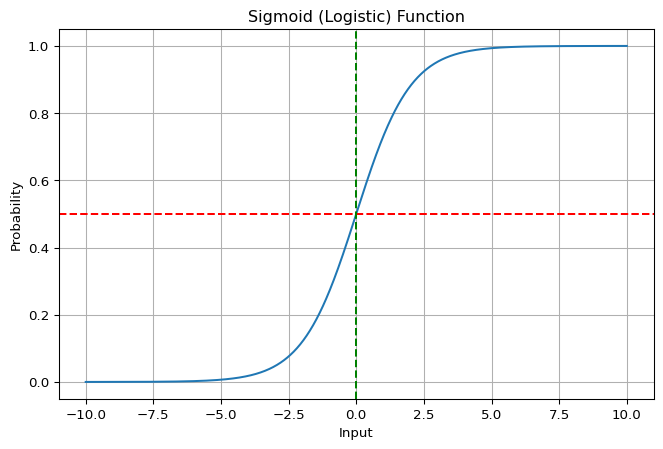
\includegraphics[keepaspectratio]{chapter4_files/figure-pdf/cell-6-output-3.png}}

\subsection{Types of Logistic
Regression}\label{types-of-logistic-regression}

\begin{enumerate}
\def\labelenumi{\arabic{enumi}.}
\tightlist
\item
  \textbf{Binary Logistic Regression}: Two possible outcomes (e.g.,
  spam/not spam)
\item
  \textbf{Multinomial Logistic Regression}: Multiple classes without
  order (e.g., predicting fruit type)
\item
  \textbf{Ordinal Logistic Regression}: Multiple classes with order
  (e.g., movie ratings)
\end{enumerate}

\subsection{Maximum Likelihood
Estimation}\label{maximum-likelihood-estimation}

Logistic regression uses Maximum Likelihood Estimation (MLE) to find the
optimal parameters. It seeks to maximize the probability of observing
the data given the parameters.

\subsection{Evaluation Metrics}\label{evaluation-metrics}

\begin{itemize}
\tightlist
\item
  \textbf{Accuracy}: Proportion of correct predictions
\item
  \textbf{Precision}: True positives / (True positives + False
  positives)
\item
  \textbf{Recall}: True positives / (True positives + False negatives)
\item
  \textbf{F1 Score}: Harmonic mean of precision and recall
\item
  \textbf{AUC-ROC}: Area under the Receiver Operating Characteristic
  curve
\end{itemize}

\subsection{Regularization}\label{regularization}

Logistic regression can benefit from regularization to prevent
overfitting: - \textbf{L1 Regularization (Lasso)}: Adds absolute value
of coefficients to loss function - \textbf{L2 Regularization (Ridge)}:
Adds squared value of coefficients to loss function

\begin{Shaded}
\begin{Highlighting}[]
\CommentTok{\# Example: Logistic Regression with Regularization}
\CommentTok{\# Comparing different regularization strengths}
\NormalTok{C\_values }\OperatorTok{=}\NormalTok{ [}\FloatTok{0.01}\NormalTok{, }\FloatTok{0.1}\NormalTok{, }\DecValTok{1}\NormalTok{, }\DecValTok{10}\NormalTok{, }\DecValTok{100}\NormalTok{]}
\NormalTok{train\_scores }\OperatorTok{=}\NormalTok{ []}
\NormalTok{test\_scores }\OperatorTok{=}\NormalTok{ []}

\ControlFlowTok{for}\NormalTok{ C }\KeywordTok{in}\NormalTok{ C\_values:}
    \CommentTok{\# C is inverse of regularization strength}
\NormalTok{    log\_reg }\OperatorTok{=}\NormalTok{ LogisticRegression(C}\OperatorTok{=}\NormalTok{C, max\_iter}\OperatorTok{=}\DecValTok{1000}\NormalTok{)}
\NormalTok{    log\_reg.fit(X\_train, y\_train)}
    
    \CommentTok{\# Score on training data}
\NormalTok{    train\_score }\OperatorTok{=}\NormalTok{ log\_reg.score(X\_train, y\_train)}
\NormalTok{    train\_scores.append(train\_score)}
    
    \CommentTok{\# Score on test data}
\NormalTok{    test\_score }\OperatorTok{=}\NormalTok{ log\_reg.score(X\_test, y\_test)}
\NormalTok{    test\_scores.append(test\_score)}

\NormalTok{plt.figure(figsize}\OperatorTok{=}\NormalTok{(}\DecValTok{10}\NormalTok{, }\DecValTok{6}\NormalTok{))}
\NormalTok{plt.semilogx(C\_values, train\_scores, label}\OperatorTok{=}\StringTok{\textquotesingle{}Training Accuracy\textquotesingle{}}\NormalTok{)}
\NormalTok{plt.semilogx(C\_values, test\_scores, label}\OperatorTok{=}\StringTok{\textquotesingle{}Testing Accuracy\textquotesingle{}}\NormalTok{)}
\NormalTok{plt.xlabel(}\StringTok{\textquotesingle{}Regularization strength (C)\textquotesingle{}}\NormalTok{)}
\NormalTok{plt.ylabel(}\StringTok{\textquotesingle{}Accuracy\textquotesingle{}}\NormalTok{)}
\NormalTok{plt.title(}\StringTok{\textquotesingle{}Effect of Regularization on Logistic Regression\textquotesingle{}}\NormalTok{)}
\NormalTok{plt.legend()}
\NormalTok{plt.grid(}\VariableTok{True}\NormalTok{)}
\NormalTok{plt.show()}
\end{Highlighting}
\end{Shaded}

\pandocbounded{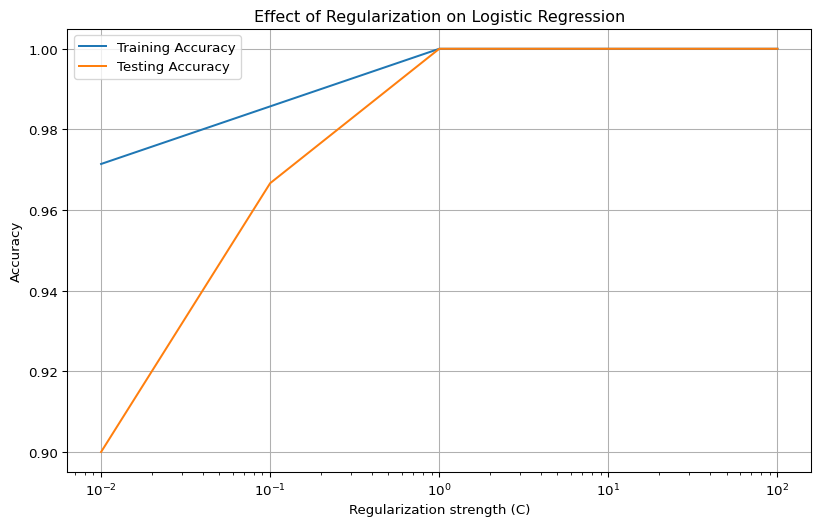
\includegraphics[keepaspectratio]{chapter4_files/figure-pdf/cell-7-output-1.png}}

\subsection{Advantages and
Disadvantages}\label{advantages-and-disadvantages-2}

\textbf{Advantages}: - Outputs probabilities - Highly interpretable
coefficients - Efficient training - Works well for linearly separable
classes - Can be extended to multi-class problems

\textbf{Disadvantages}: - Limited to linear decision boundaries -
Requires feature engineering for complex relationships - Can suffer from
complete separation issues - Sensitive to outliers and imbalanced data

\subsection{Applications}\label{applications-3}

\begin{itemize}
\tightlist
\item
  Credit scoring
\item
  Medical diagnosis
\item
  Email spam detection
\item
  Customer churn prediction
\item
  Marketing campaign effectiveness
\end{itemize}

\section{Comparison of Algorithms}\label{comparison-of-algorithms}

\begin{Shaded}
\begin{Highlighting}[]
\CommentTok{\# Generate a dataset for comparison}
\NormalTok{np.random.seed(}\DecValTok{42}\NormalTok{)}
\NormalTok{X, y }\OperatorTok{=}\NormalTok{ make\_classification(n\_samples}\OperatorTok{=}\DecValTok{1000}\NormalTok{, n\_features}\OperatorTok{=}\DecValTok{2}\NormalTok{, n\_redundant}\OperatorTok{=}\DecValTok{0}\NormalTok{, }
\NormalTok{                           n\_informative}\OperatorTok{=}\DecValTok{2}\NormalTok{, random\_state}\OperatorTok{=}\DecValTok{42}\NormalTok{, n\_clusters\_per\_class}\OperatorTok{=}\DecValTok{1}\NormalTok{)}

\CommentTok{\# Split the data}
\NormalTok{X\_train, X\_test, y\_train, y\_test }\OperatorTok{=}\NormalTok{ train\_test\_split(X, y, test\_size}\OperatorTok{=}\FloatTok{0.3}\NormalTok{, random\_state}\OperatorTok{=}\DecValTok{42}\NormalTok{)}

\CommentTok{\# Train models}
\NormalTok{knn\_model }\OperatorTok{=}\NormalTok{ KNeighborsClassifier(n\_neighbors}\OperatorTok{=}\DecValTok{5}\NormalTok{)}
\NormalTok{log\_reg\_model }\OperatorTok{=}\NormalTok{ LogisticRegression()}

\NormalTok{knn\_model.fit(X\_train, y\_train)}
\NormalTok{log\_reg\_model.fit(X\_train, y\_train)}

\CommentTok{\# Predict}
\NormalTok{knn\_pred }\OperatorTok{=}\NormalTok{ knn\_model.predict(X\_test)}
\NormalTok{log\_reg\_pred }\OperatorTok{=}\NormalTok{ log\_reg\_model.predict(X\_test)}

\CommentTok{\# Evaluate}
\NormalTok{knn\_acc }\OperatorTok{=}\NormalTok{ accuracy\_score(y\_test, knn\_pred)}
\NormalTok{log\_reg\_acc }\OperatorTok{=}\NormalTok{ accuracy\_score(y\_test, log\_reg\_pred)}

\BuiltInTok{print}\NormalTok{(}\SpecialStringTok{f"KNN Accuracy: }\SpecialCharTok{\{}\NormalTok{knn\_acc}\SpecialCharTok{:.4f\}}\SpecialStringTok{"}\NormalTok{)}
\BuiltInTok{print}\NormalTok{(}\SpecialStringTok{f"Logistic Regression Accuracy: }\SpecialCharTok{\{}\NormalTok{log\_reg\_acc}\SpecialCharTok{:.4f\}}\SpecialStringTok{"}\NormalTok{)}

\CommentTok{\# Visualize decision boundaries}
\NormalTok{fig, (ax1, ax2) }\OperatorTok{=}\NormalTok{ plt.subplots(}\DecValTok{1}\NormalTok{, }\DecValTok{2}\NormalTok{, figsize}\OperatorTok{=}\NormalTok{(}\DecValTok{15}\NormalTok{, }\DecValTok{6}\NormalTok{))}

\CommentTok{\# Create mesh grid}
\NormalTok{h }\OperatorTok{=} \FloatTok{0.02}  \CommentTok{\# step size in the mesh}
\NormalTok{x\_min, x\_max }\OperatorTok{=}\NormalTok{ X[:, }\DecValTok{0}\NormalTok{].}\BuiltInTok{min}\NormalTok{() }\OperatorTok{{-}} \DecValTok{1}\NormalTok{, X[:, }\DecValTok{0}\NormalTok{].}\BuiltInTok{max}\NormalTok{() }\OperatorTok{+} \DecValTok{1}
\NormalTok{y\_min, y\_max }\OperatorTok{=}\NormalTok{ X[:, }\DecValTok{1}\NormalTok{].}\BuiltInTok{min}\NormalTok{() }\OperatorTok{{-}} \DecValTok{1}\NormalTok{, X[:, }\DecValTok{1}\NormalTok{].}\BuiltInTok{max}\NormalTok{() }\OperatorTok{+} \DecValTok{1}
\NormalTok{xx, yy }\OperatorTok{=}\NormalTok{ np.meshgrid(np.arange(x\_min, x\_max, h), np.arange(y\_min, y\_max, h))}

\CommentTok{\# KNN decision boundary}
\NormalTok{Z }\OperatorTok{=}\NormalTok{ knn\_model.predict(np.c\_[xx.ravel(), yy.ravel()])}
\NormalTok{Z }\OperatorTok{=}\NormalTok{ Z.reshape(xx.shape)}
\NormalTok{ax1.contourf(xx, yy, Z, alpha}\OperatorTok{=}\FloatTok{0.8}\NormalTok{, cmap}\OperatorTok{=}\NormalTok{plt.cm.RdBu)}
\NormalTok{ax1.scatter(X[:, }\DecValTok{0}\NormalTok{], X[:, }\DecValTok{1}\NormalTok{], c}\OperatorTok{=}\NormalTok{y, edgecolors}\OperatorTok{=}\StringTok{\textquotesingle{}k\textquotesingle{}}\NormalTok{, cmap}\OperatorTok{=}\NormalTok{plt.cm.RdBu)}
\NormalTok{ax1.set\_title(}\SpecialStringTok{f\textquotesingle{}KNN (k=5), Accuracy: }\SpecialCharTok{\{}\NormalTok{knn\_acc}\SpecialCharTok{:.4f\}}\SpecialStringTok{\textquotesingle{}}\NormalTok{)}

\CommentTok{\# Logistic Regression decision boundary}
\NormalTok{Z }\OperatorTok{=}\NormalTok{ log\_reg\_model.predict(np.c\_[xx.ravel(), yy.ravel()])}
\NormalTok{Z }\OperatorTok{=}\NormalTok{ Z.reshape(xx.shape)}
\NormalTok{ax2.contourf(xx, yy, Z, alpha}\OperatorTok{=}\FloatTok{0.8}\NormalTok{, cmap}\OperatorTok{=}\NormalTok{plt.cm.RdBu)}
\NormalTok{ax2.scatter(X[:, }\DecValTok{0}\NormalTok{], X[:, }\DecValTok{1}\NormalTok{], c}\OperatorTok{=}\NormalTok{y, edgecolors}\OperatorTok{=}\StringTok{\textquotesingle{}k\textquotesingle{}}\NormalTok{, cmap}\OperatorTok{=}\NormalTok{plt.cm.RdBu)}
\NormalTok{ax2.set\_title(}\SpecialStringTok{f\textquotesingle{}Logistic Regression, Accuracy: }\SpecialCharTok{\{}\NormalTok{log\_reg\_acc}\SpecialCharTok{:.4f\}}\SpecialStringTok{\textquotesingle{}}\NormalTok{)}

\NormalTok{plt.tight\_layout()}
\NormalTok{plt.show()}
\end{Highlighting}
\end{Shaded}

\begin{verbatim}
KNN Accuracy: 0.9367
Logistic Regression Accuracy: 0.8833
\end{verbatim}

\pandocbounded{\includegraphics[keepaspectratio]{chapter4_files/figure-pdf/cell-8-output-2.png}}

\section{Summary}\label{summary}

This lecture covered three fundamental supervised learning algorithms:

\begin{enumerate}
\def\labelenumi{\arabic{enumi}.}
\tightlist
\item
  \textbf{K-Nearest Neighbors (KNN)}

  \begin{itemize}
  \tightlist
  \item
    Non-parametric instance-based learning
  \item
    Makes predictions based on similarity (distance metrics)
  \item
    Works for both classification and regression
  \item
    Simple but powerful for many applications
  \end{itemize}
\item
  \textbf{Linear Regression}

  \begin{itemize}
  \tightlist
  \item
    Models linear relationship between dependent and independent
    variables
  \item
    Uses least squares method to minimize errors
  \item
    Best for numeric predictions where relationships are linear
  \item
    Provides interpretable coefficients
  \end{itemize}
\item
  \textbf{Logistic Regression}

  \begin{itemize}
  \tightlist
  \item
    Despite its name, used for classification problems
  \item
    Estimates probabilities using the sigmoid function
  \item
    Outputs values between 0 and 1 (probabilities)
  \item
    Works well for binary and multi-class classification
  \end{itemize}
\end{enumerate}

\subsection{Choosing the Right
Algorithm}\label{choosing-the-right-algorithm}

\begin{itemize}
\tightlist
\item
  Use \textbf{KNN} when:

  \begin{itemize}
  \tightlist
  \item
    The decision boundary is complex
  \item
    You need a simple, interpretable model
  \item
    The dataset is small to medium sized
  \item
    Preprocessing and feature scaling are properly applied
  \end{itemize}
\item
  Use \textbf{Linear Regression} when:

  \begin{itemize}
  \tightlist
  \item
    The relationship between variables is approximately linear
  \item
    You need a continuous numerical prediction
  \item
    Interpretability of coefficients is important
  \item
    You need a baseline regression model
  \end{itemize}
\item
  Use \textbf{Logistic Regression} when:

  \begin{itemize}
  \tightlist
  \item
    You need class probabilities as output
  \item
    The decision boundary is approximately linear
  \item
    You need an interpretable model
  \item
    Feature importance is of interest
  \end{itemize}
\end{itemize}

\bookmarksetup{startatroot}

\chapter{Dimensionality Reduction
Methods}\label{dimensionality-reduction-methods}

Dimensionality reduction is a critical technique in data analysis and
machine learning that reduces the number of input variables (features)
while preserving essential information. High-dimensional datasets often
contain redundancy or noise that can be eliminated through these
methods.

\begin{figure}

\centering{

\begin{Shaded}
\begin{Highlighting}[]
\ImportTok{import}\NormalTok{ numpy }\ImportTok{as}\NormalTok{ np}
\ImportTok{import}\NormalTok{ pandas }\ImportTok{as}\NormalTok{ pd}
\ImportTok{import}\NormalTok{ matplotlib.pyplot }\ImportTok{as}\NormalTok{ plt}
\ImportTok{import}\NormalTok{ seaborn }\ImportTok{as}\NormalTok{ sns}
\ImportTok{from}\NormalTok{ sklearn.datasets }\ImportTok{import}\NormalTok{ load\_iris, fetch\_openml}
\ImportTok{from}\NormalTok{ sklearn.preprocessing }\ImportTok{import}\NormalTok{ StandardScaler}
\ImportTok{from}\NormalTok{ sklearn.decomposition }\ImportTok{import}\NormalTok{ PCA, KernelPCA, IncrementalPCA}
\ImportTok{from}\NormalTok{ sklearn.discriminant\_analysis }\ImportTok{import}\NormalTok{ LinearDiscriminantAnalysis}
\ImportTok{from}\NormalTok{ sklearn.manifold }\ImportTok{import}\NormalTok{ TSNE}
\ImportTok{import}\NormalTok{ plotly.express }\ImportTok{as}\NormalTok{ px}

\CommentTok{\# Set plotting styles}
\NormalTok{sns.set\_style(}\StringTok{"whitegrid"}\NormalTok{)}
\NormalTok{plt.rcParams[}\StringTok{\textquotesingle{}figure.figsize\textquotesingle{}}\NormalTok{] }\OperatorTok{=}\NormalTok{ (}\DecValTok{10}\NormalTok{, }\DecValTok{6}\NormalTok{)}
\end{Highlighting}
\end{Shaded}

}

\caption{\label{fig-libraries}}

\end{figure}%

\section{Why Reduce Dimensionality?}\label{why-reduce-dimensionality}

The primary goals of dimensionality reduction include:

\begin{enumerate}
\def\labelenumi{\arabic{enumi}.}
\tightlist
\item
  \textbf{Reducing overfitting} by eliminating noise and redundant
  features
\item
  \textbf{Improving computational efficiency} for faster, less expensive
  algorithms
\item
  \textbf{Enabling data visualization} by mapping to 2D or 3D spaces
\item
  \textbf{Removing noise} to focus on meaningful patterns
\end{enumerate}

\section{Dataset Example: Iris}\label{dataset-example-iris}

Let's load and examine the Iris dataset, which we'll use throughout this
document:

\begin{Shaded}
\begin{Highlighting}[]
\CommentTok{\# Load the Iris dataset}
\NormalTok{iris }\OperatorTok{=}\NormalTok{ load\_iris()}
\NormalTok{X }\OperatorTok{=}\NormalTok{ iris.data}
\NormalTok{y }\OperatorTok{=}\NormalTok{ iris.target}
\NormalTok{feature\_names }\OperatorTok{=}\NormalTok{ iris.feature\_names}
\NormalTok{target\_names }\OperatorTok{=}\NormalTok{ iris.target\_names}

\CommentTok{\# Create a DataFrame for easier manipulation}
\NormalTok{iris\_df }\OperatorTok{=}\NormalTok{ pd.DataFrame(X, columns}\OperatorTok{=}\NormalTok{feature\_names)}
\NormalTok{iris\_df[}\StringTok{\textquotesingle{}species\textquotesingle{}}\NormalTok{] }\OperatorTok{=}\NormalTok{ [target\_names[i] }\ControlFlowTok{for}\NormalTok{ i }\KeywordTok{in}\NormalTok{ y]}

\CommentTok{\# Display dataset information}
\BuiltInTok{print}\NormalTok{(}\SpecialStringTok{f"Dataset shape: }\SpecialCharTok{\{}\NormalTok{X}\SpecialCharTok{.}\NormalTok{shape}\SpecialCharTok{\}}\SpecialStringTok{"}\NormalTok{)}
\BuiltInTok{print}\NormalTok{(}\SpecialStringTok{f"Features: }\SpecialCharTok{\{}\NormalTok{feature\_names}\SpecialCharTok{\}}\SpecialStringTok{"}\NormalTok{)}
\BuiltInTok{print}\NormalTok{(}\SpecialStringTok{f"Number of samples per class: }\SpecialCharTok{\{}\NormalTok{np}\SpecialCharTok{.}\NormalTok{bincount(y)}\SpecialCharTok{\}}\SpecialStringTok{"}\NormalTok{)}

\CommentTok{\# Preview the dataset}
\NormalTok{iris\_df.head()}
\end{Highlighting}
\end{Shaded}

\begin{verbatim}
Dataset shape: (150, 4)
Features: ['sepal length (cm)', 'sepal width (cm)', 'petal length (cm)', 'petal width (cm)']
Number of samples per class: [50 50 50]
\end{verbatim}

\phantomsection\label{fig-iris-data}
\begin{longtable}[]{@{}llllll@{}}
\toprule\noalign{}
& sepal length (cm) & sepal width (cm) & petal length (cm) & petal width
(cm) & species \\
\midrule\noalign{}
\endhead
\bottomrule\noalign{}
\endlastfoot
0 & 5.1 & 3.5 & 1.4 & 0.2 & setosa \\
1 & 4.9 & 3.0 & 1.4 & 0.2 & setosa \\
2 & 4.7 & 3.2 & 1.3 & 0.2 & setosa \\
3 & 4.6 & 3.1 & 1.5 & 0.2 & setosa \\
4 & 5.0 & 3.6 & 1.4 & 0.2 & setosa \\
\end{longtable}

\section{Approaches to Dimensionality
Reduction}\label{approaches-to-dimensionality-reduction}

Dimensionality reduction methods fall into two main categories:

\subsection{Unsupervised Methods}\label{unsupervised-methods}

These techniques don't require labeled data and find lower-dimensional
representations based solely on the intrinsic structure of features.

\subsubsection{Principal Component Analysis
(PCA)}\label{principal-component-analysis-pca}

PCA identifies directions (principal components) where data varies the
most and projects data onto this lower-dimensional space.

\begin{Shaded}
\begin{Highlighting}[]
\CommentTok{\# Standardize the data}
\NormalTok{scaler }\OperatorTok{=}\NormalTok{ StandardScaler()}
\NormalTok{X\_scaled }\OperatorTok{=}\NormalTok{ scaler.fit\_transform(X)}

\CommentTok{\# Apply PCA}
\NormalTok{pca }\OperatorTok{=}\NormalTok{ PCA()}
\NormalTok{X\_pca }\OperatorTok{=}\NormalTok{ pca.fit\_transform(X\_scaled)}

\CommentTok{\# Plot explained variance}
\NormalTok{plt.figure(figsize}\OperatorTok{=}\NormalTok{(}\DecValTok{10}\NormalTok{, }\DecValTok{6}\NormalTok{))}
\NormalTok{plt.bar(}\BuiltInTok{range}\NormalTok{(}\DecValTok{1}\NormalTok{, }\BuiltInTok{len}\NormalTok{(pca.explained\_variance\_ratio\_) }\OperatorTok{+} \DecValTok{1}\NormalTok{), pca.explained\_variance\_ratio\_)}
\NormalTok{plt.plot(}\BuiltInTok{range}\NormalTok{(}\DecValTok{1}\NormalTok{, }\BuiltInTok{len}\NormalTok{(pca.explained\_variance\_ratio\_) }\OperatorTok{+} \DecValTok{1}\NormalTok{), }
\NormalTok{         np.cumsum(pca.explained\_variance\_ratio\_), }\StringTok{\textquotesingle{}r{-}o\textquotesingle{}}\NormalTok{)}
\NormalTok{plt.xlabel(}\StringTok{\textquotesingle{}Principal Component\textquotesingle{}}\NormalTok{)}
\NormalTok{plt.ylabel(}\StringTok{\textquotesingle{}Explained Variance Ratio / Cumulative\textquotesingle{}}\NormalTok{)}
\NormalTok{plt.xticks(}\BuiltInTok{range}\NormalTok{(}\DecValTok{1}\NormalTok{, }\BuiltInTok{len}\NormalTok{(pca.explained\_variance\_ratio\_) }\OperatorTok{+} \DecValTok{1}\NormalTok{))}
\NormalTok{plt.title(}\StringTok{\textquotesingle{}Explained Variance by Principal Components\textquotesingle{}}\NormalTok{)}
\NormalTok{plt.grid(}\VariableTok{True}\NormalTok{)}
\NormalTok{plt.show()}

\CommentTok{\# Print variance explained}
\BuiltInTok{print}\NormalTok{(}\SpecialStringTok{f"Variance explained by each component: }\SpecialCharTok{\{}\NormalTok{pca}\SpecialCharTok{.}\NormalTok{explained\_variance\_ratio\_}\SpecialCharTok{\}}\SpecialStringTok{"}\NormalTok{)}
\BuiltInTok{print}\NormalTok{(}\SpecialStringTok{f"Cumulative variance explained: }\SpecialCharTok{\{}\NormalTok{np}\SpecialCharTok{.}\NormalTok{cumsum(pca.explained\_variance\_ratio\_)}\SpecialCharTok{\}}\SpecialStringTok{"}\NormalTok{)}

\CommentTok{\# Visualization in 2D}
\NormalTok{plt.figure(figsize}\OperatorTok{=}\NormalTok{(}\DecValTok{10}\NormalTok{, }\DecValTok{8}\NormalTok{))}
\NormalTok{colors }\OperatorTok{=}\NormalTok{ [}\StringTok{\textquotesingle{}navy\textquotesingle{}}\NormalTok{, }\StringTok{\textquotesingle{}turquoise\textquotesingle{}}\NormalTok{, }\StringTok{\textquotesingle{}darkorange\textquotesingle{}}\NormalTok{]}
\ControlFlowTok{for}\NormalTok{ i, c, label }\KeywordTok{in} \BuiltInTok{zip}\NormalTok{(}\BuiltInTok{range}\NormalTok{(}\DecValTok{3}\NormalTok{), colors, target\_names):}
\NormalTok{    plt.scatter(X\_pca[y }\OperatorTok{==}\NormalTok{ i, }\DecValTok{0}\NormalTok{], X\_pca[y }\OperatorTok{==}\NormalTok{ i, }\DecValTok{1}\NormalTok{], c}\OperatorTok{=}\NormalTok{c, label}\OperatorTok{=}\NormalTok{label)}
\NormalTok{plt.xlabel(}\StringTok{\textquotesingle{}First Principal Component\textquotesingle{}}\NormalTok{)}
\NormalTok{plt.ylabel(}\StringTok{\textquotesingle{}Second Principal Component\textquotesingle{}}\NormalTok{)}
\NormalTok{plt.title(}\StringTok{\textquotesingle{}PCA of Iris Dataset\textquotesingle{}}\NormalTok{)}
\NormalTok{plt.legend()}
\NormalTok{plt.grid(}\VariableTok{True}\NormalTok{)}
\NormalTok{plt.show()}
\end{Highlighting}
\end{Shaded}

\begin{verbatim}
Variance explained by each component: [0.72962445 0.22850762 0.03668922 0.00517871]
Cumulative variance explained: [0.72962445 0.95813207 0.99482129 1.        ]
\end{verbatim}

\begin{figure}[H]

\centering{

\centering{

\pandocbounded{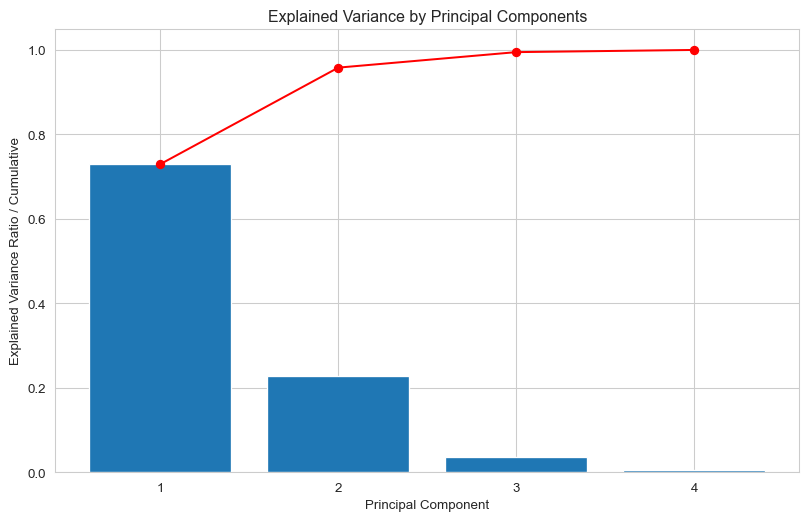
\includegraphics[keepaspectratio]{chapter5_files/figure-pdf/fig-pca-iris-output-1.png}}

}

\subcaption{\label{fig-pca-iris-1}PCA visualization of the Iris dataset}

\centering{

\pandocbounded{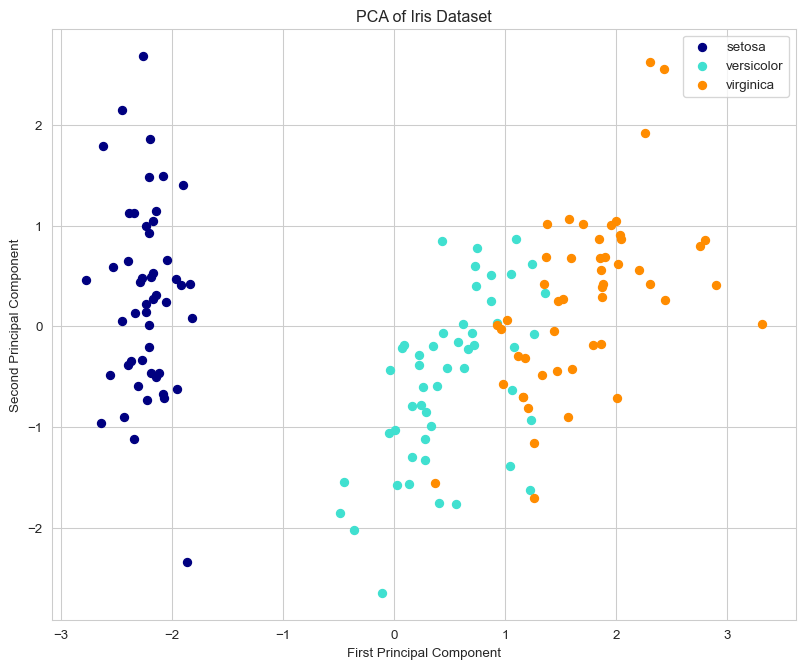
\includegraphics[keepaspectratio]{chapter5_files/figure-pdf/fig-pca-iris-output-3.png}}

}

\subcaption{\label{fig-pca-iris-2}}

}

\caption{\label{fig-pca-iris}}

\end{figure}%

\paragraph{Key Concepts of PCA}\label{key-concepts-of-pca}

\begin{enumerate}
\def\labelenumi{\arabic{enumi}.}
\tightlist
\item
  \textbf{Variance Maximization}: Captures directions with maximum
  variance
\item
  \textbf{Linear Combinations}: Each PC is a weighted sum of original
  features
\item
  \textbf{Uncorrelated Components}: PCs are orthogonal to each other
\item
  \textbf{Coordinate Transformation}: Rotates data into a new coordinate
  system
\end{enumerate}

Let's explore the relationship between original features and principal
components:

\begin{Shaded}
\begin{Highlighting}[]
\CommentTok{\# Display the component loadings}
\NormalTok{loadings }\OperatorTok{=}\NormalTok{ pd.DataFrame(}
\NormalTok{    pca.components\_.T,}
\NormalTok{    columns}\OperatorTok{=}\NormalTok{[}\SpecialStringTok{f\textquotesingle{}PC}\SpecialCharTok{\{}\NormalTok{i}\OperatorTok{+}\DecValTok{1}\SpecialCharTok{\}}\SpecialStringTok{\textquotesingle{}} \ControlFlowTok{for}\NormalTok{ i }\KeywordTok{in} \BuiltInTok{range}\NormalTok{(pca.components\_.shape[}\DecValTok{0}\NormalTok{])],}
\NormalTok{    index}\OperatorTok{=}\NormalTok{feature\_names}
\NormalTok{)}

\CommentTok{\# Visualize the loadings}
\NormalTok{plt.figure(figsize}\OperatorTok{=}\NormalTok{(}\DecValTok{10}\NormalTok{, }\DecValTok{6}\NormalTok{))}
\NormalTok{sns.heatmap(loadings, annot}\OperatorTok{=}\VariableTok{True}\NormalTok{, cmap}\OperatorTok{=}\StringTok{\textquotesingle{}coolwarm\textquotesingle{}}\NormalTok{, fmt}\OperatorTok{=}\StringTok{\textquotesingle{}.3f\textquotesingle{}}\NormalTok{)}
\NormalTok{plt.title(}\StringTok{\textquotesingle{}PCA Component Loadings\textquotesingle{}}\NormalTok{)}
\NormalTok{plt.tight\_layout()}
\NormalTok{plt.show()}

\CommentTok{\# Determine optimal number of components for 95\% variance}
\NormalTok{cumsum }\OperatorTok{=}\NormalTok{ np.cumsum(pca.explained\_variance\_ratio\_)}
\NormalTok{d }\OperatorTok{=}\NormalTok{ np.argmax(cumsum }\OperatorTok{\textgreater{}=} \FloatTok{0.95}\NormalTok{) }\OperatorTok{+} \DecValTok{1}
\BuiltInTok{print}\NormalTok{(}\SpecialStringTok{f"Number of components needed for 95\% variance: }\SpecialCharTok{\{}\NormalTok{d}\SpecialCharTok{\}}\SpecialStringTok{"}\NormalTok{)}
\end{Highlighting}
\end{Shaded}

\begin{figure}[H]

\centering{

\pandocbounded{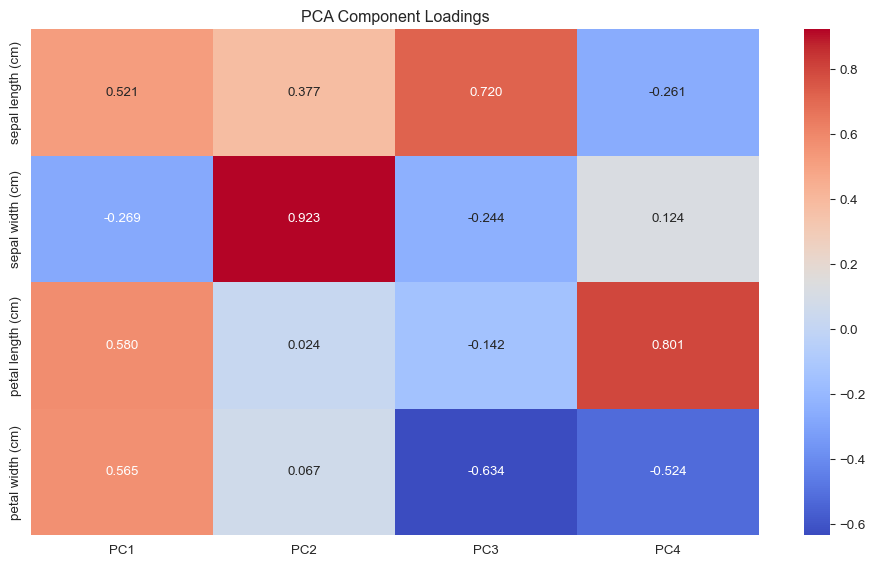
\includegraphics[keepaspectratio]{chapter5_files/figure-pdf/fig-pca-components-output-1.png}}

}

\caption{\label{fig-pca-components}PCA components and their relationship
to original features}

\end{figure}%

\begin{verbatim}
Number of components needed for 95% variance: 2
\end{verbatim}

\subsubsection{Other Unsupervised
Methods}\label{other-unsupervised-methods}

\begin{itemize}
\tightlist
\item
  \textbf{Independent Component Analysis (ICA)}: Focuses on statistical
  independence of components
\item
  \textbf{Non-negative Matrix Factorization (NMF)}: Factorizes data into
  non-negative matrices
\end{itemize}

\subsection{Supervised Methods}\label{supervised-methods}

These techniques consider class labels during dimensionality reduction
to better preserve class separability.

\subsubsection{Linear Discriminant Analysis
(LDA)}\label{linear-discriminant-analysis-lda}

LDA maximizes class separation by projecting data onto a
lower-dimensional space:

\begin{Shaded}
\begin{Highlighting}[]
\CommentTok{\# Apply LDA}
\NormalTok{lda }\OperatorTok{=}\NormalTok{ LinearDiscriminantAnalysis(n\_components}\OperatorTok{=}\DecValTok{2}\NormalTok{)}
\NormalTok{X\_lda }\OperatorTok{=}\NormalTok{ lda.fit\_transform(X\_scaled, y)}

\CommentTok{\# Visualization in 2D}
\NormalTok{plt.figure(figsize}\OperatorTok{=}\NormalTok{(}\DecValTok{10}\NormalTok{, }\DecValTok{8}\NormalTok{))}
\ControlFlowTok{for}\NormalTok{ i, c, label }\KeywordTok{in} \BuiltInTok{zip}\NormalTok{(}\BuiltInTok{range}\NormalTok{(}\DecValTok{3}\NormalTok{), colors, target\_names):}
\NormalTok{    plt.scatter(X\_lda[y }\OperatorTok{==}\NormalTok{ i, }\DecValTok{0}\NormalTok{], X\_lda[y }\OperatorTok{==}\NormalTok{ i, }\DecValTok{1}\NormalTok{], c}\OperatorTok{=}\NormalTok{c, label}\OperatorTok{=}\NormalTok{label)}
\NormalTok{plt.xlabel(}\StringTok{\textquotesingle{}First LDA Component\textquotesingle{}}\NormalTok{)}
\NormalTok{plt.ylabel(}\StringTok{\textquotesingle{}Second LDA Component\textquotesingle{}}\NormalTok{)}
\NormalTok{plt.title(}\StringTok{\textquotesingle{}LDA of Iris Dataset\textquotesingle{}}\NormalTok{)}
\NormalTok{plt.legend()}
\NormalTok{plt.grid(}\VariableTok{True}\NormalTok{)}
\NormalTok{plt.show()}

\CommentTok{\# Check explained variance ratio}
\BuiltInTok{print}\NormalTok{(}\SpecialStringTok{f"Explained variance ratio: }\SpecialCharTok{\{}\NormalTok{lda}\SpecialCharTok{.}\NormalTok{explained\_variance\_ratio\_}\SpecialCharTok{\}}\SpecialStringTok{"}\NormalTok{)}
\end{Highlighting}
\end{Shaded}

\begin{figure}[H]

\centering{

\pandocbounded{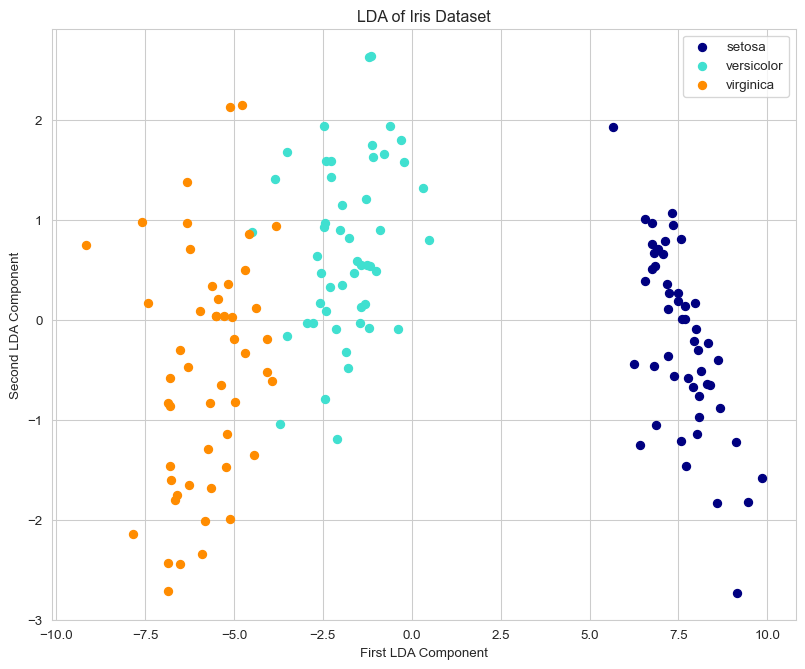
\includegraphics[keepaspectratio]{chapter5_files/figure-pdf/fig-lda-iris-output-1.png}}

}

\caption{\label{fig-lda-iris}LDA visualization of the Iris dataset}

\end{figure}%

\begin{verbatim}
Explained variance ratio: [0.9912126 0.0087874]
\end{verbatim}

\section{Advanced PCA
Implementations}\label{advanced-pca-implementations}

\subsection{Kernel PCA}\label{kernel-pca}

When data is not linearly separable, Kernel PCA can be more effective:

\begin{Shaded}
\begin{Highlighting}[]
\CommentTok{\# Apply Kernel PCA with different kernels}
\NormalTok{kernels }\OperatorTok{=}\NormalTok{ [}\StringTok{\textquotesingle{}linear\textquotesingle{}}\NormalTok{, }\StringTok{\textquotesingle{}poly\textquotesingle{}}\NormalTok{, }\StringTok{\textquotesingle{}rbf\textquotesingle{}}\NormalTok{]}
\NormalTok{fig, axes }\OperatorTok{=}\NormalTok{ plt.subplots(}\DecValTok{1}\NormalTok{, }\BuiltInTok{len}\NormalTok{(kernels), figsize}\OperatorTok{=}\NormalTok{(}\DecValTok{18}\NormalTok{, }\DecValTok{5}\NormalTok{))}

\ControlFlowTok{for}\NormalTok{ i, kernel }\KeywordTok{in} \BuiltInTok{enumerate}\NormalTok{(kernels):}
\NormalTok{    kpca }\OperatorTok{=}\NormalTok{ KernelPCA(n\_components}\OperatorTok{=}\DecValTok{2}\NormalTok{, kernel}\OperatorTok{=}\NormalTok{kernel)}
\NormalTok{    X\_kpca }\OperatorTok{=}\NormalTok{ kpca.fit\_transform(X\_scaled)}
    
    \ControlFlowTok{for}\NormalTok{ j, c, label }\KeywordTok{in} \BuiltInTok{zip}\NormalTok{(}\BuiltInTok{range}\NormalTok{(}\DecValTok{3}\NormalTok{), colors, target\_names):}
\NormalTok{        axes[i].scatter(X\_kpca[y }\OperatorTok{==}\NormalTok{ j, }\DecValTok{0}\NormalTok{], X\_kpca[y }\OperatorTok{==}\NormalTok{ j, }\DecValTok{1}\NormalTok{], c}\OperatorTok{=}\NormalTok{c, label}\OperatorTok{=}\NormalTok{label)}
    
\NormalTok{    axes[i].set\_xlabel(}\StringTok{\textquotesingle{}First Component\textquotesingle{}}\NormalTok{)}
\NormalTok{    axes[i].set\_ylabel(}\StringTok{\textquotesingle{}Second Component\textquotesingle{}}\NormalTok{)}
\NormalTok{    axes[i].set\_title(}\SpecialStringTok{f\textquotesingle{}Kernel PCA (}\SpecialCharTok{\{}\NormalTok{kernel}\SpecialCharTok{\}}\SpecialStringTok{)\textquotesingle{}}\NormalTok{)}
\NormalTok{    axes[i].legend()}
\NormalTok{    axes[i].grid(}\VariableTok{True}\NormalTok{)}

\NormalTok{plt.tight\_layout()}
\NormalTok{plt.show()}
\end{Highlighting}
\end{Shaded}

\begin{figure}[H]

\centering{

\pandocbounded{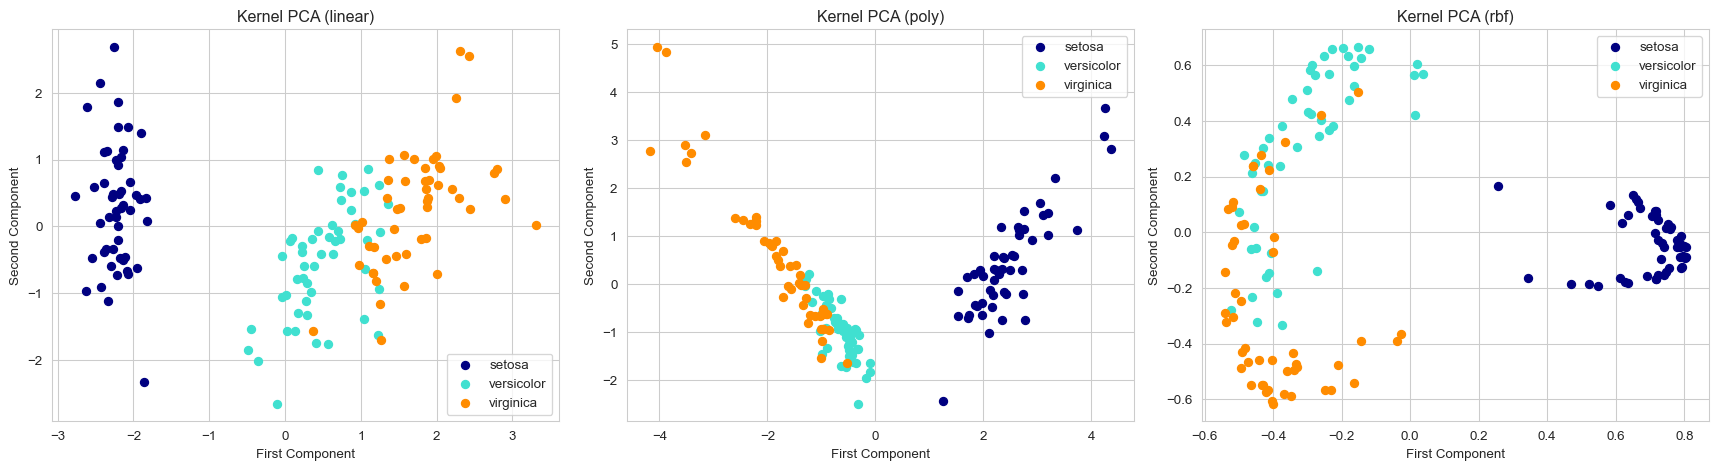
\includegraphics[keepaspectratio]{chapter5_files/figure-pdf/fig-kernel-pca-output-1.png}}

}

\caption{\label{fig-kernel-pca}Comparison of PCA and Kernel PCA}

\end{figure}%

\subsection{Incremental PCA}\label{incremental-pca}

For larger datasets, Incremental PCA processes data in batches:

\begin{Shaded}
\begin{Highlighting}[]
\CommentTok{\# Simulate a larger dataset by repeating Iris}
\NormalTok{X\_large }\OperatorTok{=}\NormalTok{ np.vstack([X\_scaled] }\OperatorTok{*} \DecValTok{10}\NormalTok{)}
\NormalTok{y\_large }\OperatorTok{=}\NormalTok{ np.hstack([y] }\OperatorTok{*} \DecValTok{10}\NormalTok{)}

\CommentTok{\# Apply Incremental PCA}
\NormalTok{n\_batches }\OperatorTok{=} \DecValTok{5}
\NormalTok{batch\_size }\OperatorTok{=}\NormalTok{ X\_large.shape[}\DecValTok{0}\NormalTok{] }\OperatorTok{//}\NormalTok{ n\_batches}

\NormalTok{ipca }\OperatorTok{=}\NormalTok{ IncrementalPCA(n\_components}\OperatorTok{=}\DecValTok{2}\NormalTok{)}
\ControlFlowTok{for}\NormalTok{ i }\KeywordTok{in} \BuiltInTok{range}\NormalTok{(n\_batches):}
\NormalTok{    start }\OperatorTok{=}\NormalTok{ i }\OperatorTok{*}\NormalTok{ batch\_size}
\NormalTok{    end }\OperatorTok{=} \BuiltInTok{min}\NormalTok{((i }\OperatorTok{+} \DecValTok{1}\NormalTok{) }\OperatorTok{*}\NormalTok{ batch\_size, X\_large.shape[}\DecValTok{0}\NormalTok{])}
\NormalTok{    ipca.partial\_fit(X\_large[start:end])}

\NormalTok{X\_ipca }\OperatorTok{=}\NormalTok{ ipca.transform(X\_large)}

\CommentTok{\# Compare with standard PCA}
\NormalTok{pca }\OperatorTok{=}\NormalTok{ PCA(n\_components}\OperatorTok{=}\DecValTok{2}\NormalTok{)}
\NormalTok{X\_pca\_large }\OperatorTok{=}\NormalTok{ pca.fit\_transform(X\_large)}

\CommentTok{\# Visualize both}
\NormalTok{fig, axes }\OperatorTok{=}\NormalTok{ plt.subplots(}\DecValTok{1}\NormalTok{, }\DecValTok{2}\NormalTok{, figsize}\OperatorTok{=}\NormalTok{(}\DecValTok{15}\NormalTok{, }\DecValTok{6}\NormalTok{))}

\CommentTok{\# Plot IPCA}
\ControlFlowTok{for}\NormalTok{ i, c, label }\KeywordTok{in} \BuiltInTok{zip}\NormalTok{(}\BuiltInTok{range}\NormalTok{(}\DecValTok{3}\NormalTok{), colors, target\_names):}
\NormalTok{    axes[}\DecValTok{0}\NormalTok{].scatter(X\_ipca[y\_large }\OperatorTok{==}\NormalTok{ i, }\DecValTok{0}\NormalTok{], X\_ipca[y\_large }\OperatorTok{==}\NormalTok{ i, }\DecValTok{1}\NormalTok{], c}\OperatorTok{=}\NormalTok{c, label}\OperatorTok{=}\NormalTok{label, alpha}\OperatorTok{=}\FloatTok{0.5}\NormalTok{)}
\NormalTok{axes[}\DecValTok{0}\NormalTok{].set\_title(}\StringTok{\textquotesingle{}Incremental PCA\textquotesingle{}}\NormalTok{)}
\NormalTok{axes[}\DecValTok{0}\NormalTok{].legend()}
\NormalTok{axes[}\DecValTok{0}\NormalTok{].grid(}\VariableTok{True}\NormalTok{)}

\CommentTok{\# Plot standard PCA}
\ControlFlowTok{for}\NormalTok{ i, c, label }\KeywordTok{in} \BuiltInTok{zip}\NormalTok{(}\BuiltInTok{range}\NormalTok{(}\DecValTok{3}\NormalTok{), colors, target\_names):}
\NormalTok{    axes[}\DecValTok{1}\NormalTok{].scatter(X\_pca\_large[y\_large }\OperatorTok{==}\NormalTok{ i, }\DecValTok{0}\NormalTok{], X\_pca\_large[y\_large }\OperatorTok{==}\NormalTok{ i, }\DecValTok{1}\NormalTok{], c}\OperatorTok{=}\NormalTok{c, label}\OperatorTok{=}\NormalTok{label, alpha}\OperatorTok{=}\FloatTok{0.5}\NormalTok{)}
\NormalTok{axes[}\DecValTok{1}\NormalTok{].set\_title(}\StringTok{\textquotesingle{}Standard PCA\textquotesingle{}}\NormalTok{)}
\NormalTok{axes[}\DecValTok{1}\NormalTok{].legend()}
\NormalTok{axes[}\DecValTok{1}\NormalTok{].grid(}\VariableTok{True}\NormalTok{)}

\NormalTok{plt.tight\_layout()}
\NormalTok{plt.show()}

\CommentTok{\# Compare explained variance}
\BuiltInTok{print}\NormalTok{(}\SpecialStringTok{f"IPCA explained variance: }\SpecialCharTok{\{}\NormalTok{ipca}\SpecialCharTok{.}\NormalTok{explained\_variance\_ratio\_}\SpecialCharTok{\}}\SpecialStringTok{"}\NormalTok{)}
\BuiltInTok{print}\NormalTok{(}\SpecialStringTok{f"PCA explained variance: }\SpecialCharTok{\{}\NormalTok{pca}\SpecialCharTok{.}\NormalTok{explained\_variance\_ratio\_}\SpecialCharTok{\}}\SpecialStringTok{"}\NormalTok{)}
\end{Highlighting}
\end{Shaded}

\begin{figure}[H]

\centering{

\pandocbounded{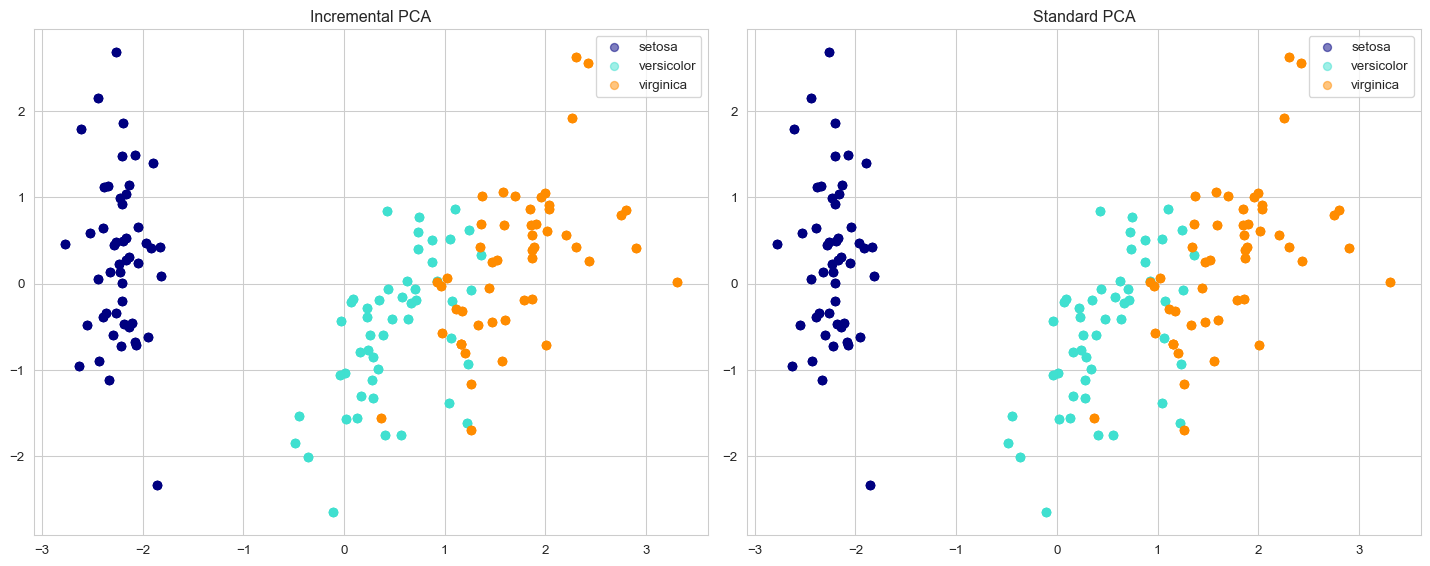
\includegraphics[keepaspectratio]{chapter5_files/figure-pdf/fig-incremental-pca-output-1.png}}

}

\caption{\label{fig-incremental-pca}}

\end{figure}%

\begin{verbatim}
IPCA explained variance: [0.72962445 0.22850762]
PCA explained variance: [0.72962445 0.22850762]
\end{verbatim}

\section{Visualizing High-Dimensional Data with
t-SNE}\label{visualizing-high-dimensional-data-with-t-sne}

t-SNE is particularly effective for visualizing high-dimensional data:

\begin{Shaded}
\begin{Highlighting}[]
\CommentTok{\# Apply t{-}SNE}
\NormalTok{tsne }\OperatorTok{=}\NormalTok{ TSNE(n\_components}\OperatorTok{=}\DecValTok{2}\NormalTok{, random\_state}\OperatorTok{=}\DecValTok{42}\NormalTok{)}
\NormalTok{X\_tsne }\OperatorTok{=}\NormalTok{ tsne.fit\_transform(X\_scaled)}

\CommentTok{\# Create visualization}
\NormalTok{plt.figure(figsize}\OperatorTok{=}\NormalTok{(}\DecValTok{10}\NormalTok{, }\DecValTok{8}\NormalTok{))}
\ControlFlowTok{for}\NormalTok{ i, c, label }\KeywordTok{in} \BuiltInTok{zip}\NormalTok{(}\BuiltInTok{range}\NormalTok{(}\DecValTok{3}\NormalTok{), colors, target\_names):}
\NormalTok{    plt.scatter(X\_tsne[y }\OperatorTok{==}\NormalTok{ i, }\DecValTok{0}\NormalTok{], X\_tsne[y }\OperatorTok{==}\NormalTok{ i, }\DecValTok{1}\NormalTok{], c}\OperatorTok{=}\NormalTok{c, label}\OperatorTok{=}\NormalTok{label)}
\NormalTok{plt.title(}\StringTok{\textquotesingle{}t{-}SNE of Iris Dataset\textquotesingle{}}\NormalTok{)}
\NormalTok{plt.legend()}
\NormalTok{plt.grid(}\VariableTok{True}\NormalTok{)}
\NormalTok{plt.show()}
\end{Highlighting}
\end{Shaded}

\begin{figure}[H]

\centering{

\pandocbounded{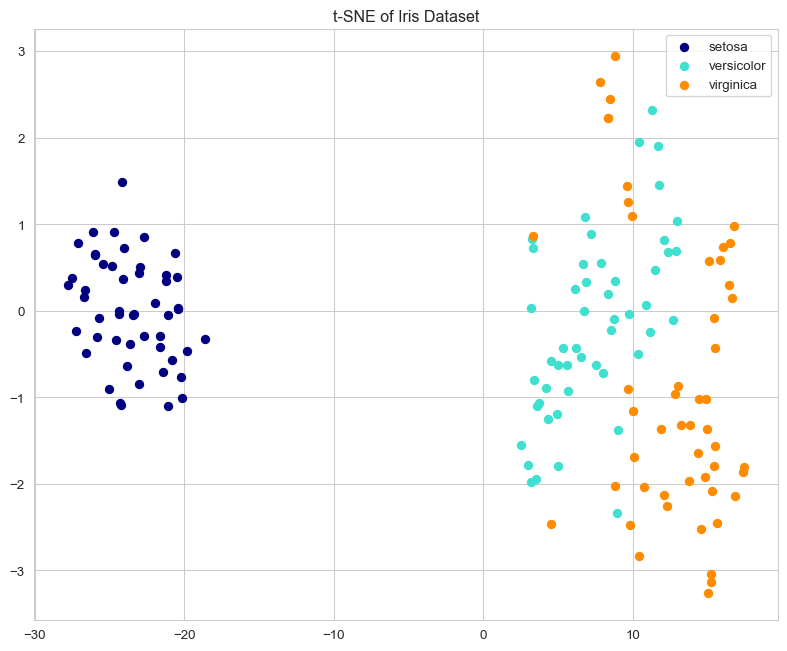
\includegraphics[keepaspectratio]{chapter5_files/figure-pdf/fig-tsne-output-1.png}}

}

\caption{\label{fig-tsne}t-SNE visualization of the Iris dataset}

\end{figure}%

\section{Real-World Application: MNIST
Dataset}\label{real-world-application-mnist-dataset}

Let's apply dimensionality reduction to a larger, more complex dataset:

\begin{figure}

\centering{

\begin{Shaded}
\begin{Highlighting}[]
\CommentTok{\# Load a subset of MNIST for demonstration}
\NormalTok{mnist }\OperatorTok{=}\NormalTok{ fetch\_openml(}\StringTok{\textquotesingle{}mnist\_784\textquotesingle{}}\NormalTok{, version}\OperatorTok{=}\DecValTok{1}\NormalTok{, as\_frame}\OperatorTok{=}\VariableTok{False}\NormalTok{, parser}\OperatorTok{=}\StringTok{\textquotesingle{}auto\textquotesingle{}}\NormalTok{)}
\NormalTok{X\_mnist }\OperatorTok{=}\NormalTok{ mnist.data[:}\DecValTok{2000}\NormalTok{]}
\NormalTok{y\_mnist }\OperatorTok{=}\NormalTok{ mnist.target[:}\DecValTok{2000}\NormalTok{].astype(}\BuiltInTok{int}\NormalTok{)}

\CommentTok{\# Standardize the data}
\NormalTok{scaler }\OperatorTok{=}\NormalTok{ StandardScaler()}
\NormalTok{X\_mnist\_scaled }\OperatorTok{=}\NormalTok{ scaler.fit\_transform(X\_mnist)}

\CommentTok{\# Apply PCA}
\NormalTok{pca\_mnist }\OperatorTok{=}\NormalTok{ PCA(n\_components}\OperatorTok{=}\DecValTok{50}\NormalTok{)  }\CommentTok{\# Reduce from 784 to 50 dimensions}
\NormalTok{X\_mnist\_pca }\OperatorTok{=}\NormalTok{ pca\_mnist.fit\_transform(X\_mnist\_scaled)}

\CommentTok{\# Plot explained variance}
\NormalTok{plt.figure(figsize}\OperatorTok{=}\NormalTok{(}\DecValTok{10}\NormalTok{, }\DecValTok{6}\NormalTok{))}
\NormalTok{plt.plot(np.cumsum(pca\_mnist.explained\_variance\_ratio\_))}
\NormalTok{plt.xlabel(}\StringTok{\textquotesingle{}Number of Components\textquotesingle{}}\NormalTok{)}
\NormalTok{plt.ylabel(}\StringTok{\textquotesingle{}Cumulative Explained Variance\textquotesingle{}}\NormalTok{)}
\NormalTok{plt.title(}\StringTok{\textquotesingle{}Explained Variance vs. Number of PCA Components (MNIST)\textquotesingle{}}\NormalTok{)}
\NormalTok{plt.grid(}\VariableTok{True}\NormalTok{)}
\NormalTok{plt.show()}

\CommentTok{\# Check how many components needed for 95\% variance}
\NormalTok{cumsum }\OperatorTok{=}\NormalTok{ np.cumsum(pca\_mnist.explained\_variance\_ratio\_)}
\NormalTok{d }\OperatorTok{=}\NormalTok{ np.argmax(cumsum }\OperatorTok{\textgreater{}=} \FloatTok{0.95}\NormalTok{) }\OperatorTok{+} \DecValTok{1}
\BuiltInTok{print}\NormalTok{(}\SpecialStringTok{f"Number of components needed for 95\% variance: }\SpecialCharTok{\{}\NormalTok{d}\SpecialCharTok{\}}\SpecialStringTok{"}\NormalTok{)}

\CommentTok{\# Visualize first two components}
\NormalTok{plt.figure(figsize}\OperatorTok{=}\NormalTok{(}\DecValTok{10}\NormalTok{, }\DecValTok{8}\NormalTok{))}
\ControlFlowTok{for}\NormalTok{ i }\KeywordTok{in} \BuiltInTok{range}\NormalTok{(}\DecValTok{10}\NormalTok{):}
\NormalTok{    plt.scatter(X\_mnist\_pca[y\_mnist }\OperatorTok{==}\NormalTok{ i, }\DecValTok{0}\NormalTok{], X\_mnist\_pca[y\_mnist }\OperatorTok{==}\NormalTok{ i, }\DecValTok{1}\NormalTok{], label}\OperatorTok{=}\BuiltInTok{str}\NormalTok{(i), alpha}\OperatorTok{=}\FloatTok{0.6}\NormalTok{)}
\NormalTok{plt.legend()}
\NormalTok{plt.title(}\StringTok{\textquotesingle{}PCA of MNIST Dataset (First 2 Components)\textquotesingle{}}\NormalTok{)}
\NormalTok{plt.grid(}\VariableTok{True}\NormalTok{)}
\NormalTok{plt.show()}

\CommentTok{\# Visualize some original vs. reconstructed images}
\NormalTok{n\_row, n\_col }\OperatorTok{=} \DecValTok{2}\NormalTok{, }\DecValTok{5}
\NormalTok{fig, axes }\OperatorTok{=}\NormalTok{ plt.subplots(n\_row, n\_col, figsize}\OperatorTok{=}\NormalTok{(}\DecValTok{15}\NormalTok{, }\DecValTok{6}\NormalTok{))}

\CommentTok{\# Reconstruct images from PCA components}
\NormalTok{X\_mnist\_reconstructed }\OperatorTok{=}\NormalTok{ pca\_mnist.inverse\_transform(X\_mnist\_pca)}
\NormalTok{X\_mnist\_reconstructed }\OperatorTok{=}\NormalTok{ scaler.inverse\_transform(X\_mnist\_reconstructed)}

\ControlFlowTok{for}\NormalTok{ i }\KeywordTok{in} \BuiltInTok{range}\NormalTok{(n\_row):}
    \ControlFlowTok{for}\NormalTok{ j }\KeywordTok{in} \BuiltInTok{range}\NormalTok{(n\_col):}
\NormalTok{        idx }\OperatorTok{=}\NormalTok{ i }\OperatorTok{*}\NormalTok{ n\_col }\OperatorTok{+}\NormalTok{ j}
        \ControlFlowTok{if}\NormalTok{ i }\OperatorTok{==} \DecValTok{0}\NormalTok{:}
\NormalTok{            axes[i, j].imshow(X\_mnist[idx].reshape(}\DecValTok{28}\NormalTok{, }\DecValTok{28}\NormalTok{), cmap}\OperatorTok{=}\StringTok{\textquotesingle{}gray\textquotesingle{}}\NormalTok{)}
\NormalTok{            axes[i, j].set\_title(}\SpecialStringTok{f"Original: }\SpecialCharTok{\{}\NormalTok{y\_mnist[idx]}\SpecialCharTok{\}}\SpecialStringTok{"}\NormalTok{)}
        \ControlFlowTok{else}\NormalTok{:}
\NormalTok{            axes[i, j].imshow(X\_mnist\_reconstructed[idx].reshape(}\DecValTok{28}\NormalTok{, }\DecValTok{28}\NormalTok{), cmap}\OperatorTok{=}\StringTok{\textquotesingle{}gray\textquotesingle{}}\NormalTok{)}
\NormalTok{            axes[i, j].set\_title(}\SpecialStringTok{f"Reconstructed: }\SpecialCharTok{\{}\NormalTok{y\_mnist[idx]}\SpecialCharTok{\}}\SpecialStringTok{"}\NormalTok{)}
\NormalTok{        axes[i, j].axis(}\StringTok{\textquotesingle{}off\textquotesingle{}}\NormalTok{)}

\NormalTok{plt.tight\_layout()}
\NormalTok{plt.show()}
\end{Highlighting}
\end{Shaded}

}

\caption{\label{fig-mnist}}

\end{figure}%

\section{Interactive 3D Visualization with
Plotly}\label{interactive-3d-visualization-with-plotly}

Plotly enables interactive exploration of dimensionality reduction
results:

\begin{Shaded}
\begin{Highlighting}[]
\CommentTok{\# Apply PCA with 3 components}
\NormalTok{pca\_3d }\OperatorTok{=}\NormalTok{ PCA(n\_components}\OperatorTok{=}\DecValTok{3}\NormalTok{)}
\NormalTok{components }\OperatorTok{=}\NormalTok{ pca\_3d.fit\_transform(X\_scaled)}

\CommentTok{\# Create a DataFrame for plotting}
\NormalTok{df }\OperatorTok{=}\NormalTok{ pd.DataFrame(\{}
    \StringTok{\textquotesingle{}PC1\textquotesingle{}}\NormalTok{: components[:, }\DecValTok{0}\NormalTok{],}
    \StringTok{\textquotesingle{}PC2\textquotesingle{}}\NormalTok{: components[:, }\DecValTok{1}\NormalTok{],}
    \StringTok{\textquotesingle{}PC3\textquotesingle{}}\NormalTok{: components[:, }\DecValTok{2}\NormalTok{],}
    \StringTok{\textquotesingle{}Species\textquotesingle{}}\NormalTok{: [target\_names[i] }\ControlFlowTok{for}\NormalTok{ i }\KeywordTok{in}\NormalTok{ y]}
\NormalTok{\})}

\CommentTok{\# Create 3D scatter plot}
\NormalTok{fig }\OperatorTok{=}\NormalTok{ px.scatter\_3d(}
\NormalTok{    df, x}\OperatorTok{=}\StringTok{\textquotesingle{}PC1\textquotesingle{}}\NormalTok{, y}\OperatorTok{=}\StringTok{\textquotesingle{}PC2\textquotesingle{}}\NormalTok{, z}\OperatorTok{=}\StringTok{\textquotesingle{}PC3\textquotesingle{}}\NormalTok{,}
\NormalTok{    color}\OperatorTok{=}\StringTok{\textquotesingle{}Species\textquotesingle{}}\NormalTok{,}
\NormalTok{    title}\OperatorTok{=}\StringTok{\textquotesingle{}3D PCA of Iris Dataset\textquotesingle{}}\NormalTok{,}
\NormalTok{    labels}\OperatorTok{=}\NormalTok{\{}\StringTok{\textquotesingle{}PC1\textquotesingle{}}\NormalTok{: }\StringTok{\textquotesingle{}Principal Component 1\textquotesingle{}}\NormalTok{, }
            \StringTok{\textquotesingle{}PC2\textquotesingle{}}\NormalTok{: }\StringTok{\textquotesingle{}Principal Component 2\textquotesingle{}}\NormalTok{,}
            \StringTok{\textquotesingle{}PC3\textquotesingle{}}\NormalTok{: }\StringTok{\textquotesingle{}Principal Component 3\textquotesingle{}}\NormalTok{\}}
\NormalTok{)}

\NormalTok{fig.update\_layout(}
\NormalTok{    legend\_title\_text}\OperatorTok{=}\StringTok{\textquotesingle{}Species\textquotesingle{}}\NormalTok{,}
\NormalTok{    scene}\OperatorTok{=}\BuiltInTok{dict}\NormalTok{(}
\NormalTok{        xaxis\_title}\OperatorTok{=}\StringTok{\textquotesingle{}PC1\textquotesingle{}}\NormalTok{,}
\NormalTok{        yaxis\_title}\OperatorTok{=}\StringTok{\textquotesingle{}PC2\textquotesingle{}}\NormalTok{,}
\NormalTok{        zaxis\_title}\OperatorTok{=}\StringTok{\textquotesingle{}PC3\textquotesingle{}}
\NormalTok{    )}
\NormalTok{)}

\NormalTok{fig.show()}
\end{Highlighting}
\end{Shaded}

\begin{figure}

\centering{

\centering{

\begin{verbatim}
Unable to display output for mime type(s): text/html
\end{verbatim}

}

\subcaption{\label{fig-3d-pca-1}3D PCA visualization of the Iris
dataset}

\centering{

\begin{verbatim}
Unable to display output for mime type(s): text/html
\end{verbatim}

}

\subcaption{\label{fig-3d-pca-2}}

}

\caption{\label{fig-3d-pca}}

\end{figure}%

\section{Choosing the Right Dimensionality Reduction
Technique}\label{choosing-the-right-dimensionality-reduction-technique}

\begin{longtable}[]{@{}
  >{\raggedright\arraybackslash}p{(\linewidth - 6\tabcolsep) * \real{0.2466}}
  >{\raggedright\arraybackslash}p{(\linewidth - 6\tabcolsep) * \real{0.2466}}
  >{\raggedright\arraybackslash}p{(\linewidth - 6\tabcolsep) * \real{0.2603}}
  >{\raggedright\arraybackslash}p{(\linewidth - 6\tabcolsep) * \real{0.2466}}@{}}
\toprule\noalign{}
\begin{minipage}[b]{\linewidth}\raggedright
Technique
\end{minipage} & \begin{minipage}[b]{\linewidth}\raggedright
Strengths
\end{minipage} & \begin{minipage}[b]{\linewidth}\raggedright
Weaknesses
\end{minipage} & \begin{minipage}[b]{\linewidth}\raggedright
Best For
\end{minipage} \\
\midrule\noalign{}
\endhead
\bottomrule\noalign{}
\endlastfoot
PCA & Fast, easy to interpret & Linear transformations only & Large
datasets, initial exploration \\
Kernel PCA & Handles nonlinear relationships & More parameters to tune &
Complex, nonlinear data \\
LDA & Maximizes class separation & Requires labeled data &
Classification tasks \\
t-SNE & Excellent for visualization & Slow on large datasets &
Visualizing high-dimensional data \\
UMAP & Preserves local and global structure & Complex implementation &
Alternative to t-SNE for larger datasets \\
\end{longtable}

\section{Singular Value Decomposition
(SVD)}\label{singular-value-decomposition-svd}

Singular Value Decomposition (SVD) is a powerful linear algebra
technique that decomposes a matrix into three component matrices,
revealing the underlying structure of the data. SVD forms the
mathematical foundation for many dimensionality reduction techniques,
including PCA.

\begin{figure}

\centering{

\begin{Shaded}
\begin{Highlighting}[]
\ImportTok{import}\NormalTok{ numpy }\ImportTok{as}\NormalTok{ np}
\ImportTok{import}\NormalTok{ pandas }\ImportTok{as}\NormalTok{ pd}
\ImportTok{import}\NormalTok{ matplotlib.pyplot }\ImportTok{as}\NormalTok{ plt}
\ImportTok{import}\NormalTok{ seaborn }\ImportTok{as}\NormalTok{ sns}
\ImportTok{from}\NormalTok{ sklearn.datasets }\ImportTok{import}\NormalTok{ load\_iris}
\ImportTok{from}\NormalTok{ scipy.linalg }\ImportTok{import}\NormalTok{ svd}
\ImportTok{from}\NormalTok{ sklearn.preprocessing }\ImportTok{import}\NormalTok{ StandardScaler}
\ImportTok{from}\NormalTok{ PIL }\ImportTok{import}\NormalTok{ Image}
\end{Highlighting}
\end{Shaded}

}

\caption{\label{fig-svd-libraries}}

\end{figure}%

\subsection{Mathematical Foundation}\label{mathematical-foundation}

SVD decomposes a matrix \(A\) (of size \(m \times n\)) into three
matrices:

\[A = U\Sigma V^T\]

Where: - \(U\) is an \(m \times m\) orthogonal matrix containing the
left singular vectors - \(\Sigma\) is an \(m \times n\) diagonal matrix
containing the singular values - \(V^T\) is the transpose of an
\(n \times n\) orthogonal matrix containing the right singular vectors

The singular values in \(\Sigma\) are ordered in descending order, with
the largest values representing the most important dimensions of the
data.

\subsection{Basic SVD Example}\label{basic-svd-example}

Let's implement SVD on the Iris dataset to understand its mechanics:

\begin{Shaded}
\begin{Highlighting}[]
\CommentTok{\# Load and scale the Iris dataset}
\NormalTok{iris }\OperatorTok{=}\NormalTok{ load\_iris()}
\NormalTok{X }\OperatorTok{=}\NormalTok{ iris.data}
\NormalTok{y }\OperatorTok{=}\NormalTok{ iris.target}
\NormalTok{feature\_names }\OperatorTok{=}\NormalTok{ iris.feature\_names}

\CommentTok{\# Standardize the data}
\NormalTok{scaler }\OperatorTok{=}\NormalTok{ StandardScaler()}
\NormalTok{X\_scaled }\OperatorTok{=}\NormalTok{ scaler.fit\_transform(X)}

\CommentTok{\# Apply SVD}
\NormalTok{U, sigma, Vt }\OperatorTok{=}\NormalTok{ svd(X\_scaled)}

\CommentTok{\# Print dimensions of decomposed matrices}
\BuiltInTok{print}\NormalTok{(}\SpecialStringTok{f"Original matrix shape: }\SpecialCharTok{\{}\NormalTok{X\_scaled}\SpecialCharTok{.}\NormalTok{shape}\SpecialCharTok{\}}\SpecialStringTok{"}\NormalTok{)}
\BuiltInTok{print}\NormalTok{(}\SpecialStringTok{f"U matrix shape: }\SpecialCharTok{\{}\NormalTok{U}\SpecialCharTok{.}\NormalTok{shape}\SpecialCharTok{\}}\SpecialStringTok{"}\NormalTok{)}
\BuiltInTok{print}\NormalTok{(}\SpecialStringTok{f"Sigma shape: }\SpecialCharTok{\{}\NormalTok{sigma}\SpecialCharTok{.}\NormalTok{shape}\SpecialCharTok{\}}\SpecialStringTok{"}\NormalTok{)}
\BuiltInTok{print}\NormalTok{(}\SpecialStringTok{f"V\^{}T matrix shape: }\SpecialCharTok{\{}\NormalTok{Vt}\SpecialCharTok{.}\NormalTok{shape}\SpecialCharTok{\}}\SpecialStringTok{"}\NormalTok{)}

\CommentTok{\# Plot the singular values}
\NormalTok{plt.figure(figsize}\OperatorTok{=}\NormalTok{(}\DecValTok{10}\NormalTok{, }\DecValTok{6}\NormalTok{))}
\NormalTok{plt.plot(sigma, }\StringTok{\textquotesingle{}bo{-}\textquotesingle{}}\NormalTok{)}
\NormalTok{plt.xlabel(}\StringTok{\textquotesingle{}Component Index\textquotesingle{}}\NormalTok{)}
\NormalTok{plt.ylabel(}\StringTok{\textquotesingle{}Singular Value\textquotesingle{}}\NormalTok{)}
\NormalTok{plt.title(}\StringTok{\textquotesingle{}Singular Values (in descending order)\textquotesingle{}}\NormalTok{)}
\NormalTok{plt.grid(}\VariableTok{True}\NormalTok{)}
\NormalTok{plt.show()}

\CommentTok{\# Calculate and plot the explained variance ratio}
\NormalTok{explained\_variance }\OperatorTok{=}\NormalTok{ (sigma }\OperatorTok{**} \DecValTok{2}\NormalTok{) }\OperatorTok{/}\NormalTok{ (}\BuiltInTok{len}\NormalTok{(X\_scaled) }\OperatorTok{{-}} \DecValTok{1}\NormalTok{)}
\NormalTok{total\_var }\OperatorTok{=}\NormalTok{ explained\_variance.}\BuiltInTok{sum}\NormalTok{()}
\NormalTok{explained\_variance\_ratio }\OperatorTok{=}\NormalTok{ explained\_variance }\OperatorTok{/}\NormalTok{ total\_var}

\NormalTok{plt.figure(figsize}\OperatorTok{=}\NormalTok{(}\DecValTok{10}\NormalTok{, }\DecValTok{6}\NormalTok{))}
\NormalTok{plt.bar(}\BuiltInTok{range}\NormalTok{(}\BuiltInTok{len}\NormalTok{(explained\_variance\_ratio)), explained\_variance\_ratio)}
\NormalTok{plt.plot(}\BuiltInTok{range}\NormalTok{(}\BuiltInTok{len}\NormalTok{(explained\_variance\_ratio)), }
\NormalTok{         np.cumsum(explained\_variance\_ratio), }\StringTok{\textquotesingle{}r{-}o\textquotesingle{}}\NormalTok{)}
\NormalTok{plt.xlabel(}\StringTok{\textquotesingle{}Component Index\textquotesingle{}}\NormalTok{)}
\NormalTok{plt.ylabel(}\StringTok{\textquotesingle{}Explained Variance Ratio / Cumulative\textquotesingle{}}\NormalTok{)}
\NormalTok{plt.title(}\StringTok{\textquotesingle{}Explained Variance by Component\textquotesingle{}}\NormalTok{)}
\NormalTok{plt.grid(}\VariableTok{True}\NormalTok{)}
\NormalTok{plt.show()}
\end{Highlighting}
\end{Shaded}

\begin{verbatim}
Original matrix shape: (150, 4)
U matrix shape: (150, 150)
Sigma shape: (4,)
V^T matrix shape: (4, 4)
\end{verbatim}

\begin{figure}[H]

\centering{

\centering{

\pandocbounded{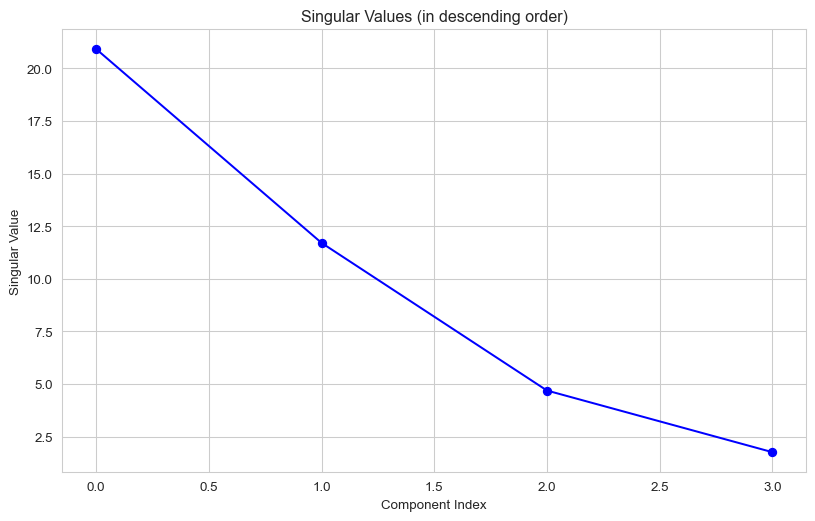
\includegraphics[keepaspectratio]{chapter5_files/figure-pdf/fig-svd-iris-output-2.png}}

}

\subcaption{\label{fig-svd-iris-1}SVD applied to the Iris dataset}

\centering{

\pandocbounded{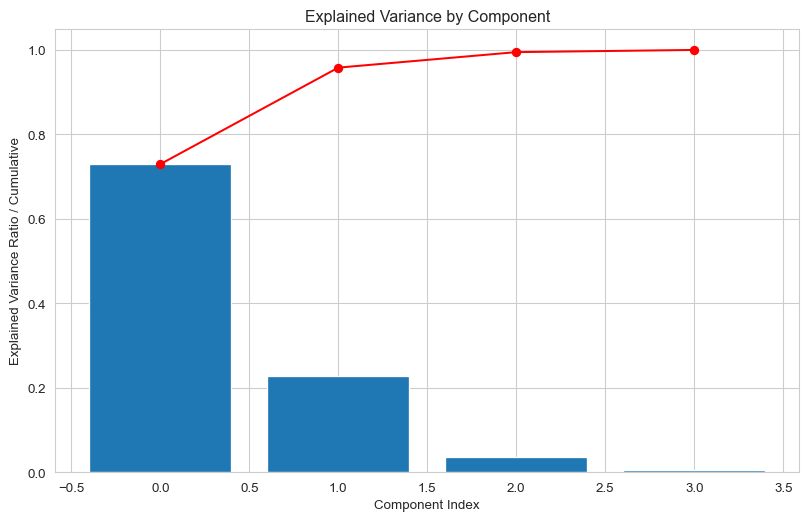
\includegraphics[keepaspectratio]{chapter5_files/figure-pdf/fig-svd-iris-output-3.png}}

}

\subcaption{\label{fig-svd-iris-2}}

}

\caption{\label{fig-svd-iris}}

\end{figure}%

\subsection{Relationship Between SVD and
PCA}\label{relationship-between-svd-and-pca}

PCA can be implemented using SVD, which is often more numerically
stable. The principal components in PCA are equivalent to the right
singular vectors in SVD.

\begin{Shaded}
\begin{Highlighting}[]
\CommentTok{\# Project data onto first two singular vectors (equivalent to first two PCs)}
\NormalTok{svd\_projection }\OperatorTok{=}\NormalTok{ X\_scaled }\OperatorTok{@}\NormalTok{ Vt.T[:, :}\DecValTok{2}\NormalTok{]}

\CommentTok{\# Visualize the projection}
\NormalTok{plt.figure(figsize}\OperatorTok{=}\NormalTok{(}\DecValTok{10}\NormalTok{, }\DecValTok{8}\NormalTok{))}
\NormalTok{colors }\OperatorTok{=}\NormalTok{ [}\StringTok{\textquotesingle{}navy\textquotesingle{}}\NormalTok{, }\StringTok{\textquotesingle{}turquoise\textquotesingle{}}\NormalTok{, }\StringTok{\textquotesingle{}darkorange\textquotesingle{}}\NormalTok{]}
\NormalTok{target\_names }\OperatorTok{=}\NormalTok{ iris.target\_names}

\ControlFlowTok{for}\NormalTok{ i, c, label }\KeywordTok{in} \BuiltInTok{zip}\NormalTok{(}\BuiltInTok{range}\NormalTok{(}\DecValTok{3}\NormalTok{), colors, target\_names):}
\NormalTok{    plt.scatter(svd\_projection[y }\OperatorTok{==}\NormalTok{ i, }\DecValTok{0}\NormalTok{], svd\_projection[y }\OperatorTok{==}\NormalTok{ i, }\DecValTok{1}\NormalTok{], }
\NormalTok{                c}\OperatorTok{=}\NormalTok{c, label}\OperatorTok{=}\NormalTok{label)}
    
\NormalTok{plt.xlabel(}\StringTok{\textquotesingle{}First Component\textquotesingle{}}\NormalTok{)}
\NormalTok{plt.ylabel(}\StringTok{\textquotesingle{}Second Component\textquotesingle{}}\NormalTok{)}
\NormalTok{plt.title(}\StringTok{\textquotesingle{}SVD Projection of Iris Dataset\textquotesingle{}}\NormalTok{)}
\NormalTok{plt.legend()}
\NormalTok{plt.grid(}\VariableTok{True}\NormalTok{)}
\NormalTok{plt.show()}

\CommentTok{\# Compare first two singular values with corresponding eigenvectors}
\BuiltInTok{print}\NormalTok{(}\SpecialStringTok{f"First two singular values: }\SpecialCharTok{\{}\NormalTok{sigma[:}\DecValTok{2}\NormalTok{]}\SpecialCharTok{\}}\SpecialStringTok{"}\NormalTok{)}
\BuiltInTok{print}\NormalTok{(}\SpecialStringTok{f"First two singular values squared: }\SpecialCharTok{\{}\NormalTok{sigma[:}\DecValTok{2}\NormalTok{]}\OperatorTok{**}\DecValTok{2}\SpecialCharTok{\}}\SpecialStringTok{"}\NormalTok{)}
\end{Highlighting}
\end{Shaded}

\begin{figure}[H]

\centering{

\pandocbounded{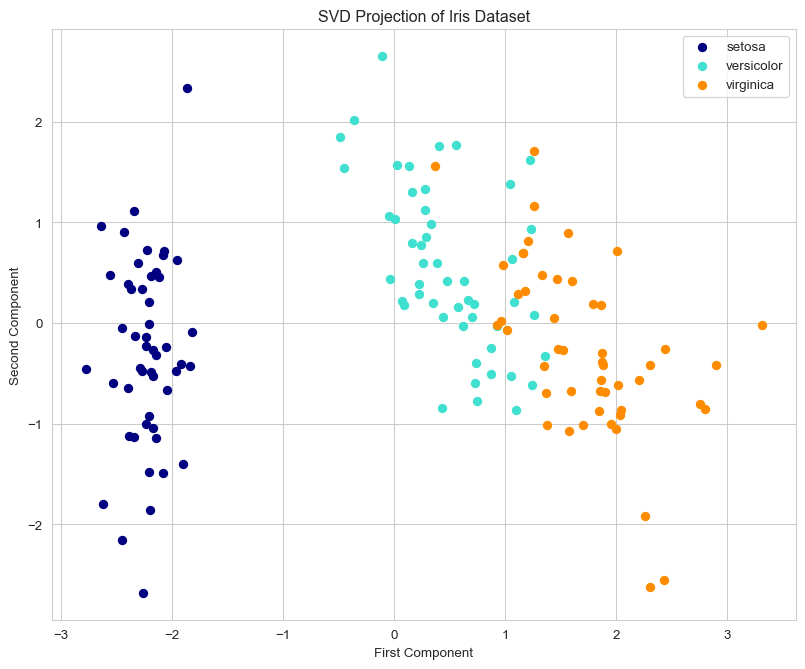
\includegraphics[keepaspectratio]{chapter5_files/figure-pdf/fig-svd-pca-comparison-output-1.png}}

}

\caption{\label{fig-svd-pca-comparison}Comparison of SVD and PCA
projections}

\end{figure}%

\begin{verbatim}
First two singular values: [20.92306556 11.7091661 ]
First two singular values squared: [437.77467248 137.10457072]
\end{verbatim}

\subsection{Low-Rank Approximation}\label{low-rank-approximation}

One of the key applications of SVD is low-rank matrix approximation,
which enables data compression:

\begin{Shaded}
\begin{Highlighting}[]
\CommentTok{\# Create a simple matrix for demonstration}
\NormalTok{A }\OperatorTok{=}\NormalTok{ np.array([}
\NormalTok{    [}\DecValTok{1}\NormalTok{, }\DecValTok{2}\NormalTok{, }\DecValTok{3}\NormalTok{, }\DecValTok{4}\NormalTok{, }\DecValTok{5}\NormalTok{],}
\NormalTok{    [}\DecValTok{6}\NormalTok{, }\DecValTok{7}\NormalTok{, }\DecValTok{8}\NormalTok{, }\DecValTok{9}\NormalTok{, }\DecValTok{10}\NormalTok{],}
\NormalTok{    [}\DecValTok{11}\NormalTok{, }\DecValTok{12}\NormalTok{, }\DecValTok{13}\NormalTok{, }\DecValTok{14}\NormalTok{, }\DecValTok{15}\NormalTok{]}
\NormalTok{])}

\CommentTok{\# Apply SVD}
\NormalTok{U, sigma, Vt }\OperatorTok{=}\NormalTok{ svd(A)}

\CommentTok{\# Create diagonal matrix Sigma}
\NormalTok{Sigma }\OperatorTok{=}\NormalTok{ np.zeros((A.shape[}\DecValTok{0}\NormalTok{], A.shape[}\DecValTok{1}\NormalTok{]))}
\ControlFlowTok{for}\NormalTok{ i }\KeywordTok{in} \BuiltInTok{range}\NormalTok{(}\BuiltInTok{min}\NormalTok{(A.shape)):}
\NormalTok{    Sigma[i, i] }\OperatorTok{=}\NormalTok{ sigma[i]}

\CommentTok{\# Function to reconstruct with k components}
\KeywordTok{def}\NormalTok{ reconstruct\_svd(u, sigma, vt, k):}
    \CommentTok{\# Create truncated sigma matrix}
\NormalTok{    sigma\_k }\OperatorTok{=}\NormalTok{ np.zeros((u.shape[}\DecValTok{0}\NormalTok{], vt.shape[}\DecValTok{0}\NormalTok{]))}
    \ControlFlowTok{for}\NormalTok{ i }\KeywordTok{in} \BuiltInTok{range}\NormalTok{(}\BuiltInTok{min}\NormalTok{(k, }\BuiltInTok{len}\NormalTok{(sigma))):}
\NormalTok{        sigma\_k[i, i] }\OperatorTok{=}\NormalTok{ sigma[i]}
    
    \CommentTok{\# Reconstruct}
    \ControlFlowTok{return}\NormalTok{ u }\OperatorTok{@}\NormalTok{ sigma\_k }\OperatorTok{@}\NormalTok{ vt}

\CommentTok{\# Reconstruct with different ranks}
\NormalTok{ranks }\OperatorTok{=}\NormalTok{ [}\DecValTok{1}\NormalTok{, }\DecValTok{2}\NormalTok{, }\DecValTok{3}\NormalTok{]}
\NormalTok{fig, axes }\OperatorTok{=}\NormalTok{ plt.subplots(}\DecValTok{1}\NormalTok{, }\BuiltInTok{len}\NormalTok{(ranks) }\OperatorTok{+} \DecValTok{1}\NormalTok{, figsize}\OperatorTok{=}\NormalTok{(}\DecValTok{15}\NormalTok{, }\DecValTok{4}\NormalTok{))}

\CommentTok{\# Original matrix}
\NormalTok{axes[}\DecValTok{0}\NormalTok{].imshow(A, cmap}\OperatorTok{=}\StringTok{\textquotesingle{}viridis\textquotesingle{}}\NormalTok{)}
\NormalTok{axes[}\DecValTok{0}\NormalTok{].set\_title(}\StringTok{\textquotesingle{}Original Matrix\textquotesingle{}}\NormalTok{)}
\NormalTok{axes[}\DecValTok{0}\NormalTok{].axis(}\StringTok{\textquotesingle{}off\textquotesingle{}}\NormalTok{)}

\CommentTok{\# Reconstructions}
\ControlFlowTok{for}\NormalTok{ i, k }\KeywordTok{in} \BuiltInTok{enumerate}\NormalTok{(ranks):}
\NormalTok{    A\_k }\OperatorTok{=}\NormalTok{ reconstruct\_svd(U, sigma, Vt, k)}
\NormalTok{    axes[i}\OperatorTok{+}\DecValTok{1}\NormalTok{].imshow(A\_k, cmap}\OperatorTok{=}\StringTok{\textquotesingle{}viridis\textquotesingle{}}\NormalTok{)}
\NormalTok{    axes[i}\OperatorTok{+}\DecValTok{1}\NormalTok{].set\_title(}\SpecialStringTok{f\textquotesingle{}Rank }\SpecialCharTok{\{}\NormalTok{k}\SpecialCharTok{\}}\SpecialStringTok{ Approximation\textquotesingle{}}\NormalTok{)}
\NormalTok{    axes[i}\OperatorTok{+}\DecValTok{1}\NormalTok{].axis(}\StringTok{\textquotesingle{}off\textquotesingle{}}\NormalTok{)}

\NormalTok{plt.tight\_layout()}
\NormalTok{plt.show()}

\CommentTok{\# Calculate and display approximation errors}
\ControlFlowTok{for}\NormalTok{ k }\KeywordTok{in}\NormalTok{ ranks:}
\NormalTok{    A\_k }\OperatorTok{=}\NormalTok{ reconstruct\_svd(U, sigma, Vt, k)}
\NormalTok{    error }\OperatorTok{=}\NormalTok{ np.linalg.norm(A }\OperatorTok{{-}}\NormalTok{ A\_k, }\StringTok{\textquotesingle{}fro\textquotesingle{}}\NormalTok{)}
    \BuiltInTok{print}\NormalTok{(}\SpecialStringTok{f"Rank }\SpecialCharTok{\{}\NormalTok{k}\SpecialCharTok{\}}\SpecialStringTok{ approximation error: }\SpecialCharTok{\{}\NormalTok{error}\SpecialCharTok{:.4f\}}\SpecialStringTok{"}\NormalTok{)}
\end{Highlighting}
\end{Shaded}

\begin{figure}[H]

\centering{

\pandocbounded{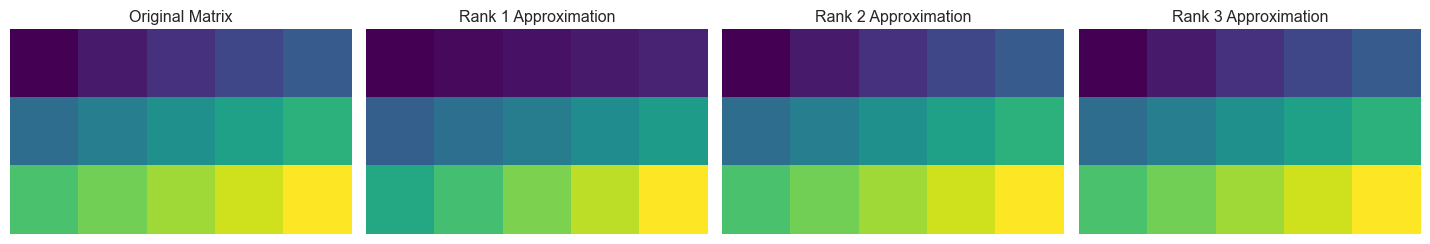
\includegraphics[keepaspectratio]{chapter5_files/figure-pdf/fig-svd-low-rank-output-1.png}}

}

\caption{\label{fig-svd-low-rank}Low-rank approximation of a matrix}

\end{figure}%

\begin{verbatim}
Rank 1 approximation error: 2.4654
Rank 2 approximation error: 0.0000
Rank 3 approximation error: 0.0000
\end{verbatim}

\subsection{SVD for Image Compression}\label{svd-for-image-compression}

A common application of SVD is image compression. Let's demonstrate this
with a grayscale image:

\begin{figure}

\centering{

\begin{Shaded}
\begin{Highlighting}[]
\CommentTok{\# Load a sample image}
\CommentTok{\# For demonstration, let\textquotesingle{}s create a simple gradient image}
\NormalTok{img\_size }\OperatorTok{=} \DecValTok{512}
\NormalTok{img }\OperatorTok{=}\NormalTok{ np.zeros((img\_size, img\_size))}
\ControlFlowTok{for}\NormalTok{ i }\KeywordTok{in} \BuiltInTok{range}\NormalTok{(img\_size):}
    \ControlFlowTok{for}\NormalTok{ j }\KeywordTok{in} \BuiltInTok{range}\NormalTok{(img\_size):}
\NormalTok{        img[i, j] }\OperatorTok{=}\NormalTok{ (i }\OperatorTok{+}\NormalTok{ j) }\OperatorTok{/}\NormalTok{ (}\DecValTok{2} \OperatorTok{*}\NormalTok{ img\_size)}

\CommentTok{\# Apply SVD}
\NormalTok{U, sigma, Vt }\OperatorTok{=}\NormalTok{ svd(img, full\_matrices}\OperatorTok{=}\VariableTok{False}\NormalTok{)}

\CommentTok{\# Compress image with different numbers of singular values}
\NormalTok{k\_values }\OperatorTok{=}\NormalTok{ [}\DecValTok{5}\NormalTok{, }\DecValTok{20}\NormalTok{, }\DecValTok{50}\NormalTok{, }\DecValTok{100}\NormalTok{]}
\NormalTok{fig, axes }\OperatorTok{=}\NormalTok{ plt.subplots(}\DecValTok{1}\NormalTok{, }\BuiltInTok{len}\NormalTok{(k\_values) }\OperatorTok{+} \DecValTok{1}\NormalTok{, figsize}\OperatorTok{=}\NormalTok{(}\DecValTok{18}\NormalTok{, }\DecValTok{4}\NormalTok{))}

\CommentTok{\# Original image}
\NormalTok{axes[}\DecValTok{0}\NormalTok{].imshow(img, cmap}\OperatorTok{=}\StringTok{\textquotesingle{}gray\textquotesingle{}}\NormalTok{)}
\NormalTok{axes[}\DecValTok{0}\NormalTok{].set\_title(}\StringTok{\textquotesingle{}Original Image\textquotesingle{}}\NormalTok{)}
\NormalTok{axes[}\DecValTok{0}\NormalTok{].axis(}\StringTok{\textquotesingle{}off\textquotesingle{}}\NormalTok{)}

\CommentTok{\# Compressed images}
\ControlFlowTok{for}\NormalTok{ i, k }\KeywordTok{in} \BuiltInTok{enumerate}\NormalTok{(k\_values):}
    \CommentTok{\# Reconstruct image with k singular values}
\NormalTok{    compressed\_img }\OperatorTok{=}\NormalTok{ U[:, :k] }\OperatorTok{@}\NormalTok{ np.diag(sigma[:k]) }\OperatorTok{@}\NormalTok{ Vt[:k, :]}
    
    \CommentTok{\# Display}
\NormalTok{    axes[i}\OperatorTok{+}\DecValTok{1}\NormalTok{].imshow(compressed\_img, cmap}\OperatorTok{=}\StringTok{\textquotesingle{}gray\textquotesingle{}}\NormalTok{)}
\NormalTok{    axes[i}\OperatorTok{+}\DecValTok{1}\NormalTok{].set\_title(}\SpecialStringTok{f\textquotesingle{}k=}\SpecialCharTok{\{}\NormalTok{k}\SpecialCharTok{\}}\SpecialStringTok{, CR=}\SpecialCharTok{\{}\NormalTok{img}\SpecialCharTok{.}\NormalTok{size}\OperatorTok{/}\NormalTok{(k}\OperatorTok{*}\NormalTok{(img.shape[}\DecValTok{0}\NormalTok{] }\OperatorTok{+}\NormalTok{ img.shape[}\DecValTok{1}\NormalTok{] }\OperatorTok{+} \DecValTok{1}\NormalTok{))}\SpecialCharTok{:.1f\}}\SpecialStringTok{\textquotesingle{}}\NormalTok{)}
\NormalTok{    axes[i}\OperatorTok{+}\DecValTok{1}\NormalTok{].axis(}\StringTok{\textquotesingle{}off\textquotesingle{}}\NormalTok{)}
    
    \CommentTok{\# Print compression ratio}
\NormalTok{    original\_size }\OperatorTok{=}\NormalTok{ img.size }\OperatorTok{*} \DecValTok{8}  \CommentTok{\# Assuming 8 bits per pixel}
\NormalTok{    compressed\_size }\OperatorTok{=}\NormalTok{ k }\OperatorTok{*}\NormalTok{ (img.shape[}\DecValTok{0}\NormalTok{] }\OperatorTok{+}\NormalTok{ img.shape[}\DecValTok{1}\NormalTok{] }\OperatorTok{+} \DecValTok{1}\NormalTok{) }\OperatorTok{*} \DecValTok{8}  \CommentTok{\# k(m+n+1) values stored}
\NormalTok{    compression\_ratio }\OperatorTok{=}\NormalTok{ original\_size }\OperatorTok{/}\NormalTok{ compressed\_size}
    \BuiltInTok{print}\NormalTok{(}\SpecialStringTok{f"k=}\SpecialCharTok{\{}\NormalTok{k}\SpecialCharTok{\}}\SpecialStringTok{, Compression ratio: }\SpecialCharTok{\{}\NormalTok{compression\_ratio}\SpecialCharTok{:.2f\}}\SpecialStringTok{"}\NormalTok{)}

\NormalTok{plt.tight\_layout()}
\NormalTok{plt.show()}
\end{Highlighting}
\end{Shaded}

}

\caption{\label{fig-image-compression}}

\end{figure}%

\subsection{Applications of SVD}\label{applications-of-svd}

SVD has numerous applications across various domains:

\subsubsection{1. Recommendation Systems}\label{recommendation-systems}

\begin{figure}

\centering{

\begin{Shaded}
\begin{Highlighting}[]
\CommentTok{\# Create a user{-}item ratings matrix (movies example)}
\CommentTok{\# Rows: users, Columns: movies, Values: ratings}
\NormalTok{ratings }\OperatorTok{=}\NormalTok{ np.array([}
\NormalTok{    [}\DecValTok{5}\NormalTok{, }\DecValTok{4}\NormalTok{, }\DecValTok{0}\NormalTok{, }\DecValTok{0}\NormalTok{, }\DecValTok{1}\NormalTok{],}
\NormalTok{    [}\DecValTok{4}\NormalTok{, }\DecValTok{0}\NormalTok{, }\DecValTok{0}\NormalTok{, }\DecValTok{3}\NormalTok{, }\DecValTok{1}\NormalTok{],}
\NormalTok{    [}\DecValTok{1}\NormalTok{, }\DecValTok{1}\NormalTok{, }\DecValTok{0}\NormalTok{, }\DecValTok{5}\NormalTok{, }\DecValTok{0}\NormalTok{],}
\NormalTok{    [}\DecValTok{0}\NormalTok{, }\DecValTok{0}\NormalTok{, }\DecValTok{4}\NormalTok{, }\DecValTok{0}\NormalTok{, }\DecValTok{3}\NormalTok{],}
\NormalTok{    [}\DecValTok{2}\NormalTok{, }\DecValTok{0}\NormalTok{, }\DecValTok{5}\NormalTok{, }\DecValTok{0}\NormalTok{, }\DecValTok{0}\NormalTok{]}
\NormalTok{])}

\CommentTok{\# Apply SVD}
\NormalTok{U, sigma, Vt }\OperatorTok{=}\NormalTok{ svd(ratings)}

\CommentTok{\# Use a low{-}rank approximation (k=2)}
\NormalTok{k }\OperatorTok{=} \DecValTok{2}
\NormalTok{ratings\_approx }\OperatorTok{=}\NormalTok{ U[:, :k] }\OperatorTok{@}\NormalTok{ np.diag(sigma[:k]) }\OperatorTok{@}\NormalTok{ Vt[:k, :]}

\CommentTok{\# Fill in missing ratings}
\BuiltInTok{print}\NormalTok{(}\StringTok{"Original ratings matrix:"}\NormalTok{)}
\BuiltInTok{print}\NormalTok{(ratings)}
\BuiltInTok{print}\NormalTok{(}\StringTok{"}\CharTok{\textbackslash{}n}\StringTok{Reconstructed ratings matrix:"}\NormalTok{)}
\BuiltInTok{print}\NormalTok{(np.}\BuiltInTok{round}\NormalTok{(ratings\_approx, }\DecValTok{1}\NormalTok{))}

\CommentTok{\# Find recommendations for a user}
\NormalTok{user\_id }\OperatorTok{=} \DecValTok{0}
\NormalTok{missing\_ratings }\OperatorTok{=}\NormalTok{ np.where(ratings[user\_id] }\OperatorTok{==} \DecValTok{0}\NormalTok{)[}\DecValTok{0}\NormalTok{]}
\NormalTok{recommendations }\OperatorTok{=}\NormalTok{ [(item, ratings\_approx[user\_id, item]) }\ControlFlowTok{for}\NormalTok{ item }\KeywordTok{in}\NormalTok{ missing\_ratings]}
\NormalTok{recommendations.sort(key}\OperatorTok{=}\KeywordTok{lambda}\NormalTok{ x: x[}\DecValTok{1}\NormalTok{], reverse}\OperatorTok{=}\VariableTok{True}\NormalTok{)}

\BuiltInTok{print}\NormalTok{(}\SpecialStringTok{f"}\CharTok{\textbackslash{}n}\SpecialStringTok{Top recommendations for User }\SpecialCharTok{\{}\NormalTok{user\_id}\SpecialCharTok{\}}\SpecialStringTok{:"}\NormalTok{)}
\ControlFlowTok{for}\NormalTok{ item, score }\KeywordTok{in}\NormalTok{ recommendations:}
    \BuiltInTok{print}\NormalTok{(}\SpecialStringTok{f"Item }\SpecialCharTok{\{}\NormalTok{item}\SpecialCharTok{\}}\SpecialStringTok{: Predicted rating }\SpecialCharTok{\{}\NormalTok{score}\SpecialCharTok{:.1f\}}\SpecialStringTok{"}\NormalTok{)}
\end{Highlighting}
\end{Shaded}

}

\caption{\label{fig-recommendation}}

\end{figure}%

\subsubsection{2. Latent Semantic Analysis (LSA) for Text
Mining}\label{latent-semantic-analysis-lsa-for-text-mining}

\begin{figure}

\centering{

\begin{Shaded}
\begin{Highlighting}[]
\ImportTok{from}\NormalTok{ sklearn.feature\_extraction.text }\ImportTok{import}\NormalTok{ TfidfVectorizer}
\ImportTok{from}\NormalTok{ sklearn.decomposition }\ImportTok{import}\NormalTok{ TruncatedSVD}

\CommentTok{\# Sample documents}
\NormalTok{documents }\OperatorTok{=}\NormalTok{ [}
    \StringTok{"Machine learning is a field of artificial intelligence"}\NormalTok{,}
    \StringTok{"Deep learning is a subset of machine learning"}\NormalTok{,}
    \StringTok{"Neural networks are used in deep learning"}\NormalTok{,}
    \StringTok{"SVD is used for dimensionality reduction"}\NormalTok{,}
    \StringTok{"PCA and SVD are related techniques"}\NormalTok{,}
    \StringTok{"Dimensionality reduction helps with visualizing data"}
\NormalTok{]}

\CommentTok{\# Create TF{-}IDF matrix}
\NormalTok{vectorizer }\OperatorTok{=}\NormalTok{ TfidfVectorizer(stop\_words}\OperatorTok{=}\StringTok{\textquotesingle{}english\textquotesingle{}}\NormalTok{)}
\NormalTok{X }\OperatorTok{=}\NormalTok{ vectorizer.fit\_transform(documents)}

\CommentTok{\# Get feature names}
\NormalTok{feature\_names }\OperatorTok{=}\NormalTok{ vectorizer.get\_feature\_names\_out()}

\CommentTok{\# Print the document{-}term matrix}
\BuiltInTok{print}\NormalTok{(}\StringTok{"Document{-}Term Matrix (TF{-}IDF):"}\NormalTok{)}
\NormalTok{df }\OperatorTok{=}\NormalTok{ pd.DataFrame(X.toarray(), columns}\OperatorTok{=}\NormalTok{feature\_names)}
\BuiltInTok{print}\NormalTok{(df)}

\CommentTok{\# Apply LSA (truncated SVD)}
\NormalTok{n\_components }\OperatorTok{=} \DecValTok{2}
\NormalTok{lsa }\OperatorTok{=}\NormalTok{ TruncatedSVD(n\_components}\OperatorTok{=}\NormalTok{n\_components)}
\NormalTok{X\_lsa }\OperatorTok{=}\NormalTok{ lsa.fit\_transform(X)}

\CommentTok{\# Print explained variance}
\BuiltInTok{print}\NormalTok{(}\SpecialStringTok{f"}\CharTok{\textbackslash{}n}\SpecialStringTok{Explained variance ratio: }\SpecialCharTok{\{}\NormalTok{lsa}\SpecialCharTok{.}\NormalTok{explained\_variance\_ratio\_}\SpecialCharTok{\}}\SpecialStringTok{"}\NormalTok{)}
\BuiltInTok{print}\NormalTok{(}\SpecialStringTok{f"Total explained variance: }\SpecialCharTok{\{}\BuiltInTok{sum}\NormalTok{(lsa.explained\_variance\_ratio\_)}\SpecialCharTok{:.2f\}}\SpecialStringTok{"}\NormalTok{)}

\CommentTok{\# Plot documents in the reduced space}
\NormalTok{plt.figure(figsize}\OperatorTok{=}\NormalTok{(}\DecValTok{10}\NormalTok{, }\DecValTok{8}\NormalTok{))}
\NormalTok{plt.scatter(X\_lsa[:, }\DecValTok{0}\NormalTok{], X\_lsa[:, }\DecValTok{1}\NormalTok{], alpha}\OperatorTok{=}\FloatTok{0.8}\NormalTok{)}

\CommentTok{\# Label each point}
\ControlFlowTok{for}\NormalTok{ i, doc }\KeywordTok{in} \BuiltInTok{enumerate}\NormalTok{(documents):}
\NormalTok{    plt.annotate(}\SpecialStringTok{f"Doc }\SpecialCharTok{\{}\NormalTok{i}\OperatorTok{+}\DecValTok{1}\SpecialCharTok{\}}\SpecialStringTok{"}\NormalTok{, (X\_lsa[i, }\DecValTok{0}\NormalTok{], X\_lsa[i, }\DecValTok{1}\NormalTok{]), }
\NormalTok{                 xytext}\OperatorTok{=}\NormalTok{(}\DecValTok{5}\NormalTok{, }\DecValTok{5}\NormalTok{), textcoords}\OperatorTok{=}\StringTok{\textquotesingle{}offset points\textquotesingle{}}\NormalTok{)}

\NormalTok{plt.xlabel(}\StringTok{"Component 1"}\NormalTok{)}
\NormalTok{plt.ylabel(}\StringTok{"Component 2"}\NormalTok{)}
\NormalTok{plt.title(}\StringTok{"Documents in LSA Space"}\NormalTok{)}
\NormalTok{plt.grid(}\VariableTok{True}\NormalTok{)}
\NormalTok{plt.show()}

\CommentTok{\# Examine term weights in components}
\NormalTok{component\_terms }\OperatorTok{=}\NormalTok{ \{\}}
\ControlFlowTok{for}\NormalTok{ i, component }\KeywordTok{in} \BuiltInTok{enumerate}\NormalTok{(lsa.components\_):}
    \CommentTok{\# Get the top terms for this component}
\NormalTok{    terms }\OperatorTok{=} \BuiltInTok{zip}\NormalTok{(feature\_names, component)}
\NormalTok{    sorted\_terms }\OperatorTok{=} \BuiltInTok{sorted}\NormalTok{(terms, key}\OperatorTok{=}\KeywordTok{lambda}\NormalTok{ x: }\BuiltInTok{abs}\NormalTok{(x[}\DecValTok{1}\NormalTok{]), reverse}\OperatorTok{=}\VariableTok{True}\NormalTok{)[:}\DecValTok{5}\NormalTok{]}
\NormalTok{    component\_terms[}\SpecialStringTok{f"Component }\SpecialCharTok{\{}\NormalTok{i}\OperatorTok{+}\DecValTok{1}\SpecialCharTok{\}}\SpecialStringTok{"}\NormalTok{] }\OperatorTok{=}\NormalTok{ sorted\_terms}

\CommentTok{\# Display top terms for each component}
\ControlFlowTok{for}\NormalTok{ component, terms }\KeywordTok{in}\NormalTok{ component\_terms.items():}
    \BuiltInTok{print}\NormalTok{(}\SpecialStringTok{f"}\CharTok{\textbackslash{}n}\SpecialCharTok{\{}\NormalTok{component}\SpecialCharTok{\}}\SpecialStringTok{ top terms:"}\NormalTok{)}
    \ControlFlowTok{for}\NormalTok{ term, weight }\KeywordTok{in}\NormalTok{ terms:}
        \BuiltInTok{print}\NormalTok{(}\SpecialStringTok{f"  }\SpecialCharTok{\{}\NormalTok{term}\SpecialCharTok{\}}\SpecialStringTok{: }\SpecialCharTok{\{}\NormalTok{weight}\SpecialCharTok{:.3f\}}\SpecialStringTok{"}\NormalTok{)}
\end{Highlighting}
\end{Shaded}

}

\caption{\label{fig-lsa}}

\end{figure}%

\subsection{Truncated SVD vs.~PCA}\label{truncated-svd-vs.-pca}

Truncated SVD can be applied directly to sparse matrices, while PCA
typically requires dense matrices. This makes Truncated SVD particularly
useful for text analysis and high-dimensional sparse data:

\begin{Shaded}
\begin{Highlighting}[]
\ImportTok{from}\NormalTok{ sklearn.decomposition }\ImportTok{import}\NormalTok{ TruncatedSVD, PCA}
\ImportTok{from}\NormalTok{ scipy.sparse }\ImportTok{import}\NormalTok{ csr\_matrix}

\CommentTok{\# Create a sparse matrix}
\NormalTok{rows }\OperatorTok{=}\NormalTok{ np.random.randint(}\DecValTok{0}\NormalTok{, }\DecValTok{100}\NormalTok{, }\DecValTok{1000}\NormalTok{)}
\NormalTok{cols }\OperatorTok{=}\NormalTok{ np.random.randint(}\DecValTok{0}\NormalTok{, }\DecValTok{50}\NormalTok{, }\DecValTok{1000}\NormalTok{)}
\NormalTok{data }\OperatorTok{=}\NormalTok{ np.random.randn(}\DecValTok{1000}\NormalTok{)}
\NormalTok{sparse\_matrix }\OperatorTok{=}\NormalTok{ csr\_matrix((data, (rows, cols)), shape}\OperatorTok{=}\NormalTok{(}\DecValTok{100}\NormalTok{, }\DecValTok{50}\NormalTok{))}

\CommentTok{\# Apply Truncated SVD}
\NormalTok{tsvd }\OperatorTok{=}\NormalTok{ TruncatedSVD(n\_components}\OperatorTok{=}\DecValTok{2}\NormalTok{)}
\NormalTok{tsvd\_result }\OperatorTok{=}\NormalTok{ tsvd.fit\_transform(sparse\_matrix)}

\CommentTok{\# Convert to dense for PCA}
\NormalTok{dense\_matrix }\OperatorTok{=}\NormalTok{ sparse\_matrix.toarray()}

\CommentTok{\# Apply PCA}
\NormalTok{pca }\OperatorTok{=}\NormalTok{ PCA(n\_components}\OperatorTok{=}\DecValTok{2}\NormalTok{)}
\NormalTok{pca\_result }\OperatorTok{=}\NormalTok{ pca.fit\_transform(dense\_matrix)}

\CommentTok{\# Compare results}
\NormalTok{fig, axes }\OperatorTok{=}\NormalTok{ plt.subplots(}\DecValTok{1}\NormalTok{, }\DecValTok{2}\NormalTok{, figsize}\OperatorTok{=}\NormalTok{(}\DecValTok{14}\NormalTok{, }\DecValTok{6}\NormalTok{))}

\CommentTok{\# Plot Truncated SVD result}
\NormalTok{axes[}\DecValTok{0}\NormalTok{].scatter(tsvd\_result[:, }\DecValTok{0}\NormalTok{], tsvd\_result[:, }\DecValTok{1}\NormalTok{], alpha}\OperatorTok{=}\FloatTok{0.5}\NormalTok{)}
\NormalTok{axes[}\DecValTok{0}\NormalTok{].set\_title(}\StringTok{\textquotesingle{}Truncated SVD\textquotesingle{}}\NormalTok{)}
\NormalTok{axes[}\DecValTok{0}\NormalTok{].set\_xlabel(}\StringTok{\textquotesingle{}Component 1\textquotesingle{}}\NormalTok{)}
\NormalTok{axes[}\DecValTok{0}\NormalTok{].set\_ylabel(}\StringTok{\textquotesingle{}Component 2\textquotesingle{}}\NormalTok{)}
\NormalTok{axes[}\DecValTok{0}\NormalTok{].grid(}\VariableTok{True}\NormalTok{)}

\CommentTok{\# Plot PCA result}
\NormalTok{axes[}\DecValTok{1}\NormalTok{].scatter(pca\_result[:, }\DecValTok{0}\NormalTok{], pca\_result[:, }\DecValTok{1}\NormalTok{], alpha}\OperatorTok{=}\FloatTok{0.5}\NormalTok{)}
\NormalTok{axes[}\DecValTok{1}\NormalTok{].set\_title(}\StringTok{\textquotesingle{}PCA\textquotesingle{}}\NormalTok{)}
\NormalTok{axes[}\DecValTok{1}\NormalTok{].set\_xlabel(}\StringTok{\textquotesingle{}Component 1\textquotesingle{}}\NormalTok{)}
\NormalTok{axes[}\DecValTok{1}\NormalTok{].set\_ylabel(}\StringTok{\textquotesingle{}Component 2\textquotesingle{}}\NormalTok{)}
\NormalTok{axes[}\DecValTok{1}\NormalTok{].grid(}\VariableTok{True}\NormalTok{)}

\NormalTok{plt.tight\_layout()}
\NormalTok{plt.show()}

\CommentTok{\# Compare explained variance}
\BuiltInTok{print}\NormalTok{(}\SpecialStringTok{f"Truncated SVD explained variance ratio: }\SpecialCharTok{\{}\NormalTok{tsvd}\SpecialCharTok{.}\NormalTok{explained\_variance\_ratio\_}\SpecialCharTok{\}}\SpecialStringTok{"}\NormalTok{)}
\BuiltInTok{print}\NormalTok{(}\SpecialStringTok{f"PCA explained variance ratio: }\SpecialCharTok{\{}\NormalTok{pca}\SpecialCharTok{.}\NormalTok{explained\_variance\_ratio\_}\SpecialCharTok{\}}\SpecialStringTok{"}\NormalTok{)}
\end{Highlighting}
\end{Shaded}

\begin{figure}[H]

\centering{

\pandocbounded{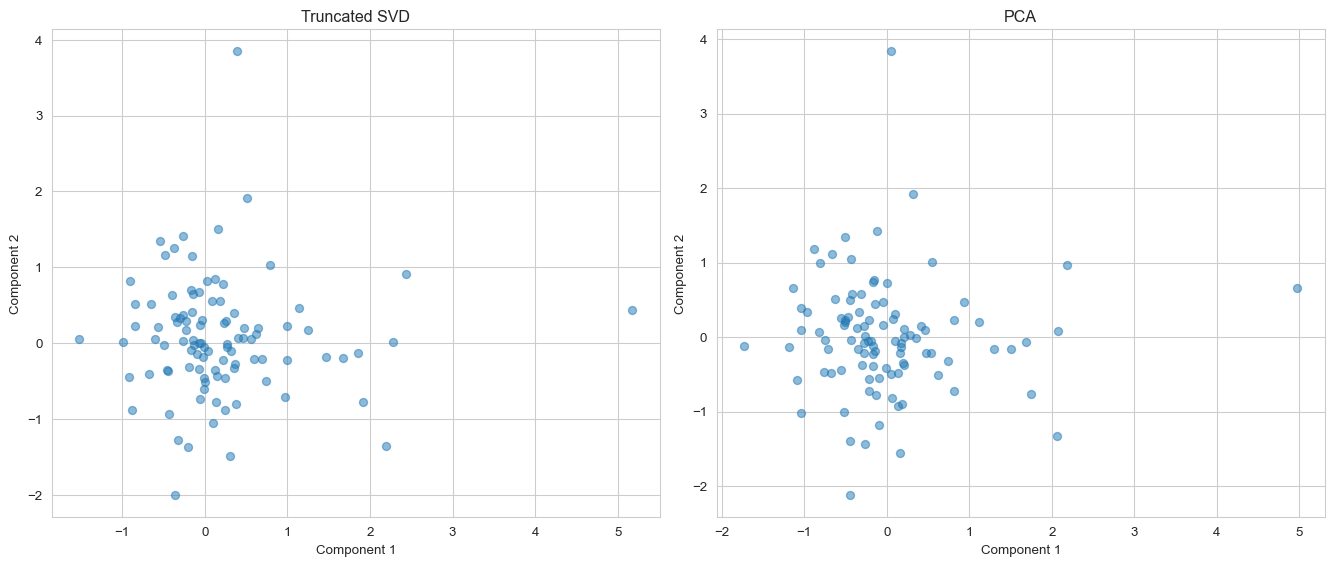
\includegraphics[keepaspectratio]{chapter5_files/figure-pdf/fig-truncated-svd-output-1.png}}

}

\caption{\label{fig-truncated-svd}Comparison of Truncated SVD and PCA}

\end{figure}%

\begin{verbatim}
Truncated SVD explained variance ratio: [0.06312201 0.05684404]
PCA explained variance ratio: [0.06325335 0.05699384]
\end{verbatim}

\section{No\# Advantages and Limitations of
SVD}\label{no-advantages-and-limitations-of-svd}

\subsubsection{Advantages}\label{advantages-1}

\begin{enumerate}
\def\labelenumi{\arabic{enumi}.}
\tightlist
\item
  \textbf{Robust mathematical foundation}: Based on well-established
  linear algebra principles
\item
  \textbf{Numerical stability}: Often more stable than
  eigendecomposition-based methods
\item
  \textbf{Applicability to non-square matrices}: Can be applied to any
  rectangular matrix
\item
  \textbf{Optimal low-rank approximation}: Provides the best
  approximation in terms of Frobenius norm
\end{enumerate}

\subsubsection{Limitations}\label{limitations}

\begin{enumerate}
\def\labelenumi{\arabic{enumi}.}
\tightlist
\item
  \textbf{Computational cost}: Full SVD is expensive for large matrices
  (O(min(mn², m²n)))
\item
  \textbf{Memory requirements}: Working with large matrices can be
  memory-intensive
\item
  \textbf{Interpretability}: The resulting components may be difficult
  to interpret in some domains
\item
  \textbf{Linearity}: As with PCA, SVD assumes linear relationships in
  the data
\end{enumerate}

\section{Conclusion}\label{conclusion}

Dimensionality reduction techniques are essential tools in the data
scientist's toolkit, enabling:

\begin{itemize}
\tightlist
\item
  More efficient model training
\item
  Better visualization of complex datasets
\item
  Improved performance through noise reduction
\item
  Insights into feature importance and relationships
\end{itemize}

As with all techniques, the choice of dimensionality reduction method
should be guided by:

\begin{enumerate}
\def\labelenumi{\arabic{enumi}.}
\tightlist
\item
  The specific characteristics of your dataset
\item
  Your analysis goals
\item
  Computational constraints
\item
  Whether you need interpretable results
\end{enumerate}

Singular Value Decomposition is a fundamental technique in linear
algebra with powerful applications in dimensionality reduction, data
compression, noise filtering, and recommendation systems. Its ability to
decompose any matrix into meaningful components makes it an essential
tool for data scientists and machine learning practitioners.

By understanding the mathematical principles behind SVD and its
relationship to other dimensionality reduction techniques like PCA, we
can effectively apply it to solve complex problems across various
domains.

In practice, the choice between full SVD, truncated SVD, or randomized
algorithms depends on the specific characteristics of the data and
computational constraints. Modern implementations in libraries like
SciPy and scikit-learn provide efficient algorithms that make SVD
accessible for large-scale applications.

The Python implementations demonstrated in this document provide a
starting point for applying these techniques to your own data analysis
and machine learning projects.

\section{References}\label{references}

\begin{enumerate}
\def\labelenumi{\arabic{enumi}.}
\tightlist
\item
  Jolliffe, I. T., \& Cadima, J. (2016). Principal component analysis: a
  review and recent developments. Philosophical Transactions of the
  Royal Society A, 374(2065).
\item
  Van der Maaten, L., \& Hinton, G. (2008). Visualizing data using
  t-SNE. Journal of Machine Learning Research, 9(11).
\item
  Pedregosa, F., et al.~(2011). Scikit-learn: Machine Learning in
  Python. Journal of Machine Learning Research, 12, 2825-2830.
\end{enumerate}

\bookmarksetup{startatroot}

\chapter{Tree-Based Models and Ensemble
Learning}\label{tree-based-models-and-ensemble-learning}

\section{Decision Trees}\label{decision-trees}

Decision trees are versatile machine learning models that can handle
both classification and regression tasks. They're powerful tools for
inductive inference and particularly useful for approximating
discrete-valued target functions.

\subsection{Key Features}\label{key-features}

\begin{itemize}
\tightlist
\item
  \textbf{Robust to Noisy Data}: Handle imperfections in data, including
  noise and missing values
\item
  \textbf{Complex Datasets}: Capable of fitting complex datasets and
  representing disjunctive expressions
\item
  \textbf{Interpretable}: Trees model decisions through a series of
  ``if/else'' questions, providing clear decision-making processes
\end{itemize}

\subsection{Core Concepts}\label{core-concepts}

Decision trees operate by recursively partitioning the feature space
based on the values of input features. At each node:

\begin{enumerate}
\def\labelenumi{\arabic{enumi}.}
\tightlist
\item
  \textbf{Feature Selection}: Choose the most informative feature to
  split on
\item
  \textbf{Splitting Criterion}: Determine the optimal threshold or
  condition for the split
\item
  \textbf{Recursive Partitioning}: Continue splitting until stopping
  criteria are met
\end{enumerate}

The algorithm aims to create homogeneous subsets with respect to the
target variable, maximizing information gain at each step.

\subsection{Decision Boundaries}\label{decision-boundaries}

Decision trees create piecewise constant decision boundaries that are
parallel to the feature axes. This characteristic leads to:

\begin{itemize}
\tightlist
\item
  \textbf{Rectangular Partitioning}: Each leaf represents a rectangular
  region in the feature space
\item
  \textbf{Orthogonal Boundaries}: Decision boundaries are always
  perpendicular to feature axes
\item
  \textbf{Staircase Effect}: Complex functions are approximated using
  axis-parallel rectangles
\end{itemize}

\begin{Shaded}
\begin{Highlighting}[]
\ImportTok{import}\NormalTok{ numpy }\ImportTok{as}\NormalTok{ np}
\ImportTok{import}\NormalTok{ matplotlib.pyplot }\ImportTok{as}\NormalTok{ plt}
\ImportTok{from}\NormalTok{ sklearn.datasets }\ImportTok{import}\NormalTok{ load\_iris}
\ImportTok{from}\NormalTok{ sklearn.tree }\ImportTok{import}\NormalTok{ DecisionTreeClassifier, plot\_tree}
\ImportTok{from}\NormalTok{ sklearn.model\_selection }\ImportTok{import}\NormalTok{ train\_test\_split}

\CommentTok{\# Load dataset}
\NormalTok{iris }\OperatorTok{=}\NormalTok{ load\_iris()}
\NormalTok{X, y }\OperatorTok{=}\NormalTok{ iris.data, iris.target}

\CommentTok{\# Split data}
\NormalTok{X\_train, X\_test, y\_train, y\_test }\OperatorTok{=}\NormalTok{ train\_test\_split(X, y, test\_size}\OperatorTok{=}\FloatTok{0.3}\NormalTok{, random\_state}\OperatorTok{=}\DecValTok{42}\NormalTok{)}

\CommentTok{\# Create and train decision tree}
\NormalTok{clf }\OperatorTok{=}\NormalTok{ DecisionTreeClassifier(max\_depth}\OperatorTok{=}\DecValTok{3}\NormalTok{, random\_state}\OperatorTok{=}\DecValTok{42}\NormalTok{)}
\NormalTok{clf.fit(X\_train, y\_train)}

\CommentTok{\# Visualize decision tree}
\NormalTok{plt.figure(figsize}\OperatorTok{=}\NormalTok{(}\DecValTok{12}\NormalTok{, }\DecValTok{8}\NormalTok{))}
\NormalTok{plot\_tree(clf, filled}\OperatorTok{=}\VariableTok{True}\NormalTok{, feature\_names}\OperatorTok{=}\NormalTok{iris.feature\_names, class\_names}\OperatorTok{=}\NormalTok{iris.target\_names)}
\NormalTok{plt.title(}\StringTok{"Decision Tree on Iris Dataset"}\NormalTok{)}
\NormalTok{plt.show()}

\CommentTok{\# Evaluate performance}
\NormalTok{train\_score }\OperatorTok{=}\NormalTok{ clf.score(X\_train, y\_train)}
\NormalTok{test\_score }\OperatorTok{=}\NormalTok{ clf.score(X\_test, y\_test)}
\BuiltInTok{print}\NormalTok{(}\SpecialStringTok{f"Training accuracy: }\SpecialCharTok{\{}\NormalTok{train\_score}\SpecialCharTok{:.3f\}}\SpecialStringTok{"}\NormalTok{)}
\BuiltInTok{print}\NormalTok{(}\SpecialStringTok{f"Testing accuracy: }\SpecialCharTok{\{}\NormalTok{test\_score}\SpecialCharTok{:.3f\}}\SpecialStringTok{"}\NormalTok{)}
\end{Highlighting}
\end{Shaded}

\pandocbounded{\includegraphics[keepaspectratio]{chapter6_files/figure-pdf/cell-2-output-1.png}}

\begin{verbatim}
Training accuracy: 0.952
Testing accuracy: 1.000
\end{verbatim}

\subsection{Representation}\label{representation}

Decision trees represent a disjunction (OR) of conjunctions (AND) of
constraints on attribute values:

\begin{itemize}
\tightlist
\item
  Each path from root to leaf represents a conjunction (AND) of tests on
  instance attributes
\item
  The entire tree is a disjunction (OR) of these conjunctions
\item
  Each leaf node represents a classification outcome
\end{itemize}

\subsection{When to Use Decision
Trees}\label{when-to-use-decision-trees}

\begin{itemize}
\tightlist
\item
  \textbf{Attribute-Value Pair Representation}: Instances are
  represented as attribute-value pairs
\item
  \textbf{Discrete Output}: Target function has discrete output values
  (classification tasks)
\item
  \textbf{Disjunctive Descriptions}: Need to represent logical ORs
\item
  \textbf{Noisy Data}: Training data contains errors or missing values
\end{itemize}

\subsection{Classification Process}\label{classification-process}

Trees classify instances by sorting them from root to leaf: - Each node
tests an attribute - Each branch corresponds to a possible attribute
value - Each leaf assigns a class label

\subsection{Algorithmic Approaches}\label{algorithmic-approaches}

Several algorithms exist for constructing decision trees:

\begin{enumerate}
\def\labelenumi{\arabic{enumi}.}
\tightlist
\item
  \textbf{ID3 (Iterative Dichotomiser 3)}: Uses entropy and information
  gain
\item
  \textbf{C4.5}: Extends ID3 by handling continuous attributes and
  missing values
\item
  \textbf{CART (Classification and Regression Trees)}: Uses Gini
  impurity for classification
\item
  \textbf{CHAID (Chi-square Automatic Interaction Detector)}: Uses
  chi-square tests for categorical outputs
\end{enumerate}

\subsection{The CART Algorithm}\label{the-cart-algorithm}

CART (Classification and Regression Trees) is one of the most popular
decision tree algorithms:

\begin{enumerate}
\def\labelenumi{\arabic{enumi}.}
\tightlist
\item
  Start with all data at the root node
\item
  For each feature, find the best split that minimizes impurity
\item
  Split the data based on the best feature and threshold
\item
  Recursively apply steps 2-3 to the child nodes
\item
  Stop when a stopping criterion is met (e.g., max depth, min samples)
\end{enumerate}

\subsection{Training a Decision Tree}\label{training-a-decision-tree}

The training process involves finding the best set of questions (splits)
to divide the data:

\begin{Shaded}
\begin{Highlighting}[]
\KeywordTok{class}\NormalTok{ Leaf:}
    \KeywordTok{def} \FunctionTok{\_\_init\_\_}\NormalTok{(}\VariableTok{self}\NormalTok{, value):}
        \VariableTok{self}\NormalTok{.value }\OperatorTok{=}\NormalTok{ value}

\KeywordTok{class}\NormalTok{ Node:}
    \KeywordTok{def} \FunctionTok{\_\_init\_\_}\NormalTok{(}\VariableTok{self}\NormalTok{, attribute):}
        \VariableTok{self}\NormalTok{.attribute }\OperatorTok{=}\NormalTok{ attribute}
        \VariableTok{self}\NormalTok{.branches }\OperatorTok{=}\NormalTok{ \{\}}

    \KeywordTok{def}\NormalTok{ add\_branch(}\VariableTok{self}\NormalTok{, value, subtree):}
        \VariableTok{self}\NormalTok{.branches[value] }\OperatorTok{=}\NormalTok{ subtree}

\KeywordTok{def}\NormalTok{ basic\_decision\_tree\_algorithm(examples, target\_attribute, attributes):}
    \CommentTok{"""}
\CommentTok{    Basic implementation of a decision tree algorithm}
\CommentTok{    """}
    \CommentTok{\# If all examples have the same value for the target attribute, return a leaf node}
    \ControlFlowTok{if} \BuiltInTok{len}\NormalTok{(}\BuiltInTok{set}\NormalTok{(ex[target\_attribute] }\ControlFlowTok{for}\NormalTok{ ex }\KeywordTok{in}\NormalTok{ examples)) }\OperatorTok{==} \DecValTok{1}\NormalTok{:}
        \ControlFlowTok{return}\NormalTok{ Leaf(examples[}\DecValTok{0}\NormalTok{][target\_attribute])}
    
    \CommentTok{\# If no attributes are left, return a leaf node with the majority value}
    \ControlFlowTok{if} \KeywordTok{not}\NormalTok{ attributes:}
\NormalTok{        majority\_value }\OperatorTok{=} \BuiltInTok{max}\NormalTok{(}\BuiltInTok{set}\NormalTok{(ex[target\_attribute] }\ControlFlowTok{for}\NormalTok{ ex }\KeywordTok{in}\NormalTok{ examples), key}\OperatorTok{=}\KeywordTok{lambda}\NormalTok{ val: }\BuiltInTok{sum}\NormalTok{(ex[target\_attribute] }\OperatorTok{==}\NormalTok{ val }\ControlFlowTok{for}\NormalTok{ ex }\KeywordTok{in}\NormalTok{ examples))}
        \ControlFlowTok{return}\NormalTok{ Leaf(majority\_value)}
    
    \CommentTok{\# Choose the best attribute to split on (placeholder for actual selection logic)}
\NormalTok{    best\_attribute }\OperatorTok{=}\NormalTok{ attributes[}\DecValTok{0}\NormalTok{]  }\CommentTok{\# Replace with actual logic to select the best attribute}
    
    \CommentTok{\# Create a new decision tree node}
\NormalTok{    tree }\OperatorTok{=}\NormalTok{ Node(best\_attribute)}
    
    \CommentTok{\# Get unique values for the best attribute}
\NormalTok{    unique\_values }\OperatorTok{=} \BuiltInTok{set}\NormalTok{(ex[best\_attribute] }\ControlFlowTok{for}\NormalTok{ ex }\KeywordTok{in}\NormalTok{ examples)}
    
    \ControlFlowTok{for}\NormalTok{ value }\KeywordTok{in}\NormalTok{ unique\_values:}
        \CommentTok{\# Create a subset of examples where the best attribute equals the current value}
\NormalTok{        subset }\OperatorTok{=}\NormalTok{ [ex }\ControlFlowTok{for}\NormalTok{ ex }\KeywordTok{in}\NormalTok{ examples }\ControlFlowTok{if}\NormalTok{ ex[best\_attribute] }\OperatorTok{==}\NormalTok{ value]}
        
        \ControlFlowTok{if} \KeywordTok{not}\NormalTok{ subset:}
            \CommentTok{\# If the subset is empty, add a leaf with the majority value}
\NormalTok{            majority\_value }\OperatorTok{=} \BuiltInTok{max}\NormalTok{(}\BuiltInTok{set}\NormalTok{(ex[target\_attribute] }\ControlFlowTok{for}\NormalTok{ ex }\KeywordTok{in}\NormalTok{ examples), key}\OperatorTok{=}\KeywordTok{lambda}\NormalTok{ val: }\BuiltInTok{sum}\NormalTok{(ex[target\_attribute] }\OperatorTok{==}\NormalTok{ val }\ControlFlowTok{for}\NormalTok{ ex }\KeywordTok{in}\NormalTok{ examples))}
\NormalTok{            tree.add\_branch(value, Leaf(majority\_value))}
        \ControlFlowTok{else}\NormalTok{:}
            \CommentTok{\# Recursively build the subtree}
\NormalTok{            subtree }\OperatorTok{=}\NormalTok{ basic\_decision\_tree\_algorithm(subset, target\_attribute, [attr }\ControlFlowTok{for}\NormalTok{ attr }\KeywordTok{in}\NormalTok{ attributes }\ControlFlowTok{if}\NormalTok{ attr }\OperatorTok{!=}\NormalTok{ best\_attribute])}
\NormalTok{            tree.add\_branch(value, subtree)}
    
    \ControlFlowTok{return}\NormalTok{ tree}
\end{Highlighting}
\end{Shaded}

\subsubsection{Impurity Measures}\label{impurity-measures}

To decide the best feature to split on, decision trees use impurity
measures:

\begin{itemize}
\tightlist
\item
  \textbf{Gini Index}: Measures the likelihood of misclassifying a
  randomly selected instance
\item
  \textbf{Entropy}: Measures disorder or uncertainty in the dataset
\item
  \textbf{Misclassification Error}: Proportion of misclassified
  instances
\end{itemize}

\paragraph{Entropy}\label{entropy}

Entropy quantifies the uncertainty or randomness in a set of examples:

\(H(S) = -\sum_{i=1}^{c} p_i \log_2(p_i)\)

Where: - \(S\) is the dataset - \(c\) is the number of classes - \(p_i\)
is the proportion of examples in class \(i\)

\paragraph{Information Gain}\label{information-gain}

Information gain measures the reduction in entropy after splitting on an
attribute:

\(IG(S, A) = H(S) - \sum_{v \in Values(A)} \frac{|S_v|}{|S|} H(S_v)\)

Where: - \(A\) is the attribute - \(S_v\) is the subset of \(S\) for
which attribute \(A\) has value \(v\)

\paragraph{Gini Impurity}\label{gini-impurity}

Gini impurity measures the probability of incorrectly classifying a
randomly chosen element if it were randomly labeled according to the
class distribution in the subset:

\(Gini(S) = 1 - \sum_{i=1}^{c} (p_i)^2\)

\begin{Shaded}
\begin{Highlighting}[]
\KeywordTok{def}\NormalTok{ calculate\_entropy(y):}
    \CommentTok{"""Calculate entropy of a label set"""}
\NormalTok{    classes, counts }\OperatorTok{=}\NormalTok{ np.unique(y, return\_counts}\OperatorTok{=}\VariableTok{True}\NormalTok{)}
\NormalTok{    probabilities }\OperatorTok{=}\NormalTok{ counts }\OperatorTok{/}\NormalTok{ counts.}\BuiltInTok{sum}\NormalTok{()}
\NormalTok{    entropy }\OperatorTok{=} \OperatorTok{{-}}\NormalTok{np.}\BuiltInTok{sum}\NormalTok{(probabilities }\OperatorTok{*}\NormalTok{ np.log2(probabilities))}
    \ControlFlowTok{return}\NormalTok{ entropy}

\KeywordTok{def}\NormalTok{ calculate\_gini(y):}
    \CommentTok{"""Calculate Gini impurity of a label set"""}
\NormalTok{    classes, counts }\OperatorTok{=}\NormalTok{ np.unique(y, return\_counts}\OperatorTok{=}\VariableTok{True}\NormalTok{)}
\NormalTok{    probabilities }\OperatorTok{=}\NormalTok{ counts }\OperatorTok{/}\NormalTok{ counts.}\BuiltInTok{sum}\NormalTok{()}
\NormalTok{    gini }\OperatorTok{=} \DecValTok{1} \OperatorTok{{-}}\NormalTok{ np.}\BuiltInTok{sum}\NormalTok{(probabilities}\OperatorTok{**}\DecValTok{2}\NormalTok{)}
    \ControlFlowTok{return}\NormalTok{ gini}

\CommentTok{\# Example calculation}
\NormalTok{sample\_labels }\OperatorTok{=}\NormalTok{ np.array([}\DecValTok{0}\NormalTok{, }\DecValTok{0}\NormalTok{, }\DecValTok{1}\NormalTok{, }\DecValTok{1}\NormalTok{, }\DecValTok{0}\NormalTok{, }\DecValTok{1}\NormalTok{, }\DecValTok{0}\NormalTok{, }\DecValTok{1}\NormalTok{])}
\BuiltInTok{print}\NormalTok{(}\SpecialStringTok{f"Entropy: }\SpecialCharTok{\{}\NormalTok{calculate\_entropy(sample\_labels)}\SpecialCharTok{:.4f\}}\SpecialStringTok{"}\NormalTok{)}
\BuiltInTok{print}\NormalTok{(}\SpecialStringTok{f"Gini: }\SpecialCharTok{\{}\NormalTok{calculate\_gini(sample\_labels)}\SpecialCharTok{:.4f\}}\SpecialStringTok{"}\NormalTok{)}
\end{Highlighting}
\end{Shaded}

\begin{verbatim}
Entropy: 1.0000
Gini: 0.5000
\end{verbatim}

\subsection{Pruning Techniques}\label{pruning-techniques}

Decision trees are prone to overfitting, especially when they grow too
deep. Pruning helps mitigate this:

\subsubsection{Pre-pruning (Early
Stopping)}\label{pre-pruning-early-stopping}

Stops the tree from growing before it perfectly fits the training data:
- Maximum depth limit - Minimum samples per leaf - Minimum impurity
decrease

\subsubsection{Post-pruning}\label{post-pruning}

Builds the full tree, then removes branches that don't improve
generalization: - Cost-complexity pruning (Minimal Cost-Complexity
Pruning) - Reduced Error Pruning - Pessimistic Error Pruning

\subsection{Handling Categorical and Continuous
Features}\label{handling-categorical-and-continuous-features}

Decision trees can handle both categorical and continuous features:

\begin{itemize}
\tightlist
\item
  \textbf{Categorical Features}: Create branches for each category or
  group similar categories
\item
  \textbf{Continuous Features}: Find the optimal threshold that
  maximizes information gain
\end{itemize}

\subsection{Advantages and
Limitations}\label{advantages-and-limitations}

\subsubsection{Advantages}\label{advantages-2}

\begin{itemize}
\tightlist
\item
  Intuitive and easy to explain
\item
  Require little data preprocessing
\item
  Handle numerical and categorical data
\item
  Non-parametric (no assumptions about data distribution)
\item
  Handle missing values and outliers effectively
\end{itemize}

\subsubsection{Limitations}\label{limitations-1}

\begin{itemize}
\tightlist
\item
  Prone to overfitting
\item
  Biased toward features with more levels
\item
  Unstable (small changes in data can result in very different trees)
\item
  Struggle with diagonal decision boundaries
\item
  May create biased trees if classes are imbalanced
\end{itemize}

\section{Ensemble Methods}\label{ensemble-methods}

Ensemble methods combine multiple predictors to improve accuracy by
reducing variance and bias.

\subsection{Core Principles}\label{core-principles}

Ensemble methods work based on the ``wisdom of crowds'' principle:

\begin{enumerate}
\def\labelenumi{\arabic{enumi}.}
\tightlist
\item
  \textbf{Diversity}: Individual models make different errors
\item
  \textbf{Independence}: Errors are uncorrelated
\item
  \textbf{Aggregation}: Combining predictions reduces overall error
\end{enumerate}

\subsection{The Bias-Variance
Tradeoff}\label{the-bias-variance-tradeoff}

Ensemble methods address the fundamental bias-variance tradeoff:

\begin{itemize}
\tightlist
\item
  \textbf{Bias}: Error from incorrect assumptions in the learning
  algorithm
\item
  \textbf{Variance}: Error from sensitivity to small fluctuations in the
  training set
\item
  \textbf{Total Error} = Bias² + Variance + Irreducible Error
\end{itemize}

Different ensemble techniques target different components of this error:
- Bagging primarily reduces variance - Boosting reduces both bias and
variance

\begin{Shaded}
\begin{Highlighting}[]
\ImportTok{from}\NormalTok{ sklearn.ensemble }\ImportTok{import}\NormalTok{ RandomForestClassifier, GradientBoostingClassifier}
\ImportTok{from}\NormalTok{ sklearn.metrics }\ImportTok{import}\NormalTok{ accuracy\_score}
\ImportTok{import}\NormalTok{ pandas }\ImportTok{as}\NormalTok{ pd}

\CommentTok{\# Create ensemble models}
\NormalTok{rf\_model }\OperatorTok{=}\NormalTok{ RandomForestClassifier(n\_estimators}\OperatorTok{=}\DecValTok{100}\NormalTok{, random\_state}\OperatorTok{=}\DecValTok{42}\NormalTok{)}
\NormalTok{gb\_model }\OperatorTok{=}\NormalTok{ GradientBoostingClassifier(n\_estimators}\OperatorTok{=}\DecValTok{100}\NormalTok{, random\_state}\OperatorTok{=}\DecValTok{42}\NormalTok{)}

\CommentTok{\# Train models}
\NormalTok{rf\_model.fit(X\_train, y\_train)}
\NormalTok{gb\_model.fit(X\_train, y\_train)}

\CommentTok{\# Make predictions}
\NormalTok{rf\_preds }\OperatorTok{=}\NormalTok{ rf\_model.predict(X\_test)}
\NormalTok{gb\_preds }\OperatorTok{=}\NormalTok{ gb\_model.predict(X\_test)}

\CommentTok{\# Compare accuracies}
\NormalTok{results }\OperatorTok{=}\NormalTok{ pd.DataFrame(\{}
    \StringTok{\textquotesingle{}Model\textquotesingle{}}\NormalTok{: [}\StringTok{\textquotesingle{}Decision Tree\textquotesingle{}}\NormalTok{, }\StringTok{\textquotesingle{}Random Forest\textquotesingle{}}\NormalTok{, }\StringTok{\textquotesingle{}Gradient Boosting\textquotesingle{}}\NormalTok{],}
    \StringTok{\textquotesingle{}Test Accuracy\textquotesingle{}}\NormalTok{: [}
\NormalTok{        clf.score(X\_test, y\_test),}
\NormalTok{        accuracy\_score(y\_test, rf\_preds),}
\NormalTok{        accuracy\_score(y\_test, gb\_preds)}
\NormalTok{    ]}
\NormalTok{\})}

\BuiltInTok{print}\NormalTok{(results)}
\end{Highlighting}
\end{Shaded}

\begin{verbatim}
               Model  Test Accuracy
0      Decision Tree            1.0
1      Random Forest            1.0
2  Gradient Boosting            1.0
\end{verbatim}

\subsection{Types of Ensemble
Learning}\label{types-of-ensemble-learning}

\begin{enumerate}
\def\labelenumi{\arabic{enumi}.}
\tightlist
\item
  \textbf{Bagging (Bootstrap Aggregating)}:

  \begin{itemize}
  \tightlist
  \item
    Builds independent predictors and combines them
  \item
    Models trained on bootstrapped datasets (random samples with
    replacement)
  \item
    Reduces variance, effective against overfitting
  \item
    Example: Random Forest
  \end{itemize}
\item
  \textbf{Boosting}:

  \begin{itemize}
  \tightlist
  \item
    Builds predictors sequentially, each correcting errors of previous
    models
  \item
    Assigns higher weights to misclassified data points
  \item
    Reduces both bias and variance
  \item
    Examples: AdaBoost, Gradient Boosting, XGBoost
  \end{itemize}
\item
  \textbf{Stacking}:

  \begin{itemize}
  \tightlist
  \item
    Combines multiple models using another model (meta-learner)
  \item
    Base models make predictions independently
  \item
    Meta-learner learns how to combine these predictions optimally
  \item
    Examples: Stacked Generalization, Blending
  \end{itemize}
\item
  \textbf{Voting}:

  \begin{itemize}
  \tightlist
  \item
    Simple aggregation of predictions from multiple models
  \item
    Hard Voting: Majority vote for classification
  \item
    Soft Voting: Weighted average of probabilities
  \item
    Works best with diverse, uncorrelated models
  \end{itemize}
\end{enumerate}

\subsection{Theoretical Foundations}\label{theoretical-foundations}

The power of ensemble methods is backed by mathematical proofs:

\begin{itemize}
\tightlist
\item
  \textbf{Condorcet's Jury Theorem}: As the number of independent,
  better-than-random models increases, the probability of a correct
  majority vote approaches 1
\item
  \textbf{Bias-Variance Decomposition}: Ensembles can reduce variance
  without increasing bias
\item
  \textbf{No Free Lunch Theorem}: No single model is optimal for all
  problems, but ensembles can adapt to different problem structures
\end{itemize}

\section{Random Forests}\label{random-forests}

Random Forest is an ensemble method combining multiple decision trees
through bagging.

\subsection{Core Concepts}\label{core-concepts-1}

Random Forests extend the bagging idea with additional randomness:

\begin{enumerate}
\def\labelenumi{\arabic{enumi}.}
\tightlist
\item
  \textbf{Bootstrap Sampling}: Each tree is trained on a random subset
  of data
\item
  \textbf{Feature Randomization}: At each node, consider only a random
  subset of features
\item
  \textbf{Ensemble Aggregation}: Combine predictions through voting
  (classification) or averaging (regression)
\end{enumerate}

\subsection{Random Forest Algorithm}\label{random-forest-algorithm}

\begin{enumerate}
\def\labelenumi{\arabic{enumi}.}
\tightlist
\item
  Create n\_estimators bootstrap samples from the original dataset
\item
  For each sample, grow a decision tree with the following modification:

  \begin{itemize}
  \tightlist
  \item
    At each node, randomly select m features (typically m ≈ sqrt(total
    features))
  \item
    Split on the best feature among the m features
  \end{itemize}
\item
  Predict new data by aggregating predictions from all trees
\end{enumerate}

\begin{Shaded}
\begin{Highlighting}[]
\CommentTok{\# Train a Random Forest with different parameters}
\NormalTok{rf }\OperatorTok{=}\NormalTok{ RandomForestClassifier(}
\NormalTok{    n\_estimators}\OperatorTok{=}\DecValTok{100}\NormalTok{,}
\NormalTok{    max\_depth}\OperatorTok{=}\DecValTok{4}\NormalTok{,}
\NormalTok{    min\_samples\_split}\OperatorTok{=}\DecValTok{10}\NormalTok{,}
\NormalTok{    random\_state}\OperatorTok{=}\DecValTok{42}
\NormalTok{)}
\NormalTok{rf.fit(X\_train, y\_train)}

\CommentTok{\# Get feature importances}
\NormalTok{importances }\OperatorTok{=}\NormalTok{ pd.DataFrame(\{}
    \StringTok{\textquotesingle{}Feature\textquotesingle{}}\NormalTok{: iris.feature\_names,}
    \StringTok{\textquotesingle{}Importance\textquotesingle{}}\NormalTok{: rf.feature\_importances\_}
\NormalTok{\}).sort\_values(}\StringTok{\textquotesingle{}Importance\textquotesingle{}}\NormalTok{, ascending}\OperatorTok{=}\VariableTok{False}\NormalTok{)}

\CommentTok{\# Plot feature importances}
\NormalTok{plt.figure(figsize}\OperatorTok{=}\NormalTok{(}\DecValTok{10}\NormalTok{, }\DecValTok{6}\NormalTok{))}
\NormalTok{plt.barh(importances[}\StringTok{\textquotesingle{}Feature\textquotesingle{}}\NormalTok{], importances[}\StringTok{\textquotesingle{}Importance\textquotesingle{}}\NormalTok{])}
\NormalTok{plt.xlabel(}\StringTok{\textquotesingle{}Importance\textquotesingle{}}\NormalTok{)}
\NormalTok{plt.title(}\StringTok{\textquotesingle{}Feature Importances from Random Forest\textquotesingle{}}\NormalTok{)}
\NormalTok{plt.tight\_layout()}
\NormalTok{plt.show()}

\BuiltInTok{print}\NormalTok{(importances)}
\end{Highlighting}
\end{Shaded}

\pandocbounded{\includegraphics[keepaspectratio]{chapter6_files/figure-pdf/cell-6-output-1.png}}

\begin{verbatim}
             Feature  Importance
3   petal width (cm)    0.448932
2  petal length (cm)    0.429927
0  sepal length (cm)    0.095760
1   sepal width (cm)    0.025381
\end{verbatim}

\subsection{How Random Forest Works}\label{how-random-forest-works}

\begin{itemize}
\tightlist
\item
  Each tree is trained independently on a random subset of the data
\item
  Additional randomness is introduced by selecting a random subset of
  features at each node
\item
  Final output is determined by aggregating results from all trees
  (majority voting for classification, averaging for regression)
\end{itemize}

\subsection{Key Features of Random
Forests}\label{key-features-of-random-forests}

\begin{itemize}
\tightlist
\item
  Controls the growth of individual trees
\item
  Controls the ensemble as a whole through bagging parameters
\item
  Randomness at each decision tree's growth stage increases tree
  diversity
\end{itemize}

\subsection{Mathematical Intuition}\label{mathematical-intuition}

The error rate of a random forest depends on:

\begin{enumerate}
\def\labelenumi{\arabic{enumi}.}
\tightlist
\item
  \textbf{Correlation between trees}: Lower correlation improves
  performance
\item
  \textbf{Strength of individual trees}: Stronger trees improve
  performance
\end{enumerate}

The feature randomization helps reduce correlation between trees while
maintaining their strength.

\subsection{Out-of-Bag (OOB) Error
Estimation}\label{out-of-bag-oob-error-estimation}

A unique advantage of random forests is built-in validation:

\begin{itemize}
\tightlist
\item
  Each bootstrap sample leaves out approximately 1/3 of the data
  (out-of-bag samples)
\item
  These OOB samples can be used to estimate model performance without a
  separate validation set
\item
  OOB error is an unbiased estimate of the generalization error
\end{itemize}

\subsection{Feature Importance}\label{feature-importance}

Random forests provide a natural way to measure feature importance:

\begin{enumerate}
\def\labelenumi{\arabic{enumi}.}
\tightlist
\item
  \textbf{Mean Decrease Impurity (MDI)}: Average reduction in impurity
  across all trees
\item
  \textbf{Mean Decrease Accuracy (MDA)}: Decrease in model accuracy when
  a feature is permuted
\item
  \textbf{Permutation Importance}: Randomize one feature at a time and
  measure the drop in performance
\end{enumerate}

\subsection{Proximity Analysis}\label{proximity-analysis}

Random forests can measure the similarity between data points:

\begin{itemize}
\tightlist
\item
  Two points are ``close'' if they often end up in the same leaf nodes
\item
  This proximity measure can be used for clustering, outlier detection,
  and missing value imputation
\end{itemize}

\subsection{Hyperparameters}\label{hyperparameters}

Key parameters affecting random forest performance:

\begin{itemize}
\tightlist
\item
  \textbf{n\_estimators}: Number of trees (more is usually better)
\item
  \textbf{max\_features}: Number of features to consider at each split
\item
  \textbf{max\_depth}: Maximum depth of each tree
\item
  \textbf{min\_samples\_split}: Minimum samples required to split a node
\item
  \textbf{min\_samples\_leaf}: Minimum samples required in a leaf node
\item
  \textbf{bootstrap}: Whether to use bootstrap sampling
\end{itemize}

\subsection{Advantages and
Limitations}\label{advantages-and-limitations-1}

\subsubsection{Advantages}\label{advantages-3}

\begin{itemize}
\tightlist
\item
  Reduced overfitting compared to decision trees
\item
  Robust to outliers and noise
\item
  Handles high-dimensional data well
\item
  Provides feature importance measures
\item
  Built-in cross-validation through OOB samples
\end{itemize}

\subsubsection{Limitations}\label{limitations-2}

\begin{itemize}
\tightlist
\item
  Less interpretable than single decision trees
\item
  Computationally more intensive
\item
  Biased for categorical features with different numbers of levels
\item
  May overfit on noisy datasets with many features
\end{itemize}

\section{Gradient Boosting}\label{gradient-boosting}

Gradient Boosting combines Gradient Descent with boosting principles.

\subsection{Core Concepts}\label{core-concepts-2}

Gradient Boosting frames the ensemble learning process as an
optimization problem:

\begin{enumerate}
\def\labelenumi{\arabic{enumi}.}
\tightlist
\item
  \textbf{Loss Function}: Define a differentiable loss function to
  minimize
\item
  \textbf{Weak Learners}: Use simple models (typically shallow decision
  trees)
\item
  \textbf{Additive Training}: Build models sequentially to minimize the
  loss function
\item
  \textbf{Gradient Descent}: Each new model fits the negative gradient
  of the loss function
\end{enumerate}

\subsection{Gradient Boosting
Algorithm}\label{gradient-boosting-algorithm}

\begin{enumerate}
\def\labelenumi{\arabic{enumi}.}
\tightlist
\item
  Initialize model with a constant value
\item
  For m = 1 to M (number of boosting rounds):

  \begin{itemize}
  \tightlist
  \item
    Compute negative gradient (residual) of the loss function
  \item
    Fit a base learner (decision tree) to the negative gradient
  \item
    Calculate optimal leaf values
  \item
    Update the model by adding the new tree (scaled by learning rate)
  \end{itemize}
\item
  Return the final model (sum of all trees)
\end{enumerate}

\begin{Shaded}
\begin{Highlighting}[]
\ImportTok{from}\NormalTok{ sklearn.ensemble }\ImportTok{import}\NormalTok{ GradientBoostingClassifier}
\ImportTok{from}\NormalTok{ sklearn.metrics }\ImportTok{import}\NormalTok{ confusion\_matrix, classification\_report}

\CommentTok{\# Create and train Gradient Boosting model}
\NormalTok{gb }\OperatorTok{=}\NormalTok{ GradientBoostingClassifier(}
\NormalTok{    n\_estimators}\OperatorTok{=}\DecValTok{100}\NormalTok{,}
\NormalTok{    learning\_rate}\OperatorTok{=}\FloatTok{0.1}\NormalTok{,}
\NormalTok{    max\_depth}\OperatorTok{=}\DecValTok{3}\NormalTok{,}
\NormalTok{    random\_state}\OperatorTok{=}\DecValTok{42}
\NormalTok{)}
\NormalTok{gb.fit(X\_train, y\_train)}

\CommentTok{\# Predict and evaluate}
\NormalTok{y\_pred }\OperatorTok{=}\NormalTok{ gb.predict(X\_test)}
\BuiltInTok{print}\NormalTok{(confusion\_matrix(y\_test, y\_pred))}
\BuiltInTok{print}\NormalTok{(classification\_report(y\_test, y\_pred, target\_names}\OperatorTok{=}\NormalTok{iris.target\_names))}

\CommentTok{\# Learning curve visualization}
\NormalTok{train\_scores }\OperatorTok{=}\NormalTok{ []}
\NormalTok{test\_scores }\OperatorTok{=}\NormalTok{ []}
\NormalTok{estimator\_range }\OperatorTok{=} \BuiltInTok{range}\NormalTok{(}\DecValTok{1}\NormalTok{, }\DecValTok{101}\NormalTok{)}

\CommentTok{\# Train models with different numbers of estimators}
\ControlFlowTok{for}\NormalTok{ n\_estimators }\KeywordTok{in}\NormalTok{ estimator\_range:}
\NormalTok{    gb }\OperatorTok{=}\NormalTok{ GradientBoostingClassifier(}
\NormalTok{        n\_estimators}\OperatorTok{=}\NormalTok{n\_estimators,}
\NormalTok{        learning\_rate}\OperatorTok{=}\FloatTok{0.1}\NormalTok{,}
\NormalTok{        max\_depth}\OperatorTok{=}\DecValTok{3}\NormalTok{,}
\NormalTok{        random\_state}\OperatorTok{=}\DecValTok{42}
\NormalTok{    )}
\NormalTok{    gb.fit(X\_train, y\_train)}
\NormalTok{    train\_scores.append(gb.score(X\_train, y\_train))}
\NormalTok{    test\_scores.append(gb.score(X\_test, y\_test))}

\CommentTok{\# Plot learning curve}
\NormalTok{plt.figure(figsize}\OperatorTok{=}\NormalTok{(}\DecValTok{10}\NormalTok{, }\DecValTok{6}\NormalTok{))}
\NormalTok{plt.plot(estimator\_range, train\_scores, label}\OperatorTok{=}\StringTok{\textquotesingle{}Training Score\textquotesingle{}}\NormalTok{)}
\NormalTok{plt.plot(estimator\_range, test\_scores, label}\OperatorTok{=}\StringTok{\textquotesingle{}Testing Score\textquotesingle{}}\NormalTok{)}
\NormalTok{plt.xlabel(}\StringTok{\textquotesingle{}Number of Estimators\textquotesingle{}}\NormalTok{)}
\NormalTok{plt.ylabel(}\StringTok{\textquotesingle{}Accuracy\textquotesingle{}}\NormalTok{)}
\NormalTok{plt.title(}\StringTok{\textquotesingle{}Gradient Boosting Learning Curve\textquotesingle{}}\NormalTok{)}
\NormalTok{plt.legend()}
\NormalTok{plt.grid(}\VariableTok{True}\NormalTok{)}
\NormalTok{plt.show()}
\end{Highlighting}
\end{Shaded}

\begin{verbatim}
[[19  0  0]
 [ 0 13  0]
 [ 0  0 13]]
              precision    recall  f1-score   support

      setosa       1.00      1.00      1.00        19
  versicolor       1.00      1.00      1.00        13
   virginica       1.00      1.00      1.00        13

    accuracy                           1.00        45
   macro avg       1.00      1.00      1.00        45
weighted avg       1.00      1.00      1.00        45
\end{verbatim}

\pandocbounded{\includegraphics[keepaspectratio]{chapter6_files/figure-pdf/cell-7-output-2.png}}

\subsection{How Gradient Boosting
Works}\label{how-gradient-boosting-works}

\begin{enumerate}
\def\labelenumi{\arabic{enumi}.}
\tightlist
\item
  Initial Model: Start with one model and its predictions
\item
  Training on Residuals: Train new model on residuals of first model
\item
  Iterative Correction: Each new model predicts residuals from ensemble
  of previous models
\item
  Final Prediction: Sum of predictions from all trees
\end{enumerate}

\subsection{Mathematical Formulation}\label{mathematical-formulation}

Gradient Boosting minimizes a loss function \(L(y, F(x))\) by
iteratively adding weak learners:

\(F_m(x) = F_{m-1}(x) + \alpha_m h_m(x)\)

Where: - \(F_m(x)\) is the model after m iterations - \(h_m(x)\) is the
weak learner (decision tree) - \(\alpha_m\) is the step size (learning
rate)

The weak learner \(h_m\) is trained to approximate the negative gradient
of the loss function:

\(h_m(x) \approx -\left[\frac{\partial L(y, F(x))}{\partial F(x)}\right]_{F(x)=F_{m-1}(x)}\)

\subsection{Loss Functions}\label{loss-functions}

Different loss functions can be used depending on the task:

\begin{itemize}
\tightlist
\item
  \textbf{Regression}:

  \begin{itemize}
  \tightlist
  \item
    L2 loss (mean squared error)
  \item
    L1 loss (mean absolute error)
  \item
    Huber loss (robust to outliers)
  \end{itemize}
\item
  \textbf{Classification}:

  \begin{itemize}
  \tightlist
  \item
    Binomial deviance (logistic loss)
  \item
    Multinomial deviance
  \item
    Exponential loss (AdaBoost)
  \end{itemize}
\end{itemize}

\subsection{Types of Gradient
Boosting}\label{types-of-gradient-boosting}

\begin{itemize}
\tightlist
\item
  \textbf{AdaBoost}: Each new model focuses on mistakes of previous
  models by weighting misclassified instances
\item
  \textbf{XGBoost}: Highly efficient implementation with additional
  optimizations like regularization
\item
  \textbf{LightGBM}: Uses gradient-based one-side sampling and exclusive
  feature bundling for faster training
\item
  \textbf{CatBoost}: Handles categorical features automatically and uses
  ordered boosting
\end{itemize}

\subsection{Regularization Techniques}\label{regularization-techniques}

Gradient Boosting can overfit easily. Common regularization techniques
include:

\begin{enumerate}
\def\labelenumi{\arabic{enumi}.}
\tightlist
\item
  \textbf{Shrinkage (Learning Rate)}: Scale contribution of each tree by
  a factor \textless{} 1
\item
  \textbf{Subsampling}: Train each tree on a random subset of data
\item
  \textbf{Early Stopping}: Stop training when validation error stops
  improving
\item
  \textbf{Tree Constraints}: Limit tree depth, minimum samples per leaf,
  etc.
\item
  \textbf{L1/L2 Regularization}: Penalize large leaf weights
\end{enumerate}

\subsection{Key Hyperparameters}\label{key-hyperparameters}

\begin{itemize}
\tightlist
\item
  \textbf{n\_estimators}: Number of boosting stages (trees)
\item
  \textbf{learning\_rate}: Controls how much each tree influences
  predictions
\item
  \textbf{max\_depth}: Limits nodes in each regression estimator (tree)
\item
  \textbf{subsample}: Fraction of samples to use for fitting each tree
\item
  \textbf{loss}: Loss function to be optimized
\end{itemize}

\subsection{Advantages and
Limitations}\label{advantages-and-limitations-2}

\subsubsection{Advantages}\label{advantages-4}

\begin{itemize}
\tightlist
\item
  Often provides best predictive accuracy
\item
  Flexible - works with various loss functions
\item
  Handles mixed data types well
\item
  Robust to outliers with robust loss functions
\item
  Automatically handles feature interactions
\end{itemize}

\subsubsection{Limitations}\label{limitations-3}

\begin{itemize}
\tightlist
\item
  Prone to overfitting without careful tuning
\item
  Sensitive to noisy data and outliers with some loss functions
\item
  Computationally intensive
\item
  Less interpretable than single decision trees
\item
  Sequential nature limits parallelization
\end{itemize}

\section{Comparing Ensemble Methods}\label{comparing-ensemble-methods}

\begin{Shaded}
\begin{Highlighting}[]
\CommentTok{\# Compare different ensemble methods}
\ImportTok{from}\NormalTok{ sklearn.ensemble }\ImportTok{import}\NormalTok{ AdaBoostClassifier, RandomForestClassifier, GradientBoostingClassifier}
\ImportTok{from}\NormalTok{ sklearn.metrics }\ImportTok{import}\NormalTok{ accuracy\_score}

\CommentTok{\# Initialize models}
\NormalTok{models }\OperatorTok{=}\NormalTok{ \{}
    \StringTok{\textquotesingle{}Random Forest\textquotesingle{}}\NormalTok{: RandomForestClassifier(n\_estimators}\OperatorTok{=}\DecValTok{100}\NormalTok{, random\_state}\OperatorTok{=}\DecValTok{42}\NormalTok{),}
    \StringTok{\textquotesingle{}AdaBoost\textquotesingle{}}\NormalTok{: AdaBoostClassifier(n\_estimators}\OperatorTok{=}\DecValTok{100}\NormalTok{, random\_state}\OperatorTok{=}\DecValTok{42}\NormalTok{),}
    \StringTok{\textquotesingle{}Gradient Boosting\textquotesingle{}}\NormalTok{: GradientBoostingClassifier(n\_estimators}\OperatorTok{=}\DecValTok{100}\NormalTok{, random\_state}\OperatorTok{=}\DecValTok{42}\NormalTok{)}
\NormalTok{\}}

\CommentTok{\# Train and evaluate each model}
\NormalTok{results }\OperatorTok{=}\NormalTok{ \{\}}
\ControlFlowTok{for}\NormalTok{ name, model }\KeywordTok{in}\NormalTok{ models.items():}
\NormalTok{    model.fit(X\_train, y\_train)}
\NormalTok{    train\_acc }\OperatorTok{=}\NormalTok{ accuracy\_score(y\_train, model.predict(X\_train))}
\NormalTok{    test\_acc }\OperatorTok{=}\NormalTok{ accuracy\_score(y\_test, model.predict(X\_test))}
\NormalTok{    results[name] }\OperatorTok{=}\NormalTok{ \{}\StringTok{\textquotesingle{}Train Accuracy\textquotesingle{}}\NormalTok{: train\_acc, }\StringTok{\textquotesingle{}Test Accuracy\textquotesingle{}}\NormalTok{: test\_acc\}}

\CommentTok{\# Display results}
\NormalTok{results\_df }\OperatorTok{=}\NormalTok{ pd.DataFrame(results).T}
\BuiltInTok{print}\NormalTok{(results\_df)}

\CommentTok{\# Plot results}
\NormalTok{plt.figure(figsize}\OperatorTok{=}\NormalTok{(}\DecValTok{10}\NormalTok{, }\DecValTok{6}\NormalTok{))}
\NormalTok{results\_df.plot(kind}\OperatorTok{=}\StringTok{\textquotesingle{}bar\textquotesingle{}}\NormalTok{, figsize}\OperatorTok{=}\NormalTok{(}\DecValTok{10}\NormalTok{, }\DecValTok{6}\NormalTok{))}
\NormalTok{plt.title(}\StringTok{\textquotesingle{}Comparison of Ensemble Methods\textquotesingle{}}\NormalTok{)}
\NormalTok{plt.ylabel(}\StringTok{\textquotesingle{}Accuracy\textquotesingle{}}\NormalTok{)}
\NormalTok{plt.ylim(}\FloatTok{0.8}\NormalTok{, }\FloatTok{1.0}\NormalTok{)  }\CommentTok{\# Adjust if needed}
\NormalTok{plt.tight\_layout()}
\NormalTok{plt.show()}
\end{Highlighting}
\end{Shaded}

\begin{verbatim}
                   Train Accuracy  Test Accuracy
Random Forest                 1.0            1.0
AdaBoost                      1.0            1.0
Gradient Boosting             1.0            1.0
\end{verbatim}

\begin{verbatim}
<Figure size 3000x1800 with 0 Axes>
\end{verbatim}

\pandocbounded{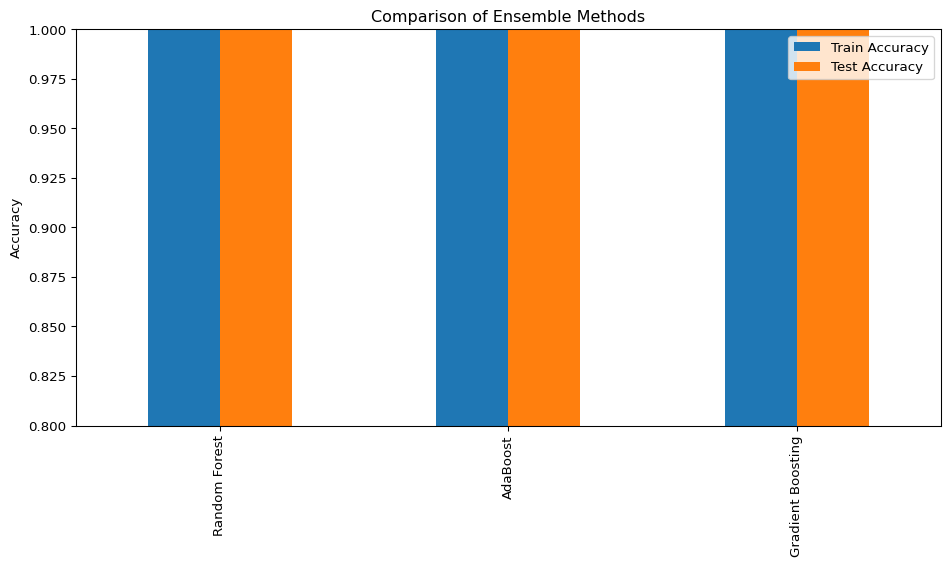
\includegraphics[keepaspectratio]{chapter6_files/figure-pdf/cell-8-output-3.png}}

\subsection{Bagging vs.~Boosting}\label{bagging-vs.-boosting}

\subsubsection{Bagging (Random Forest)}\label{bagging-random-forest}

\begin{itemize}
\tightlist
\item
  \textbf{Goal}: Reduce variance (overfitting)
\item
  \textbf{Training}: Parallel (trees are independent)
\item
  \textbf{Weighting}: Equal weight for all models
\item
  \textbf{Bias-Variance}: Primarily reduces variance
\item
  \textbf{Robustness}: Less prone to overfitting
\item
  \textbf{Speed}: Can be parallelized easily
\end{itemize}

\subsubsection{Boosting (Gradient
Boosting)}\label{boosting-gradient-boosting}

\begin{itemize}
\tightlist
\item
  \textbf{Goal}: Reduce bias and variance
\item
  \textbf{Training}: Sequential (each tree depends on previous trees)
\item
  \textbf{Weighting}: Different weights for different models
\item
  \textbf{Bias-Variance}: Reduces both bias and variance
\item
  \textbf{Robustness}: More prone to overfitting
\item
  \textbf{Speed}: Generally slower due to sequential nature
\end{itemize}

\subsection{Stacking}\label{stacking}

Stacking combines multiple models using a meta-learner:

\begin{enumerate}
\def\labelenumi{\arabic{enumi}.}
\tightlist
\item
  Train base models on the original dataset
\item
  Generate predictions from each base model
\item
  Use these predictions as features to train a meta-model
\item
  Final prediction is given by the meta-model
\end{enumerate}

\subsection{Choosing the Right Ensemble
Method}\label{choosing-the-right-ensemble-method}

The choice depends on the problem characteristics:

\begin{itemize}
\tightlist
\item
  \textbf{Random Forest}: Good default for most problems, especially
  with limited data
\item
  \textbf{Gradient Boosting}: When maximum performance is needed and you
  can tune hyperparameters
\item
  \textbf{AdaBoost}: Simple boosting algorithm, good for weak learners
\item
  \textbf{Stacking}: When you have diverse models and computational
  resources
\item
  \textbf{Voting}: Simple ensemble when you already have several good
  models
\end{itemize}

\subsection{Practical Considerations}\label{practical-considerations}

When implementing ensemble methods:

\begin{enumerate}
\def\labelenumi{\arabic{enumi}.}
\tightlist
\item
  \textbf{Computational Resources}: Boosting methods are generally more
  resource-intensive
\item
  \textbf{Model Complexity}: Simpler models may be preferred for
  production
\item
  \textbf{Interpretability Requirements}: Random forests offer better
  interpretability than boosting
\item
  \textbf{Dataset Size}: For small datasets, random forests may be more
  appropriate
\item
  \textbf{Noise Level}: For noisy data, bagging methods are more robust
\end{enumerate}

\section{Conclusion}\label{conclusion-1}

\begin{itemize}
\tightlist
\item
  Decision Trees provide interpretable models for both classification
  and regression
\item
  Ensemble methods like Random Forest and Gradient Boosting improve upon
  Decision Trees by combining multiple models
\item
  Random Forest reduces variance through bagging and random feature
  selection
\item
  Gradient Boosting reduces both bias and variance through sequential
  model building
\item
  Each method has strengths and weaknesses depending on the specific
  problem and dataset
\end{itemize}

\subsection{Key Takeaways}\label{key-takeaways}

\begin{enumerate}
\def\labelenumi{\arabic{enumi}.}
\tightlist
\item
  \textbf{No Free Lunch}: No single algorithm is best for all problems
\item
  \textbf{Bias-Variance Tradeoff}: Different ensemble methods address
  different aspects of model error
\item
  \textbf{Hyperparameter Tuning}: Proper tuning is crucial for optimal
  performance
\item
  \textbf{Interpretability vs.~Performance}: More complex ensembles
  usually offer better performance at the cost of interpretability
\item
  \textbf{Computational Considerations}: Training time and resource
  requirements vary significantly between methods
\end{enumerate}

\begin{Shaded}
\begin{Highlighting}[]
\CommentTok{\# Final comprehensive example: train models on different datasets and compare}

\ImportTok{from}\NormalTok{ sklearn.datasets }\ImportTok{import}\NormalTok{ load\_breast\_cancer, load\_wine}
\ImportTok{from}\NormalTok{ sklearn.preprocessing }\ImportTok{import}\NormalTok{ StandardScaler}

\NormalTok{datasets }\OperatorTok{=}\NormalTok{ \{}
    \StringTok{\textquotesingle{}Iris\textquotesingle{}}\NormalTok{: load\_iris(),}
    \StringTok{\textquotesingle{}Breast Cancer\textquotesingle{}}\NormalTok{: load\_breast\_cancer(),}
    \StringTok{\textquotesingle{}Wine\textquotesingle{}}\NormalTok{: load\_wine()}
\NormalTok{\}}

\NormalTok{results }\OperatorTok{=}\NormalTok{ []}

\ControlFlowTok{for}\NormalTok{ name, dataset }\KeywordTok{in}\NormalTok{ datasets.items():}
\NormalTok{    X, y }\OperatorTok{=}\NormalTok{ dataset.data, dataset.target}
    
    \CommentTok{\# Scale features}
\NormalTok{    scaler }\OperatorTok{=}\NormalTok{ StandardScaler()}
\NormalTok{    X }\OperatorTok{=}\NormalTok{ scaler.fit\_transform(X)}
    
    \CommentTok{\# Split data}
\NormalTok{    X\_train, X\_test, y\_train, y\_test }\OperatorTok{=}\NormalTok{ train\_test\_split(X, y, test\_size}\OperatorTok{=}\FloatTok{0.3}\NormalTok{, random\_state}\OperatorTok{=}\DecValTok{42}\NormalTok{)}
    
    \CommentTok{\# Train models}
\NormalTok{    dt }\OperatorTok{=}\NormalTok{ DecisionTreeClassifier(max\_depth}\OperatorTok{=}\DecValTok{4}\NormalTok{, random\_state}\OperatorTok{=}\DecValTok{42}\NormalTok{)}
\NormalTok{    rf }\OperatorTok{=}\NormalTok{ RandomForestClassifier(n\_estimators}\OperatorTok{=}\DecValTok{100}\NormalTok{, max\_depth}\OperatorTok{=}\DecValTok{4}\NormalTok{, random\_state}\OperatorTok{=}\DecValTok{42}\NormalTok{)}
\NormalTok{    gb }\OperatorTok{=}\NormalTok{ GradientBoostingClassifier(n\_estimators}\OperatorTok{=}\DecValTok{100}\NormalTok{, max\_depth}\OperatorTok{=}\DecValTok{3}\NormalTok{, random\_state}\OperatorTok{=}\DecValTok{42}\NormalTok{)}
    
\NormalTok{    models }\OperatorTok{=}\NormalTok{ \{}\StringTok{\textquotesingle{}Decision Tree\textquotesingle{}}\NormalTok{: dt, }\StringTok{\textquotesingle{}Random Forest\textquotesingle{}}\NormalTok{: rf, }\StringTok{\textquotesingle{}Gradient Boosting\textquotesingle{}}\NormalTok{: gb\}}
    
    \CommentTok{\# Evaluate}
    \ControlFlowTok{for}\NormalTok{ model\_name, model }\KeywordTok{in}\NormalTok{ models.items():}
\NormalTok{        model.fit(X\_train, y\_train)}
\NormalTok{        train\_acc }\OperatorTok{=}\NormalTok{ model.score(X\_train, y\_train)}
\NormalTok{        test\_acc }\OperatorTok{=}\NormalTok{ model.score(X\_test, y\_test)}
        
\NormalTok{        results.append(\{}
            \StringTok{\textquotesingle{}Dataset\textquotesingle{}}\NormalTok{: name,}
            \StringTok{\textquotesingle{}Model\textquotesingle{}}\NormalTok{: model\_name,}
            \StringTok{\textquotesingle{}Train Accuracy\textquotesingle{}}\NormalTok{: train\_acc,}
            \StringTok{\textquotesingle{}Test Accuracy\textquotesingle{}}\NormalTok{: test\_acc}
\NormalTok{        \})}

\CommentTok{\# Create DataFrame with results}
\NormalTok{final\_results }\OperatorTok{=}\NormalTok{ pd.DataFrame(results)}
\BuiltInTok{print}\NormalTok{(final\_results.pivot\_table(index}\OperatorTok{=}\StringTok{\textquotesingle{}Dataset\textquotesingle{}}\NormalTok{, columns}\OperatorTok{=}\StringTok{\textquotesingle{}Model\textquotesingle{}}\NormalTok{, values}\OperatorTok{=}\StringTok{\textquotesingle{}Test Accuracy\textquotesingle{}}\NormalTok{))}
\end{Highlighting}
\end{Shaded}

\begin{verbatim}
Model          Decision Tree  Gradient Boosting  Random Forest
Dataset                                                       
Breast Cancer       0.953216           0.959064        0.97076
Iris                1.000000           1.000000        1.00000
Wine                0.962963           0.907407        1.00000
\end{verbatim}

\subsection{Further Research
Directions}\label{further-research-directions}

\begin{itemize}
\tightlist
\item
  \textbf{Explainable AI}: Methods to interpret complex ensemble models
\item
  \textbf{Automatic Machine Learning (AutoML)}: Automating the selection
  and tuning of ensemble methods
\item
  \textbf{Deep Forest}: Combining deep learning concepts with random
  forests
\item
  \textbf{Online Learning}: Adapting ensemble methods for streaming data
\item
  \textbf{Imbalanced Learning}: Specialized ensemble techniques for
  imbalanced datasets
\end{itemize}

\bookmarksetup{startatroot}

\chapter{Support Vector Machines and Model
Evaluation}\label{support-vector-machines-and-model-evaluation}

\section{Support Vector Machine (SVM)}\label{support-vector-machine-svm}

Support Vector Machines (SVMs) are powerful supervised learning
algorithms used for both classification and regression tasks. Their
primary goal is to find the optimal hyperplane that maximizes the margin
between different classes.

\begin{Shaded}
\begin{Highlighting}[]
\ImportTok{import}\NormalTok{ numpy }\ImportTok{as}\NormalTok{ np}
\ImportTok{import}\NormalTok{ matplotlib.pyplot }\ImportTok{as}\NormalTok{ plt}
\ImportTok{from}\NormalTok{ sklearn }\ImportTok{import}\NormalTok{ svm, datasets}
\ImportTok{from}\NormalTok{ sklearn.model\_selection }\ImportTok{import}\NormalTok{ train\_test\_split}
\ImportTok{from}\NormalTok{ sklearn.preprocessing }\ImportTok{import}\NormalTok{ StandardScaler}
\end{Highlighting}
\end{Shaded}

\subsection{Key Concepts}\label{key-concepts}

\begin{itemize}
\tightlist
\item
  \textbf{Maximizes the margin} between classes to improve
  generalization
\item
  \textbf{Support vectors} are the data points closest to the decision
  boundary
\item
  \textbf{Decision boundary (hyperplane)} separates the classes
\item
  Based on optimization theory with learning bias derived from
  statistical learning theory
\end{itemize}

\subsubsection{Conceptual Understanding}\label{conceptual-understanding}

SVMs work by finding the hyperplane that creates the largest margin
between the two classes in the training data. This margin is defined as
the perpendicular distance between the decision boundary and the closest
data points from each class (the support vectors).

The mathematical objective of an SVM can be expressed as: - Maximize the
margin width (2/\textbar\textbar w\textbar\textbar) - Subject to
constraints that ensure no data points fall within the margin

The optimization problem becomes: - Minimize
(1/2)\textbar\textbar w\textbar\textbar² subject to y\_i(w·x\_i + b) ≥ 1
for all training points (x\_i, y\_i)

For non-linearly separable data, SVMs introduce ``slack variables'' (ξ)
that allow some points to violate the margin: - Minimize
(1/2)\textbar\textbar w\textbar\textbar² + C·Σξ\_i subject to
y\_i(w·x\_i + b) ≥ 1 - ξ\_i and ξ\_i ≥ 0

\begin{Shaded}
\begin{Highlighting}[]
\CommentTok{\# Load and prepare sample data}
\NormalTok{iris }\OperatorTok{=}\NormalTok{ datasets.load\_iris()}
\NormalTok{X }\OperatorTok{=}\NormalTok{ iris.data[:, :}\DecValTok{2}\NormalTok{]  }\CommentTok{\# Using first two features for visualization}
\NormalTok{y }\OperatorTok{=}\NormalTok{ iris.target}

\CommentTok{\# Only use two classes for binary classification example}
\NormalTok{X }\OperatorTok{=}\NormalTok{ X[y }\OperatorTok{!=} \DecValTok{2}\NormalTok{]}
\NormalTok{y }\OperatorTok{=}\NormalTok{ y[y }\OperatorTok{!=} \DecValTok{2}\NormalTok{]}

\CommentTok{\# Split data}
\NormalTok{X\_train, X\_test, y\_train, y\_test }\OperatorTok{=}\NormalTok{ train\_test\_split(X, y, test\_size}\OperatorTok{=}\FloatTok{0.3}\NormalTok{, random\_state}\OperatorTok{=}\DecValTok{42}\NormalTok{)}

\CommentTok{\# Standardize features}
\NormalTok{scaler }\OperatorTok{=}\NormalTok{ StandardScaler()}
\NormalTok{X\_train }\OperatorTok{=}\NormalTok{ scaler.fit\_transform(X\_train)}
\NormalTok{X\_test }\OperatorTok{=}\NormalTok{ scaler.transform(X\_test)}

\CommentTok{\# Create and train SVM classifier with linear kernel}
\NormalTok{clf }\OperatorTok{=}\NormalTok{ svm.SVC(kernel}\OperatorTok{=}\StringTok{\textquotesingle{}linear\textquotesingle{}}\NormalTok{, C}\OperatorTok{=}\FloatTok{1.0}\NormalTok{)}
\NormalTok{clf.fit(X\_train, y\_train)}

\CommentTok{\# Create a mesh to plot in}
\NormalTok{x\_min, x\_max }\OperatorTok{=}\NormalTok{ X\_train[:, }\DecValTok{0}\NormalTok{].}\BuiltInTok{min}\NormalTok{() }\OperatorTok{{-}} \DecValTok{1}\NormalTok{, X\_train[:, }\DecValTok{0}\NormalTok{].}\BuiltInTok{max}\NormalTok{() }\OperatorTok{+} \DecValTok{1}
\NormalTok{y\_min, y\_max }\OperatorTok{=}\NormalTok{ X\_train[:, }\DecValTok{1}\NormalTok{].}\BuiltInTok{min}\NormalTok{() }\OperatorTok{{-}} \DecValTok{1}\NormalTok{, X\_train[:, }\DecValTok{1}\NormalTok{].}\BuiltInTok{max}\NormalTok{() }\OperatorTok{+} \DecValTok{1}
\NormalTok{h }\OperatorTok{=} \FloatTok{0.02}  \CommentTok{\# Fixed step size for the mesh grid}
\NormalTok{xx, yy }\OperatorTok{=}\NormalTok{ np.meshgrid(np.arange(x\_min, x\_max, h),}
\NormalTok{                     np.arange(y\_min, y\_max, h))}

\CommentTok{\# Plot the decision boundary}
\NormalTok{Z }\OperatorTok{=}\NormalTok{ clf.predict(np.c\_[xx.ravel(), yy.ravel()])}
\NormalTok{Z }\OperatorTok{=}\NormalTok{ Z.reshape(xx.shape)}
\NormalTok{plt.contour(xx, yy, Z, colors}\OperatorTok{=}\StringTok{\textquotesingle{}k\textquotesingle{}}\NormalTok{, levels}\OperatorTok{=}\NormalTok{[}\OperatorTok{{-}}\DecValTok{1}\NormalTok{, }\DecValTok{0}\NormalTok{, }\DecValTok{1}\NormalTok{], linestyles}\OperatorTok{=}\NormalTok{[}\StringTok{\textquotesingle{}{-}{-}\textquotesingle{}}\NormalTok{, }\StringTok{\textquotesingle{}{-}\textquotesingle{}}\NormalTok{, }\StringTok{\textquotesingle{}{-}{-}\textquotesingle{}}\NormalTok{])}

\CommentTok{\# Plot the training points}
\NormalTok{plt.scatter(X\_train[:, }\DecValTok{0}\NormalTok{], X\_train[:, }\DecValTok{1}\NormalTok{], c}\OperatorTok{=}\NormalTok{y\_train, cmap}\OperatorTok{=}\NormalTok{plt.cm.Paired, }
\NormalTok{            edgecolors}\OperatorTok{=}\StringTok{\textquotesingle{}black\textquotesingle{}}\NormalTok{, s}\OperatorTok{=}\DecValTok{70}\NormalTok{)}

\CommentTok{\# Highlight the support vectors}
\NormalTok{plt.scatter(clf.support\_vectors\_[:, }\DecValTok{0}\NormalTok{], clf.support\_vectors\_[:, }\DecValTok{1}\NormalTok{], s}\OperatorTok{=}\DecValTok{100}\NormalTok{,}
\NormalTok{            linewidth}\OperatorTok{=}\DecValTok{1}\NormalTok{, facecolors}\OperatorTok{=}\StringTok{\textquotesingle{}none\textquotesingle{}}\NormalTok{, edgecolors}\OperatorTok{=}\StringTok{\textquotesingle{}k\textquotesingle{}}\NormalTok{)}

\NormalTok{plt.xlabel(}\StringTok{\textquotesingle{}Feature 1\textquotesingle{}}\NormalTok{)}
\NormalTok{plt.ylabel(}\StringTok{\textquotesingle{}Feature 2\textquotesingle{}}\NormalTok{)}
\NormalTok{plt.title(}\StringTok{\textquotesingle{}SVM Decision Boundary with Linear Kernel\textquotesingle{}}\NormalTok{)}
\NormalTok{plt.tight\_layout()}
\NormalTok{plt.show()}

\CommentTok{\# Print model accuracy}
\BuiltInTok{print}\NormalTok{(}\SpecialStringTok{f"Training accuracy: }\SpecialCharTok{\{}\NormalTok{clf}\SpecialCharTok{.}\NormalTok{score(X\_train, y\_train)}\SpecialCharTok{:.3f\}}\SpecialStringTok{"}\NormalTok{)}
\BuiltInTok{print}\NormalTok{(}\SpecialStringTok{f"Testing accuracy: }\SpecialCharTok{\{}\NormalTok{clf}\SpecialCharTok{.}\NormalTok{score(X\_test, y\_test)}\SpecialCharTok{:.3f\}}\SpecialStringTok{"}\NormalTok{)}
\end{Highlighting}
\end{Shaded}

\pandocbounded{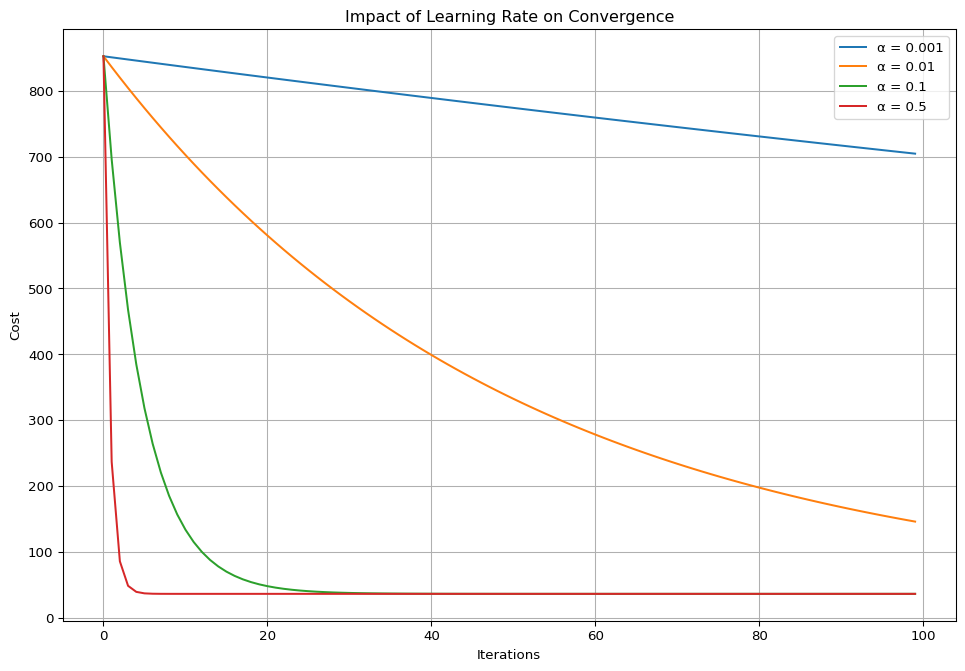
\includegraphics[keepaspectratio]{chapter6v2_files/figure-pdf/cell-3-output-1.png}}

\begin{verbatim}
Training accuracy: 0.986
Testing accuracy: 1.000
\end{verbatim}

\subsection{The Dual Problem and Support
Vectors}\label{the-dual-problem-and-support-vectors}

SVMs are often solved in their dual form using Lagrange multipliers,
which makes the kernel trick possible. The dual optimization problem
becomes:

\begin{itemize}
\tightlist
\item
  Maximize Σα\_i - (1/2)ΣΣα\_i·α\_j·y\_i·y\_j·K(x\_i, x\_j)
\item
  Subject to 0 ≤ α\_i ≤ C and Σα\_i·y\_i = 0
\end{itemize}

In this formulation: - Data points with α\_i \textgreater{} 0 are the
support vectors - Support vectors are the critical elements that define
the decision boundary - Only a subset of training points become support
vectors, making SVM memory-efficient

\subsection{SVM for Classification and
Regression}\label{svm-for-classification-and-regression}

SVMs can be used for both classification and regression tasks:

\subsubsection{SVM Classification (SVC)}\label{svm-classification-svc}

\begin{itemize}
\tightlist
\item
  \textbf{Binary Classification}: Finds the optimal hyperplane to
  separate two classes
\item
  \textbf{Multiclass Classification}: Uses strategies like one-vs-rest
  or one-vs-one
\item
  \textbf{Probabilistic Outputs}: Can be calibrated to provide
  probability estimates
\end{itemize}

\subsubsection{SVM Regression (SVR)}\label{svm-regression-svr}

\begin{itemize}
\tightlist
\item
  Predicts continuous values by finding a function that has at most ε
  deviation from the targets
\item
  Uses an ε-insensitive loss function: only errors greater than ε are
  penalized
\item
  Applies the same principles of margin maximization but for regression
\end{itemize}

\subsection{Non-linear Classification with
Kernels}\label{non-linear-classification-with-kernels}

When data isn't linearly separable in the original feature space, SVMs
use the \textbf{kernel trick} to implicitly map data into a
higher-dimensional space where linear separation becomes possible:

\begin{Shaded}
\begin{Highlighting}[]
\CommentTok{\# Compare different SVM kernels}
\NormalTok{kernels }\OperatorTok{=}\NormalTok{ [}\StringTok{\textquotesingle{}linear\textquotesingle{}}\NormalTok{, }\StringTok{\textquotesingle{}poly\textquotesingle{}}\NormalTok{, }\StringTok{\textquotesingle{}rbf\textquotesingle{}}\NormalTok{]}
\NormalTok{plt.figure(figsize}\OperatorTok{=}\NormalTok{(}\DecValTok{15}\NormalTok{, }\DecValTok{5}\NormalTok{))}

\ControlFlowTok{for}\NormalTok{ i, kernel }\KeywordTok{in} \BuiltInTok{enumerate}\NormalTok{(kernels):}
\NormalTok{    clf }\OperatorTok{=}\NormalTok{ svm.SVC(kernel}\OperatorTok{=}\NormalTok{kernel, gamma}\OperatorTok{=}\StringTok{\textquotesingle{}scale\textquotesingle{}}\NormalTok{)}
\NormalTok{    clf.fit(X\_train, y\_train)}
    
    \CommentTok{\# Plot the decision boundary}
\NormalTok{    plt.subplot(}\DecValTok{1}\NormalTok{, }\DecValTok{3}\NormalTok{, i}\OperatorTok{+}\DecValTok{1}\NormalTok{)}
    
    \CommentTok{\# Create a mesh to plot in}
\NormalTok{    x\_min, x\_max }\OperatorTok{=}\NormalTok{ X\_train[:, }\DecValTok{0}\NormalTok{].}\BuiltInTok{min}\NormalTok{() }\OperatorTok{{-}} \DecValTok{1}\NormalTok{, X\_train[:, }\DecValTok{0}\NormalTok{].}\BuiltInTok{max}\NormalTok{() }\OperatorTok{+} \DecValTok{1}
\NormalTok{    y\_min, y\_max }\OperatorTok{=}\NormalTok{ X\_train[:, }\DecValTok{1}\NormalTok{].}\BuiltInTok{min}\NormalTok{() }\OperatorTok{{-}} \DecValTok{1}\NormalTok{, X\_train[:, }\DecValTok{1}\NormalTok{].}\BuiltInTok{max}\NormalTok{() }\OperatorTok{+} \DecValTok{1}
\NormalTok{    xx, yy }\OperatorTok{=}\NormalTok{ np.meshgrid(np.arange(x\_min, x\_max, }\FloatTok{0.02}\NormalTok{),}
\NormalTok{                         np.arange(y\_min, y\_max, }\FloatTok{0.02}\NormalTok{))}
    
    \CommentTok{\# Plot the decision boundary}
\NormalTok{    Z }\OperatorTok{=}\NormalTok{ clf.predict(np.c\_[xx.ravel(), yy.ravel()])}
\NormalTok{    Z }\OperatorTok{=}\NormalTok{ Z.reshape(xx.shape)}
\NormalTok{    plt.contourf(xx, yy, Z, alpha}\OperatorTok{=}\FloatTok{0.8}\NormalTok{, cmap}\OperatorTok{=}\NormalTok{plt.cm.Paired)}
    
    \CommentTok{\# Plot the training points}
\NormalTok{    plt.scatter(X\_train[:, }\DecValTok{0}\NormalTok{], X\_train[:, }\DecValTok{1}\NormalTok{], c}\OperatorTok{=}\NormalTok{y\_train, cmap}\OperatorTok{=}\NormalTok{plt.cm.Paired, }
\NormalTok{                edgecolors}\OperatorTok{=}\StringTok{\textquotesingle{}black\textquotesingle{}}\NormalTok{)}
    
\NormalTok{    plt.xlabel(}\StringTok{\textquotesingle{}Feature 1\textquotesingle{}}\NormalTok{)}
\NormalTok{    plt.ylabel(}\StringTok{\textquotesingle{}Feature 2\textquotesingle{}}\NormalTok{)}
\NormalTok{    plt.title(}\SpecialStringTok{f\textquotesingle{}SVM with }\SpecialCharTok{\{}\NormalTok{kernel}\SpecialCharTok{.}\NormalTok{upper()}\SpecialCharTok{\}}\SpecialStringTok{ Kernel\textquotesingle{}}\NormalTok{)}
    
\NormalTok{    accuracy }\OperatorTok{=}\NormalTok{ clf.score(X\_test, y\_test)}
\NormalTok{    plt.text(x\_min }\OperatorTok{+} \FloatTok{0.2}\NormalTok{, y\_min }\OperatorTok{+} \FloatTok{0.2}\NormalTok{, }\SpecialStringTok{f\textquotesingle{}Accuracy: }\SpecialCharTok{\{}\NormalTok{accuracy}\SpecialCharTok{:.2f\}}\SpecialStringTok{\textquotesingle{}}\NormalTok{, }
\NormalTok{             bbox}\OperatorTok{=}\BuiltInTok{dict}\NormalTok{(facecolor}\OperatorTok{=}\StringTok{\textquotesingle{}white\textquotesingle{}}\NormalTok{, alpha}\OperatorTok{=}\FloatTok{0.5}\NormalTok{))}

\NormalTok{plt.tight\_layout()}
\NormalTok{plt.show()}
\end{Highlighting}
\end{Shaded}

\pandocbounded{\includegraphics[keepaspectratio]{chapter6v2_files/figure-pdf/cell-4-output-1.png}}

\subsubsection{Understanding the Kernel
Trick}\label{understanding-the-kernel-trick}

The kernel trick works by computing the dot product between the
transformed data points without explicitly calculating the
transformation:

K(x, y) = φ(x)·φ(y)

Where: - K is the kernel function - φ is the transformation function to
a higher-dimensional space - x and y are data points in the original
space

This allows SVM to operate in the transformed space without the
computational burden of explicitly computing the transformation.

\subsubsection{Common Kernel Types}\label{common-kernel-types}

\begin{enumerate}
\def\labelenumi{\arabic{enumi}.}
\tightlist
\item
  \textbf{Linear kernel}: K(x, y) = x·y

  \begin{itemize}
  \tightlist
  \item
    Used when data is linearly separable
  \item
    Simplest kernel with fewest parameters
  \item
    Decision boundary is a straight line (2D) or hyperplane (higher
    dimensions)
  \end{itemize}
\item
  \textbf{Radial Basis Function (RBF) kernel}: K(x, y) =
  exp(-γ\textbar\textbar x-y\textbar\textbar²)

  \begin{itemize}
  \tightlist
  \item
    Effective for non-linear boundaries
  \item
    Creates decision regions that can be distinct islands
  \item
    γ controls the influence radius of each support vector
  \end{itemize}
\item
  \textbf{Polynomial kernel}: K(x, y) = (γx·y + r)\^{}d

  \begin{itemize}
  \tightlist
  \item
    Creates complex curved decision boundaries
  \item
    d is the polynomial degree
  \item
    Higher degrees create more complex boundaries but risk overfitting
  \end{itemize}
\item
  \textbf{Sigmoid kernel}: K(x, y) = tanh(γx·y + r)

  \begin{itemize}
  \tightlist
  \item
    Inspired by neural networks
  \item
    Creates decision boundaries similar to those of neural networks
  \end{itemize}
\end{enumerate}

\subsection{SVM Parameters}\label{svm-parameters}

\subsubsection{The Role of C (Regularization
Parameter)}\label{the-role-of-c-regularization-parameter}

The \texttt{C} parameter represents the trade-off between model
complexity and training error:

\begin{Shaded}
\begin{Highlighting}[]
\CommentTok{\# Explore the effect of C parameter}
\NormalTok{C\_values }\OperatorTok{=}\NormalTok{ [}\FloatTok{0.1}\NormalTok{, }\DecValTok{1}\NormalTok{, }\DecValTok{10}\NormalTok{, }\DecValTok{100}\NormalTok{]}
\NormalTok{plt.figure(figsize}\OperatorTok{=}\NormalTok{(}\DecValTok{15}\NormalTok{, }\DecValTok{10}\NormalTok{))}

\ControlFlowTok{for}\NormalTok{ i, C }\KeywordTok{in} \BuiltInTok{enumerate}\NormalTok{(C\_values):}
\NormalTok{    clf }\OperatorTok{=}\NormalTok{ svm.SVC(kernel}\OperatorTok{=}\StringTok{\textquotesingle{}rbf\textquotesingle{}}\NormalTok{, C}\OperatorTok{=}\NormalTok{C, gamma}\OperatorTok{=}\StringTok{\textquotesingle{}scale\textquotesingle{}}\NormalTok{)}
\NormalTok{    clf.fit(X\_train, y\_train)}
    
    \CommentTok{\# Plot the decision boundary}
\NormalTok{    plt.subplot(}\DecValTok{2}\NormalTok{, }\DecValTok{2}\NormalTok{, i}\OperatorTok{+}\DecValTok{1}\NormalTok{)}
    
    \CommentTok{\# Create a mesh to plot in}
\NormalTok{    x\_min, x\_max }\OperatorTok{=}\NormalTok{ X\_train[:, }\DecValTok{0}\NormalTok{].}\BuiltInTok{min}\NormalTok{() }\OperatorTok{{-}} \DecValTok{1}\NormalTok{, X\_train[:, }\DecValTok{0}\NormalTok{].}\BuiltInTok{max}\NormalTok{() }\OperatorTok{+} \DecValTok{1}
\NormalTok{    y\_min, y\_max }\OperatorTok{=}\NormalTok{ X\_train[:, }\DecValTok{1}\NormalTok{].}\BuiltInTok{min}\NormalTok{() }\OperatorTok{{-}} \DecValTok{1}\NormalTok{, X\_train[:, }\DecValTok{1}\NormalTok{].}\BuiltInTok{max}\NormalTok{() }\OperatorTok{+} \DecValTok{1}
\NormalTok{    xx, yy }\OperatorTok{=}\NormalTok{ np.meshgrid(np.arange(x\_min, x\_max, }\FloatTok{0.02}\NormalTok{),}
\NormalTok{                         np.arange(y\_min, y\_max, }\FloatTok{0.02}\NormalTok{))}
    
    \CommentTok{\# Plot the decision boundary}
\NormalTok{    Z }\OperatorTok{=}\NormalTok{ clf.predict(np.c\_[xx.ravel(), yy.ravel()])}
\NormalTok{    Z }\OperatorTok{=}\NormalTok{ Z.reshape(xx.shape)}
\NormalTok{    plt.contourf(xx, yy, Z, alpha}\OperatorTok{=}\FloatTok{0.8}\NormalTok{, cmap}\OperatorTok{=}\NormalTok{plt.cm.Paired)}
    
    \CommentTok{\# Plot the training points}
\NormalTok{    plt.scatter(X\_train[:, }\DecValTok{0}\NormalTok{], X\_train[:, }\DecValTok{1}\NormalTok{], c}\OperatorTok{=}\NormalTok{y\_train, cmap}\OperatorTok{=}\NormalTok{plt.cm.Paired, }
\NormalTok{                edgecolors}\OperatorTok{=}\StringTok{\textquotesingle{}black\textquotesingle{}}\NormalTok{)}
    
\NormalTok{    plt.xlabel(}\StringTok{\textquotesingle{}Feature 1\textquotesingle{}}\NormalTok{)}
\NormalTok{    plt.ylabel(}\StringTok{\textquotesingle{}Feature 2\textquotesingle{}}\NormalTok{)}
\NormalTok{    plt.title(}\SpecialStringTok{f\textquotesingle{}SVM with C=}\SpecialCharTok{\{}\NormalTok{C}\SpecialCharTok{\}}\SpecialStringTok{\textquotesingle{}}\NormalTok{)}
    
\NormalTok{    train\_accuracy }\OperatorTok{=}\NormalTok{ clf.score(X\_train, y\_train)}
\NormalTok{    test\_accuracy }\OperatorTok{=}\NormalTok{ clf.score(X\_test, y\_test)}
\NormalTok{    plt.text(x\_min }\OperatorTok{+} \FloatTok{0.2}\NormalTok{, y\_min }\OperatorTok{+} \FloatTok{0.5}\NormalTok{, }
             \SpecialStringTok{f\textquotesingle{}Train Acc: }\SpecialCharTok{\{}\NormalTok{train\_accuracy}\SpecialCharTok{:.2f\}}\CharTok{\textbackslash{}n}\SpecialStringTok{Test Acc: }\SpecialCharTok{\{}\NormalTok{test\_accuracy}\SpecialCharTok{:.2f\}}\SpecialStringTok{\textquotesingle{}}\NormalTok{, }
\NormalTok{             bbox}\OperatorTok{=}\BuiltInTok{dict}\NormalTok{(facecolor}\OperatorTok{=}\StringTok{\textquotesingle{}white\textquotesingle{}}\NormalTok{, alpha}\OperatorTok{=}\FloatTok{0.5}\NormalTok{))}

\NormalTok{plt.tight\_layout()}
\NormalTok{plt.show()}
\end{Highlighting}
\end{Shaded}

\pandocbounded{\includegraphics[keepaspectratio]{chapter6v2_files/figure-pdf/cell-5-output-1.png}}

\begin{itemize}
\tightlist
\item
  \textbf{Large C}: Penalizes misclassifications heavily

  \begin{itemize}
  \tightlist
  \item
    Creates a smaller-margin hyperplane that attempts to classify all
    training examples correctly
  \item
    May lead to overfitting by creating complex decision boundaries
  \item
    More support vectors are typically used
  \end{itemize}
\item
  \textbf{Small C}: Allows more misclassifications

  \begin{itemize}
  \tightlist
  \item
    Creates a wider margin that may misclassify more training points
  \item
    Produces simpler, more generalized models
  \item
    Fewer support vectors are typically used
  \end{itemize}
\end{itemize}

\subsubsection{The Role of Gamma (Kernel
Coefficient)}\label{the-role-of-gamma-kernel-coefficient}

For RBF, polynomial, and sigmoid kernels, the \texttt{gamma} parameter
defines how far the influence of a single training example reaches:

\begin{itemize}
\tightlist
\item
  \textbf{Large gamma}: Results in a decision boundary that closely
  follows individual training examples

  \begin{itemize}
  \tightlist
  \item
    May lead to overfitting as the model becomes too specialized to
    training data
  \item
    Creates more complex, tightly curved decision boundaries
  \end{itemize}
\item
  \textbf{Small gamma}: Gives points far away from the decision boundary
  more influence

  \begin{itemize}
  \tightlist
  \item
    Creates smoother, simpler decision boundaries
  \item
    May lead to underfitting if too small
  \end{itemize}
\end{itemize}

\subsection{Strengths and Weaknesses of
SVM}\label{strengths-and-weaknesses-of-svm}

\subsubsection{Strengths}\label{strengths}

\begin{itemize}
\tightlist
\item
  \textbf{No Local Minima}: The optimization problem is convex, ensuring
  a globally optimized solution
\item
  \textbf{Memory Efficiency}: Only support vectors are needed to define
  the decision boundary
\item
  \textbf{Versatility}: Effective with both linear and non-linear data
  via different kernels
\item
  \textbf{Robustness}: Less prone to overfitting in high-dimensional
  spaces
\item
  \textbf{Theoretical Guarantees}: Based on statistical learning theory
  with solid mathematical foundations
\end{itemize}

\subsubsection{Weaknesses}\label{weaknesses}

\begin{itemize}
\tightlist
\item
  \textbf{Computationally Intensive}: For large datasets, especially
  with non-linear kernels (O(n²) to O(n³) complexity)
\item
  \textbf{Sensitive to Parameters}: Performance depends on appropriate
  kernel and parameter selection
\item
  \textbf{Black Box Nature}: Limited interpretability compared to
  simpler models
\item
  \textbf{Not Directly Probabilistic}: Requires additional calibration
  for probability outputs
\item
  \textbf{Struggles with Highly Imbalanced Data}: Without adjustment,
  tends to favor the majority class
\end{itemize}

\subsection{Practical Example: Full Iris
Dataset}\label{practical-example-full-iris-dataset}

\begin{Shaded}
\begin{Highlighting}[]
\CommentTok{\# Use all features and classes from the Iris dataset}
\NormalTok{iris }\OperatorTok{=}\NormalTok{ datasets.load\_iris()}
\NormalTok{X }\OperatorTok{=}\NormalTok{ iris.data}
\NormalTok{y }\OperatorTok{=}\NormalTok{ iris.target}

\CommentTok{\# Split data}
\NormalTok{X\_train, X\_test, y\_train, y\_test }\OperatorTok{=}\NormalTok{ train\_test\_split(X, y, test\_size}\OperatorTok{=}\FloatTok{0.3}\NormalTok{, random\_state}\OperatorTok{=}\DecValTok{42}\NormalTok{)}

\CommentTok{\# Standardize features}
\NormalTok{scaler }\OperatorTok{=}\NormalTok{ StandardScaler()}
\NormalTok{X\_train }\OperatorTok{=}\NormalTok{ scaler.fit\_transform(X\_train)}
\NormalTok{X\_test }\OperatorTok{=}\NormalTok{ scaler.transform(X\_test)}

\CommentTok{\# Create and train SVM classifier}
\NormalTok{clf }\OperatorTok{=}\NormalTok{ svm.SVC(kernel}\OperatorTok{=}\StringTok{\textquotesingle{}rbf\textquotesingle{}}\NormalTok{, C}\OperatorTok{=}\FloatTok{1.0}\NormalTok{, gamma}\OperatorTok{=}\StringTok{\textquotesingle{}scale\textquotesingle{}}\NormalTok{)}
\NormalTok{clf.fit(X\_train, y\_train)}

\CommentTok{\# Make predictions}
\NormalTok{y\_pred }\OperatorTok{=}\NormalTok{ clf.predict(X\_test)}

\CommentTok{\# Print performance metrics}
\ImportTok{from}\NormalTok{ sklearn.metrics }\ImportTok{import}\NormalTok{ classification\_report, confusion\_matrix}
\BuiltInTok{print}\NormalTok{(}\StringTok{"Confusion Matrix:"}\NormalTok{)}
\BuiltInTok{print}\NormalTok{(confusion\_matrix(y\_test, y\_pred))}
\BuiltInTok{print}\NormalTok{(}\StringTok{"}\CharTok{\textbackslash{}n}\StringTok{Classification Report:"}\NormalTok{)}
\BuiltInTok{print}\NormalTok{(classification\_report(y\_test, y\_pred, target\_names}\OperatorTok{=}\NormalTok{iris.target\_names))}
\end{Highlighting}
\end{Shaded}

\begin{verbatim}
Confusion Matrix:
[[19  0  0]
 [ 0 13  0]
 [ 0  0 13]]

Classification Report:
              precision    recall  f1-score   support

      setosa       1.00      1.00      1.00        19
  versicolor       1.00      1.00      1.00        13
   virginica       1.00      1.00      1.00        13

    accuracy                           1.00        45
   macro avg       1.00      1.00      1.00        45
weighted avg       1.00      1.00      1.00        45
\end{verbatim}

\section{Performance Metrics in Machine
Learning}\label{performance-metrics-in-machine-learning}

Performance metrics are crucial for evaluating how well machine learning
models perform. The choice of metric depends on the type of task
(classification or regression) and the specific problem requirements.

\subsection{Classification Metrics}\label{classification-metrics}

\begin{Shaded}
\begin{Highlighting}[]
\ImportTok{import}\NormalTok{ pandas }\ImportTok{as}\NormalTok{ pd}
\ImportTok{from}\NormalTok{ sklearn.metrics }\ImportTok{import}\NormalTok{ accuracy\_score, precision\_score, recall\_score, f1\_score}
\ImportTok{from}\NormalTok{ sklearn.metrics }\ImportTok{import}\NormalTok{ confusion\_matrix, roc\_curve, auc, precision\_recall\_curve}

\CommentTok{\# Function to calculate and display all classification metrics}
\KeywordTok{def}\NormalTok{ evaluate\_classification(y\_true, y\_pred, y\_scores}\OperatorTok{=}\VariableTok{None}\NormalTok{):}
    \CommentTok{"""}
\CommentTok{    Calculate classification metrics}
\CommentTok{    }
\CommentTok{    Parameters:}
\CommentTok{    y\_true: True labels}
\CommentTok{    y\_pred: Predicted labels}
\CommentTok{    y\_scores: Predicted probabilities (for ROC and PR curves)}
\CommentTok{    """}
    \CommentTok{\# Basic metrics}
\NormalTok{    accuracy }\OperatorTok{=}\NormalTok{ accuracy\_score(y\_true, y\_pred)}
    
    \CommentTok{\# For multi{-}class, we use \textquotesingle{}macro\textquotesingle{} average}
\NormalTok{    precision }\OperatorTok{=}\NormalTok{ precision\_score(y\_true, y\_pred, average}\OperatorTok{=}\StringTok{\textquotesingle{}macro\textquotesingle{}}\NormalTok{)}
\NormalTok{    recall }\OperatorTok{=}\NormalTok{ recall\_score(y\_true, y\_pred, average}\OperatorTok{=}\StringTok{\textquotesingle{}macro\textquotesingle{}}\NormalTok{)}
\NormalTok{    f1 }\OperatorTok{=}\NormalTok{ f1\_score(y\_true, y\_pred, average}\OperatorTok{=}\StringTok{\textquotesingle{}macro\textquotesingle{}}\NormalTok{)}
    
    \BuiltInTok{print}\NormalTok{(}\SpecialStringTok{f"Accuracy: }\SpecialCharTok{\{}\NormalTok{accuracy}\SpecialCharTok{:.4f\}}\SpecialStringTok{"}\NormalTok{)}
    \BuiltInTok{print}\NormalTok{(}\SpecialStringTok{f"Precision: }\SpecialCharTok{\{}\NormalTok{precision}\SpecialCharTok{:.4f\}}\SpecialStringTok{"}\NormalTok{)}
    \BuiltInTok{print}\NormalTok{(}\SpecialStringTok{f"Recall: }\SpecialCharTok{\{}\NormalTok{recall}\SpecialCharTok{:.4f\}}\SpecialStringTok{"}\NormalTok{)}
    \BuiltInTok{print}\NormalTok{(}\SpecialStringTok{f"F1 Score: }\SpecialCharTok{\{}\NormalTok{f1}\SpecialCharTok{:.4f\}}\SpecialStringTok{"}\NormalTok{)}
    
    \CommentTok{\# Confusion Matrix}
\NormalTok{    cm }\OperatorTok{=}\NormalTok{ confusion\_matrix(y\_true, y\_pred)}
\NormalTok{    plt.figure(figsize}\OperatorTok{=}\NormalTok{(}\DecValTok{8}\NormalTok{, }\DecValTok{6}\NormalTok{))}
\NormalTok{    plt.imshow(cm, interpolation}\OperatorTok{=}\StringTok{\textquotesingle{}nearest\textquotesingle{}}\NormalTok{, cmap}\OperatorTok{=}\NormalTok{plt.cm.Blues)}
\NormalTok{    plt.title(}\StringTok{\textquotesingle{}Confusion Matrix\textquotesingle{}}\NormalTok{)}
\NormalTok{    plt.colorbar()}
    
\NormalTok{    classes }\OperatorTok{=}\NormalTok{ np.unique(y\_true)}
\NormalTok{    tick\_marks }\OperatorTok{=}\NormalTok{ np.arange(}\BuiltInTok{len}\NormalTok{(classes))}
\NormalTok{    plt.xticks(tick\_marks, classes)}
\NormalTok{    plt.yticks(tick\_marks, classes)}
    
    \CommentTok{\# Add text annotations}
\NormalTok{    thresh }\OperatorTok{=}\NormalTok{ cm.}\BuiltInTok{max}\NormalTok{() }\OperatorTok{/} \DecValTok{2}
    \ControlFlowTok{for}\NormalTok{ i }\KeywordTok{in} \BuiltInTok{range}\NormalTok{(cm.shape[}\DecValTok{0}\NormalTok{]):}
        \ControlFlowTok{for}\NormalTok{ j }\KeywordTok{in} \BuiltInTok{range}\NormalTok{(cm.shape[}\DecValTok{1}\NormalTok{]):}
\NormalTok{            plt.text(j, i, }\BuiltInTok{format}\NormalTok{(cm[i, j], }\StringTok{\textquotesingle{}d\textquotesingle{}}\NormalTok{),}
\NormalTok{                     horizontalalignment}\OperatorTok{=}\StringTok{"center"}\NormalTok{,}
\NormalTok{                     color}\OperatorTok{=}\StringTok{"white"} \ControlFlowTok{if}\NormalTok{ cm[i, j] }\OperatorTok{\textgreater{}}\NormalTok{ thresh }\ControlFlowTok{else} \StringTok{"black"}\NormalTok{)}
    
\NormalTok{    plt.ylabel(}\StringTok{\textquotesingle{}True label\textquotesingle{}}\NormalTok{)}
\NormalTok{    plt.xlabel(}\StringTok{\textquotesingle{}Predicted label\textquotesingle{}}\NormalTok{)}
\NormalTok{    plt.tight\_layout()}
\NormalTok{    plt.show()}
    
    \CommentTok{\# If we have probability scores, calculate ROC curve (for binary classification)}
    \ControlFlowTok{if}\NormalTok{ y\_scores }\KeywordTok{is} \KeywordTok{not} \VariableTok{None} \KeywordTok{and} \BuiltInTok{len}\NormalTok{(np.unique(y\_true)) }\OperatorTok{==} \DecValTok{2}\NormalTok{:}
        \CommentTok{\# ROC Curve}
\NormalTok{        fpr, tpr, \_ }\OperatorTok{=}\NormalTok{ roc\_curve(y\_true, y\_scores)}
\NormalTok{        roc\_auc }\OperatorTok{=}\NormalTok{ auc(fpr, tpr)}
        
\NormalTok{        plt.figure(figsize}\OperatorTok{=}\NormalTok{(}\DecValTok{8}\NormalTok{, }\DecValTok{6}\NormalTok{))}
\NormalTok{        plt.plot(fpr, tpr, color}\OperatorTok{=}\StringTok{\textquotesingle{}darkorange\textquotesingle{}}\NormalTok{, lw}\OperatorTok{=}\DecValTok{2}\NormalTok{, }
\NormalTok{                 label}\OperatorTok{=}\SpecialStringTok{f\textquotesingle{}ROC curve (area = }\SpecialCharTok{\{}\NormalTok{roc\_auc}\SpecialCharTok{:.2f\}}\SpecialStringTok{)\textquotesingle{}}\NormalTok{)}
\NormalTok{        plt.plot([}\DecValTok{0}\NormalTok{, }\DecValTok{1}\NormalTok{], [}\DecValTok{0}\NormalTok{, }\DecValTok{1}\NormalTok{], color}\OperatorTok{=}\StringTok{\textquotesingle{}navy\textquotesingle{}}\NormalTok{, lw}\OperatorTok{=}\DecValTok{2}\NormalTok{, linestyle}\OperatorTok{=}\StringTok{\textquotesingle{}{-}{-}\textquotesingle{}}\NormalTok{)}
\NormalTok{        plt.xlim([}\FloatTok{0.0}\NormalTok{, }\FloatTok{1.0}\NormalTok{])}
\NormalTok{        plt.ylim([}\FloatTok{0.0}\NormalTok{, }\FloatTok{1.05}\NormalTok{])}
\NormalTok{        plt.xlabel(}\StringTok{\textquotesingle{}False Positive Rate\textquotesingle{}}\NormalTok{)}
\NormalTok{        plt.ylabel(}\StringTok{\textquotesingle{}True Positive Rate\textquotesingle{}}\NormalTok{)}
\NormalTok{        plt.title(}\StringTok{\textquotesingle{}Receiver Operating Characteristic (ROC) Curve\textquotesingle{}}\NormalTok{)}
\NormalTok{        plt.legend(loc}\OperatorTok{=}\StringTok{"lower right"}\NormalTok{)}
\NormalTok{        plt.show()}
        
        \CommentTok{\# Precision{-}Recall Curve}
\NormalTok{        precision, recall, \_ }\OperatorTok{=}\NormalTok{ precision\_recall\_curve(y\_true, y\_scores)}
        
\NormalTok{        plt.figure(figsize}\OperatorTok{=}\NormalTok{(}\DecValTok{8}\NormalTok{, }\DecValTok{6}\NormalTok{))}
\NormalTok{        plt.plot(recall, precision, color}\OperatorTok{=}\StringTok{\textquotesingle{}blue\textquotesingle{}}\NormalTok{, lw}\OperatorTok{=}\DecValTok{2}\NormalTok{)}
\NormalTok{        plt.xlabel(}\StringTok{\textquotesingle{}Recall\textquotesingle{}}\NormalTok{)}
\NormalTok{        plt.ylabel(}\StringTok{\textquotesingle{}Precision\textquotesingle{}}\NormalTok{)}
\NormalTok{        plt.title(}\StringTok{\textquotesingle{}Precision{-}Recall Curve\textquotesingle{}}\NormalTok{)}
\NormalTok{        plt.xlim([}\FloatTok{0.0}\NormalTok{, }\FloatTok{1.0}\NormalTok{])}
\NormalTok{        plt.ylim([}\FloatTok{0.0}\NormalTok{, }\FloatTok{1.05}\NormalTok{])}
\NormalTok{        plt.show()}

\CommentTok{\# Example using our SVM model from earlier}
\CommentTok{\# For binary classification demo}
\ImportTok{from}\NormalTok{ sklearn.svm }\ImportTok{import}\NormalTok{ SVC}

\CommentTok{\# Create binary classification problem}
\NormalTok{binary\_X }\OperatorTok{=}\NormalTok{ iris.data[iris.target }\OperatorTok{!=} \DecValTok{2}\NormalTok{]}
\NormalTok{binary\_y }\OperatorTok{=}\NormalTok{ iris.target[iris.target }\OperatorTok{!=} \DecValTok{2}\NormalTok{]}

\NormalTok{X\_train, X\_test, y\_train, y\_test }\OperatorTok{=}\NormalTok{ train\_test\_split(binary\_X, binary\_y, }
\NormalTok{                                                    test\_size}\OperatorTok{=}\FloatTok{0.3}\NormalTok{, random\_state}\OperatorTok{=}\DecValTok{42}\NormalTok{)}

\CommentTok{\# Create SVM model with probability output}
\NormalTok{binary\_clf }\OperatorTok{=}\NormalTok{ SVC(kernel}\OperatorTok{=}\StringTok{\textquotesingle{}rbf\textquotesingle{}}\NormalTok{, probability}\OperatorTok{=}\VariableTok{True}\NormalTok{)}
\NormalTok{binary\_clf.fit(X\_train, y\_train)}

\CommentTok{\# Get predictions and probability scores}
\NormalTok{y\_pred }\OperatorTok{=}\NormalTok{ binary\_clf.predict(X\_test)}
\NormalTok{y\_scores }\OperatorTok{=}\NormalTok{ binary\_clf.predict\_proba(X\_test)[:, }\DecValTok{1}\NormalTok{]  }\CommentTok{\# Probability of class 1}

\BuiltInTok{print}\NormalTok{(}\StringTok{"Binary Classification Metrics:"}\NormalTok{)}
\NormalTok{evaluate\_classification(y\_test, y\_pred, y\_scores)}
\end{Highlighting}
\end{Shaded}

\begin{verbatim}
Binary Classification Metrics:
Accuracy: 1.0000
Precision: 1.0000
Recall: 1.0000
F1 Score: 1.0000
\end{verbatim}

\pandocbounded{\includegraphics[keepaspectratio]{chapter6v2_files/figure-pdf/cell-7-output-2.png}}

\pandocbounded{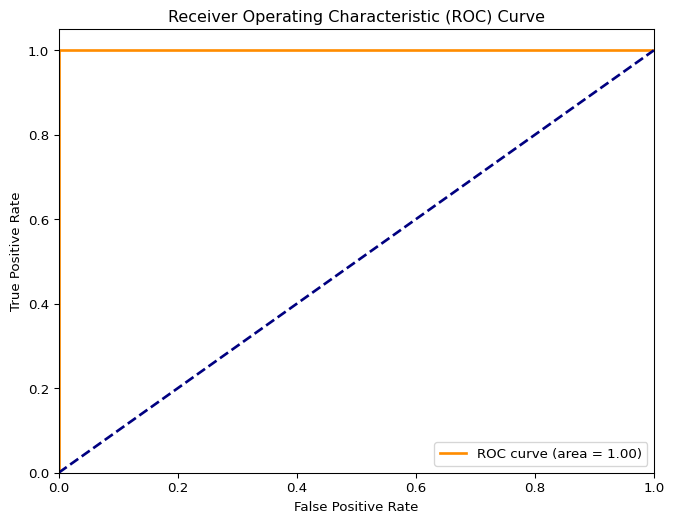
\includegraphics[keepaspectratio]{chapter6v2_files/figure-pdf/cell-7-output-3.png}}

\pandocbounded{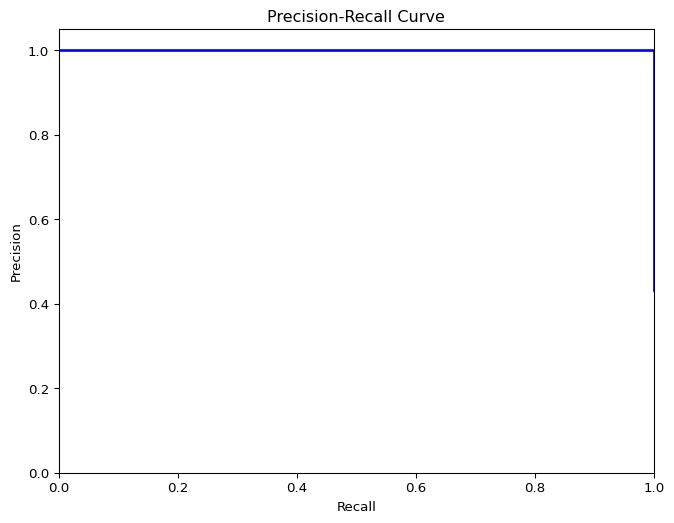
\includegraphics[keepaspectratio]{chapter6v2_files/figure-pdf/cell-7-output-4.png}}

\subsubsection{1. Accuracy}\label{accuracy}

Measures the proportion of correctly classified instances: - Formula:
Accuracy = (TP + TN) / (TP + TN + FP + FN) - Simple and intuitive, but
can be misleading for imbalanced datasets - Example: In a dataset with
95\% negative samples, a model that always predicts ``negative'' would
have 95\% accuracy despite being useless

\subsubsection{2. Precision}\label{precision}

Measures how many predicted positives were actually positive: - Formula:
Precision = TP / (TP + FP) - Answers: ``Of all instances predicted as
positive, how many were actually positive?'' - Important when false
positives are costly (e.g., spam detection, medical diagnosis) - High
precision indicates low false positive rate

\subsubsection{3. Recall (Sensitivity or True Positive
Rate)}\label{recall-sensitivity-or-true-positive-rate}

Measures how many actual positives were correctly predicted: - Formula:
Recall = TP / (TP + FN) - Answers: ``Of all actual positive instances,
how many did we correctly identify?'' - Important when false negatives
are costly (e.g., disease screening, fraud detection) - High recall
indicates low false negative rate

\subsubsection{4. F1 Score}\label{f1-score}

Harmonic mean of precision and recall: - Formula: F1 Score = 2 ×
(Precision × Recall) / (Precision + Recall) - Balances precision and
recall into a single metric - Particularly useful for imbalanced
datasets - F1 Score is low if either precision or recall is low

\subsubsection{5. Confusion Matrix}\label{confusion-matrix}

Tabular representation of actual vs.~predicted values: - True Positives
(TP): Correctly predicted positives - True Negatives (TN): Correctly
predicted negatives - False Positives (FP): Incorrectly predicted
positives (Type I error) - False Negatives (FN): Incorrectly predicted
negatives (Type II error)

The confusion matrix provides a comprehensive view of model performance
and serves as the basis for calculating most classification metrics.

\subsection{Understanding ROC and Precision-Recall
Curves}\label{understanding-roc-and-precision-recall-curves}

\subsubsection{ROC Curve (Receiver Operating
Characteristic)}\label{roc-curve-receiver-operating-characteristic}

The ROC curve plots the True Positive Rate (TPR) against the False
Positive Rate (FPR) at various classification thresholds:

\begin{Shaded}
\begin{Highlighting}[]
\CommentTok{\# ROC Curve across different classification thresholds}
\ImportTok{from}\NormalTok{ sklearn.metrics }\ImportTok{import}\NormalTok{ roc\_curve, auc}
\ImportTok{from}\NormalTok{ sklearn.linear\_model }\ImportTok{import}\NormalTok{ LogisticRegression}
\ImportTok{from}\NormalTok{ sklearn.ensemble }\ImportTok{import}\NormalTok{ RandomForestClassifier}

\CommentTok{\# Train multiple classifiers on the same binary dataset}
\NormalTok{classifiers }\OperatorTok{=}\NormalTok{ \{}
    \StringTok{\textquotesingle{}SVM\textquotesingle{}}\NormalTok{: SVC(kernel}\OperatorTok{=}\StringTok{\textquotesingle{}rbf\textquotesingle{}}\NormalTok{, probability}\OperatorTok{=}\VariableTok{True}\NormalTok{, random\_state}\OperatorTok{=}\DecValTok{42}\NormalTok{),}
    \StringTok{\textquotesingle{}Logistic Regression\textquotesingle{}}\NormalTok{: LogisticRegression(random\_state}\OperatorTok{=}\DecValTok{42}\NormalTok{),}
    \StringTok{\textquotesingle{}Random Forest\textquotesingle{}}\NormalTok{: RandomForestClassifier(random\_state}\OperatorTok{=}\DecValTok{42}\NormalTok{)}
\NormalTok{\}}

\NormalTok{plt.figure(figsize}\OperatorTok{=}\NormalTok{(}\DecValTok{10}\NormalTok{, }\DecValTok{8}\NormalTok{))}

\CommentTok{\# Plot ROC for each classifier}
\ControlFlowTok{for}\NormalTok{ name, clf }\KeywordTok{in}\NormalTok{ classifiers.items():}
\NormalTok{    clf.fit(X\_train, y\_train)}
\NormalTok{    y\_scores }\OperatorTok{=}\NormalTok{ clf.predict\_proba(X\_test)[:, }\DecValTok{1}\NormalTok{]}
    
\NormalTok{    fpr, tpr, \_ }\OperatorTok{=}\NormalTok{ roc\_curve(y\_test, y\_scores)}
\NormalTok{    roc\_auc }\OperatorTok{=}\NormalTok{ auc(fpr, tpr)}
    
\NormalTok{    plt.plot(fpr, tpr, lw}\OperatorTok{=}\DecValTok{2}\NormalTok{, label}\OperatorTok{=}\SpecialStringTok{f\textquotesingle{}}\SpecialCharTok{\{}\NormalTok{name}\SpecialCharTok{\}}\SpecialStringTok{ (AUC = }\SpecialCharTok{\{}\NormalTok{roc\_auc}\SpecialCharTok{:.2f\}}\SpecialStringTok{)\textquotesingle{}}\NormalTok{)}

\CommentTok{\# Plot the random guessing line}
\NormalTok{plt.plot([}\DecValTok{0}\NormalTok{, }\DecValTok{1}\NormalTok{], [}\DecValTok{0}\NormalTok{, }\DecValTok{1}\NormalTok{], color}\OperatorTok{=}\StringTok{\textquotesingle{}navy\textquotesingle{}}\NormalTok{, lw}\OperatorTok{=}\DecValTok{2}\NormalTok{, linestyle}\OperatorTok{=}\StringTok{\textquotesingle{}{-}{-}\textquotesingle{}}\NormalTok{, label}\OperatorTok{=}\StringTok{\textquotesingle{}Random Guessing\textquotesingle{}}\NormalTok{)}

\NormalTok{plt.xlim([}\FloatTok{0.0}\NormalTok{, }\FloatTok{1.0}\NormalTok{])}
\NormalTok{plt.ylim([}\FloatTok{0.0}\NormalTok{, }\FloatTok{1.05}\NormalTok{])}
\NormalTok{plt.xlabel(}\StringTok{\textquotesingle{}False Positive Rate\textquotesingle{}}\NormalTok{)}
\NormalTok{plt.ylabel(}\StringTok{\textquotesingle{}True Positive Rate\textquotesingle{}}\NormalTok{)}
\NormalTok{plt.title(}\StringTok{\textquotesingle{}ROC Curves for Different Classifiers\textquotesingle{}}\NormalTok{)}
\NormalTok{plt.legend(loc}\OperatorTok{=}\StringTok{"lower right"}\NormalTok{)}
\NormalTok{plt.grid(}\VariableTok{True}\NormalTok{)}
\NormalTok{plt.show()}
\end{Highlighting}
\end{Shaded}

\pandocbounded{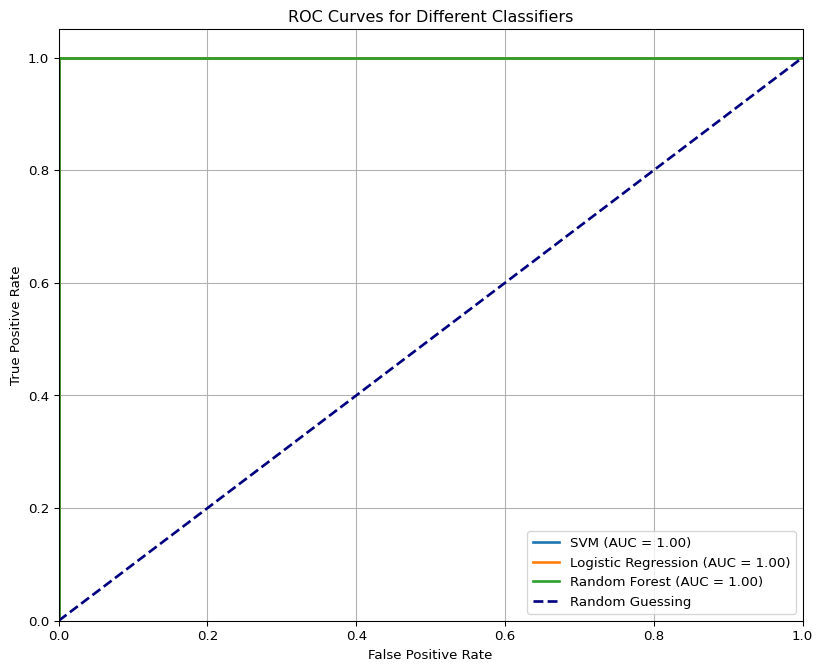
\includegraphics[keepaspectratio]{chapter6v2_files/figure-pdf/cell-8-output-1.png}}

\subsubsection{ROC Curve Components}\label{roc-curve-components}

\begin{itemize}
\tightlist
\item
  \textbf{True Positive Rate (TPR)}: TP / (TP + FN) - y-axis

  \begin{itemize}
  \tightlist
  \item
    Also known as Recall or Sensitivity
  \item
    Measures the proportion of actual positives correctly identified
  \end{itemize}
\item
  \textbf{False Positive Rate (FPR)}: FP / (FP + TN) - x-axis

  \begin{itemize}
  \tightlist
  \item
    Also known as (1 - Specificity)
  \item
    Measures the proportion of actual negatives incorrectly classified
    as positive
  \end{itemize}
\item
  \textbf{Classification Threshold}: Each point on the curve represents
  a different threshold

  \begin{itemize}
  \tightlist
  \item
    Moving along the curve represents changing the threshold for
    classifying a sample as positive
  \item
    Lower thresholds yield higher TPR but also higher FPR (upper right)
  \item
    Higher thresholds yield lower TPR but also lower FPR (lower left)
  \end{itemize}
\end{itemize}

\subsubsection{AUC (Area Under the ROC
Curve)}\label{auc-area-under-the-roc-curve}

The AUC metric quantifies the overall performance of a classifier:

\begin{itemize}
\tightlist
\item
  \textbf{AUC = 1.0}: Perfect classification (100\% sensitivity, 100\%
  specificity)
\item
  \textbf{AUC = 0.5}: No better than random guessing (shown as diagonal
  line)
\item
  \textbf{AUC \textless{} 0.5}: Worse than random guessing (rare,
  usually indicates an error)
\end{itemize}

AUC has an important probabilistic interpretation: if you randomly
select a positive and a negative example, the AUC represents the
probability that the classifier will rank the positive example higher
than the negative one.

\subsubsection{Precision-Recall Curve}\label{precision-recall-curve}

The Precision-Recall curve plots Precision against Recall at various
thresholds: - Particularly useful for imbalanced datasets where ROC
curves may be overly optimistic - The higher the curve (toward the
upper-right corner), the better the model - The area under the PR curve
(AUPRC) is another useful aggregate measure

\subsubsection{When to Use ROC vs.~PR
Curves}\label{when-to-use-roc-vs.-pr-curves}

\begin{itemize}
\tightlist
\item
  \textbf{ROC Curves}: Better when working with balanced datasets or
  when both classes are equally important
\item
  \textbf{Precision-Recall Curves}: Better for imbalanced datasets or
  when the positive class is of particular interest
\end{itemize}

\subsection{Regression Metrics}\label{regression-metrics}

\begin{Shaded}
\begin{Highlighting}[]
\CommentTok{\# Regression metrics example}
\ImportTok{from}\NormalTok{ sklearn.datasets }\ImportTok{import}\NormalTok{ load\_diabetes}
\ImportTok{from}\NormalTok{ sklearn.svm }\ImportTok{import}\NormalTok{ SVR}
\ImportTok{from}\NormalTok{ sklearn.metrics }\ImportTok{import}\NormalTok{ mean\_absolute\_error, mean\_squared\_error, r2\_score}

\CommentTok{\# Load diabetes dataset}
\NormalTok{diabetes }\OperatorTok{=}\NormalTok{ load\_diabetes()}
\NormalTok{X, y }\OperatorTok{=}\NormalTok{ diabetes.data, diabetes.target}

\CommentTok{\# Split data}
\NormalTok{X\_train, X\_test, y\_train, y\_test }\OperatorTok{=}\NormalTok{ train\_test\_split(X, y, test\_size}\OperatorTok{=}\FloatTok{0.3}\NormalTok{, random\_state}\OperatorTok{=}\DecValTok{42}\NormalTok{)}

\CommentTok{\# Scale features}
\NormalTok{scaler }\OperatorTok{=}\NormalTok{ StandardScaler()}
\NormalTok{X\_train }\OperatorTok{=}\NormalTok{ scaler.fit\_transform(X\_train)}
\NormalTok{X\_test }\OperatorTok{=}\NormalTok{ scaler.transform(X\_test)}

\CommentTok{\# Train SVR model}
\NormalTok{svr }\OperatorTok{=}\NormalTok{ SVR(kernel}\OperatorTok{=}\StringTok{\textquotesingle{}rbf\textquotesingle{}}\NormalTok{, C}\OperatorTok{=}\DecValTok{10}\NormalTok{, gamma}\OperatorTok{=}\StringTok{\textquotesingle{}scale\textquotesingle{}}\NormalTok{)}
\NormalTok{svr.fit(X\_train, y\_train)}

\CommentTok{\# Make predictions}
\NormalTok{y\_pred }\OperatorTok{=}\NormalTok{ svr.predict(X\_test)}

\CommentTok{\# Calculate regression metrics}
\NormalTok{mae }\OperatorTok{=}\NormalTok{ mean\_absolute\_error(y\_test, y\_pred)}
\NormalTok{mse }\OperatorTok{=}\NormalTok{ mean\_squared\_error(y\_test, y\_pred)}
\NormalTok{rmse }\OperatorTok{=}\NormalTok{ np.sqrt(mse)}
\NormalTok{r2 }\OperatorTok{=}\NormalTok{ r2\_score(y\_test, y\_pred)}

\BuiltInTok{print}\NormalTok{(}\SpecialStringTok{f"Mean Absolute Error (MAE): }\SpecialCharTok{\{}\NormalTok{mae}\SpecialCharTok{:.2f\}}\SpecialStringTok{"}\NormalTok{)}
\BuiltInTok{print}\NormalTok{(}\SpecialStringTok{f"Mean Squared Error (MSE): }\SpecialCharTok{\{}\NormalTok{mse}\SpecialCharTok{:.2f\}}\SpecialStringTok{"}\NormalTok{)}
\BuiltInTok{print}\NormalTok{(}\SpecialStringTok{f"Root Mean Squared Error (RMSE): }\SpecialCharTok{\{}\NormalTok{rmse}\SpecialCharTok{:.2f\}}\SpecialStringTok{"}\NormalTok{)}
\BuiltInTok{print}\NormalTok{(}\SpecialStringTok{f"R{-}squared (R²): }\SpecialCharTok{\{}\NormalTok{r2}\SpecialCharTok{:.2f\}}\SpecialStringTok{"}\NormalTok{)}

\CommentTok{\# Visualize actual vs predicted values}
\NormalTok{plt.figure(figsize}\OperatorTok{=}\NormalTok{(}\DecValTok{10}\NormalTok{, }\DecValTok{6}\NormalTok{))}
\NormalTok{plt.scatter(y\_test, y\_pred, alpha}\OperatorTok{=}\FloatTok{0.7}\NormalTok{)}
\NormalTok{plt.plot([y\_test.}\BuiltInTok{min}\NormalTok{(), y\_test.}\BuiltInTok{max}\NormalTok{()], [y\_test.}\BuiltInTok{min}\NormalTok{(), y\_test.}\BuiltInTok{max}\NormalTok{()], }\StringTok{\textquotesingle{}r{-}{-}\textquotesingle{}}\NormalTok{, lw}\OperatorTok{=}\DecValTok{2}\NormalTok{)}
\NormalTok{plt.xlabel(}\StringTok{\textquotesingle{}Actual Values\textquotesingle{}}\NormalTok{)}
\NormalTok{plt.ylabel(}\StringTok{\textquotesingle{}Predicted Values\textquotesingle{}}\NormalTok{)}
\NormalTok{plt.title(}\StringTok{\textquotesingle{}Actual vs Predicted Values (SVR)\textquotesingle{}}\NormalTok{)}
\NormalTok{plt.grid(}\VariableTok{True}\NormalTok{)}
\NormalTok{plt.show()}

\CommentTok{\# Plot residuals}
\NormalTok{residuals }\OperatorTok{=}\NormalTok{ y\_test }\OperatorTok{{-}}\NormalTok{ y\_pred}
\NormalTok{plt.figure(figsize}\OperatorTok{=}\NormalTok{(}\DecValTok{10}\NormalTok{, }\DecValTok{6}\NormalTok{))}
\NormalTok{plt.scatter(y\_pred, residuals, alpha}\OperatorTok{=}\FloatTok{0.7}\NormalTok{)}
\NormalTok{plt.axhline(y}\OperatorTok{=}\DecValTok{0}\NormalTok{, color}\OperatorTok{=}\StringTok{\textquotesingle{}r\textquotesingle{}}\NormalTok{, linestyle}\OperatorTok{=}\StringTok{\textquotesingle{}{-}{-}\textquotesingle{}}\NormalTok{, lw}\OperatorTok{=}\DecValTok{2}\NormalTok{)}
\NormalTok{plt.xlabel(}\StringTok{\textquotesingle{}Predicted Values\textquotesingle{}}\NormalTok{)}
\NormalTok{plt.ylabel(}\StringTok{\textquotesingle{}Residuals\textquotesingle{}}\NormalTok{)}
\NormalTok{plt.title(}\StringTok{\textquotesingle{}Residual Plot\textquotesingle{}}\NormalTok{)}
\NormalTok{plt.grid(}\VariableTok{True}\NormalTok{)}
\NormalTok{plt.show()}
\end{Highlighting}
\end{Shaded}

\begin{verbatim}
Mean Absolute Error (MAE): 41.38
Mean Squared Error (MSE): 2703.38
Root Mean Squared Error (RMSE): 51.99
R-squared (R²): 0.50
\end{verbatim}

\pandocbounded{\includegraphics[keepaspectratio]{chapter6v2_files/figure-pdf/cell-9-output-2.png}}

\pandocbounded{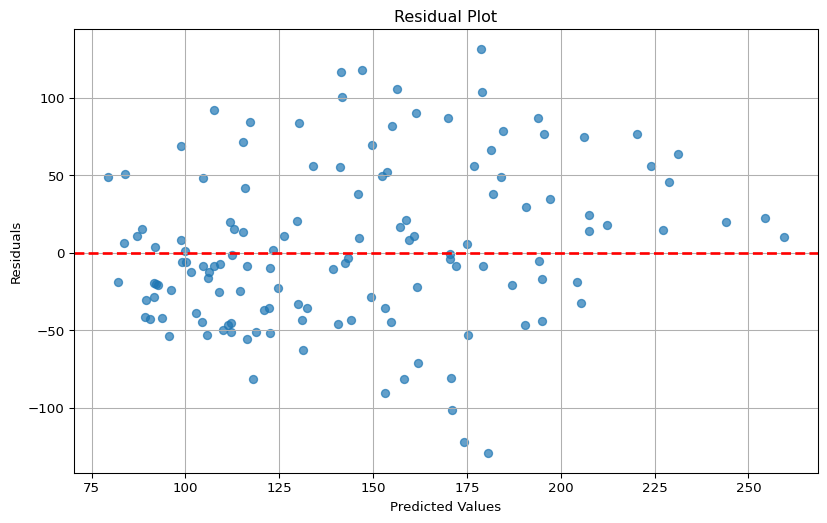
\includegraphics[keepaspectratio]{chapter6v2_files/figure-pdf/cell-9-output-3.png}}

\subsubsection{1. Mean Absolute Error
(MAE)}\label{mean-absolute-error-mae}

Average absolute difference between predictions and actual values: -
Formula: MAE = (1/n) × Σ\textbar yi - ŷi\textbar{} - Units match the
target variable - Robust to outliers since it doesn't square the errors
- All errors are weighted equally regardless of magnitude

\subsubsection{2. Mean Squared Error
(MSE)}\label{mean-squared-error-mse}

Average squared difference between predictions and actual values: -
Formula: MSE = (1/n) × Σ(yi - ŷi)² - Penalizes larger errors more due to
squaring - More sensitive to outliers than MAE - Units are squared (not
directly interpretable in terms of the original target)

\subsubsection{3. Root Mean Squared Error
(RMSE)}\label{root-mean-squared-error-rmse}

Square root of MSE, providing error in the same units as the target
variable: - Formula: RMSE = √MSE - More interpretable than MSE - Still
penalizes large errors more than small ones - Often used as the primary
metric for regression models

\subsubsection{4. R-Squared (R²)}\label{r-squared-ruxb2}

Proportion of variance explained by the model: - Formula: R² = 1 - (Σ(yi
- ŷi)²) / (Σ(yi - ȳ)²) - Range: 0 to 1 (higher is better) - R² = 0 means
the model is no better than predicting the mean - R² = 1 means perfect
prediction - Can be negative if model performs worse than just
predicting the mean - Scale-free, allowing comparison across different
target scales

\subsubsection{5. Adjusted R-Squared}\label{adjusted-r-squared}

Modified version of R² that adjusts for the number of predictors: -
Formula: Adjusted R² = 1 - {[}(1 - R²)(n - 1)/(n - p - 1){]} - Helps
prevent overfitting by penalizing excessive features - Increases only if
new features improve the model more than would be expected by chance

\subsection{Understanding Residual
Plots}\label{understanding-residual-plots}

Residual plots (predicted values vs.~residuals) help diagnose model
performance:

\begin{itemize}
\tightlist
\item
  \textbf{Random scatter around zero}: Indicates a good fit
\item
  \textbf{Funnel shape}: Indicates heteroscedasticity (non-constant
  variance)
\item
  \textbf{Curved pattern}: Suggests non-linear relationships weren't
  captured
\item
  \textbf{Clusters}: May indicate model misspecification or segmented
  data
\end{itemize}

\section{Model Fit Issues}\label{model-fit-issues}

\subsection{Underfitting
vs.~Overfitting}\label{underfitting-vs.-overfitting}

\bookmarksetup{startatroot}

\chapter{Demonstrate underfitting vs.~overfitting with polynomial
regression}\label{demonstrate-underfitting-vs.-overfitting-with-polynomial-regression}

from sklearn.preprocessing import PolynomialFeatures from
sklearn.linear\_model import LinearRegression from sklearn.pipeline
import Pipeline

\bookmarksetup{startatroot}

\chapter{Generate synthetic data}\label{generate-synthetic-data}

np.random.seed(42) X = np.sort(5 * np.random.rand(80, 1), axis=0) y =
np.sin(X).ravel() + 0.1 * np.random.randn(80)

\bookmarksetup{startatroot}

\chapter{Split into train and test}\label{split-into-train-and-test}

X\_train, X\_test, y\_train, y\_test = train\_test\_split(X, y,
test\_size=0.3, random\_state=42)

\bookmarksetup{startatroot}

\chapter{Create polynomials of different
degrees}\label{create-polynomials-of-different-degrees}

degrees = {[}1, 3, 15{]} \# Underfitting, good fit, overfitting
plt.figure(figsize=(16, 5))

for i, degree in enumerate(degrees): \# Create pipeline with polynomial
features and linear regression model = Pipeline({[} (`poly',
PolynomialFeatures(degree=degree)), (`linear', LinearRegression()) {]})

\begin{verbatim}
# Fit model
model.fit(X_train, y_train)

# Get predictions
y_train_pred = model.predict(X_train)
y_test_pred = model.predict(X_test)

# Calculate scores
train_r2 = r2_score(y_train, y_train_pred)
test_r2 = r2_score(y_test, y_test_pred)

# Plot results
plt.subplot(1, 3, i+1)

# Sort for smooth curve plotting
X_plot = np.linspace(0, 5, 100).reshape(-1, 1)
y_plot = model.predict(X_plot)

# Plot data and model
plt.scatter(X_train, y_train, color='blue', s=30, alpha=0.4, label='Training data')
plt.scatter(X_test, y_test, color='red', s=30, alpha=0.4, label='Testing data')
plt.plot(X_plot, y_plot, color='green', label=f'Degree {degree} polynomial')

plt.title(f'Polynomial Degree {degree}\nTrain R²: {train_r2:.2f}, Test R²: {test_r2:.2f}')
\end{verbatim}

\bookmarksetup{startatroot}

\chapter{Outlier Detection and Recommendation
Systems}\label{outlier-detection-and-recommendation-systems}

Outlier detection is a fundamental aspect of data analysis, helping to
identify data points that significantly deviate from the overall
pattern. These anomalies can indicate errors, rare events, or
interesting insights that merit further investigation.

\begin{tcolorbox}[enhanced jigsaw, coltitle=black, bottomrule=.15mm, breakable, opacityback=0, colback=white, bottomtitle=1mm, colbacktitle=quarto-callout-note-color!10!white, arc=.35mm, toptitle=1mm, titlerule=0mm, leftrule=.75mm, opacitybacktitle=0.6, colframe=quarto-callout-note-color-frame, left=2mm, title=\textcolor{quarto-callout-note-color}{\faInfo}\hspace{0.5em}{Why Outlier Detection Matters}, toprule=.15mm, rightrule=.15mm]

Outliers can significantly impact statistical analyses, model
performance, and business decisions. Detecting them is crucial for:

\begin{itemize}
\tightlist
\item
  Data cleaning and preprocessing
\item
  Fraud detection
\item
  Network intrusion detection
\item
  Medical diagnosis (detecting abnormal test results)
\item
  Manufacturing quality control
\end{itemize}

\end{tcolorbox}

\section{Graphical Outlier Detection}\label{graphical-outlier-detection}

One of the simplest ways to detect outliers is through visualization. By
plotting the data, human intuition can be leveraged to identify unusual
points. Common graphical methods include:

\begin{itemize}
\tightlist
\item
  \textbf{Boxplots}: Provide a summary of the data distribution,
  highlighting potential outliers
\item
  \textbf{Scatterplots}: Useful for detecting complex patterns in
  two-variable datasets
\item
  \textbf{Histograms}: Help identify values that fall outside the
  typical distribution
\end{itemize}

\begin{Shaded}
\begin{Highlighting}[]
\ImportTok{import}\NormalTok{ numpy }\ImportTok{as}\NormalTok{ np}
\ImportTok{import}\NormalTok{ matplotlib.pyplot }\ImportTok{as}\NormalTok{ plt}
\ImportTok{import}\NormalTok{ seaborn }\ImportTok{as}\NormalTok{ sns}
\ImportTok{import}\NormalTok{ pandas }\ImportTok{as}\NormalTok{ pd}

\CommentTok{\# Generate sample data with outliers}
\NormalTok{np.random.seed(}\DecValTok{42}\NormalTok{)}
\NormalTok{data }\OperatorTok{=}\NormalTok{ np.random.normal(}\DecValTok{0}\NormalTok{, }\DecValTok{1}\NormalTok{, }\DecValTok{100}\NormalTok{)}
\NormalTok{data }\OperatorTok{=}\NormalTok{ np.append(data, [}\DecValTok{5}\NormalTok{, }\OperatorTok{{-}}\DecValTok{5}\NormalTok{, }\DecValTok{7}\NormalTok{])  }\CommentTok{\# Add outliers}

\CommentTok{\# Create a box plot}
\NormalTok{plt.figure(figsize}\OperatorTok{=}\NormalTok{(}\DecValTok{10}\NormalTok{, }\DecValTok{6}\NormalTok{))}
\NormalTok{sns.boxplot(x}\OperatorTok{=}\NormalTok{data)}
\NormalTok{plt.title(}\StringTok{\textquotesingle{}Box Plot Showing Outliers\textquotesingle{}}\NormalTok{)}
\NormalTok{plt.tight\_layout()}
\NormalTok{plt.show()}

\CommentTok{\# Create a scatter plot}
\NormalTok{plt.figure(figsize}\OperatorTok{=}\NormalTok{(}\DecValTok{10}\NormalTok{, }\DecValTok{6}\NormalTok{))}
\NormalTok{plt.scatter(}\BuiltInTok{range}\NormalTok{(}\BuiltInTok{len}\NormalTok{(data)), data)}
\NormalTok{plt.title(}\StringTok{\textquotesingle{}Scatter Plot Showing Outliers\textquotesingle{}}\NormalTok{)}
\NormalTok{plt.ylabel(}\StringTok{\textquotesingle{}Value\textquotesingle{}}\NormalTok{)}
\NormalTok{plt.axhline(y}\OperatorTok{=}\NormalTok{np.mean(data) }\OperatorTok{+} \DecValTok{2}\OperatorTok{*}\NormalTok{np.std(data), color}\OperatorTok{=}\StringTok{\textquotesingle{}r\textquotesingle{}}\NormalTok{, linestyle}\OperatorTok{=}\StringTok{\textquotesingle{}{-}{-}\textquotesingle{}}\NormalTok{, label}\OperatorTok{=}\StringTok{\textquotesingle{}2σ Threshold\textquotesingle{}}\NormalTok{)}
\NormalTok{plt.axhline(y}\OperatorTok{=}\NormalTok{np.mean(data) }\OperatorTok{{-}} \DecValTok{2}\OperatorTok{*}\NormalTok{np.std(data), color}\OperatorTok{=}\StringTok{\textquotesingle{}r\textquotesingle{}}\NormalTok{, linestyle}\OperatorTok{=}\StringTok{\textquotesingle{}{-}{-}\textquotesingle{}}\NormalTok{)}
\NormalTok{plt.legend()}
\NormalTok{plt.tight\_layout()}
\NormalTok{plt.show()}
\end{Highlighting}
\end{Shaded}

\pandocbounded{\includegraphics[keepaspectratio]{chapter7_files/figure-pdf/cell-2-output-1.png}}

\pandocbounded{\includegraphics[keepaspectratio]{chapter7_files/figure-pdf/cell-2-output-2.png}}

\subsection{Quartiles and the Boxplot
Method}\label{quartiles-and-the-boxplot-method}

A boxplot divides data into quartiles, summarizing five key statistics:

\begin{itemize}
\tightlist
\item
  \textbf{Minimum}: The smallest value excluding outliers
\item
  \textbf{First quartile (Q1)}: The median of the lower half (25\% of
  data below Q1)
\item
  \textbf{Median}: The middle value of the dataset
\item
  \textbf{Third quartile (Q3)}: The median of the upper half (75\% of
  data below Q3)
\item
  \textbf{Maximum}: The largest value excluding outliers
\end{itemize}

A common rule for identifying outliers in boxplots is the 1.5 IQR rule:

\begin{itemize}
\tightlist
\item
  IQR (Interquartile Range) = Q3 - Q1
\item
  Any value above Q3 + 1.5 × IQR or below Q1 - 1.5 × IQR is considered
  an outlier.
\end{itemize}

This method is robust to extreme values and doesn't assume a specific
distribution, making it widely applicable.

\begin{Shaded}
\begin{Highlighting}[]
\CommentTok{\# Find outliers using the IQR method}
\KeywordTok{def}\NormalTok{ find\_outliers\_iqr(data):}
\NormalTok{    q1 }\OperatorTok{=}\NormalTok{ np.percentile(data, }\DecValTok{25}\NormalTok{)}
\NormalTok{    q3 }\OperatorTok{=}\NormalTok{ np.percentile(data, }\DecValTok{75}\NormalTok{)}
\NormalTok{    iqr }\OperatorTok{=}\NormalTok{ q3 }\OperatorTok{{-}}\NormalTok{ q1}
\NormalTok{    lower\_bound }\OperatorTok{=}\NormalTok{ q1 }\OperatorTok{{-}} \FloatTok{1.5} \OperatorTok{*}\NormalTok{ iqr}
\NormalTok{    upper\_bound }\OperatorTok{=}\NormalTok{ q3 }\OperatorTok{+} \FloatTok{1.5} \OperatorTok{*}\NormalTok{ iqr}
    
\NormalTok{    outliers }\OperatorTok{=}\NormalTok{ [x }\ControlFlowTok{for}\NormalTok{ x }\KeywordTok{in}\NormalTok{ data }\ControlFlowTok{if}\NormalTok{ x }\OperatorTok{\textless{}}\NormalTok{ lower\_bound }\KeywordTok{or}\NormalTok{ x }\OperatorTok{\textgreater{}}\NormalTok{ upper\_bound]}
\NormalTok{    outlier\_indices }\OperatorTok{=}\NormalTok{ [i }\ControlFlowTok{for}\NormalTok{ i, x }\KeywordTok{in} \BuiltInTok{enumerate}\NormalTok{(data) }\ControlFlowTok{if}\NormalTok{ x }\OperatorTok{\textless{}}\NormalTok{ lower\_bound }\KeywordTok{or}\NormalTok{ x }\OperatorTok{\textgreater{}}\NormalTok{ upper\_bound]}
    
    \ControlFlowTok{return}\NormalTok{ outliers, outlier\_indices, (lower\_bound, upper\_bound)}

\NormalTok{outliers, outlier\_indices, bounds }\OperatorTok{=}\NormalTok{ find\_outliers\_iqr(data)}
\BuiltInTok{print}\NormalTok{(}\SpecialStringTok{f"Outliers: }\SpecialCharTok{\{}\NormalTok{outliers}\SpecialCharTok{\}}\SpecialStringTok{"}\NormalTok{)}
\BuiltInTok{print}\NormalTok{(}\SpecialStringTok{f"Outlier indices: }\SpecialCharTok{\{}\NormalTok{outlier\_indices}\SpecialCharTok{\}}\SpecialStringTok{"}\NormalTok{)}
\BuiltInTok{print}\NormalTok{(}\SpecialStringTok{f"Bounds (lower, upper): }\SpecialCharTok{\{}\NormalTok{bounds}\SpecialCharTok{\}}\SpecialStringTok{"}\NormalTok{)}
\end{Highlighting}
\end{Shaded}

\begin{verbatim}
Outliers: [np.float64(-2.6197451040897444), np.float64(5.0), np.float64(-5.0), np.float64(7.0)]
Outlier indices: [74, 100, 101, 102]
Bounds (lower, upper): (np.float64(-2.260417817278694), np.float64(2.164235959266887))
\end{verbatim}

\section{Cluster-Based Outlier
Detection}\label{cluster-based-outlier-detection}

This method involves clustering data points and identifying those that
do not belong to any cluster or form small, isolated clusters. The
fundamental assumption is that normal data points belong to large, dense
clusters, while outliers either:

\begin{enumerate}
\def\labelenumi{\arabic{enumi}.}
\tightlist
\item
  Form small clusters far from the main clusters
\item
  Do not belong to any cluster
\item
  Are assigned to a cluster but are far from the cluster center
\end{enumerate}

Common clustering algorithms used for outlier detection include:

\begin{itemize}
\tightlist
\item
  \textbf{K-means Clustering}: Outliers are points that are far from any
  cluster mean or belong to a small cluster
\item
  \textbf{Density-Based Clustering} (e.g., DBSCAN): Outliers are data
  points that remain unassigned to clusters
\item
  \textbf{Hierarchical Clustering}: Outliers take longer to merge with
  other groups, making them distinguishable
\end{itemize}

\begin{Shaded}
\begin{Highlighting}[]
\ImportTok{from}\NormalTok{ sklearn.cluster }\ImportTok{import}\NormalTok{ KMeans}
\ImportTok{from}\NormalTok{ sklearn.datasets }\ImportTok{import}\NormalTok{ make\_blobs}

\CommentTok{\# Generate sample data with clusters and outliers}
\NormalTok{X, \_ }\OperatorTok{=}\NormalTok{ make\_blobs(n\_samples}\OperatorTok{=}\DecValTok{300}\NormalTok{, centers}\OperatorTok{=}\DecValTok{3}\NormalTok{, cluster\_std}\OperatorTok{=}\FloatTok{0.60}\NormalTok{, random\_state}\OperatorTok{=}\DecValTok{0}\NormalTok{)}
\CommentTok{\# Add some outliers}
\NormalTok{X }\OperatorTok{=}\NormalTok{ np.vstack([X, np.array([[}\DecValTok{6}\NormalTok{, }\DecValTok{6}\NormalTok{], [}\OperatorTok{{-}}\DecValTok{6}\NormalTok{, }\OperatorTok{{-}}\DecValTok{6}\NormalTok{], [}\DecValTok{6}\NormalTok{, }\OperatorTok{{-}}\DecValTok{6}\NormalTok{], [}\OperatorTok{{-}}\DecValTok{6}\NormalTok{, }\DecValTok{6}\NormalTok{]])])}

\CommentTok{\# Apply K{-}means clustering}
\NormalTok{kmeans }\OperatorTok{=}\NormalTok{ KMeans(n\_clusters}\OperatorTok{=}\DecValTok{3}\NormalTok{, random\_state}\OperatorTok{=}\DecValTok{0}\NormalTok{)}
\NormalTok{cluster\_labels }\OperatorTok{=}\NormalTok{ kmeans.fit\_predict(X)}
\NormalTok{cluster\_centers }\OperatorTok{=}\NormalTok{ kmeans.cluster\_centers\_}

\CommentTok{\# Calculate distance of each point to its cluster center}
\NormalTok{distances }\OperatorTok{=}\NormalTok{ np.zeros(X.shape[}\DecValTok{0}\NormalTok{])}
\ControlFlowTok{for}\NormalTok{ i }\KeywordTok{in} \BuiltInTok{range}\NormalTok{(X.shape[}\DecValTok{0}\NormalTok{]):}
\NormalTok{    cluster\_idx }\OperatorTok{=}\NormalTok{ cluster\_labels[i]}
\NormalTok{    distances[i] }\OperatorTok{=}\NormalTok{ np.linalg.norm(X[i] }\OperatorTok{{-}}\NormalTok{ cluster\_centers[cluster\_idx])}

\CommentTok{\# Identify potential outliers (points with largest distances)}
\NormalTok{threshold }\OperatorTok{=}\NormalTok{ np.percentile(distances, }\DecValTok{95}\NormalTok{)  }\CommentTok{\# Top 5\% as outliers}
\NormalTok{outlier\_mask }\OperatorTok{=}\NormalTok{ distances }\OperatorTok{\textgreater{}}\NormalTok{ threshold}

\CommentTok{\# Visualize the clusters and outliers}
\NormalTok{plt.figure(figsize}\OperatorTok{=}\NormalTok{(}\DecValTok{10}\NormalTok{, }\DecValTok{8}\NormalTok{))}
\NormalTok{plt.scatter(X[}\OperatorTok{\textasciitilde{}}\NormalTok{outlier\_mask, }\DecValTok{0}\NormalTok{], X[}\OperatorTok{\textasciitilde{}}\NormalTok{outlier\_mask, }\DecValTok{1}\NormalTok{], c}\OperatorTok{=}\NormalTok{cluster\_labels[}\OperatorTok{\textasciitilde{}}\NormalTok{outlier\_mask], }
\NormalTok{            cmap}\OperatorTok{=}\StringTok{\textquotesingle{}viridis\textquotesingle{}}\NormalTok{, marker}\OperatorTok{=}\StringTok{\textquotesingle{}o\textquotesingle{}}\NormalTok{, s}\OperatorTok{=}\DecValTok{50}\NormalTok{, alpha}\OperatorTok{=}\FloatTok{0.8}\NormalTok{)}
\NormalTok{plt.scatter(X[outlier\_mask, }\DecValTok{0}\NormalTok{], X[outlier\_mask, }\DecValTok{1}\NormalTok{], c}\OperatorTok{=}\StringTok{\textquotesingle{}red\textquotesingle{}}\NormalTok{, marker}\OperatorTok{=}\StringTok{\textquotesingle{}x\textquotesingle{}}\NormalTok{, s}\OperatorTok{=}\DecValTok{100}\NormalTok{, label}\OperatorTok{=}\StringTok{\textquotesingle{}Outliers\textquotesingle{}}\NormalTok{)}
\NormalTok{plt.scatter(cluster\_centers[:, }\DecValTok{0}\NormalTok{], cluster\_centers[:, }\DecValTok{1}\NormalTok{], c}\OperatorTok{=}\StringTok{\textquotesingle{}black\textquotesingle{}}\NormalTok{, marker}\OperatorTok{=}\StringTok{\textquotesingle{}*\textquotesingle{}}\NormalTok{, s}\OperatorTok{=}\DecValTok{200}\NormalTok{, label}\OperatorTok{=}\StringTok{\textquotesingle{}Centroids\textquotesingle{}}\NormalTok{)}
\NormalTok{plt.legend()}
\NormalTok{plt.title(}\StringTok{\textquotesingle{}K{-}means Clustering with Outlier Detection\textquotesingle{}}\NormalTok{)}
\NormalTok{plt.tight\_layout()}
\NormalTok{plt.show()}
\end{Highlighting}
\end{Shaded}

\pandocbounded{\includegraphics[keepaspectratio]{chapter7_files/figure-pdf/cell-4-output-1.png}}

\section{Distance-Based Outlier
Detection}\label{distance-based-outlier-detection}

Rather than relying on visualization or clustering, distance-based
methods use spatial relationships to detect anomalies. These approaches
are particularly useful for high-dimensional data where visualization
becomes challenging.

\subsection{Global Distance-Based Detection
(KNN)}\label{global-distance-based-detection-knn}

The K-Nearest Neighbors (KNN) approach for outlier detection follows
these steps:

\begin{enumerate}
\def\labelenumi{\arabic{enumi}.}
\tightlist
\item
  Compute the average distance of each point to its K-nearest neighbors
\item
  Sort these distances and flag the largest ones as outliers
\item
  This is useful for identifying global outliers that deviate from the
  overall data distribution
\end{enumerate}

\subsection{Local Distance-Based
Detection}\label{local-distance-based-detection}

Local distance-based methods account for varying data densities by
considering the locality of each point:

\begin{enumerate}
\def\labelenumi{\arabic{enumi}.}
\tightlist
\item
  An outlier's `outlierness' is determined by comparing its distance to
  neighbors relative to how far those neighbors are from their own
  neighbors
\item
  If the ratio exceeds 1, the point is flagged as an outlier
\item
  This approach can detect local outliers in datasets with varying
  densities
\end{enumerate}

\begin{Shaded}
\begin{Highlighting}[]
\ImportTok{from}\NormalTok{ sklearn.neighbors }\ImportTok{import}\NormalTok{ NearestNeighbors}

\CommentTok{\# Generate sample 2D data}
\NormalTok{np.random.seed(}\DecValTok{42}\NormalTok{)}
\NormalTok{X\_normal }\OperatorTok{=}\NormalTok{ np.random.normal(}\DecValTok{0}\NormalTok{, }\DecValTok{1}\NormalTok{, (}\DecValTok{100}\NormalTok{, }\DecValTok{2}\NormalTok{))}
\NormalTok{X\_outliers }\OperatorTok{=}\NormalTok{ np.random.uniform(}\OperatorTok{{-}}\DecValTok{4}\NormalTok{, }\DecValTok{4}\NormalTok{, (}\DecValTok{5}\NormalTok{, }\DecValTok{2}\NormalTok{))}
\NormalTok{X }\OperatorTok{=}\NormalTok{ np.vstack([X\_normal, X\_outliers])}

\CommentTok{\# Find k{-}nearest neighbors}
\NormalTok{k }\OperatorTok{=} \DecValTok{5}
\NormalTok{nbrs }\OperatorTok{=}\NormalTok{ NearestNeighbors(n\_neighbors}\OperatorTok{=}\NormalTok{k).fit(X)}
\NormalTok{distances, indices }\OperatorTok{=}\NormalTok{ nbrs.kneighbors(X)}

\CommentTok{\# Calculate average distance to k{-}nearest neighbors}
\NormalTok{avg\_knn\_distance }\OperatorTok{=}\NormalTok{ distances[:, }\DecValTok{1}\NormalTok{:].mean(axis}\OperatorTok{=}\DecValTok{1}\NormalTok{)  }\CommentTok{\# Exclude self (distance=0)}

\CommentTok{\# Identify outliers}
\NormalTok{threshold }\OperatorTok{=}\NormalTok{ np.percentile(avg\_knn\_distance, }\DecValTok{95}\NormalTok{)}
\NormalTok{outlier\_mask }\OperatorTok{=}\NormalTok{ avg\_knn\_distance }\OperatorTok{\textgreater{}}\NormalTok{ threshold}

\CommentTok{\# Visualize results}
\NormalTok{plt.figure(figsize}\OperatorTok{=}\NormalTok{(}\DecValTok{10}\NormalTok{, }\DecValTok{8}\NormalTok{))}
\NormalTok{plt.scatter(X[}\OperatorTok{\textasciitilde{}}\NormalTok{outlier\_mask, }\DecValTok{0}\NormalTok{], X[}\OperatorTok{\textasciitilde{}}\NormalTok{outlier\_mask, }\DecValTok{1}\NormalTok{], c}\OperatorTok{=}\StringTok{\textquotesingle{}blue\textquotesingle{}}\NormalTok{, label}\OperatorTok{=}\StringTok{\textquotesingle{}Normal points\textquotesingle{}}\NormalTok{)}
\NormalTok{plt.scatter(X[outlier\_mask, }\DecValTok{0}\NormalTok{], X[outlier\_mask, }\DecValTok{1}\NormalTok{], c}\OperatorTok{=}\StringTok{\textquotesingle{}red\textquotesingle{}}\NormalTok{, marker}\OperatorTok{=}\StringTok{\textquotesingle{}x\textquotesingle{}}\NormalTok{, s}\OperatorTok{=}\DecValTok{100}\NormalTok{, label}\OperatorTok{=}\StringTok{\textquotesingle{}Outliers\textquotesingle{}}\NormalTok{)}
\NormalTok{plt.title(}\SpecialStringTok{f\textquotesingle{}KNN Distance{-}Based Outlier Detection (k=}\SpecialCharTok{\{}\NormalTok{k}\SpecialCharTok{\}}\SpecialStringTok{)\textquotesingle{}}\NormalTok{)}
\NormalTok{plt.legend()}
\NormalTok{plt.tight\_layout()}
\NormalTok{plt.show()}
\end{Highlighting}
\end{Shaded}

\pandocbounded{\includegraphics[keepaspectratio]{chapter7_files/figure-pdf/cell-5-output-1.png}}

\section{Tree-Based Outlier Detection: Isolation
Forests}\label{tree-based-outlier-detection-isolation-forests}

Isolation Forests provide a tree-based approach to anomaly detection,
making them highly efficient for large and high-dimensional datasets.
This method partitions data randomly to isolate anomalies based on the
principle that outliers are ``few and different'' and therefore should
be easier to isolate.

\textbf{Key Features:}

\begin{itemize}
\tightlist
\item
  Uses multiple decision trees to calculate anomaly scores
\item
  Has linear time complexity, making it scalable for large datasets
\item
  Does not require assumptions about feature distributions
\item
  Works best with large datasets but performs poorly on small datasets
\item
  Can detect anomalies without prior knowledge but does not explain why
  a point is anomalous
\end{itemize}

\textbf{Steps of Isolation Forest Algorithm:}

\begin{enumerate}
\def\labelenumi{\arabic{enumi}.}
\tightlist
\item
  Randomly select a feature
\item
  Randomly choose a split value within the feature's range
\item
  Partition the data into two child nodes
\item
  Recursively repeat the process until:

  \begin{itemize}
  \tightlist
  \item
    Each leaf node has only one instance
  \item
    A predefined maximum depth is reached
  \end{itemize}
\end{enumerate}

The anomaly score is calculated based on the path length to isolate a
point. Outliers typically have shorter path lengths.

\begin{Shaded}
\begin{Highlighting}[]
\ImportTok{from}\NormalTok{ sklearn.ensemble }\ImportTok{import}\NormalTok{ IsolationForest}

\CommentTok{\# Generate sample data with outliers}
\NormalTok{np.random.seed(}\DecValTok{42}\NormalTok{)}
\NormalTok{X\_normal }\OperatorTok{=}\NormalTok{ np.random.normal(}\DecValTok{0}\NormalTok{, }\DecValTok{1}\NormalTok{, (}\DecValTok{100}\NormalTok{, }\DecValTok{2}\NormalTok{))}
\NormalTok{X\_outliers }\OperatorTok{=}\NormalTok{ np.random.uniform(}\OperatorTok{{-}}\DecValTok{4}\NormalTok{, }\DecValTok{4}\NormalTok{, (}\DecValTok{5}\NormalTok{, }\DecValTok{2}\NormalTok{))}
\NormalTok{X }\OperatorTok{=}\NormalTok{ np.vstack([X\_normal, X\_outliers])}

\CommentTok{\# Apply Isolation Forest}
\NormalTok{iso\_forest }\OperatorTok{=}\NormalTok{ IsolationForest(contamination}\OperatorTok{=}\FloatTok{0.05}\NormalTok{, random\_state}\OperatorTok{=}\DecValTok{42}\NormalTok{)}
\NormalTok{predictions }\OperatorTok{=}\NormalTok{ iso\_forest.fit\_predict(X)}
\NormalTok{outlier\_mask }\OperatorTok{=}\NormalTok{ predictions }\OperatorTok{==} \OperatorTok{{-}}\DecValTok{1}  \CommentTok{\# {-}1 for outliers, 1 for inliers}

\CommentTok{\# Visualize results}
\NormalTok{plt.figure(figsize}\OperatorTok{=}\NormalTok{(}\DecValTok{10}\NormalTok{, }\DecValTok{8}\NormalTok{))}
\NormalTok{plt.scatter(X[}\OperatorTok{\textasciitilde{}}\NormalTok{outlier\_mask, }\DecValTok{0}\NormalTok{], X[}\OperatorTok{\textasciitilde{}}\NormalTok{outlier\_mask, }\DecValTok{1}\NormalTok{], c}\OperatorTok{=}\StringTok{\textquotesingle{}blue\textquotesingle{}}\NormalTok{, label}\OperatorTok{=}\StringTok{\textquotesingle{}Normal points\textquotesingle{}}\NormalTok{)}
\NormalTok{plt.scatter(X[outlier\_mask, }\DecValTok{0}\NormalTok{], X[outlier\_mask, }\DecValTok{1}\NormalTok{], c}\OperatorTok{=}\StringTok{\textquotesingle{}red\textquotesingle{}}\NormalTok{, marker}\OperatorTok{=}\StringTok{\textquotesingle{}x\textquotesingle{}}\NormalTok{, s}\OperatorTok{=}\DecValTok{100}\NormalTok{, label}\OperatorTok{=}\StringTok{\textquotesingle{}Outliers\textquotesingle{}}\NormalTok{)}
\NormalTok{plt.title(}\StringTok{\textquotesingle{}Isolation Forest Outlier Detection\textquotesingle{}}\NormalTok{)}
\NormalTok{plt.legend()}
\NormalTok{plt.tight\_layout()}
\NormalTok{plt.show()}

\CommentTok{\# Show anomaly scores}
\NormalTok{anomaly\_scores }\OperatorTok{=}\NormalTok{ iso\_forest.decision\_function(X)}
\NormalTok{plt.figure(figsize}\OperatorTok{=}\NormalTok{(}\DecValTok{10}\NormalTok{, }\DecValTok{6}\NormalTok{))}
\NormalTok{plt.hist(anomaly\_scores, bins}\OperatorTok{=}\DecValTok{20}\NormalTok{)}
\NormalTok{plt.axvline(x}\OperatorTok{=}\DecValTok{0}\NormalTok{, color}\OperatorTok{=}\StringTok{\textquotesingle{}r\textquotesingle{}}\NormalTok{, linestyle}\OperatorTok{=}\StringTok{\textquotesingle{}{-}{-}\textquotesingle{}}\NormalTok{)}
\NormalTok{plt.title(}\StringTok{\textquotesingle{}Isolation Forest Anomaly Scores (lower = more anomalous)\textquotesingle{}}\NormalTok{)}
\NormalTok{plt.xlabel(}\StringTok{\textquotesingle{}Score\textquotesingle{}}\NormalTok{)}
\NormalTok{plt.ylabel(}\StringTok{\textquotesingle{}Count\textquotesingle{}}\NormalTok{)}
\NormalTok{plt.tight\_layout()}
\NormalTok{plt.show()}
\end{Highlighting}
\end{Shaded}

\pandocbounded{\includegraphics[keepaspectratio]{chapter7_files/figure-pdf/cell-6-output-1.png}}

\pandocbounded{\includegraphics[keepaspectratio]{chapter7_files/figure-pdf/cell-6-output-2.png}}

\section{Challenges in Unsupervised Outlier
Detection}\label{challenges-in-unsupervised-outlier-detection}

While unsupervised methods are powerful, they come with challenges:

\begin{itemize}
\tightlist
\item
  \textbf{False positives}: Legitimate data points may be flagged as
  outliers
\item
  \textbf{Domain-specific outliers}: What constitutes an outlier varies
  by domain
\item
  \textbf{Parameter sensitivity}: Results depend on parameter choices (k
  in KNN, contamination in Isolation Forest)
\item
  \textbf{Dismissal of true anomalies}: A notable example is the delayed
  discovery of the ozone hole, which remained undetected for years
  because the anomaly was disregarded by automated systems
\end{itemize}

Striking a balance between reporting genuine outliers and avoiding
excessive false positives is crucial in data-driven decision-making.

\bookmarksetup{startatroot}

\chapter{Recommender Systems}\label{recommender-systems}

Recommender systems play a crucial role in online retail, content
platforms, and various digital services by helping businesses suggest
relevant products to customers. By analyzing user behavior, purchase
history, and product similarities, recommendation algorithms improve
user experience and increase sales.

\begin{tcolorbox}[enhanced jigsaw, coltitle=black, bottomrule=.15mm, breakable, opacityback=0, colback=white, bottomtitle=1mm, colbacktitle=quarto-callout-tip-color!10!white, arc=.35mm, toptitle=1mm, titlerule=0mm, leftrule=.75mm, opacitybacktitle=0.6, colframe=quarto-callout-tip-color-frame, left=2mm, title=\textcolor{quarto-callout-tip-color}{\faLightbulb}\hspace{0.5em}{Business Impact of Recommender Systems}, toprule=.15mm, rightrule=.15mm]

\begin{itemize}
\tightlist
\item
  35\% of Amazon's revenue comes from recommendations
\item
  75\% of Netflix views are driven by recommendations
\item
  Spotify's Discover Weekly has a 55\% click-through rate
\end{itemize}

\end{tcolorbox}

\section{Recommendation Scenarios}\label{recommendation-scenarios}

Recommender systems operate in different contexts:

\begin{itemize}
\tightlist
\item
  \textbf{Item-based recommendation}: Suggest items similar to a given
  item (e.g., Amazon's ``Customers who bought this also bought'')
\item
  \textbf{User-based recommendation}: Suggest items to a user based on
  their past behavior (e.g., Netflix homepage)
\item
  \textbf{Hybrid recommendation}: Combines both item-based and
  user-based approaches for personalized recommendations
\end{itemize}

A key challenge is that users rate only a small fraction of available
items, leading to a sparse user-item matrix. The system must predict
missing ratings to provide effective recommendations.

\section{Types of Recommender
Systems}\label{types-of-recommender-systems}

\subsection{1. Content-Based Filtering}\label{content-based-filtering}

Content-based filtering recommends items similar to those a user has
liked in the past based on item features:

\begin{itemize}
\tightlist
\item
  \textbf{Assumptions}: Access to side information about items (e.g.,
  genre, keywords, descriptions)
\item
  \textbf{Approach}: Uses supervised learning to extract item and user
  features, then builds a model to predict ratings
\item
  \textbf{Advantages}: Can make recommendations for new users/items
  without requiring previous interactions
\item
  \textbf{Real-world examples}:

  \begin{itemize}
  \tightlist
  \item
    Pandora (music recommendations based on song attributes)
  \item
    Gmail's important messages (predicting which emails are important
    based on content)
  \end{itemize}
\end{itemize}

\subsection{2. Collaborative Filtering}\label{collaborative-filtering}

Collaborative filtering recommends items based on similarity patterns
between users and/or items:

\begin{itemize}
\tightlist
\item
  \textbf{Assumptions}: Does not require side information about items
\item
  \textbf{Core idea}: Personal tastes are correlated. If Alice and Bob
  both like X, and Alice likes Y, then Bob is more likely to like Y
\item
  \textbf{Approach}: Uses an unsupervised learning approach. Have labels
  (ratings) but no explicit feature vectors
\item
  \textbf{Limitations}: Struggles with the cold start problem (poor
  predictions for new users or items)
\end{itemize}

\section{User-Product Matrix}\label{user-product-matrix}

The user-product matrix represents users as rows and products as
columns, with entries indicating purchases or ratings. This matrix is
the foundation of many recommendation algorithms.

\begin{Shaded}
\begin{Highlighting}[]
\CommentTok{\# Create a sample user{-}item matrix}
\NormalTok{users }\OperatorTok{=}\NormalTok{ [}\StringTok{\textquotesingle{}User1\textquotesingle{}}\NormalTok{, }\StringTok{\textquotesingle{}User2\textquotesingle{}}\NormalTok{, }\StringTok{\textquotesingle{}User3\textquotesingle{}}\NormalTok{, }\StringTok{\textquotesingle{}User4\textquotesingle{}}\NormalTok{, }\StringTok{\textquotesingle{}User5\textquotesingle{}}\NormalTok{]}
\NormalTok{items }\OperatorTok{=}\NormalTok{ [}\StringTok{\textquotesingle{}Item1\textquotesingle{}}\NormalTok{, }\StringTok{\textquotesingle{}Item2\textquotesingle{}}\NormalTok{, }\StringTok{\textquotesingle{}Item3\textquotesingle{}}\NormalTok{, }\StringTok{\textquotesingle{}Item4\textquotesingle{}}\NormalTok{, }\StringTok{\textquotesingle{}Item5\textquotesingle{}}\NormalTok{]}
\NormalTok{np.random.seed(}\DecValTok{42}\NormalTok{)}
\NormalTok{ratings }\OperatorTok{=}\NormalTok{ np.zeros((}\BuiltInTok{len}\NormalTok{(users), }\BuiltInTok{len}\NormalTok{(items)))}
\CommentTok{\# Fill with some ratings (1{-}5), 0 means no rating}
\ControlFlowTok{for}\NormalTok{ i }\KeywordTok{in} \BuiltInTok{range}\NormalTok{(}\BuiltInTok{len}\NormalTok{(users)):}
    \ControlFlowTok{for}\NormalTok{ j }\KeywordTok{in} \BuiltInTok{range}\NormalTok{(}\BuiltInTok{len}\NormalTok{(items)):}
        \ControlFlowTok{if}\NormalTok{ np.random.random() }\OperatorTok{\textgreater{}} \FloatTok{0.3}\NormalTok{:  }\CommentTok{\# 70\% chance of having a rating}
\NormalTok{            ratings[i, j] }\OperatorTok{=}\NormalTok{ np.random.randint(}\DecValTok{1}\NormalTok{, }\DecValTok{6}\NormalTok{)}

\CommentTok{\# Create a DataFrame for better visualization}
\NormalTok{ratings\_df }\OperatorTok{=}\NormalTok{ pd.DataFrame(ratings, index}\OperatorTok{=}\NormalTok{users, columns}\OperatorTok{=}\NormalTok{items)}
\BuiltInTok{print}\NormalTok{(}\StringTok{"User{-}Item Rating Matrix:"}\NormalTok{)}
\BuiltInTok{print}\NormalTok{(ratings\_df)}

\CommentTok{\# Visualize the matrix}
\NormalTok{plt.figure(figsize}\OperatorTok{=}\NormalTok{(}\DecValTok{10}\NormalTok{, }\DecValTok{8}\NormalTok{))}
\NormalTok{sns.heatmap(ratings\_df, annot}\OperatorTok{=}\VariableTok{True}\NormalTok{, cmap}\OperatorTok{=}\StringTok{\textquotesingle{}YlGnBu\textquotesingle{}}\NormalTok{, cbar\_kws}\OperatorTok{=}\NormalTok{\{}\StringTok{\textquotesingle{}label\textquotesingle{}}\NormalTok{: }\StringTok{\textquotesingle{}Rating\textquotesingle{}}\NormalTok{\})}
\NormalTok{plt.title(}\StringTok{\textquotesingle{}User{-}Item Rating Matrix\textquotesingle{}}\NormalTok{)}
\NormalTok{plt.tight\_layout()}
\NormalTok{plt.show()}
\end{Highlighting}
\end{Shaded}

\begin{verbatim}
User-Item Rating Matrix:
       Item1  Item2  Item3  Item4  Item5
User1    5.0    0.0    5.0    0.0    0.0
User2    0.0    4.0    0.0    5.0    4.0
User3    2.0    0.0    0.0    5.0    1.0
User4    2.0    0.0    3.0    4.0    3.0
User5    5.0    2.0    4.0    2.0    5.0
\end{verbatim}

\pandocbounded{\includegraphics[keepaspectratio]{chapter7_files/figure-pdf/cell-7-output-2.png}}

\section{Collaborative Filtering
Methods}\label{collaborative-filtering-methods}

\subsection{1. Neighborhood Methods}\label{neighborhood-methods}

Neighborhood methods find users or items with similar preferences:

\begin{itemize}
\tightlist
\item
  \textbf{User-based}: If a group of users liked the same set of movies,
  recommend those movies to others in the group
\item
  \textbf{Item-based}: If two items have similar rating patterns,
  recommend one to users who liked the other
\end{itemize}

\textbf{Algorithm:} 1. Identify similar users/movies based on rating
patterns 2. Recommend movies watched by similar users

Amazon's Product Recommendation Method uses nearest neighbor (KNN)
searches across product columns to determine similarity. The goal is to
find products that minimize the difference between them:

\begin{itemize}
\tightlist
\item
  Normalize each column by dividing by its norm:
  \(\hat{X}_j = \frac{X_j}{\|X_j\|}\)
\item
  This ensures that recommendations reflect the relative popularity of a
  product rather than absolute purchase counts
\item
  Products bought by similar users are considered more alike
\end{itemize}

\begin{Shaded}
\begin{Highlighting}[]
\ImportTok{from}\NormalTok{ sklearn.metrics.pairwise }\ImportTok{import}\NormalTok{ cosine\_similarity}

\CommentTok{\# Compute item{-}item similarity matrix}
\NormalTok{item\_similarity }\OperatorTok{=}\NormalTok{ cosine\_similarity(ratings\_df.T)}
\NormalTok{item\_sim\_df }\OperatorTok{=}\NormalTok{ pd.DataFrame(item\_similarity, index}\OperatorTok{=}\NormalTok{items, columns}\OperatorTok{=}\NormalTok{items)}
\BuiltInTok{print}\NormalTok{(}\StringTok{"Item{-}Item Similarity Matrix:"}\NormalTok{)}
\BuiltInTok{print}\NormalTok{(item\_sim\_df)}

\CommentTok{\# Visualize item similarity}
\NormalTok{plt.figure(figsize}\OperatorTok{=}\NormalTok{(}\DecValTok{10}\NormalTok{, }\DecValTok{8}\NormalTok{))}
\NormalTok{sns.heatmap(item\_sim\_df, annot}\OperatorTok{=}\VariableTok{True}\NormalTok{, cmap}\OperatorTok{=}\StringTok{\textquotesingle{}coolwarm\textquotesingle{}}\NormalTok{, vmin}\OperatorTok{={-}}\DecValTok{1}\NormalTok{, vmax}\OperatorTok{=}\DecValTok{1}\NormalTok{)}
\NormalTok{plt.title(}\StringTok{\textquotesingle{}Item{-}Item Similarity Matrix (Cosine Similarity)\textquotesingle{}}\NormalTok{)}
\NormalTok{plt.tight\_layout()}
\NormalTok{plt.show()}

\CommentTok{\# Function to get top N similar items}
\KeywordTok{def}\NormalTok{ get\_similar\_items(item\_name, item\_sim\_df, n}\OperatorTok{=}\DecValTok{2}\NormalTok{):}
\NormalTok{    similar\_items }\OperatorTok{=}\NormalTok{ item\_sim\_df[item\_name].sort\_values(ascending}\OperatorTok{=}\VariableTok{False}\NormalTok{)}
    \CommentTok{\# Exclude the item itself}
\NormalTok{    similar\_items }\OperatorTok{=}\NormalTok{ similar\_items.drop(item\_name)}
    \ControlFlowTok{return}\NormalTok{ similar\_items.head(n)}

\CommentTok{\# Example: Get items similar to Item1}
\NormalTok{similar\_to\_item1 }\OperatorTok{=}\NormalTok{ get\_similar\_items(}\StringTok{\textquotesingle{}Item1\textquotesingle{}}\NormalTok{, item\_sim\_df)}
\BuiltInTok{print}\NormalTok{(}\StringTok{"}\CharTok{\textbackslash{}n}\StringTok{Items similar to Item1:"}\NormalTok{)}
\BuiltInTok{print}\NormalTok{(similar\_to\_item1)}
\end{Highlighting}
\end{Shaded}

\begin{verbatim}
Item-Item Similarity Matrix:
          Item1     Item2     Item3     Item4     Item5
Item1  1.000000  0.293610  0.947046  0.439435  0.606757
Item2  0.293610  1.000000  0.252982  0.641427  0.814092
Item3  0.947046  0.252982  1.000000  0.338062  0.574286
Item4  0.439435  0.641427  0.338062  1.000000  0.786618
Item5  0.606757  0.814092  0.574286  0.786618  1.000000
\end{verbatim}

\pandocbounded{\includegraphics[keepaspectratio]{chapter7_files/figure-pdf/cell-8-output-2.png}}

\begin{verbatim}

Items similar to Item1:
Item3    0.947046
Item5    0.606757
Name: Item1, dtype: float64
\end{verbatim}

\subsection{2. Latent Factor Methods}\label{latent-factor-methods}

Instead of looking at raw ratings, latent factor models assume that both
users and movies exist in a lower-dimensional feature space representing
hidden properties.

\begin{itemize}
\tightlist
\item
  Each movie and user is mapped to a vector in this space
\item
  Recommendations are made based on proximity in this latent space
\end{itemize}

\textbf{Example:} A user interested in action movies might have a high
latent factor score for ``intensity,'' leading to recommendations for
high-action films.

\section{Matrix Factorization (MF)}\label{matrix-factorization-mf}

Matrix Factorization is a powerful approach to collaborative filtering,
decomposing the user-item matrix into lower-dimensional factors:

\begin{itemize}
\tightlist
\item
  Defines a model with an objective function
\item
  Optimized using stochastic gradient descent
\end{itemize}

\textbf{Types of Matrix Factorization:} - Unconstrained Matrix
Factorization - Singular Value Decomposition (SVD) - Non-negative Matrix
Factorization (NMF)

\textbf{Mathematical Formulation:} For a user-item matrix \(R\) with
users \(u\) and items \(i\), matrix factorization finds matrices \(P\)
and \(Q\) such that:

\(R \approx P \times Q^T\)

Where \(P\) represents user vectors and \(Q\) represents item vectors in
the latent space.

\begin{Shaded}
\begin{Highlighting}[]
\ImportTok{from}\NormalTok{ sklearn.decomposition }\ImportTok{import}\NormalTok{ NMF}

\CommentTok{\# Fill missing values with zeros for demonstration}
\CommentTok{\# In practice, you might want to use mean imputation or more sophisticated methods}
\NormalTok{ratings\_matrix }\OperatorTok{=}\NormalTok{ ratings\_df.values}

\CommentTok{\# Non{-}negative Matrix Factorization}
\NormalTok{n\_components }\OperatorTok{=} \DecValTok{2}  \CommentTok{\# Number of latent factors}
\NormalTok{model }\OperatorTok{=}\NormalTok{ NMF(n\_components}\OperatorTok{=}\NormalTok{n\_components, init}\OperatorTok{=}\StringTok{\textquotesingle{}random\textquotesingle{}}\NormalTok{, random\_state}\OperatorTok{=}\DecValTok{0}\NormalTok{)}
\NormalTok{user\_features }\OperatorTok{=}\NormalTok{ model.fit\_transform(ratings\_matrix)}
\NormalTok{item\_features }\OperatorTok{=}\NormalTok{ model.components\_}

\CommentTok{\# Display latent factors}
\BuiltInTok{print}\NormalTok{(}\StringTok{"User Latent Factors:"}\NormalTok{)}
\NormalTok{user\_factors\_df }\OperatorTok{=}\NormalTok{ pd.DataFrame(user\_features, index}\OperatorTok{=}\NormalTok{users, }
\NormalTok{                             columns}\OperatorTok{=}\NormalTok{[}\SpecialStringTok{f\textquotesingle{}Factor }\SpecialCharTok{\{}\NormalTok{i}\OperatorTok{+}\DecValTok{1}\SpecialCharTok{\}}\SpecialStringTok{\textquotesingle{}} \ControlFlowTok{for}\NormalTok{ i }\KeywordTok{in} \BuiltInTok{range}\NormalTok{(n\_components)])}
\BuiltInTok{print}\NormalTok{(user\_factors\_df)}

\BuiltInTok{print}\NormalTok{(}\StringTok{"}\CharTok{\textbackslash{}n}\StringTok{Item Latent Factors:"}\NormalTok{)}
\NormalTok{item\_factors\_df }\OperatorTok{=}\NormalTok{ pd.DataFrame(item\_features.T, index}\OperatorTok{=}\NormalTok{items, }
\NormalTok{                             columns}\OperatorTok{=}\NormalTok{[}\SpecialStringTok{f\textquotesingle{}Factor }\SpecialCharTok{\{}\NormalTok{i}\OperatorTok{+}\DecValTok{1}\SpecialCharTok{\}}\SpecialStringTok{\textquotesingle{}} \ControlFlowTok{for}\NormalTok{ i }\KeywordTok{in} \BuiltInTok{range}\NormalTok{(n\_components)])}
\BuiltInTok{print}\NormalTok{(item\_factors\_df)}

\CommentTok{\# Visualize user and item factors in the latent space}
\NormalTok{plt.figure(figsize}\OperatorTok{=}\NormalTok{(}\DecValTok{12}\NormalTok{, }\DecValTok{8}\NormalTok{))}
\NormalTok{plt.scatter(user\_features[:, }\DecValTok{0}\NormalTok{], user\_features[:, }\DecValTok{1}\NormalTok{], c}\OperatorTok{=}\StringTok{\textquotesingle{}blue\textquotesingle{}}\NormalTok{, marker}\OperatorTok{=}\StringTok{\textquotesingle{}o\textquotesingle{}}\NormalTok{, s}\OperatorTok{=}\DecValTok{100}\NormalTok{, label}\OperatorTok{=}\StringTok{\textquotesingle{}Users\textquotesingle{}}\NormalTok{)}
\NormalTok{plt.scatter(item\_features.T[:, }\DecValTok{0}\NormalTok{], item\_features.T[:, }\DecValTok{1}\NormalTok{], c}\OperatorTok{=}\StringTok{\textquotesingle{}red\textquotesingle{}}\NormalTok{, marker}\OperatorTok{=}\StringTok{\textquotesingle{}\^{}\textquotesingle{}}\NormalTok{, s}\OperatorTok{=}\DecValTok{100}\NormalTok{, label}\OperatorTok{=}\StringTok{\textquotesingle{}Items\textquotesingle{}}\NormalTok{)}

\CommentTok{\# Add labels}
\ControlFlowTok{for}\NormalTok{ i, user }\KeywordTok{in} \BuiltInTok{enumerate}\NormalTok{(users):}
\NormalTok{    plt.annotate(user, (user\_features[i, }\DecValTok{0}\NormalTok{], user\_features[i, }\DecValTok{1}\NormalTok{]), textcoords}\OperatorTok{=}\StringTok{"offset points"}\NormalTok{, }
\NormalTok{                 xytext}\OperatorTok{=}\NormalTok{(}\DecValTok{0}\NormalTok{,}\DecValTok{10}\NormalTok{), ha}\OperatorTok{=}\StringTok{\textquotesingle{}center\textquotesingle{}}\NormalTok{)}
\ControlFlowTok{for}\NormalTok{ i, item }\KeywordTok{in} \BuiltInTok{enumerate}\NormalTok{(items):}
\NormalTok{    plt.annotate(item, (item\_features.T[i, }\DecValTok{0}\NormalTok{], item\_features.T[i, }\DecValTok{1}\NormalTok{]), textcoords}\OperatorTok{=}\StringTok{"offset points"}\NormalTok{, }
\NormalTok{                 xytext}\OperatorTok{=}\NormalTok{(}\DecValTok{0}\NormalTok{,}\DecValTok{10}\NormalTok{), ha}\OperatorTok{=}\StringTok{\textquotesingle{}center\textquotesingle{}}\NormalTok{)}

\NormalTok{plt.title(}\StringTok{\textquotesingle{}Users and Items in the Latent Factor Space\textquotesingle{}}\NormalTok{)}
\NormalTok{plt.xlabel(}\StringTok{\textquotesingle{}Factor 1\textquotesingle{}}\NormalTok{)}
\NormalTok{plt.ylabel(}\StringTok{\textquotesingle{}Factor 2\textquotesingle{}}\NormalTok{)}
\NormalTok{plt.legend()}
\NormalTok{plt.tight\_layout()}
\NormalTok{plt.show()}

\CommentTok{\# Reconstruct the ratings matrix and compute the predicted ratings}
\NormalTok{reconstructed\_ratings }\OperatorTok{=}\NormalTok{ np.dot(user\_features, item\_features)}
\NormalTok{predicted\_ratings\_df }\OperatorTok{=}\NormalTok{ pd.DataFrame(reconstructed\_ratings, index}\OperatorTok{=}\NormalTok{users, columns}\OperatorTok{=}\NormalTok{items)}

\BuiltInTok{print}\NormalTok{(}\StringTok{"}\CharTok{\textbackslash{}n}\StringTok{Predicted Ratings:"}\NormalTok{)}
\BuiltInTok{print}\NormalTok{(predicted\_ratings\_df.}\BuiltInTok{round}\NormalTok{(}\DecValTok{1}\NormalTok{))}
\end{Highlighting}
\end{Shaded}

\begin{verbatim}
User Latent Factors:
       Factor 1  Factor 2
User1  0.000000  2.150735
User2  1.895195  0.000000
User3  1.109400  0.326875
User4  1.115771  1.064441
User5  1.110953  2.042516

Item Latent Factors:
       Factor 1  Factor 2
Item1  0.165554  2.303040
Item2  1.342522  0.000000
Item3  0.000000  2.203462
Item4  2.973004  0.000000
Item5  2.114626  0.563500
\end{verbatim}

\pandocbounded{\includegraphics[keepaspectratio]{chapter7_files/figure-pdf/cell-9-output-2.png}}

\begin{verbatim}

Predicted Ratings:
       Item1  Item2  Item3  Item4  Item5
User1    5.0    0.0    4.7    0.0    1.2
User2    0.3    2.5    0.0    5.6    4.0
User3    0.9    1.5    0.7    3.3    2.5
User4    2.6    1.5    2.3    3.3    3.0
User5    4.9    1.5    4.5    3.3    3.5
\end{verbatim}

\section{Computational Challenges}\label{computational-challenges}

Finding KNNs in a dataset with n users and d products has a
computational cost of O(nd), which becomes infeasible at scale. However,
optimizations include:

\begin{itemize}
\tightlist
\item
  Leveraging sparse matrices to reduce complexity
\item
  Using approximate nearest neighbor search to speed up calculations
\item
  Applying clustering techniques to limit the search space
\end{itemize}

\section{Beyond Accuracy in Recommender
Systems}\label{beyond-accuracy-in-recommender-systems}

While accuracy is crucial, other factors influence a recommender
system's effectiveness:

\begin{itemize}
\tightlist
\item
  \textbf{Diversity}: How different are the recommendations? (Avoid
  showing only similar items)
\item
  \textbf{Serendipity}: How surprising and useful are the
  recommendations?
\item
  \textbf{Persistence}: How long should recommendations stay relevant?
\item
  \textbf{Trust}: Providing explanations for recommendations increases
  user trust

  \begin{itemize}
  \tightlist
  \item
    Example: Quora explains why certain answers are recommended
  \end{itemize}
\item
  \textbf{Social Recommendation}: What did your friends watch or buy?
\item
  \textbf{Freshness}: Users often prefer recent and surprising
  recommendations
\end{itemize}

Recommender systems continue to evolve, incorporating hybrid models,
deep learning, and reinforcement learning to enhance personalization and
engagement.

\bookmarksetup{startatroot}

\chapter{Class Imbalance in Machine
Learning}\label{class-imbalance-in-machine-learning}

Class imbalance occurs when one class in a dataset has significantly
more samples than another. This imbalance can impact the performance of
machine learning models, particularly classification algorithms.

\section{Categorization of Class
Imbalance}\label{categorization-of-class-imbalance}

A class imbalance problem arises when the classes in a dataset are not
equally represented. Common examples include:

\begin{itemize}
\tightlist
\item
  Fraud detection (few fraudulent transactions among many legitimate
  ones)
\item
  Medical diagnosis (rare diseases)
\item
  Network intrusion detection (few attacks among normal traffic)
\end{itemize}

The \textbf{imbalance ratio} is calculated as:
\(\text{Imbalance Ratio} = \frac{\text{Number of Majority Class Samples}}{\text{Number of Minority Class Samples}}\)

A high imbalance ratio indicates a severely skewed dataset.

\section{Sampling Techniques}\label{sampling-techniques}

Sampling is a statistical process where a predetermined number of
observations are taken from a larger population. It helps adjust the
class distribution in a dataset to improve model performance.

\subsection{Oversampling}\label{oversampling}

Oversampling increases the number of instances in the minority class.
Two sophisticated techniques include:

\subsubsection{Synthetic Minority Oversampling Technique
(SMOTE)}\label{synthetic-minority-oversampling-technique-smote}

SMOTE generates synthetic examples for the minority class by
interpolating existing instances:

\begin{enumerate}
\def\labelenumi{\arabic{enumi}.}
\tightlist
\item
  Identifies the k-nearest neighbors of a minority class instance
\item
  Randomly selects one of the k-nearest neighbors
\item
  Generates a new synthetic instance along the line segment connecting
  the two points
\end{enumerate}

SMOTE avoids overfitting and helps balance datasets while maintaining
diversity.

\subsubsection{ADASYN (Adaptive Synthetic
Sampling)}\label{adasyn-adaptive-synthetic-sampling}

ADASYN extends SMOTE by focusing on difficult-to-classify instances:

\begin{enumerate}
\def\labelenumi{\arabic{enumi}.}
\tightlist
\item
  Calculates the ratio of majority class instances in the k-nearest
  neighbors of each minority instance
\item
  Generates synthetic samples in proportion to this ratio
\item
  Adjusts the decision boundary to improve classification performance
\end{enumerate}

\subsection{Undersampling}\label{undersampling}

Reduces the number of instances in the majority class, either randomly
or using techniques like:

\begin{itemize}
\tightlist
\item
  Cluster-based undersampling
\item
  Tomek links removal
\item
  Near-miss algorithm
\end{itemize}

\begin{Shaded}
\begin{Highlighting}[]
\ImportTok{from}\NormalTok{ sklearn.datasets }\ImportTok{import}\NormalTok{ make\_classification}
\ImportTok{from}\NormalTok{ imblearn.over\_sampling }\ImportTok{import}\NormalTok{ SMOTE, ADASYN}
\ImportTok{from}\NormalTok{ collections }\ImportTok{import}\NormalTok{ Counter}

\CommentTok{\# Generate imbalanced dataset}
\NormalTok{X, y }\OperatorTok{=}\NormalTok{ make\_classification(n\_samples}\OperatorTok{=}\DecValTok{5000}\NormalTok{, n\_features}\OperatorTok{=}\DecValTok{2}\NormalTok{, n\_informative}\OperatorTok{=}\DecValTok{2}\NormalTok{, }
\NormalTok{                          n\_redundant}\OperatorTok{=}\DecValTok{0}\NormalTok{, n\_repeated}\OperatorTok{=}\DecValTok{0}\NormalTok{, n\_classes}\OperatorTok{=}\DecValTok{2}\NormalTok{, }
\NormalTok{                          n\_clusters\_per\_class}\OperatorTok{=}\DecValTok{1}\NormalTok{, }
\NormalTok{                          weights}\OperatorTok{=}\NormalTok{[}\FloatTok{0.9}\NormalTok{, }\FloatTok{0.1}\NormalTok{], flip\_y}\OperatorTok{=}\DecValTok{0}\NormalTok{, random\_state}\OperatorTok{=}\DecValTok{42}\NormalTok{)}

\CommentTok{\# Check class distribution}
\BuiltInTok{print}\NormalTok{(}\StringTok{"Original class distribution:"}\NormalTok{, Counter(y))}

\CommentTok{\# Calculate imbalance ratio}
\NormalTok{imbalance\_ratio }\OperatorTok{=} \BuiltInTok{sum}\NormalTok{(y }\OperatorTok{==} \DecValTok{0}\NormalTok{) }\OperatorTok{/} \BuiltInTok{sum}\NormalTok{(y }\OperatorTok{==} \DecValTok{1}\NormalTok{)}
\BuiltInTok{print}\NormalTok{(}\SpecialStringTok{f"Imbalance ratio: }\SpecialCharTok{\{}\NormalTok{imbalance\_ratio}\SpecialCharTok{:.2f\}}\SpecialStringTok{"}\NormalTok{)}

\CommentTok{\# Apply SMOTE}
\NormalTok{smote }\OperatorTok{=}\NormalTok{ SMOTE(random\_state}\OperatorTok{=}\DecValTok{42}\NormalTok{)}
\NormalTok{X\_smote, y\_smote }\OperatorTok{=}\NormalTok{ smote.fit\_resample(X, y)}
\BuiltInTok{print}\NormalTok{(}\StringTok{"SMOTE class distribution:"}\NormalTok{, Counter(y\_smote))}

\CommentTok{\# Apply ADASYN}
\NormalTok{adasyn }\OperatorTok{=}\NormalTok{ ADASYN(random\_state}\OperatorTok{=}\DecValTok{42}\NormalTok{)}
\NormalTok{X\_adasyn, y\_adasyn }\OperatorTok{=}\NormalTok{ adasyn.fit\_resample(X, y)}
\BuiltInTok{print}\NormalTok{(}\StringTok{"ADASYN class distribution:"}\NormalTok{, Counter(y\_adasyn))}

\CommentTok{\# Visualize original and resampled data}
\NormalTok{plt.figure(figsize}\OperatorTok{=}\NormalTok{(}\DecValTok{15}\NormalTok{, }\DecValTok{5}\NormalTok{))}

\CommentTok{\# Original data}
\NormalTok{plt.subplot(}\DecValTok{1}\NormalTok{, }\DecValTok{3}\NormalTok{, }\DecValTok{1}\NormalTok{)}
\NormalTok{plt.scatter(X[y }\OperatorTok{==} \DecValTok{0}\NormalTok{, }\DecValTok{0}\NormalTok{], X[y }\OperatorTok{==} \DecValTok{0}\NormalTok{, }\DecValTok{1}\NormalTok{], label}\OperatorTok{=}\StringTok{\textquotesingle{}Class 0\textquotesingle{}}\NormalTok{, alpha}\OperatorTok{=}\FloatTok{0.5}\NormalTok{)}
\NormalTok{plt.scatter(X[y }\OperatorTok{==} \DecValTok{1}\NormalTok{, }\DecValTok{0}\NormalTok{], X[y }\OperatorTok{==} \DecValTok{1}\NormalTok{, }\DecValTok{1}\NormalTok{], label}\OperatorTok{=}\StringTok{\textquotesingle{}Class 1\textquotesingle{}}\NormalTok{, alpha}\OperatorTok{=}\FloatTok{0.5}\NormalTok{)}
\NormalTok{plt.title(}\StringTok{\textquotesingle{}Original Data\textquotesingle{}}\NormalTok{)}
\NormalTok{plt.legend()}

\CommentTok{\# SMOTE}
\NormalTok{plt.subplot(}\DecValTok{1}\NormalTok{, }\DecValTok{3}\NormalTok{, }\DecValTok{2}\NormalTok{)}
\NormalTok{plt.scatter(X\_smote[y\_smote }\OperatorTok{==} \DecValTok{0}\NormalTok{, }\DecValTok{0}\NormalTok{], X\_smote[y\_smote }\OperatorTok{==} \DecValTok{0}\NormalTok{, }\DecValTok{1}\NormalTok{], label}\OperatorTok{=}\StringTok{\textquotesingle{}Class 0\textquotesingle{}}\NormalTok{, alpha}\OperatorTok{=}\FloatTok{0.5}\NormalTok{)}
\NormalTok{plt.scatter(X\_smote[y\_smote }\OperatorTok{==} \DecValTok{1}\NormalTok{, }\DecValTok{0}\NormalTok{], X\_smote[y\_smote }\OperatorTok{==} \DecValTok{1}\NormalTok{, }\DecValTok{1}\NormalTok{], label}\OperatorTok{=}\StringTok{\textquotesingle{}Class 1\textquotesingle{}}\NormalTok{, alpha}\OperatorTok{=}\FloatTok{0.5}\NormalTok{)}
\NormalTok{plt.title(}\StringTok{\textquotesingle{}SMOTE Oversampling\textquotesingle{}}\NormalTok{)}
\NormalTok{plt.legend()}

\CommentTok{\# ADASYN}
\NormalTok{plt.subplot(}\DecValTok{1}\NormalTok{, }\DecValTok{3}\NormalTok{, }\DecValTok{3}\NormalTok{)}
\NormalTok{plt.scatter(X\_adasyn[y\_adasyn }\OperatorTok{==} \DecValTok{0}\NormalTok{, }\DecValTok{0}\NormalTok{], X\_adasyn[y\_adasyn }\OperatorTok{==} \DecValTok{0}\NormalTok{, }\DecValTok{1}\NormalTok{], label}\OperatorTok{=}\StringTok{\textquotesingle{}Class 0\textquotesingle{}}\NormalTok{, alpha}\OperatorTok{=}\FloatTok{0.5}\NormalTok{)}
\NormalTok{plt.scatter(X\_adasyn[y\_adasyn }\OperatorTok{==} \DecValTok{1}\NormalTok{, }\DecValTok{0}\NormalTok{], X\_adasyn[y\_adasyn }\OperatorTok{==} \DecValTok{1}\NormalTok{, }\DecValTok{1}\NormalTok{], label}\OperatorTok{=}\StringTok{\textquotesingle{}Class 1\textquotesingle{}}\NormalTok{, alpha}\OperatorTok{=}\FloatTok{0.5}\NormalTok{)}
\NormalTok{plt.title(}\StringTok{\textquotesingle{}ADASYN Oversampling\textquotesingle{}}\NormalTok{)}
\NormalTok{plt.legend()}

\NormalTok{plt.tight\_layout()}
\NormalTok{plt.show()}
\end{Highlighting}
\end{Shaded}

\begin{verbatim}
Original class distribution: Counter({np.int64(0): 4500, np.int64(1): 500})
Imbalance ratio: 9.00
SMOTE class distribution: Counter({np.int64(0): 4500, np.int64(1): 4500})
ADASYN class distribution: Counter({np.int64(1): 4519, np.int64(0): 4500})
\end{verbatim}

\pandocbounded{\includegraphics[keepaspectratio]{chapter7_files/figure-pdf/cell-10-output-2.png}}

\section{Comparison: SMOTE
vs.~ADASYN}\label{comparison-smote-vs.-adasyn}

\begin{itemize}
\tightlist
\item
  \textbf{SMOTE} generates synthetic samples uniformly, without
  distinguishing between easy and hard-to-classify instances
\item
  \textbf{ADASYN} focuses more on samples near decision boundaries,
  enhancing model performance for difficult cases
\end{itemize}

\subsection{Disadvantages of
Oversampling}\label{disadvantages-of-oversampling}

\begin{itemize}
\tightlist
\item
  Assumes that the space between any two minority class samples belongs
  to the minority class, which may not be true for non-linearly
  separable data
\item
  Can introduce noise if not carefully applied
\item
  May exacerbate the problem of overlapping class distributions
\end{itemize}

\begin{Shaded}
\begin{Highlighting}[]
\ImportTok{from}\NormalTok{ sklearn.model\_selection }\ImportTok{import}\NormalTok{ train\_test\_split}
\ImportTok{from}\NormalTok{ sklearn.ensemble }\ImportTok{import}\NormalTok{ RandomForestClassifier}
\ImportTok{from}\NormalTok{ sklearn.metrics }\ImportTok{import}\NormalTok{ classification\_report, confusion\_matrix, roc\_curve, auc}

\CommentTok{\# Split the original data}
\NormalTok{X\_train, X\_test, y\_train, y\_test }\OperatorTok{=}\NormalTok{ train\_test\_split(X, y, test\_size}\OperatorTok{=}\FloatTok{0.3}\NormalTok{, random\_state}\OperatorTok{=}\DecValTok{42}\NormalTok{)}

\CommentTok{\# Train and evaluate model on original data}
\NormalTok{clf\_orig }\OperatorTok{=}\NormalTok{ RandomForestClassifier(random\_state}\OperatorTok{=}\DecValTok{42}\NormalTok{)}
\NormalTok{clf\_orig.fit(X\_train, y\_train)}
\NormalTok{y\_pred\_orig }\OperatorTok{=}\NormalTok{ clf\_orig.predict(X\_test)}
\BuiltInTok{print}\NormalTok{(}\StringTok{"Original data results:"}\NormalTok{)}
\BuiltInTok{print}\NormalTok{(classification\_report(y\_test, y\_pred\_orig))}

\CommentTok{\# Train and evaluate model on SMOTE{-}resampled data}
\NormalTok{X\_train\_smote, y\_train\_smote }\OperatorTok{=}\NormalTok{ SMOTE(random\_state}\OperatorTok{=}\DecValTok{42}\NormalTok{).fit\_resample(X\_train, y\_train)}
\NormalTok{clf\_smote }\OperatorTok{=}\NormalTok{ RandomForestClassifier(random\_state}\OperatorTok{=}\DecValTok{42}\NormalTok{)}
\NormalTok{clf\_smote.fit(X\_train\_smote, y\_train\_smote)}
\NormalTok{y\_pred\_smote }\OperatorTok{=}\NormalTok{ clf\_smote.predict(X\_test)}
\BuiltInTok{print}\NormalTok{(}\StringTok{"}\CharTok{\textbackslash{}n}\StringTok{SMOTE results:"}\NormalTok{)}
\BuiltInTok{print}\NormalTok{(classification\_report(y\_test, y\_pred\_smote))}

\CommentTok{\# Train and evaluate model on ADASYN{-}resampled data}
\NormalTok{X\_train\_adasyn, y\_train\_adasyn }\OperatorTok{=}\NormalTok{ ADASYN(random\_state}\OperatorTok{=}\DecValTok{42}\NormalTok{).fit\_resample(X\_train, y\_train)}
\NormalTok{clf\_adasyn }\OperatorTok{=}\NormalTok{ RandomForestClassifier(random\_state}\OperatorTok{=}\DecValTok{42}\NormalTok{)}
\NormalTok{clf\_adasyn.fit(X\_train\_adasyn, y\_train\_adasyn)}
\NormalTok{y\_pred\_adasyn }\OperatorTok{=}\NormalTok{ clf\_adasyn.predict(X\_test)}
\BuiltInTok{print}\NormalTok{(}\StringTok{"}\CharTok{\textbackslash{}n}\StringTok{ADASYN results:"}\NormalTok{)}
\BuiltInTok{print}\NormalTok{(classification\_report(y\_test, y\_pred\_adasyn))}

\CommentTok{\# ROC curves}
\NormalTok{plt.figure(figsize}\OperatorTok{=}\NormalTok{(}\DecValTok{10}\NormalTok{, }\DecValTok{8}\NormalTok{))}

\CommentTok{\# Original data}
\NormalTok{y\_scores\_orig }\OperatorTok{=}\NormalTok{ clf\_orig.predict\_proba(X\_test)[:, }\DecValTok{1}\NormalTok{]}
\NormalTok{fpr\_orig, tpr\_orig, \_ }\OperatorTok{=}\NormalTok{ roc\_curve(y\_test, y\_scores\_orig)}
\NormalTok{roc\_auc\_orig }\OperatorTok{=}\NormalTok{ auc(fpr\_orig, tpr\_orig)}
\NormalTok{plt.plot(fpr\_orig, tpr\_orig, label}\OperatorTok{=}\SpecialStringTok{f\textquotesingle{}Original (AUC = }\SpecialCharTok{\{}\NormalTok{roc\_auc\_orig}\SpecialCharTok{:.2f\}}\SpecialStringTok{)\textquotesingle{}}\NormalTok{)}

\CommentTok{\# SMOTE}
\NormalTok{y\_scores\_smote }\OperatorTok{=}\NormalTok{ clf\_smote.predict\_proba(X\_test)[:, }\DecValTok{1}\NormalTok{]}
\NormalTok{fpr\_smote, tpr\_smote, \_ }\OperatorTok{=}\NormalTok{ roc\_curve(y\_test, y\_scores\_smote)}
\NormalTok{roc\_auc\_smote }\OperatorTok{=}\NormalTok{ auc(fpr\_smote, tpr\_smote)}
\NormalTok{plt.plot(fpr\_smote, tpr\_smote, label}\OperatorTok{=}\SpecialStringTok{f\textquotesingle{}SMOTE (AUC = }\SpecialCharTok{\{}\NormalTok{roc\_auc\_smote}\SpecialCharTok{:.2f\}}\SpecialStringTok{)\textquotesingle{}}\NormalTok{)}

\CommentTok{\# ADASYN}
\NormalTok{y\_scores\_adasyn }\OperatorTok{=}\NormalTok{ clf\_adasyn.predict\_proba(X\_test)[:, }\DecValTok{1}\NormalTok{]}
\NormalTok{fpr\_adasyn, tpr\_adasyn, \_ }\OperatorTok{=}\NormalTok{ roc\_curve(y\_test, y\_scores\_adasyn)}
\NormalTok{roc\_auc\_adasyn }\OperatorTok{=}\NormalTok{ auc(fpr\_adasyn, tpr\_adasyn)}
\NormalTok{plt.plot(fpr\_adasyn, tpr\_adasyn, label}\OperatorTok{=}\SpecialStringTok{f\textquotesingle{}ADASYN (AUC = }\SpecialCharTok{\{}\NormalTok{roc\_auc\_adasyn}\SpecialCharTok{:.2f\}}\SpecialStringTok{)\textquotesingle{}}\NormalTok{)}

\NormalTok{plt.plot([}\DecValTok{0}\NormalTok{, }\DecValTok{1}\NormalTok{], [}\DecValTok{0}\NormalTok{, }\DecValTok{1}\NormalTok{], }\StringTok{\textquotesingle{}k{-}{-}\textquotesingle{}}\NormalTok{)}
\NormalTok{plt.xlim([}\FloatTok{0.0}\NormalTok{, }\FloatTok{1.0}\NormalTok{])}
\NormalTok{plt.ylim([}\FloatTok{0.0}\NormalTok{, }\FloatTok{1.05}\NormalTok{])}
\NormalTok{plt.xlabel(}\StringTok{\textquotesingle{}False Positive Rate\textquotesingle{}}\NormalTok{)}
\NormalTok{plt.ylabel(}\StringTok{\textquotesingle{}True Positive Rate\textquotesingle{}}\NormalTok{)}
\NormalTok{plt.title(}\StringTok{\textquotesingle{}ROC Curve Comparison\textquotesingle{}}\NormalTok{)}
\NormalTok{plt.legend(loc}\OperatorTok{=}\StringTok{"lower right"}\NormalTok{)}
\NormalTok{plt.tight\_layout()}
\NormalTok{plt.show()}
\end{Highlighting}
\end{Shaded}

\begin{verbatim}
Original data results:
              precision    recall  f1-score   support

           0       0.99      0.99      0.99      1346
           1       0.93      0.94      0.93       154

    accuracy                           0.99      1500
   macro avg       0.96      0.96      0.96      1500
weighted avg       0.99      0.99      0.99      1500


SMOTE results:
              precision    recall  f1-score   support

           0       1.00      0.98      0.99      1346
           1       0.87      0.97      0.92       154

    accuracy                           0.98      1500
   macro avg       0.93      0.98      0.95      1500
weighted avg       0.98      0.98      0.98      1500


ADASYN results:
              precision    recall  f1-score   support

           0       1.00      0.98      0.99      1346
           1       0.84      0.99      0.91       154

    accuracy                           0.98      1500
   macro avg       0.92      0.98      0.95      1500
weighted avg       0.98      0.98      0.98      1500
\end{verbatim}

\pandocbounded{\includegraphics[keepaspectratio]{chapter7_files/figure-pdf/cell-11-output-2.png}}

\section{Evaluation of Classifiers with Imbalanced
Data}\label{evaluation-of-classifiers-with-imbalanced-data}

When evaluating classifiers on imbalanced datasets, standard accuracy
can be misleading. More appropriate metrics include:

\begin{itemize}
\tightlist
\item
  \textbf{Precision \& Recall}: Measures how well the model identifies
  the minority class
\item
  \textbf{F1-score}: Harmonic mean of precision and recall
\item
  \textbf{ROC-AUC}: Evaluates the ability to distinguish between classes
  across thresholds
\item
  \textbf{Precision-Recall AUC}: Often more informative than ROC-AUC for
  imbalanced datasets
\item
  \textbf{Geometric Mean}: Balance between sensitivity and specificity
\end{itemize}

:

\bookmarksetup{startatroot}

\chapter{Gradient Descent: Optimization in Machine
Learning}\label{gradient-descent-optimization-in-machine-learning}

Gradient Descent is a fundamental optimization algorithm in machine
learning used to minimize a cost function by iteratively adjusting model
parameters. It's the engine that powers many machine learning
algorithms, from simple linear regression to complex neural networks.

At its core, gradient descent is based on a simple yet powerful idea: to
find the minimum of a function, we can follow the direction of the
steepest descent. Mathematically, this direction is given by the
negative gradient of the function.

\section{The Intuition Behind Gradient
Descent}\label{the-intuition-behind-gradient-descent}

Think of gradient descent as descending a mountain in foggy conditions
where you can only see a small area around you. To reach the bottom (the
minimum), you:

\begin{enumerate}
\def\labelenumi{\arabic{enumi}.}
\tightlist
\item
  Feel the ground around you to determine the steepest downward
  direction (calculate the gradient)
\item
  Take a step in that direction (update parameters)
\item
  Repeat until you reach a point where all directions lead upward
  (convergence)
\end{enumerate}

The cost function represents the ``mountain landscape'' in this analogy,
with its valleys corresponding to low error and its peaks to high error.

\section{Mathematical Foundation}\label{mathematical-foundation-1}

For a function J(θ), where θ represents our model parameters, the
gradient ∇J(θ) points in the direction of the steepest increase.
Therefore, to minimize J(θ), we update θ as follows:

θ = θ - α·∇J(θ)

Where: - α is the learning rate (step size) - ∇J(θ) is the gradient of
the cost function with respect to parameters θ

For a linear regression problem with mean squared error (MSE) cost
function, this translates to:

∇J(θ) = (1/m) · X\^{}T · (X·θ - y)

Where: - m is the number of training examples - X is the feature matrix
- y is the target vector - θ is the parameter vector

\section{How Gradient Descent Works}\label{how-gradient-descent-works}

Gradient Descent operates through a systematic process:

\begin{enumerate}
\def\labelenumi{\arabic{enumi}.}
\tightlist
\item
  \textbf{Random Initialization}: Begin with arbitrary parameter values.
  This represents our starting point on the ``mountain.''
\item
  \textbf{Calculate the Gradient}: Compute the gradient (slope) of the
  cost function with respect to each parameter. This tells us which
  direction leads downhill most steeply.
\item
  \textbf{Update Parameters}: Adjust parameters in the opposite
  direction of the gradient. The size of this adjustment is controlled
  by the learning rate.
\item
  \textbf{Repeat Until Convergence}: Continue until the gradient
  approaches zero, indicating a minimum.
\end{enumerate}

The algorithm's success hinges on the learning rate, which controls the
step size in each iteration.

\begin{Shaded}
\begin{Highlighting}[]
\ImportTok{import}\NormalTok{ numpy }\ImportTok{as}\NormalTok{ np}
\ImportTok{import}\NormalTok{ matplotlib.pyplot }\ImportTok{as}\NormalTok{ plt}
\ImportTok{from}\NormalTok{ sklearn.datasets }\ImportTok{import}\NormalTok{ make\_regression}
\ImportTok{from}\NormalTok{ sklearn.preprocessing }\ImportTok{import}\NormalTok{ StandardScaler}
\ImportTok{from}\NormalTok{ sklearn.model\_selection }\ImportTok{import}\NormalTok{ train\_test\_split}

\CommentTok{\# Generate a simple regression dataset}
\NormalTok{X, y }\OperatorTok{=}\NormalTok{ make\_regression(n\_samples}\OperatorTok{=}\DecValTok{100}\NormalTok{, n\_features}\OperatorTok{=}\DecValTok{1}\NormalTok{, noise}\OperatorTok{=}\DecValTok{10}\NormalTok{, random\_state}\OperatorTok{=}\DecValTok{42}\NormalTok{)}
\NormalTok{X }\OperatorTok{=}\NormalTok{ StandardScaler().fit\_transform(X)}
\NormalTok{y }\OperatorTok{=}\NormalTok{ y.reshape(}\OperatorTok{{-}}\DecValTok{1}\NormalTok{, }\DecValTok{1}\NormalTok{)}

\CommentTok{\# Split data}
\NormalTok{X\_train, X\_test, y\_train, y\_test }\OperatorTok{=}\NormalTok{ train\_test\_split(X, y, test\_size}\OperatorTok{=}\FloatTok{0.2}\NormalTok{, random\_state}\OperatorTok{=}\DecValTok{42}\NormalTok{)}

\CommentTok{\# Implement basic gradient descent for linear regression}
\KeywordTok{def}\NormalTok{ gradient\_descent(X, y, learning\_rate}\OperatorTok{=}\FloatTok{0.01}\NormalTok{, iterations}\OperatorTok{=}\DecValTok{1000}\NormalTok{):}
    \CommentTok{\# Initialize parameters (weights and bias)}
\NormalTok{    m }\OperatorTok{=}\NormalTok{ X.shape[}\DecValTok{0}\NormalTok{]}
\NormalTok{    theta }\OperatorTok{=}\NormalTok{ np.zeros((}\DecValTok{2}\NormalTok{, }\DecValTok{1}\NormalTok{))  }\CommentTok{\# [w, b]}
\NormalTok{    X\_b }\OperatorTok{=}\NormalTok{ np.c\_[np.ones((m, }\DecValTok{1}\NormalTok{)), X]  }\CommentTok{\# Add intercept term}
    
    \CommentTok{\# To store cost history}
\NormalTok{    cost\_history }\OperatorTok{=}\NormalTok{ []}
    
    \ControlFlowTok{for}\NormalTok{ i }\KeywordTok{in} \BuiltInTok{range}\NormalTok{(iterations):}
        \CommentTok{\# Calculate predictions}
\NormalTok{        predictions }\OperatorTok{=}\NormalTok{ X\_b.dot(theta)}
        
        \CommentTok{\# Calculate error}
\NormalTok{        error }\OperatorTok{=}\NormalTok{ predictions }\OperatorTok{{-}}\NormalTok{ y}
        
        \CommentTok{\# Calculate gradients}
\NormalTok{        gradients }\OperatorTok{=}\NormalTok{ (}\DecValTok{1}\OperatorTok{/}\NormalTok{m) }\OperatorTok{*}\NormalTok{ X\_b.T.dot(error)}
        
        \CommentTok{\# Update parameters}
\NormalTok{        theta }\OperatorTok{=}\NormalTok{ theta }\OperatorTok{{-}}\NormalTok{ learning\_rate }\OperatorTok{*}\NormalTok{ gradients}
        
        \CommentTok{\# Calculate cost (MSE)}
\NormalTok{        cost }\OperatorTok{=}\NormalTok{ (}\DecValTok{1}\OperatorTok{/}\NormalTok{(}\DecValTok{2}\OperatorTok{*}\NormalTok{m)) }\OperatorTok{*}\NormalTok{ np.}\BuiltInTok{sum}\NormalTok{(np.square(error))}
\NormalTok{        cost\_history.append(cost)}
        
    \ControlFlowTok{return}\NormalTok{ theta, cost\_history}

\CommentTok{\# Run gradient descent}
\NormalTok{theta, cost\_history }\OperatorTok{=}\NormalTok{ gradient\_descent(X\_train, y\_train)}

\CommentTok{\# Visualize cost over iterations}
\NormalTok{plt.figure(figsize}\OperatorTok{=}\NormalTok{(}\DecValTok{10}\NormalTok{, }\DecValTok{6}\NormalTok{))}
\NormalTok{plt.plot(cost\_history)}
\NormalTok{plt.xlabel(}\StringTok{\textquotesingle{}Iterations\textquotesingle{}}\NormalTok{)}
\NormalTok{plt.ylabel(}\StringTok{\textquotesingle{}Cost\textquotesingle{}}\NormalTok{)}
\NormalTok{plt.title(}\StringTok{\textquotesingle{}Cost vs. Iterations\textquotesingle{}}\NormalTok{)}
\NormalTok{plt.grid(}\VariableTok{True}\NormalTok{)}
\NormalTok{plt.show()}

\CommentTok{\# Visualize the regression line}
\NormalTok{plt.figure(figsize}\OperatorTok{=}\NormalTok{(}\DecValTok{10}\NormalTok{, }\DecValTok{6}\NormalTok{))}
\NormalTok{plt.scatter(X\_train, y\_train, alpha}\OperatorTok{=}\FloatTok{0.7}\NormalTok{)}
\NormalTok{X\_new }\OperatorTok{=}\NormalTok{ np.array([[np.}\BuiltInTok{min}\NormalTok{(X\_train)], [np.}\BuiltInTok{max}\NormalTok{(X\_train)]])}
\NormalTok{X\_new\_b }\OperatorTok{=}\NormalTok{ np.c\_[np.ones((}\DecValTok{2}\NormalTok{, }\DecValTok{1}\NormalTok{)), X\_new]}
\NormalTok{y\_predict }\OperatorTok{=}\NormalTok{ X\_new\_b.dot(theta)}
\NormalTok{plt.plot(X\_new, y\_predict, }\StringTok{"r{-}"}\NormalTok{, linewidth}\OperatorTok{=}\DecValTok{2}\NormalTok{)}
\NormalTok{plt.xlabel(}\StringTok{\textquotesingle{}Feature\textquotesingle{}}\NormalTok{)}
\NormalTok{plt.ylabel(}\StringTok{\textquotesingle{}Target\textquotesingle{}}\NormalTok{)}
\NormalTok{plt.title(}\StringTok{\textquotesingle{}Linear Regression with Gradient Descent\textquotesingle{}}\NormalTok{)}
\NormalTok{plt.grid(}\VariableTok{True}\NormalTok{)}
\NormalTok{plt.show()}

\BuiltInTok{print}\NormalTok{(}\SpecialStringTok{f"Optimized parameters: w = }\SpecialCharTok{\{}\NormalTok{theta[}\DecValTok{1}\NormalTok{][}\DecValTok{0}\NormalTok{]}\SpecialCharTok{:.4f\}}\SpecialStringTok{, b = }\SpecialCharTok{\{}\NormalTok{theta[}\DecValTok{0}\NormalTok{][}\DecValTok{0}\NormalTok{]}\SpecialCharTok{:.4f\}}\SpecialStringTok{"}\NormalTok{)}
\end{Highlighting}
\end{Shaded}

\pandocbounded{\includegraphics[keepaspectratio]{chapter8_files/figure-pdf/cell-2-output-1.png}}

\pandocbounded{\includegraphics[keepaspectratio]{chapter8_files/figure-pdf/cell-2-output-2.png}}

\begin{verbatim}
Optimized parameters: w = 39.9781, b = -4.4957
\end{verbatim}

\section{The Learning Rate: A Delicate
Balance}\label{the-learning-rate-a-delicate-balance}

The learning rate (α) is a hyperparameter that determines how large each
step is during optimization. Its selection involves a fundamental
trade-off:

\begin{itemize}
\tightlist
\item
  \textbf{Too Small}: Convergence is extremely slow, requiring many
  iterations. This is computationally inefficient but less likely to
  miss the minimum.
\item
  \textbf{Too Large}: The algorithm overshoots minima, potentially
  diverging instead of converging. This manifests as increasing cost
  values over iterations.
\end{itemize}

An optimal rate ensures steady progress toward the minimum without
overshooting. In practice, finding the right learning rate often
involves experimentation.

\subsection{The Goldilocks Principle in Learning
Rates}\label{the-goldilocks-principle-in-learning-rates}

Think of learning rate selection as the ``Goldilocks principle'' -- not
too hot, not too cold, but just right:

\begin{enumerate}
\def\labelenumi{\arabic{enumi}.}
\tightlist
\item
  \textbf{``Too cold'' (small α)}: The algorithm moves very cautiously,
  taking tiny steps. While it's unlikely to overshoot, it might take an
  impractically long time to reach the minimum.
\item
  \textbf{``Too hot'' (large α)}: The algorithm takes aggressive steps
  and might bounce around or completely miss the minimum, potentially
  even diverging (costs increase).
\item
  \textbf{``Just right'' (optimal α)}: The algorithm makes steady
  progress, converging to the minimum efficiently.
\end{enumerate}

Learning rate scheduling techniques (discussed later) attempt to get the
best of both worlds by starting with larger steps and gradually reducing
them.

\begin{Shaded}
\begin{Highlighting}[]
\KeywordTok{def}\NormalTok{ compare\_learning\_rates(X, y, learning\_rates}\OperatorTok{=}\NormalTok{[}\FloatTok{0.001}\NormalTok{, }\FloatTok{0.01}\NormalTok{, }\FloatTok{0.1}\NormalTok{, }\FloatTok{0.5}\NormalTok{], iterations}\OperatorTok{=}\DecValTok{100}\NormalTok{):}
\NormalTok{    plt.figure(figsize}\OperatorTok{=}\NormalTok{(}\DecValTok{12}\NormalTok{, }\DecValTok{8}\NormalTok{))}
\NormalTok{    m }\OperatorTok{=}\NormalTok{ X.shape[}\DecValTok{0}\NormalTok{]}
\NormalTok{    X\_b }\OperatorTok{=}\NormalTok{ np.c\_[np.ones((m, }\DecValTok{1}\NormalTok{)), X]}
    
    \ControlFlowTok{for}\NormalTok{ lr }\KeywordTok{in}\NormalTok{ learning\_rates:}
\NormalTok{        theta }\OperatorTok{=}\NormalTok{ np.zeros((}\DecValTok{2}\NormalTok{, }\DecValTok{1}\NormalTok{))}
\NormalTok{        cost\_history }\OperatorTok{=}\NormalTok{ []}
        
        \ControlFlowTok{for}\NormalTok{ i }\KeywordTok{in} \BuiltInTok{range}\NormalTok{(iterations):}
\NormalTok{            predictions }\OperatorTok{=}\NormalTok{ X\_b.dot(theta)}
\NormalTok{            error }\OperatorTok{=}\NormalTok{ predictions }\OperatorTok{{-}}\NormalTok{ y}
\NormalTok{            gradients }\OperatorTok{=}\NormalTok{ (}\DecValTok{1}\OperatorTok{/}\NormalTok{m) }\OperatorTok{*}\NormalTok{ X\_b.T.dot(error)}
\NormalTok{            theta }\OperatorTok{=}\NormalTok{ theta }\OperatorTok{{-}}\NormalTok{ lr }\OperatorTok{*}\NormalTok{ gradients}
\NormalTok{            cost }\OperatorTok{=}\NormalTok{ (}\DecValTok{1}\OperatorTok{/}\NormalTok{(}\DecValTok{2}\OperatorTok{*}\NormalTok{m)) }\OperatorTok{*}\NormalTok{ np.}\BuiltInTok{sum}\NormalTok{(np.square(error))}
\NormalTok{            cost\_history.append(cost)}
        
\NormalTok{        plt.plot(cost\_history, label}\OperatorTok{=}\SpecialStringTok{f\textquotesingle{}α = }\SpecialCharTok{\{}\NormalTok{lr}\SpecialCharTok{\}}\SpecialStringTok{\textquotesingle{}}\NormalTok{)}
    
\NormalTok{    plt.xlabel(}\StringTok{\textquotesingle{}Iterations\textquotesingle{}}\NormalTok{)}
\NormalTok{    plt.ylabel(}\StringTok{\textquotesingle{}Cost\textquotesingle{}}\NormalTok{)}
\NormalTok{    plt.title(}\StringTok{\textquotesingle{}Impact of Learning Rate on Convergence\textquotesingle{}}\NormalTok{)}
\NormalTok{    plt.legend()}
\NormalTok{    plt.grid(}\VariableTok{True}\NormalTok{)}
\NormalTok{    plt.show()}

\CommentTok{\# Compare different learning rates}
\NormalTok{compare\_learning\_rates(X\_train, y\_train)}
\end{Highlighting}
\end{Shaded}

\pandocbounded{\includegraphics[keepaspectratio]{chapter8_files/figure-pdf/cell-3-output-1.png}}

\section{Challenges in Gradient
Descent}\label{challenges-in-gradient-descent}

Gradient Descent faces several challenges that arise from the nature of
optimization landscapes:

\subsection{1. Non-Convex Cost
Functions}\label{non-convex-cost-functions}

In many machine learning models, especially neural networks, the cost
function isn't convex---meaning it has multiple local minima, saddle
points, and plateaus. This creates several challenges:

\begin{itemize}
\tightlist
\item
  \textbf{Local Minima}: The algorithm might settle in a suboptimal
  local minimum rather than finding the global minimum. This is
  particularly problematic in deep learning.
\item
  \textbf{Saddle Points}: Points where the gradient is zero in all
  directions, but it's neither a maximum nor a minimum. These can slow
  down convergence significantly.
\item
  \textbf{Plateaus}: Flat regions in the cost function where the
  gradient is close to zero, slowing progress despite being far from a
  minimum.
\end{itemize}

\subsection{2. The Ravine Problem}\label{the-ravine-problem}

In some cost functions, the surface has elongated valley-like structures
(ravines). In these cases, the gradient often points across the ravine
rather than along it toward the minimum. This causes the algorithm to
oscillate from one side to another, making slow progress.

\subsection{3. Feature Scaling Issues}\label{feature-scaling-issues}

When features have different scales, the cost function contours become
elongated ellipses rather than circles. This creates a similar ravine
problem, where the gradient doesn't point directly toward the minimum.

To address this issue, feature scaling techniques like standardization
are essential:

\begin{Shaded}
\begin{Highlighting}[]
\CommentTok{\# Demonstrating the importance of feature scaling}
\NormalTok{X\_multi, y\_multi }\OperatorTok{=}\NormalTok{ make\_regression(n\_samples}\OperatorTok{=}\DecValTok{100}\NormalTok{, n\_features}\OperatorTok{=}\DecValTok{2}\NormalTok{, noise}\OperatorTok{=}\DecValTok{10}\NormalTok{, random\_state}\OperatorTok{=}\DecValTok{42}\NormalTok{)}

\CommentTok{\# Scale one feature to be much larger}
\NormalTok{X\_multi[:, }\DecValTok{1}\NormalTok{] }\OperatorTok{=}\NormalTok{ X\_multi[:, }\DecValTok{1}\NormalTok{] }\OperatorTok{*} \DecValTok{100}

\CommentTok{\# Split data}
\NormalTok{X\_train\_unscaled, X\_test\_unscaled, y\_train\_multi, y\_test\_multi }\OperatorTok{=}\NormalTok{ train\_test\_split(}
\NormalTok{    X\_multi, y\_multi.reshape(}\OperatorTok{{-}}\DecValTok{1}\NormalTok{, }\DecValTok{1}\NormalTok{), test\_size}\OperatorTok{=}\FloatTok{0.2}\NormalTok{, random\_state}\OperatorTok{=}\DecValTok{42}
\NormalTok{)}

\CommentTok{\# Create scaled version}
\NormalTok{scaler }\OperatorTok{=}\NormalTok{ StandardScaler()}
\NormalTok{X\_train\_scaled }\OperatorTok{=}\NormalTok{ scaler.fit\_transform(X\_train\_unscaled)}

\CommentTok{\# Run gradient descent on both scaled and unscaled data}
\KeywordTok{def}\NormalTok{ run\_gd\_experiment(X, y, title, learning\_rate}\OperatorTok{=}\FloatTok{0.01}\NormalTok{, iterations}\OperatorTok{=}\DecValTok{500}\NormalTok{):}
\NormalTok{    m }\OperatorTok{=}\NormalTok{ X.shape[}\DecValTok{0}\NormalTok{]}
\NormalTok{    n\_features }\OperatorTok{=}\NormalTok{ X.shape[}\DecValTok{1}\NormalTok{]}
\NormalTok{    theta }\OperatorTok{=}\NormalTok{ np.zeros((n\_features }\OperatorTok{+} \DecValTok{1}\NormalTok{, }\DecValTok{1}\NormalTok{))}
\NormalTok{    X\_b }\OperatorTok{=}\NormalTok{ np.c\_[np.ones((m, }\DecValTok{1}\NormalTok{)), X]}
\NormalTok{    cost\_history }\OperatorTok{=}\NormalTok{ []}
    
    \ControlFlowTok{for}\NormalTok{ i }\KeywordTok{in} \BuiltInTok{range}\NormalTok{(iterations):}
\NormalTok{        predictions }\OperatorTok{=}\NormalTok{ X\_b.dot(theta)}
\NormalTok{        error }\OperatorTok{=}\NormalTok{ predictions }\OperatorTok{{-}}\NormalTok{ y}
\NormalTok{        gradients }\OperatorTok{=}\NormalTok{ (}\DecValTok{1}\OperatorTok{/}\NormalTok{m) }\OperatorTok{*}\NormalTok{ X\_b.T.dot(error)}
\NormalTok{        theta }\OperatorTok{=}\NormalTok{ theta }\OperatorTok{{-}}\NormalTok{ learning\_rate }\OperatorTok{*}\NormalTok{ gradients}
\NormalTok{        cost }\OperatorTok{=}\NormalTok{ (}\DecValTok{1}\OperatorTok{/}\NormalTok{(}\DecValTok{2}\OperatorTok{*}\NormalTok{m)) }\OperatorTok{*}\NormalTok{ np.}\BuiltInTok{sum}\NormalTok{(np.square(error))}
\NormalTok{        cost\_history.append(cost)}
    
    \ControlFlowTok{return}\NormalTok{ cost\_history}

\CommentTok{\# Compare convergence with and without scaling}
\NormalTok{cost\_unscaled }\OperatorTok{=}\NormalTok{ run\_gd\_experiment(X\_train\_unscaled, y\_train\_multi, }\StringTok{"Unscaled"}\NormalTok{)}
\NormalTok{cost\_scaled }\OperatorTok{=}\NormalTok{ run\_gd\_experiment(X\_train\_scaled, y\_train\_multi, }\StringTok{"Scaled"}\NormalTok{)}

\NormalTok{plt.figure(figsize}\OperatorTok{=}\NormalTok{(}\DecValTok{10}\NormalTok{, }\DecValTok{6}\NormalTok{))}
\NormalTok{plt.plot(cost\_unscaled, label}\OperatorTok{=}\StringTok{\textquotesingle{}Unscaled Features\textquotesingle{}}\NormalTok{)}
\NormalTok{plt.plot(cost\_scaled, label}\OperatorTok{=}\StringTok{\textquotesingle{}Scaled Features\textquotesingle{}}\NormalTok{)}
\NormalTok{plt.xlabel(}\StringTok{\textquotesingle{}Iterations\textquotesingle{}}\NormalTok{)}
\NormalTok{plt.ylabel(}\StringTok{\textquotesingle{}Cost\textquotesingle{}}\NormalTok{)}
\NormalTok{plt.title(}\StringTok{\textquotesingle{}Impact of Feature Scaling on Convergence\textquotesingle{}}\NormalTok{)}
\NormalTok{plt.legend()}
\NormalTok{plt.grid(}\VariableTok{True}\NormalTok{)}
\NormalTok{plt.show()}
\end{Highlighting}
\end{Shaded}

\begin{verbatim}
C:\Users\roess\AppData\Local\Temp\ipykernel_21104\433023471.py:29: RuntimeWarning:

overflow encountered in square

C:\Users\roess\Documents\repos\Notes\myvenv312\Lib\site-packages\numpy\_core\fromnumeric.py:86: RuntimeWarning:

overflow encountered in reduce

C:\Users\roess\AppData\Local\Temp\ipykernel_21104\433023471.py:28: RuntimeWarning:

invalid value encountered in subtract
\end{verbatim}

\pandocbounded{\includegraphics[keepaspectratio]{chapter8_files/figure-pdf/cell-4-output-2.png}}

\subsection{4. Vanishing and Exploding
Gradients}\label{vanishing-and-exploding-gradients}

In deep neural networks, gradients can either: - Become extremely small
(vanish) as they're propagated backward through many layers - Become
extremely large (explode) in certain network architectures

Both problems hamper effective training. Modern techniques like batch
normalization, residual connections, and careful weight initialization
help address these issues.

\bookmarksetup{startatroot}

\chapter{Types of Gradient Descent}\label{types-of-gradient-descent}

There are three main variants of Gradient Descent, each with its own
strengths and use cases. The primary difference is how much data they
use to compute each parameter update.

\section{1. Batch Gradient Descent}\label{batch-gradient-descent}

Batch Gradient Descent calculates the gradient using the entire dataset
before updating parameters. This ensures consistent steps toward the
minimum but can be computationally expensive for large datasets.

\subsection{Conceptual Understanding}\label{conceptual-understanding-1}

Think of Batch GD as carefully surveying the entire mountain before
taking each step. This provides the most accurate direction but requires
significant effort before making any progress.

\subsection{Key Properties}\label{key-properties}

\begin{itemize}
\tightlist
\item
  \textbf{Deterministic}: Always takes the same path for the same
  starting point
\item
  \textbf{Memory-intensive}: Must process the entire dataset in memory
\item
  \textbf{Smooth convergence}: Progress is steady with minimal
  fluctuations
\item
  \textbf{Computationally expensive}: Especially for large datasets
\end{itemize}

\begin{Shaded}
\begin{Highlighting}[]
\KeywordTok{def}\NormalTok{ batch\_gradient\_descent(X, y, learning\_rate}\OperatorTok{=}\FloatTok{0.01}\NormalTok{, iterations}\OperatorTok{=}\DecValTok{1000}\NormalTok{):}
\NormalTok{    m }\OperatorTok{=}\NormalTok{ X.shape[}\DecValTok{0}\NormalTok{]}
\NormalTok{    n\_features }\OperatorTok{=}\NormalTok{ X.shape[}\DecValTok{1}\NormalTok{]}
\NormalTok{    theta }\OperatorTok{=}\NormalTok{ np.zeros((n\_features }\OperatorTok{+} \DecValTok{1}\NormalTok{, }\DecValTok{1}\NormalTok{))}
\NormalTok{    X\_b }\OperatorTok{=}\NormalTok{ np.c\_[np.ones((m, }\DecValTok{1}\NormalTok{)), X]}
\NormalTok{    cost\_history }\OperatorTok{=}\NormalTok{ []}
    
    \ControlFlowTok{for}\NormalTok{ i }\KeywordTok{in} \BuiltInTok{range}\NormalTok{(iterations):}
        \CommentTok{\# Use entire dataset for each update}
\NormalTok{        predictions }\OperatorTok{=}\NormalTok{ X\_b.dot(theta)}
\NormalTok{        error }\OperatorTok{=}\NormalTok{ predictions }\OperatorTok{{-}}\NormalTok{ y}
\NormalTok{        gradients }\OperatorTok{=}\NormalTok{ (}\DecValTok{1}\OperatorTok{/}\NormalTok{m) }\OperatorTok{*}\NormalTok{ X\_b.T.dot(error)}
\NormalTok{        theta }\OperatorTok{=}\NormalTok{ theta }\OperatorTok{{-}}\NormalTok{ learning\_rate }\OperatorTok{*}\NormalTok{ gradients}
\NormalTok{        cost }\OperatorTok{=}\NormalTok{ (}\DecValTok{1}\OperatorTok{/}\NormalTok{(}\DecValTok{2}\OperatorTok{*}\NormalTok{m)) }\OperatorTok{*}\NormalTok{ np.}\BuiltInTok{sum}\NormalTok{(np.square(error))}
\NormalTok{        cost\_history.append(cost)}
        
        \CommentTok{\# Early stopping condition (optional)}
        \ControlFlowTok{if}\NormalTok{ i }\OperatorTok{\textgreater{}} \DecValTok{0} \KeywordTok{and} \BuiltInTok{abs}\NormalTok{(cost\_history[i] }\OperatorTok{{-}}\NormalTok{ cost\_history[i}\OperatorTok{{-}}\DecValTok{1}\NormalTok{]) }\OperatorTok{\textless{}} \FloatTok{1e{-}10}\NormalTok{:}
            \ControlFlowTok{break}
            
    \ControlFlowTok{return}\NormalTok{ theta, cost\_history}
\end{Highlighting}
\end{Shaded}

\section{2. Stochastic Gradient Descent
(SGD)}\label{stochastic-gradient-descent-sgd}

Stochastic Gradient Descent updates parameters using a single randomly
selected training instance at each step. This makes it faster and more
memory-efficient but introduces more randomness.

\subsection{Conceptual Understanding}\label{conceptual-understanding-2}

SGD is like taking quick steps based on whatever small part of the
mountain you can immediately see. The direction might not be perfect,
but you can take many more steps in the same amount of time.

\subsection{Key Properties}\label{key-properties-1}

\begin{itemize}
\tightlist
\item
  \textbf{Randomized}: Takes a different path each time
\item
  \textbf{Memory-efficient}: Processes one example at a time
\item
  \textbf{Noisy convergence}: Path includes fluctuations and bounces
\item
  \textbf{Ability to escape local minima}: Randomness helps jump out of
  suboptimal valleys
\item
  \textbf{Can work with streaming data}: Doesn't need the entire dataset
  at once
\end{itemize}

\begin{Shaded}
\begin{Highlighting}[]
\KeywordTok{def}\NormalTok{ stochastic\_gradient\_descent(X, y, learning\_rate}\OperatorTok{=}\FloatTok{0.01}\NormalTok{, epochs}\OperatorTok{=}\DecValTok{10}\NormalTok{):}
\NormalTok{    m }\OperatorTok{=}\NormalTok{ X.shape[}\DecValTok{0}\NormalTok{]}
\NormalTok{    n\_features }\OperatorTok{=}\NormalTok{ X.shape[}\DecValTok{1}\NormalTok{]}
\NormalTok{    theta }\OperatorTok{=}\NormalTok{ np.zeros((n\_features }\OperatorTok{+} \DecValTok{1}\NormalTok{, }\DecValTok{1}\NormalTok{))}
\NormalTok{    X\_b }\OperatorTok{=}\NormalTok{ np.c\_[np.ones((m, }\DecValTok{1}\NormalTok{)), X]}
\NormalTok{    cost\_history }\OperatorTok{=}\NormalTok{ []}
    
    \ControlFlowTok{for}\NormalTok{ epoch }\KeywordTok{in} \BuiltInTok{range}\NormalTok{(epochs):}
        \CommentTok{\# Shuffle data at the beginning of each epoch}
\NormalTok{        indices }\OperatorTok{=}\NormalTok{ np.random.permutation(m)}
\NormalTok{        X\_shuffled }\OperatorTok{=}\NormalTok{ X\_b[indices]}
\NormalTok{        y\_shuffled }\OperatorTok{=}\NormalTok{ y[indices]}
        
        \ControlFlowTok{for}\NormalTok{ i }\KeywordTok{in} \BuiltInTok{range}\NormalTok{(m):}
            \CommentTok{\# Use a single instance for each update}
\NormalTok{            xi }\OperatorTok{=}\NormalTok{ X\_shuffled[i:i}\OperatorTok{+}\DecValTok{1}\NormalTok{]}
\NormalTok{            yi }\OperatorTok{=}\NormalTok{ y\_shuffled[i:i}\OperatorTok{+}\DecValTok{1}\NormalTok{]}
            
\NormalTok{            prediction }\OperatorTok{=}\NormalTok{ xi.dot(theta)}
\NormalTok{            error }\OperatorTok{=}\NormalTok{ prediction }\OperatorTok{{-}}\NormalTok{ yi}
\NormalTok{            gradients }\OperatorTok{=}\NormalTok{ xi.T.dot(error)}
            
            \CommentTok{\# Learning rate scheduling (optional)}
\NormalTok{            lr }\OperatorTok{=}\NormalTok{ learning\_rate }\OperatorTok{/}\NormalTok{ (epoch }\OperatorTok{*}\NormalTok{ m }\OperatorTok{+}\NormalTok{ i }\OperatorTok{+} \DecValTok{1}\NormalTok{)}\OperatorTok{**}\FloatTok{0.5}
            
\NormalTok{            theta }\OperatorTok{=}\NormalTok{ theta }\OperatorTok{{-}}\NormalTok{ lr }\OperatorTok{*}\NormalTok{ gradients}
            
        \CommentTok{\# Calculate cost after each epoch (using full dataset)}
\NormalTok{        predictions }\OperatorTok{=}\NormalTok{ X\_b.dot(theta)}
\NormalTok{        cost }\OperatorTok{=}\NormalTok{ (}\DecValTok{1}\OperatorTok{/}\NormalTok{(}\DecValTok{2}\OperatorTok{*}\NormalTok{m)) }\OperatorTok{*}\NormalTok{ np.}\BuiltInTok{sum}\NormalTok{(np.square(predictions }\OperatorTok{{-}}\NormalTok{ y))}
\NormalTok{        cost\_history.append(cost)}
        
    \ControlFlowTok{return}\NormalTok{ theta, cost\_history}
\end{Highlighting}
\end{Shaded}

\subsection{Learning Rate Scheduling in
SGD}\label{learning-rate-scheduling-in-sgd}

Learning rate scheduling gradually reduces the learning rate over time,
helping SGD settle at a minimum. This combines the benefits of larger
initial steps (faster progress) with smaller later steps (precision).

Common scheduling strategies include:

\begin{enumerate}
\def\labelenumi{\arabic{enumi}.}
\tightlist
\item
  \textbf{Time-based decay}: α = α₀ / (1 + kt)
\item
  \textbf{Step decay}: α = α₀ × 0.5\^{}(t/τ)
\item
  \textbf{Exponential decay}: α = α₀ × e\^{}(-kt)
\end{enumerate}

Where: - α₀ is the initial learning rate - t is the iteration number or
epoch - k and τ are hyperparameters

\begin{Shaded}
\begin{Highlighting}[]
\KeywordTok{def}\NormalTok{ learning\_rate\_schedule(initial\_lr, epoch, decay\_rate}\OperatorTok{=}\FloatTok{0.01}\NormalTok{):}
    \ControlFlowTok{return}\NormalTok{ initial\_lr }\OperatorTok{/}\NormalTok{ (}\DecValTok{1} \OperatorTok{+}\NormalTok{ decay\_rate }\OperatorTok{*}\NormalTok{ epoch)}
\end{Highlighting}
\end{Shaded}

\section{3. Mini-Batch Gradient
Descent}\label{mini-batch-gradient-descent}

Mini-Batch Gradient Descent combines the best of both worlds: it updates
parameters using small random subsets (mini-batches) of the training
data.

\subsection{Conceptual Understanding}\label{conceptual-understanding-3}

This is like surveying a representative sample of the mountain before
each step. The direction isn't as precise as Batch GD but is more
accurate than SGD, while maintaining computational efficiency.

\subsection{Key Properties}\label{key-properties-2}

\begin{itemize}
\tightlist
\item
  \textbf{Semi-randomized}: Less variance than SGD, more than Batch GD
\item
  \textbf{Good memory efficiency}: Only needs to process a batch at a
  time
\item
  \textbf{Vectorization-friendly}: Can leverage parallel processing
\item
  \textbf{Balance of stability and speed}: Smoother convergence than
  SGD, faster than Batch GD
\item
  \textbf{Industry standard}: Most practical implementations use this
  approach
\end{itemize}

\begin{Shaded}
\begin{Highlighting}[]
\KeywordTok{def}\NormalTok{ mini\_batch\_gradient\_descent(X, y, batch\_size}\OperatorTok{=}\DecValTok{32}\NormalTok{, learning\_rate}\OperatorTok{=}\FloatTok{0.01}\NormalTok{, epochs}\OperatorTok{=}\DecValTok{10}\NormalTok{):}
\NormalTok{    m }\OperatorTok{=}\NormalTok{ X.shape[}\DecValTok{0}\NormalTok{]}
\NormalTok{    n\_features }\OperatorTok{=}\NormalTok{ X.shape[}\DecValTok{1}\NormalTok{]}
\NormalTok{    theta }\OperatorTok{=}\NormalTok{ np.zeros((n\_features }\OperatorTok{+} \DecValTok{1}\NormalTok{, }\DecValTok{1}\NormalTok{))}
\NormalTok{    X\_b }\OperatorTok{=}\NormalTok{ np.c\_[np.ones((m, }\DecValTok{1}\NormalTok{)), X]}
\NormalTok{    cost\_history }\OperatorTok{=}\NormalTok{ []}
    
\NormalTok{    n\_batches }\OperatorTok{=} \BuiltInTok{int}\NormalTok{(np.ceil(m }\OperatorTok{/}\NormalTok{ batch\_size))}
    
    \ControlFlowTok{for}\NormalTok{ epoch }\KeywordTok{in} \BuiltInTok{range}\NormalTok{(epochs):}
        \CommentTok{\# Shuffle data at the beginning of each epoch}
\NormalTok{        indices }\OperatorTok{=}\NormalTok{ np.random.permutation(m)}
\NormalTok{        X\_shuffled }\OperatorTok{=}\NormalTok{ X\_b[indices]}
\NormalTok{        y\_shuffled }\OperatorTok{=}\NormalTok{ y[indices]}
        
        \ControlFlowTok{for}\NormalTok{ batch }\KeywordTok{in} \BuiltInTok{range}\NormalTok{(n\_batches):}
            \CommentTok{\# Calculate batch indices}
\NormalTok{            start\_idx }\OperatorTok{=}\NormalTok{ batch }\OperatorTok{*}\NormalTok{ batch\_size}
\NormalTok{            end\_idx }\OperatorTok{=} \BuiltInTok{min}\NormalTok{((batch }\OperatorTok{+} \DecValTok{1}\NormalTok{) }\OperatorTok{*}\NormalTok{ batch\_size, m)}
            
            \CommentTok{\# Extract mini{-}batch}
\NormalTok{            X\_mini }\OperatorTok{=}\NormalTok{ X\_shuffled[start\_idx:end\_idx]}
\NormalTok{            y\_mini }\OperatorTok{=}\NormalTok{ y\_shuffled[start\_idx:end\_idx]}
            
            \CommentTok{\# Update parameters using mini{-}batch}
\NormalTok{            predictions }\OperatorTok{=}\NormalTok{ X\_mini.dot(theta)}
\NormalTok{            error }\OperatorTok{=}\NormalTok{ predictions }\OperatorTok{{-}}\NormalTok{ y\_mini}
\NormalTok{            gradients }\OperatorTok{=}\NormalTok{ (}\DecValTok{1}\OperatorTok{/}\BuiltInTok{len}\NormalTok{(X\_mini)) }\OperatorTok{*}\NormalTok{ X\_mini.T.dot(error)}
\NormalTok{            theta }\OperatorTok{=}\NormalTok{ theta }\OperatorTok{{-}}\NormalTok{ learning\_rate }\OperatorTok{*}\NormalTok{ gradients}
        
        \CommentTok{\# Calculate cost after each epoch (using full dataset)}
\NormalTok{        predictions }\OperatorTok{=}\NormalTok{ X\_b.dot(theta)}
\NormalTok{        cost }\OperatorTok{=}\NormalTok{ (}\DecValTok{1}\OperatorTok{/}\NormalTok{(}\DecValTok{2}\OperatorTok{*}\NormalTok{m)) }\OperatorTok{*}\NormalTok{ np.}\BuiltInTok{sum}\NormalTok{(np.square(predictions }\OperatorTok{{-}}\NormalTok{ y))}
\NormalTok{        cost\_history.append(cost)}
        
    \ControlFlowTok{return}\NormalTok{ theta, cost\_history}
\end{Highlighting}
\end{Shaded}

\section{Theoretical Understanding of Batch Size
Impact}\label{theoretical-understanding-of-batch-size-impact}

The batch size directly affects:

\begin{enumerate}
\def\labelenumi{\arabic{enumi}.}
\tightlist
\item
  \textbf{Gradient estimation quality}: Larger batches provide more
  accurate gradient estimates
\item
  \textbf{Update frequency}: Smaller batches allow more frequent updates
\item
  \textbf{Generalization performance}: Research suggests very large
  batches may lead to poorer generalization
\item
  \textbf{Hardware utilization}: Optimal batch sizes leverage hardware
  parallelism
\end{enumerate}

\section{Comparison of Gradient Descent
Variants}\label{comparison-of-gradient-descent-variants}

Let's compare all three approaches:

\begin{Shaded}
\begin{Highlighting}[]
\KeywordTok{def}\NormalTok{ compare\_gd\_variants(X, y):}
    \CommentTok{\# Prepare data}
\NormalTok{    m }\OperatorTok{=}\NormalTok{ X.shape[}\DecValTok{0}\NormalTok{]}
\NormalTok{    X\_scaled }\OperatorTok{=}\NormalTok{ StandardScaler().fit\_transform(X)}
    
    \CommentTok{\# Run Batch GD}
\NormalTok{    theta\_bgd, cost\_bgd }\OperatorTok{=}\NormalTok{ batch\_gradient\_descent(X\_scaled, y, learning\_rate}\OperatorTok{=}\FloatTok{0.1}\NormalTok{, iterations}\OperatorTok{=}\DecValTok{100}\NormalTok{)}
    
    \CommentTok{\# Run SGD}
\NormalTok{    theta\_sgd, cost\_sgd }\OperatorTok{=}\NormalTok{ stochastic\_gradient\_descent(X\_scaled, y, learning\_rate}\OperatorTok{=}\FloatTok{0.1}\NormalTok{, epochs}\OperatorTok{=}\DecValTok{20}\NormalTok{)}
    
    \CommentTok{\# Run Mini{-}batch GD}
\NormalTok{    theta\_mbgd, cost\_mbgd }\OperatorTok{=}\NormalTok{ mini\_batch\_gradient\_descent(X\_scaled, y, batch\_size}\OperatorTok{=}\DecValTok{16}\NormalTok{, learning\_rate}\OperatorTok{=}\FloatTok{0.1}\NormalTok{, epochs}\OperatorTok{=}\DecValTok{20}\NormalTok{)}
    
    \CommentTok{\# Visualize convergence}
\NormalTok{    plt.figure(figsize}\OperatorTok{=}\NormalTok{(}\DecValTok{12}\NormalTok{, }\DecValTok{8}\NormalTok{))}
\NormalTok{    plt.plot(cost\_bgd, label}\OperatorTok{=}\StringTok{\textquotesingle{}Batch GD\textquotesingle{}}\NormalTok{)}
\NormalTok{    plt.plot(}\BuiltInTok{range}\NormalTok{(}\DecValTok{0}\NormalTok{, }\BuiltInTok{len}\NormalTok{(cost\_sgd) }\OperatorTok{*} \DecValTok{5}\NormalTok{, }\DecValTok{5}\NormalTok{), cost\_sgd, label}\OperatorTok{=}\StringTok{\textquotesingle{}SGD\textquotesingle{}}\NormalTok{)  }\CommentTok{\# Adjusted for epoch count}
\NormalTok{    plt.plot(}\BuiltInTok{range}\NormalTok{(}\DecValTok{0}\NormalTok{, }\BuiltInTok{len}\NormalTok{(cost\_mbgd) }\OperatorTok{*} \DecValTok{5}\NormalTok{, }\DecValTok{5}\NormalTok{), cost\_mbgd, label}\OperatorTok{=}\StringTok{\textquotesingle{}Mini{-}batch GD\textquotesingle{}}\NormalTok{)  }\CommentTok{\# Adjusted for epoch count}
\NormalTok{    plt.xlabel(}\StringTok{\textquotesingle{}Iterations/Epochs\textquotesingle{}}\NormalTok{)}
\NormalTok{    plt.ylabel(}\StringTok{\textquotesingle{}Cost\textquotesingle{}}\NormalTok{)}
\NormalTok{    plt.title(}\StringTok{\textquotesingle{}Convergence Comparison of Gradient Descent Variants\textquotesingle{}}\NormalTok{)}
\NormalTok{    plt.legend()}
\NormalTok{    plt.grid(}\VariableTok{True}\NormalTok{)}
\NormalTok{    plt.show()}
    
    \ControlFlowTok{return}\NormalTok{ theta\_bgd, theta\_sgd, theta\_mbgd}

\CommentTok{\# Compare all three variants}
\NormalTok{theta\_bgd, theta\_sgd, theta\_mbgd }\OperatorTok{=}\NormalTok{ compare\_gd\_variants(X\_train, y\_train)}
\end{Highlighting}
\end{Shaded}

\pandocbounded{\includegraphics[keepaspectratio]{chapter8_files/figure-pdf/cell-9-output-1.png}}

\section{When to Use Each Variant}\label{when-to-use-each-variant}

\begin{longtable}[]{@{}
  >{\raggedright\arraybackslash}p{(\linewidth - 8\tabcolsep) * \real{0.1375}}
  >{\raggedright\arraybackslash}p{(\linewidth - 8\tabcolsep) * \real{0.2000}}
  >{\raggedright\arraybackslash}p{(\linewidth - 8\tabcolsep) * \real{0.2375}}
  >{\raggedright\arraybackslash}p{(\linewidth - 8\tabcolsep) * \real{0.3000}}
  >{\raggedright\arraybackslash}p{(\linewidth - 8\tabcolsep) * \real{0.1250}}@{}}
\toprule\noalign{}
\begin{minipage}[b]{\linewidth}\raggedright
Algorithm
\end{minipage} & \begin{minipage}[b]{\linewidth}\raggedright
Large Datasets
\end{minipage} & \begin{minipage}[b]{\linewidth}\raggedright
Memory Efficiency
\end{minipage} & \begin{minipage}[b]{\linewidth}\raggedright
Convergence Stability
\end{minipage} & \begin{minipage}[b]{\linewidth}\raggedright
Use Case
\end{minipage} \\
\midrule\noalign{}
\endhead
\bottomrule\noalign{}
\endlastfoot
Batch GD & Slow & High memory usage & Very stable & Small datasets, need
for deterministic solution \\
SGD & Fast & Very efficient & Noisy, may not settle exactly & Very large
datasets, online learning \\
Mini-batch GD & Fast & Efficient & Good balance & Most practical
applications, especially deep learning \\
\end{longtable}

\bookmarksetup{startatroot}

\chapter{Advanced Optimization
Techniques}\label{advanced-optimization-techniques}

\section{Beyond Vanilla Gradient
Descent}\label{beyond-vanilla-gradient-descent}

While gradient descent is powerful, several advanced optimization
algorithms build upon it to address its limitations:

\subsection{1. Momentum}\label{momentum}

Momentum adds a ``velocity'' term that accumulates past gradients,
helping overcome: - Small local variations (noise) - Plateaus where
gradients are small - The ravine problem by dampening oscillations

The update rule becomes: v = γv - α∇J(θ) θ = θ + v

Where: - v is the velocity vector (initialized to zeros) - γ is the
momentum coefficient (typically 0.9) - α is the learning rate

Conceptually, momentum is like rolling a ball down the hill -- it builds
up velocity in consistent directions and dampens oscillations
perpendicular to the main direction.

\subsection{2. RMSprop (Root Mean Square
Propagation)}\label{rmsprop-root-mean-square-propagation}

RMSprop adapts the learning rate for each parameter based on the
historical gradient magnitudes:

s = βs + (1-β)(∇J(θ))² θ = θ - α/√(s+ε) * ∇J(θ)

Where: - s tracks the exponentially weighted average of squared
gradients - β is typically 0.9 - ε is a small value to prevent division
by zero

This allows different parameters to have different effective learning
rates based on their gradient histories.

\subsection{3. Adam (Adaptive Moment
Estimation)}\label{adam-adaptive-moment-estimation}

Adam combines ideas from both momentum and RMSprop:

m = β₁m + (1-β₁)∇J(θ) // First moment (momentum) v = β₂v +
(1-β₂)(∇J(θ))² // Second moment (RMSprop) m̂ = m/(1-β₁ᵗ) // Bias
correction v̂ = v/(1-β₂ᵗ) // Bias correction θ = θ - α * m̂/√(v̂+ε)

Where typical values are β₁=0.9, β₂=0.999, and ε=10⁻⁸.

Adam is currently one of the most popular optimization algorithms for
deep learning due to its excellent performance across a wide range of
problems.

\section{Regularization}\label{regularization-1}

Regularization prevents overfitting by adding a penalty to the cost
function based on the size of model parameters. This creates a balance
between fitting the training data well and maintaining simpler models.

\subsection{L1 Regularization (Lasso)}\label{l1-regularization-lasso}

L1 regularization adds a penalty proportional to the absolute value of
weights, often resulting in sparse models with some coefficients set to
zero (feature selection).

J\_L1(θ) = J(θ) + α∑\textbar θᵢ\textbar{}

The gradient includes an additional term: sign(θᵢ) for each parameter.

\begin{Shaded}
\begin{Highlighting}[]
\KeywordTok{def}\NormalTok{ lasso\_gradient\_descent(X, y, learning\_rate}\OperatorTok{=}\FloatTok{0.01}\NormalTok{, iterations}\OperatorTok{=}\DecValTok{1000}\NormalTok{, alpha}\OperatorTok{=}\FloatTok{0.1}\NormalTok{):}
\NormalTok{    m }\OperatorTok{=}\NormalTok{ X.shape[}\DecValTok{0}\NormalTok{]}
\NormalTok{    n\_features }\OperatorTok{=}\NormalTok{ X.shape[}\DecValTok{1}\NormalTok{]}
\NormalTok{    theta }\OperatorTok{=}\NormalTok{ np.zeros((n\_features }\OperatorTok{+} \DecValTok{1}\NormalTok{, }\DecValTok{1}\NormalTok{))}
\NormalTok{    X\_b }\OperatorTok{=}\NormalTok{ np.c\_[np.ones((m, }\DecValTok{1}\NormalTok{)), X]}
\NormalTok{    cost\_history }\OperatorTok{=}\NormalTok{ []}
    
    \ControlFlowTok{for}\NormalTok{ i }\KeywordTok{in} \BuiltInTok{range}\NormalTok{(iterations):}
\NormalTok{        predictions }\OperatorTok{=}\NormalTok{ X\_b.dot(theta)}
\NormalTok{        error }\OperatorTok{=}\NormalTok{ predictions }\OperatorTok{{-}}\NormalTok{ y}
        
        \CommentTok{\# Gradient for the intercept (no regularization)}
\NormalTok{        gradient\_intercept }\OperatorTok{=}\NormalTok{ (}\DecValTok{1}\OperatorTok{/}\NormalTok{m) }\OperatorTok{*}\NormalTok{ X\_b[:, }\DecValTok{0}\NormalTok{:}\DecValTok{1}\NormalTok{].T.dot(error)}
        
        \CommentTok{\# Gradient for the weights (with L1 regularization)}
\NormalTok{        gradients\_weights }\OperatorTok{=}\NormalTok{ (}\DecValTok{1}\OperatorTok{/}\NormalTok{m) }\OperatorTok{*}\NormalTok{ X\_b[:, }\DecValTok{1}\NormalTok{:].T.dot(error) }\OperatorTok{+}\NormalTok{ (alpha}\OperatorTok{/}\NormalTok{m) }\OperatorTok{*}\NormalTok{ np.sign(theta[}\DecValTok{1}\NormalTok{:])}
        
        \CommentTok{\# Update parameters}
\NormalTok{        theta[}\DecValTok{0}\NormalTok{] }\OperatorTok{=}\NormalTok{ theta[}\DecValTok{0}\NormalTok{] }\OperatorTok{{-}}\NormalTok{ learning\_rate }\OperatorTok{*}\NormalTok{ gradient\_intercept}
\NormalTok{        theta[}\DecValTok{1}\NormalTok{:] }\OperatorTok{=}\NormalTok{ theta[}\DecValTok{1}\NormalTok{:] }\OperatorTok{{-}}\NormalTok{ learning\_rate }\OperatorTok{*}\NormalTok{ gradients\_weights}
        
        \CommentTok{\# Calculate cost with L1 regularization}
\NormalTok{        mse }\OperatorTok{=}\NormalTok{ (}\DecValTok{1}\OperatorTok{/}\NormalTok{(}\DecValTok{2}\OperatorTok{*}\NormalTok{m)) }\OperatorTok{*}\NormalTok{ np.}\BuiltInTok{sum}\NormalTok{(np.square(error))}
\NormalTok{        l1\_penalty }\OperatorTok{=}\NormalTok{ (alpha}\OperatorTok{/}\NormalTok{m) }\OperatorTok{*}\NormalTok{ np.}\BuiltInTok{sum}\NormalTok{(np.}\BuiltInTok{abs}\NormalTok{(theta[}\DecValTok{1}\NormalTok{:]))}
\NormalTok{        cost }\OperatorTok{=}\NormalTok{ mse }\OperatorTok{+}\NormalTok{ l1\_penalty}
\NormalTok{        cost\_history.append(cost)}
        
    \ControlFlowTok{return}\NormalTok{ theta, cost\_history}
\end{Highlighting}
\end{Shaded}

\subsection{L2 Regularization (Ridge)}\label{l2-regularization-ridge}

L2 regularization adds a penalty proportional to the square of weights,
shrinking all coefficients but rarely setting them to exactly zero.

J\_L2(θ) = J(θ) + α∑θᵢ²/2

The gradient includes an additional term: αθᵢ for each parameter.

\begin{Shaded}
\begin{Highlighting}[]
\KeywordTok{def}\NormalTok{ ridge\_gradient\_descent(X, y, learning\_rate}\OperatorTok{=}\FloatTok{0.01}\NormalTok{, iterations}\OperatorTok{=}\DecValTok{1000}\NormalTok{, alpha}\OperatorTok{=}\FloatTok{0.1}\NormalTok{):}
\NormalTok{    m }\OperatorTok{=}\NormalTok{ X.shape[}\DecValTok{0}\NormalTok{]}
\NormalTok{    n\_features }\OperatorTok{=}\NormalTok{ X.shape[}\DecValTok{1}\NormalTok{]}
\NormalTok{    theta }\OperatorTok{=}\NormalTok{ np.zeros((n\_features }\OperatorTok{+} \DecValTok{1}\NormalTok{, }\DecValTok{1}\NormalTok{))}
\NormalTok{    X\_b }\OperatorTok{=}\NormalTok{ np.c\_[np.ones((m, }\DecValTok{1}\NormalTok{)), X]}
\NormalTok{    cost\_history }\OperatorTok{=}\NormalTok{ []}
    
    \ControlFlowTok{for}\NormalTok{ i }\KeywordTok{in} \BuiltInTok{range}\NormalTok{(iterations):}
\NormalTok{        predictions }\OperatorTok{=}\NormalTok{ X\_b.dot(theta)}
\NormalTok{        error }\OperatorTok{=}\NormalTok{ predictions }\OperatorTok{{-}}\NormalTok{ y}
        
        \CommentTok{\# Gradient for the intercept (no regularization)}
\NormalTok{        gradient\_intercept }\OperatorTok{=}\NormalTok{ (}\DecValTok{1}\OperatorTok{/}\NormalTok{m) }\OperatorTok{*}\NormalTok{ X\_b[:, }\DecValTok{0}\NormalTok{:}\DecValTok{1}\NormalTok{].T.dot(error)}
        
        \CommentTok{\# Gradient for the weights (with L2 regularization)}
\NormalTok{        gradients\_weights }\OperatorTok{=}\NormalTok{ (}\DecValTok{1}\OperatorTok{/}\NormalTok{m) }\OperatorTok{*}\NormalTok{ X\_b[:, }\DecValTok{1}\NormalTok{:].T.dot(error) }\OperatorTok{+}\NormalTok{ (alpha}\OperatorTok{/}\NormalTok{m) }\OperatorTok{*} \DecValTok{2} \OperatorTok{*}\NormalTok{ theta[}\DecValTok{1}\NormalTok{:]}
        
        \CommentTok{\# Update parameters}
\NormalTok{        theta[}\DecValTok{0}\NormalTok{] }\OperatorTok{=}\NormalTok{ theta[}\DecValTok{0}\NormalTok{] }\OperatorTok{{-}}\NormalTok{ learning\_rate }\OperatorTok{*}\NormalTok{ gradient\_intercept}
\NormalTok{        theta[}\DecValTok{1}\NormalTok{:] }\OperatorTok{=}\NormalTok{ theta[}\DecValTok{1}\NormalTok{:] }\OperatorTok{{-}}\NormalTok{ learning\_rate }\OperatorTok{*}\NormalTok{ gradients\_weights}
        
        \CommentTok{\# Calculate cost with L2 regularization}
\NormalTok{        mse }\OperatorTok{=}\NormalTok{ (}\DecValTok{1}\OperatorTok{/}\NormalTok{(}\DecValTok{2}\OperatorTok{*}\NormalTok{m)) }\OperatorTok{*}\NormalTok{ np.}\BuiltInTok{sum}\NormalTok{(np.square(error))}
\NormalTok{        l2\_penalty }\OperatorTok{=}\NormalTok{ (alpha}\OperatorTok{/}\NormalTok{(}\DecValTok{2}\OperatorTok{*}\NormalTok{m)) }\OperatorTok{*}\NormalTok{ np.}\BuiltInTok{sum}\NormalTok{(np.square(theta[}\DecValTok{1}\NormalTok{:]))}
\NormalTok{        cost }\OperatorTok{=}\NormalTok{ mse }\OperatorTok{+}\NormalTok{ l2\_penalty}
\NormalTok{        cost\_history.append(cost)}
        
    \ControlFlowTok{return}\NormalTok{ theta, cost\_history}
\end{Highlighting}
\end{Shaded}

\subsection{Elastic Net}\label{elastic-net}

Elastic Net combines both L1 and L2 regularization, providing a balance
between the feature selection properties of L1 and the parameter
shrinking of L2:

J\_EN(θ) = J(θ) + αρ∑\textbar θᵢ\textbar{} + α(1-ρ)∑θᵢ²/2

Where ρ controls the balance between L1 and L2 penalties.

\begin{Shaded}
\begin{Highlighting}[]
\KeywordTok{def}\NormalTok{ elastic\_net\_gradient\_descent(X, y, learning\_rate}\OperatorTok{=}\FloatTok{0.01}\NormalTok{, iterations}\OperatorTok{=}\DecValTok{1000}\NormalTok{, alpha}\OperatorTok{=}\FloatTok{0.1}\NormalTok{, l1\_ratio}\OperatorTok{=}\FloatTok{0.5}\NormalTok{):}
\NormalTok{    m }\OperatorTok{=}\NormalTok{ X.shape[}\DecValTok{0}\NormalTok{]}
\NormalTok{    n\_features }\OperatorTok{=}\NormalTok{ X.shape[}\DecValTok{1}\NormalTok{]}
\NormalTok{    theta }\OperatorTok{=}\NormalTok{ np.zeros((n\_features }\OperatorTok{+} \DecValTok{1}\NormalTok{, }\DecValTok{1}\NormalTok{))}
\NormalTok{    X\_b }\OperatorTok{=}\NormalTok{ np.c\_[np.ones((m, }\DecValTok{1}\NormalTok{)), X]}
\NormalTok{    cost\_history }\OperatorTok{=}\NormalTok{ []}
    
    \ControlFlowTok{for}\NormalTok{ i }\KeywordTok{in} \BuiltInTok{range}\NormalTok{(iterations):}
\NormalTok{        predictions }\OperatorTok{=}\NormalTok{ X\_b.dot(theta)}
\NormalTok{        error }\OperatorTok{=}\NormalTok{ predictions }\OperatorTok{{-}}\NormalTok{ y}
        
        \CommentTok{\# Gradient for the intercept (no regularization)}
\NormalTok{        gradient\_intercept }\OperatorTok{=}\NormalTok{ (}\DecValTok{1}\OperatorTok{/}\NormalTok{m) }\OperatorTok{*}\NormalTok{ X\_b[:, }\DecValTok{0}\NormalTok{:}\DecValTok{1}\NormalTok{].T.dot(error)}
        
        \CommentTok{\# Gradient for the weights (with Elastic Net regularization)}
\NormalTok{        l1\_grad }\OperatorTok{=}\NormalTok{ (alpha}\OperatorTok{/}\NormalTok{m) }\OperatorTok{*}\NormalTok{ l1\_ratio }\OperatorTok{*}\NormalTok{ np.sign(theta[}\DecValTok{1}\NormalTok{:])}
\NormalTok{        l2\_grad }\OperatorTok{=}\NormalTok{ (alpha}\OperatorTok{/}\NormalTok{m) }\OperatorTok{*}\NormalTok{ (}\DecValTok{1} \OperatorTok{{-}}\NormalTok{ l1\_ratio) }\OperatorTok{*} \DecValTok{2} \OperatorTok{*}\NormalTok{ theta[}\DecValTok{1}\NormalTok{:]}
\NormalTok{        gradients\_weights }\OperatorTok{=}\NormalTok{ (}\DecValTok{1}\OperatorTok{/}\NormalTok{m) }\OperatorTok{*}\NormalTok{ X\_b[:, }\DecValTok{1}\NormalTok{:].T.dot(error) }\OperatorTok{+}\NormalTok{ l1\_grad }\OperatorTok{+}\NormalTok{ l2\_grad}
        
        \CommentTok{\# Update parameters}
\NormalTok{        theta[}\DecValTok{0}\NormalTok{] }\OperatorTok{=}\NormalTok{ theta[}\DecValTok{0}\NormalTok{] }\OperatorTok{{-}}\NormalTok{ learning\_rate }\OperatorTok{*}\NormalTok{ gradient\_intercept}
\NormalTok{        theta[}\DecValTok{1}\NormalTok{:] }\OperatorTok{=}\NormalTok{ theta[}\DecValTok{1}\NormalTok{:] }\OperatorTok{{-}}\NormalTok{ learning\_rate }\OperatorTok{*}\NormalTok{ gradients\_weights}
        
        \CommentTok{\# Calculate cost with Elastic Net regularization}
\NormalTok{        mse }\OperatorTok{=}\NormalTok{ (}\DecValTok{1}\OperatorTok{/}\NormalTok{(}\DecValTok{2}\OperatorTok{*}\NormalTok{m)) }\OperatorTok{*}\NormalTok{ np.}\BuiltInTok{sum}\NormalTok{(np.square(error))}
\NormalTok{        l1\_penalty }\OperatorTok{=}\NormalTok{ (alpha }\OperatorTok{*}\NormalTok{ l1\_ratio}\OperatorTok{/}\NormalTok{m) }\OperatorTok{*}\NormalTok{ np.}\BuiltInTok{sum}\NormalTok{(np.}\BuiltInTok{abs}\NormalTok{(theta[}\DecValTok{1}\NormalTok{:]))}
\NormalTok{        l2\_penalty }\OperatorTok{=}\NormalTok{ (alpha }\OperatorTok{*}\NormalTok{ (}\DecValTok{1} \OperatorTok{{-}}\NormalTok{ l1\_ratio)}\OperatorTok{/}\NormalTok{(}\DecValTok{2}\OperatorTok{*}\NormalTok{m)) }\OperatorTok{*}\NormalTok{ np.}\BuiltInTok{sum}\NormalTok{(np.square(theta[}\DecValTok{1}\NormalTok{:]))}
\NormalTok{        cost }\OperatorTok{=}\NormalTok{ mse }\OperatorTok{+}\NormalTok{ l1\_penalty }\OperatorTok{+}\NormalTok{ l2\_penalty}
\NormalTok{        cost\_history.append(cost)}
        
    \ControlFlowTok{return}\NormalTok{ theta, cost\_history}
\end{Highlighting}
\end{Shaded}

\section{Early Stopping}\label{early-stopping}

Early stopping prevents overfitting by monitoring validation error and
stopping training when it starts to increase. This technique leverages
the observation that models typically fit the training data
progressively better over time while their performance on unseen data
eventually starts to degrade.

\subsection{Conceptual Understanding}\label{conceptual-understanding-4}

Early stopping can be viewed as a form of implicit regularization: -
During initial training, the model learns general patterns that apply to
both training and validation data - Later in training, the model starts
to memorize training examples (overfit), harming generalization

By stopping ``early'' when validation performance starts to deteriorate,
we capture the model at its optimal generalization point.

\section{Early Stopping}\label{early-stopping-1}

Early stopping prevents overfitting by monitoring validation error and
stopping training when it starts to increase.

\begin{Shaded}
\begin{Highlighting}[]
\KeywordTok{def}\NormalTok{ gradient\_descent\_with\_early\_stopping(X\_train, y\_train, X\_val, y\_val, learning\_rate}\OperatorTok{=}\FloatTok{0.01}\NormalTok{, max\_iterations}\OperatorTok{=}\DecValTok{1000}\NormalTok{, patience}\OperatorTok{=}\DecValTok{5}\NormalTok{):}
\NormalTok{    m\_train }\OperatorTok{=}\NormalTok{ X\_train.shape[}\DecValTok{0}\NormalTok{]}
\NormalTok{    n\_features }\OperatorTok{=}\NormalTok{ X\_train.shape[}\DecValTok{1}\NormalTok{]}
\NormalTok{    theta }\OperatorTok{=}\NormalTok{ np.zeros((n\_features }\OperatorTok{+} \DecValTok{1}\NormalTok{, }\DecValTok{1}\NormalTok{))}
\NormalTok{    X\_train\_b }\OperatorTok{=}\NormalTok{ np.c\_[np.ones((m\_train, }\DecValTok{1}\NormalTok{)), X\_train]}
\NormalTok{    X\_val\_b }\OperatorTok{=}\NormalTok{ np.c\_[np.ones((X\_val.shape[}\DecValTok{0}\NormalTok{], }\DecValTok{1}\NormalTok{)), X\_val]}
    
\NormalTok{    train\_cost\_history }\OperatorTok{=}\NormalTok{ []}
\NormalTok{    val\_cost\_history }\OperatorTok{=}\NormalTok{ []}
    
\NormalTok{    best\_val\_cost }\OperatorTok{=} \BuiltInTok{float}\NormalTok{(}\StringTok{\textquotesingle{}inf\textquotesingle{}}\NormalTok{)}
\NormalTok{    best\_theta }\OperatorTok{=} \VariableTok{None}
\NormalTok{    patience\_counter }\OperatorTok{=} \DecValTok{0}
    
    \ControlFlowTok{for}\NormalTok{ i }\KeywordTok{in} \BuiltInTok{range}\NormalTok{(max\_iterations):}
        \CommentTok{\# Train step}
\NormalTok{        predictions }\OperatorTok{=}\NormalTok{ X\_train\_b.dot(theta)}
\NormalTok{        error }\OperatorTok{=}\NormalTok{ predictions }\OperatorTok{{-}}\NormalTok{ y\_train}
\NormalTok{        gradients }\OperatorTok{=}\NormalTok{ (}\DecValTok{1}\OperatorTok{/}\NormalTok{m\_train) }\OperatorTok{*}\NormalTok{ X\_train\_b.T.dot(error)}
\NormalTok{        theta }\OperatorTok{=}\NormalTok{ theta }\OperatorTok{{-}}\NormalTok{ learning\_rate }\OperatorTok{*}\NormalTok{ gradients}
        
        \CommentTok{\# Calculate training cost}
\NormalTok{        train\_cost }\OperatorTok{=}\NormalTok{ (}\DecValTok{1}\OperatorTok{/}\NormalTok{(}\DecValTok{2}\OperatorTok{*}\NormalTok{m\_train)) }\OperatorTok{*}\NormalTok{ np.}\BuiltInTok{sum}\NormalTok{(np.square(error))}
\NormalTok{        train\_cost\_history.append(train\_cost)}
        
        \CommentTok{\# Calculate validation cost}
\NormalTok{        val\_predictions }\OperatorTok{=}\NormalTok{ X\_val\_b.dot(theta)}
\NormalTok{        val\_error }\OperatorTok{=}\NormalTok{ val\_predictions }\OperatorTok{{-}}\NormalTok{ y\_val}
\NormalTok{        val\_cost }\OperatorTok{=}\NormalTok{ (}\DecValTok{1}\OperatorTok{/}\NormalTok{(}\DecValTok{2}\OperatorTok{*}\NormalTok{X\_val.shape[}\DecValTok{0}\NormalTok{])) }\OperatorTok{*}\NormalTok{ np.}\BuiltInTok{sum}\NormalTok{(np.square(val\_error))}
\NormalTok{        val\_cost\_history.append(val\_cost)}
        
        \CommentTok{\# Early stopping logic}
        \ControlFlowTok{if}\NormalTok{ val\_cost }\OperatorTok{\textless{}}\NormalTok{ best\_val\_cost:}
\NormalTok{            best\_val\_cost }\OperatorTok{=}\NormalTok{ val\_cost}
\NormalTok{            best\_theta }\OperatorTok{=}\NormalTok{ theta.copy()}
\NormalTok{            patience\_counter }\OperatorTok{=} \DecValTok{0}
        \ControlFlowTok{else}\NormalTok{:}
\NormalTok{            patience\_counter }\OperatorTok{+=} \DecValTok{1}
            
        \ControlFlowTok{if}\NormalTok{ patience\_counter }\OperatorTok{\textgreater{}=}\NormalTok{ patience:}
            \BuiltInTok{print}\NormalTok{(}\SpecialStringTok{f"Early stopping at iteration }\SpecialCharTok{\{}\NormalTok{i}\SpecialCharTok{\}}\SpecialStringTok{"}\NormalTok{)}
            \ControlFlowTok{break}
            
    \CommentTok{\# Visualize training and validation costs}
\NormalTok{    plt.figure(figsize}\OperatorTok{=}\NormalTok{(}\DecValTok{10}\NormalTok{, }\DecValTok{6}\NormalTok{))}
\NormalTok{    plt.plot(train\_cost\_history, label}\OperatorTok{=}\StringTok{\textquotesingle{}Training Cost\textquotesingle{}}\NormalTok{)}
\NormalTok{    plt.plot(val\_cost\_history, label}\OperatorTok{=}\StringTok{\textquotesingle{}Validation Cost\textquotesingle{}}\NormalTok{)}
\NormalTok{    plt.xlabel(}\StringTok{\textquotesingle{}Iterations\textquotesingle{}}\NormalTok{)}
\NormalTok{    plt.ylabel(}\StringTok{\textquotesingle{}Cost\textquotesingle{}}\NormalTok{)}
\NormalTok{    plt.title(}\StringTok{\textquotesingle{}Training and Validation Costs with Early Stopping\textquotesingle{}}\NormalTok{)}
\NormalTok{    plt.legend()}
\NormalTok{    plt.grid(}\VariableTok{True}\NormalTok{)}
\NormalTok{    plt.show()}
    
    \ControlFlowTok{return}\NormalTok{ best\_theta, train\_cost\_history, val\_cost\_history}
\end{Highlighting}
\end{Shaded}

\section{Batch Normalization}\label{batch-normalization}

Batch Normalization improves training by normalizing layer inputs,
addressing issues like internal covariate shift and vanishing gradients.

\begin{Shaded}
\begin{Highlighting}[]
\KeywordTok{def}\NormalTok{ batch\_normalize(X, epsilon}\OperatorTok{=}\FloatTok{1e{-}8}\NormalTok{):}
    \CommentTok{"""Simple implementation of batch normalization for a mini{-}batch"""}
    \CommentTok{\# Calculate mean and variance along the batch dimension}
\NormalTok{    batch\_mean }\OperatorTok{=}\NormalTok{ np.mean(X, axis}\OperatorTok{=}\DecValTok{0}\NormalTok{)}
\NormalTok{    batch\_var }\OperatorTok{=}\NormalTok{ np.var(X, axis}\OperatorTok{=}\DecValTok{0}\NormalTok{)}
    
    \CommentTok{\# Normalize}
\NormalTok{    X\_normalized }\OperatorTok{=}\NormalTok{ (X }\OperatorTok{{-}}\NormalTok{ batch\_mean) }\OperatorTok{/}\NormalTok{ np.sqrt(batch\_var }\OperatorTok{+}\NormalTok{ epsilon)}
    
    \CommentTok{\# Parameters for scale and shift (in practice, these would be learned)}
\NormalTok{    gamma }\OperatorTok{=}\NormalTok{ np.ones(X.shape[}\DecValTok{1}\NormalTok{])}
\NormalTok{    beta }\OperatorTok{=}\NormalTok{ np.zeros(X.shape[}\DecValTok{1}\NormalTok{])}
    
    \CommentTok{\# Scale and shift}
\NormalTok{    X\_bn }\OperatorTok{=}\NormalTok{ gamma }\OperatorTok{*}\NormalTok{ X\_normalized }\OperatorTok{+}\NormalTok{ beta}
    
    \ControlFlowTok{return}\NormalTok{ X\_bn}
\end{Highlighting}
\end{Shaded}

\bookmarksetup{startatroot}

\chapter{Implementing Gradient Descent in Popular
Libraries}\label{implementing-gradient-descent-in-popular-libraries}

\section{Using Scikit-Learn}\label{using-scikit-learn}

\begin{Shaded}
\begin{Highlighting}[]
\ImportTok{from}\NormalTok{ sklearn.linear\_model }\ImportTok{import}\NormalTok{ SGDRegressor, SGDClassifier}

\CommentTok{\# For regression}
\NormalTok{sgd\_reg }\OperatorTok{=}\NormalTok{ SGDRegressor(max\_iter}\OperatorTok{=}\DecValTok{1000}\NormalTok{, tol}\OperatorTok{=}\FloatTok{1e{-}3}\NormalTok{, penalty}\OperatorTok{=}\StringTok{\textquotesingle{}l2\textquotesingle{}}\NormalTok{, alpha}\OperatorTok{=}\FloatTok{0.01}\NormalTok{, learning\_rate}\OperatorTok{=}\StringTok{\textquotesingle{}optimal\textquotesingle{}}\NormalTok{)}
\NormalTok{sgd\_reg.fit(X\_train, y\_train.ravel())}

\CommentTok{\# For classification}
\ImportTok{from}\NormalTok{ sklearn.datasets }\ImportTok{import}\NormalTok{ make\_classification}
\NormalTok{X\_class, y\_class }\OperatorTok{=}\NormalTok{ make\_classification(n\_samples}\OperatorTok{=}\DecValTok{1000}\NormalTok{, n\_features}\OperatorTok{=}\DecValTok{20}\NormalTok{, random\_state}\OperatorTok{=}\DecValTok{42}\NormalTok{)}
\NormalTok{X\_train\_class, X\_test\_class, y\_train\_class, y\_test\_class }\OperatorTok{=}\NormalTok{ train\_test\_split(X\_class, y\_class, test\_size}\OperatorTok{=}\FloatTok{0.2}\NormalTok{)}

\NormalTok{sgd\_clf }\OperatorTok{=}\NormalTok{ SGDClassifier(max\_iter}\OperatorTok{=}\DecValTok{1000}\NormalTok{, tol}\OperatorTok{=}\FloatTok{1e{-}3}\NormalTok{, penalty}\OperatorTok{=}\StringTok{\textquotesingle{}l2\textquotesingle{}}\NormalTok{, alpha}\OperatorTok{=}\FloatTok{0.01}\NormalTok{, learning\_rate}\OperatorTok{=}\StringTok{\textquotesingle{}optimal\textquotesingle{}}\NormalTok{)}
\NormalTok{sgd\_clf.fit(X\_train\_class, y\_train\_class)}
\end{Highlighting}
\end{Shaded}

\begin{verbatim}
SGDClassifier(alpha=0.01)
\end{verbatim}

\section{Using TensorFlow/Keras}\label{using-tensorflowkeras}

\begin{Shaded}
\begin{Highlighting}[]
\ImportTok{import}\NormalTok{ tensorflow }\ImportTok{as}\NormalTok{ tf}
\ImportTok{from}\NormalTok{ tensorflow.keras.models }\ImportTok{import}\NormalTok{ Sequential}
\ImportTok{from}\NormalTok{ tensorflow.keras.layers }\ImportTok{import}\NormalTok{ Dense}
\ImportTok{from}\NormalTok{ tensorflow.keras.optimizers }\ImportTok{import}\NormalTok{ SGD}

\CommentTok{\# Create a simple model}
\NormalTok{model }\OperatorTok{=}\NormalTok{ Sequential([}
\NormalTok{    Dense(}\DecValTok{10}\NormalTok{, activation}\OperatorTok{=}\StringTok{\textquotesingle{}relu\textquotesingle{}}\NormalTok{, input\_shape}\OperatorTok{=}\NormalTok{(X\_train.shape[}\DecValTok{1}\NormalTok{],)),}
\NormalTok{    Dense(}\DecValTok{1}\NormalTok{)}
\NormalTok{])}

\CommentTok{\# Configure the optimizer}
\NormalTok{optimizer }\OperatorTok{=}\NormalTok{ SGD(learning\_rate}\OperatorTok{=}\FloatTok{0.01}\NormalTok{)}

\CommentTok{\# Compile the model}
\NormalTok{model.}\BuiltInTok{compile}\NormalTok{(optimizer}\OperatorTok{=}\NormalTok{optimizer, loss}\OperatorTok{=}\StringTok{\textquotesingle{}mse\textquotesingle{}}\NormalTok{)}

\CommentTok{\# Train the model}
\NormalTok{history }\OperatorTok{=}\NormalTok{ model.fit(}
\NormalTok{    X\_train, y\_train, }
\NormalTok{    epochs}\OperatorTok{=}\DecValTok{100}\NormalTok{, }
\NormalTok{    batch\_size}\OperatorTok{=}\DecValTok{32}\NormalTok{, }
\NormalTok{    validation\_split}\OperatorTok{=}\FloatTok{0.2}\NormalTok{,}
\NormalTok{    verbose}\OperatorTok{=}\DecValTok{0}
\NormalTok{)}

\CommentTok{\# Plot the learning curves}
\NormalTok{plt.figure(figsize}\OperatorTok{=}\NormalTok{(}\DecValTok{10}\NormalTok{, }\DecValTok{6}\NormalTok{))}
\NormalTok{plt.plot(history.history[}\StringTok{\textquotesingle{}loss\textquotesingle{}}\NormalTok{], label}\OperatorTok{=}\StringTok{\textquotesingle{}Training Loss\textquotesingle{}}\NormalTok{)}
\NormalTok{plt.plot(history.history[}\StringTok{\textquotesingle{}val\_loss\textquotesingle{}}\NormalTok{], label}\OperatorTok{=}\StringTok{\textquotesingle{}Validation Loss\textquotesingle{}}\NormalTok{)}
\NormalTok{plt.xlabel(}\StringTok{\textquotesingle{}Epochs\textquotesingle{}}\NormalTok{)}
\NormalTok{plt.ylabel(}\StringTok{\textquotesingle{}Loss\textquotesingle{}}\NormalTok{)}
\NormalTok{plt.title(}\StringTok{\textquotesingle{}Training Progress with SGD in TensorFlow/Keras\textquotesingle{}}\NormalTok{)}
\NormalTok{plt.legend()}
\NormalTok{plt.grid(}\VariableTok{True}\NormalTok{)}
\NormalTok{plt.show()}
\end{Highlighting}
\end{Shaded}

\bookmarksetup{startatroot}

\chapter{Conclusion}\label{conclusion-2}

Gradient Descent is a cornerstone optimization algorithm in machine
learning with several variants optimized for different scenarios. The
choice between Batch GD, SGD, and Mini-batch GD depends on your specific
needs regarding speed, memory efficiency, and stability.

Advanced techniques like regularization, early stopping, and batch
normalization can significantly enhance the performance of
gradient-based optimization, leading to better models with improved
generalization capabilities.

When implementing Gradient Descent, remember these key considerations: -
Choose an appropriate learning rate - Scale your features - Select the
right variant for your dataset size - Consider applying regularization
to prevent overfitting - Monitor validation performance for early
stopping

With a solid understanding of these concepts and techniques, you can
effectively leverage Gradient Descent to train high-performing machine
learning models across a wide range of applications.

\section{References}\label{references-1}

\begin{enumerate}
\def\labelenumi{\arabic{enumi}.}
\tightlist
\item
  Goodfellow, I., Bengio, Y., \& Courville, A. (2016). Deep Learning.
  MIT Press.
\item
  Ruder, S. (2016). An overview of gradient descent optimization
  algorithms. arXiv preprint arXiv:1609.04747.
\item
  Ioffe, S., \& Szegedy, C. (2015). Batch normalization: Accelerating
  deep network training by reducing internal covariate shift. ICML.
\end{enumerate}

\bookmarksetup{startatroot}

\chapter{Neural Networks and Deep Learning
Foundations}\label{neural-networks-and-deep-learning-foundations}

\section{ML and Deep Learning
History}\label{ml-and-deep-learning-history}

\subsection{1950s-1960s: Early
Developments}\label{s-1960s-early-developments}

Initial excitement about machine learning began in the 1950s.

Perceptron was one of the first models: a linear classifier, trained
using a method similar to stochastic gradient descent.

Limitation: Perceptrons cannot solve non-linearly separable problems
(e.g., XOR), which led to a decline in popularity.

📌 Analogy: Think of a perceptron like a straight knife trying to slice
a circular cake with internal patterns---it can't reach the inner parts
effectively.

\begin{Shaded}
\begin{Highlighting}[]
\CommentTok{\# Simple Perceptron Example in Python}
\ImportTok{import}\NormalTok{ numpy }\ImportTok{as}\NormalTok{ np}

\NormalTok{X }\OperatorTok{=}\NormalTok{ np.array([[}\DecValTok{0}\NormalTok{, }\DecValTok{0}\NormalTok{], [}\DecValTok{0}\NormalTok{, }\DecValTok{1}\NormalTok{], [}\DecValTok{1}\NormalTok{, }\DecValTok{0}\NormalTok{], [}\DecValTok{1}\NormalTok{, }\DecValTok{1}\NormalTok{]])}
\NormalTok{y }\OperatorTok{=}\NormalTok{ np.array([}\DecValTok{0}\NormalTok{, }\DecValTok{0}\NormalTok{, }\DecValTok{0}\NormalTok{, }\DecValTok{1}\NormalTok{])  }\CommentTok{\# AND operation}

\NormalTok{weights }\OperatorTok{=}\NormalTok{ np.zeros(}\DecValTok{2}\NormalTok{)}
\NormalTok{bias }\OperatorTok{=} \DecValTok{0}
\NormalTok{lr }\OperatorTok{=} \FloatTok{0.1}

\ControlFlowTok{for}\NormalTok{ epoch }\KeywordTok{in} \BuiltInTok{range}\NormalTok{(}\DecValTok{10}\NormalTok{):}
    \ControlFlowTok{for}\NormalTok{ xi, target }\KeywordTok{in} \BuiltInTok{zip}\NormalTok{(X, y):}
\NormalTok{        output }\OperatorTok{=}\NormalTok{ np.dot(xi, weights) }\OperatorTok{+}\NormalTok{ bias}
\NormalTok{        prediction }\OperatorTok{=} \DecValTok{1} \ControlFlowTok{if}\NormalTok{ output }\OperatorTok{\textgreater{}} \DecValTok{0} \ControlFlowTok{else} \DecValTok{0}
\NormalTok{        error }\OperatorTok{=}\NormalTok{ target }\OperatorTok{{-}}\NormalTok{ prediction}
\NormalTok{        weights }\OperatorTok{+=}\NormalTok{ lr }\OperatorTok{*}\NormalTok{ error }\OperatorTok{*}\NormalTok{ xi}
\NormalTok{        bias }\OperatorTok{+=}\NormalTok{ lr }\OperatorTok{*}\NormalTok{ error}

\BuiltInTok{print}\NormalTok{(}\StringTok{"Trained weights:"}\NormalTok{, weights)}
\end{Highlighting}
\end{Shaded}

\begin{verbatim}
Trained weights: [0.2 0.1]
\end{verbatim}

\subsection{1970s-1980s: Rise of
Connectionism}\label{s-1980s-rise-of-connectionism}

Interest shifted to connectionism --- models inspired by how the brain
works.

Hidden layers were introduced, increasing model expressiveness.

Achieved success in tasks like optical character recognition.

📌 Analogy: Adding hidden layers is like giving a child a set of crayons
instead of just a pencil---it allows more flexibility and richer
representations.

\subsection{1990s--2000s: Decline \& Rise of
Alternatives}\label{s2000s-decline-rise-of-alternatives}

Interest declined again due to slow training and lack of data.

Logistic Regression and SVMs with regularization and kernel tricks
became dominant.

\section{Overview of Machine
Learning}\label{overview-of-machine-learning}

\subsection{Core Components}\label{core-components}

\textbf{Data}: The foundation of learning. Inputs (features) and Outputs
(labels/targets).

Represented using a design matrix: rows are examples, columns are
features.

\begin{Shaded}
\begin{Highlighting}[]
\CommentTok{\# Design matrix representation}
\ImportTok{import}\NormalTok{ pandas }\ImportTok{as}\NormalTok{ pd}

\NormalTok{df }\OperatorTok{=}\NormalTok{ pd.DataFrame(\{}
    \StringTok{\textquotesingle{}feature1\textquotesingle{}}\NormalTok{: [}\DecValTok{1}\NormalTok{, }\DecValTok{2}\NormalTok{, }\DecValTok{3}\NormalTok{],}
    \StringTok{\textquotesingle{}feature2\textquotesingle{}}\NormalTok{: [}\DecValTok{4}\NormalTok{, }\DecValTok{5}\NormalTok{, }\DecValTok{6}\NormalTok{],}
    \StringTok{\textquotesingle{}output\textquotesingle{}}\NormalTok{: [}\DecValTok{7}\NormalTok{, }\DecValTok{8}\NormalTok{, }\DecValTok{9}\NormalTok{]}
\NormalTok{\})}
\BuiltInTok{print}\NormalTok{(df)}
\end{Highlighting}
\end{Shaded}

\begin{verbatim}
   feature1  feature2  output
0         1         4       7
1         2         5       8
2         3         6       9
\end{verbatim}

\textbf{Model}: Maps input to output.

\begin{itemize}
\tightlist
\item
  Parametric (e.g., Linear Regression): fixed number of parameters.
\item
  Non-parametric (e.g., k-NN): model complexity grows with data.
\end{itemize}

\textbf{Objective Function}: Measures how well the model is performing.

\begin{itemize}
\tightlist
\item
  Mean Squared Error (MSE) for regression.
\item
  Cross-Entropy Loss for classification.
\item
  Often derived from Maximum Likelihood Estimation (MLE).
\end{itemize}

\begin{Shaded}
\begin{Highlighting}[]
\ImportTok{from}\NormalTok{ sklearn.metrics }\ImportTok{import}\NormalTok{ mean\_squared\_error, log\_loss}

\NormalTok{y\_true }\OperatorTok{=}\NormalTok{ [}\DecValTok{0}\NormalTok{, }\DecValTok{1}\NormalTok{, }\DecValTok{1}\NormalTok{, }\DecValTok{0}\NormalTok{]}
\NormalTok{y\_pred\_prob }\OperatorTok{=}\NormalTok{ [}\FloatTok{0.1}\NormalTok{, }\FloatTok{0.9}\NormalTok{, }\FloatTok{0.8}\NormalTok{, }\FloatTok{0.3}\NormalTok{]}

\BuiltInTok{print}\NormalTok{(}\StringTok{"Cross{-}entropy loss:"}\NormalTok{, log\_loss(y\_true, y\_pred\_prob))}
\end{Highlighting}
\end{Shaded}

\begin{verbatim}
Cross-entropy loss: 0.19763488164214868
\end{verbatim}

\textbf{Optimization Algorithm}: Minimizes the objective function.

Gradient Descent: Move in the direction opposite to the gradient.

\begin{Shaded}
\begin{Highlighting}[]
\CommentTok{\# Simple Gradient Descent}
\KeywordTok{def}\NormalTok{ f(x): }\ControlFlowTok{return}\NormalTok{ (x }\OperatorTok{{-}} \DecValTok{3}\NormalTok{) }\OperatorTok{**} \DecValTok{2}
\KeywordTok{def}\NormalTok{ grad\_f(x): }\ControlFlowTok{return} \DecValTok{2} \OperatorTok{*}\NormalTok{ (x }\OperatorTok{{-}} \DecValTok{3}\NormalTok{)}

\NormalTok{x }\OperatorTok{=} \DecValTok{0}
\NormalTok{lr }\OperatorTok{=} \FloatTok{0.1}
\ControlFlowTok{for}\NormalTok{ \_ }\KeywordTok{in} \BuiltInTok{range}\NormalTok{(}\DecValTok{20}\NormalTok{):}
\NormalTok{    x }\OperatorTok{{-}=}\NormalTok{ lr }\OperatorTok{*}\NormalTok{ grad\_f(x)}

\BuiltInTok{print}\NormalTok{(}\StringTok{"Minimum at:"}\NormalTok{, x)}
\end{Highlighting}
\end{Shaded}

\begin{verbatim}
Minimum at: 2.9654123548617948
\end{verbatim}

📌 Analogy: Optimization is like hiking down a mountain by always
stepping downhill (gradient direction).

\subsection{Key Concepts: Overfitting and
Underfitting}\label{key-concepts-overfitting-and-underfitting}

\textbf{Underfitting}: Model is too simple and fails to capture the
underlying pattern in data.

\textbf{Overfitting}: Model is too complex and memorizes the training
data, performing poorly on unseen data.

The goal is to balance complexity to minimize both training and test
error.

\section{Neural Networks: From Biological Inspiration to Deep
Learning}\label{neural-networks-from-biological-inspiration-to-deep-learning}

\subsection{Why Are They Called Neural
Networks?}\label{why-are-they-called-neural-networks}

Neural networks draw inspiration from the structure and function of the
human brain, hence the name. Let's explore this analogy:

\textbf{Biological Neurons}: In our brains, neurons receive signals
through dendrites, process them in the cell body, and transmit output
signals through axons to other neurons.

\textbf{Artificial Neurons}: In artificial neural networks (ANNs), we
have mathematical ``neurons'' that:

\begin{enumerate}
\def\labelenumi{\arabic{enumi}.}
\tightlist
\item
  Receive inputs (like dendrites receiving signals)
\item
  Apply weights to these inputs (representing synaptic strengths)
\item
  Sum the weighted inputs and apply an activation function (like the
  neuron firing)
\item
  Produce an output that connects to other neurons
\end{enumerate}

\begin{Shaded}
\begin{Highlighting}[]
\ImportTok{import}\NormalTok{ numpy }\ImportTok{as}\NormalTok{ np}

\CommentTok{\# Simple artificial neuron}
\KeywordTok{def}\NormalTok{ neuron(inputs, weights, bias, activation\_function):}
    \CommentTok{\# Calculate weighted sum of inputs (like dendrites and cell body function)}
\NormalTok{    weighted\_sum }\OperatorTok{=}\NormalTok{ np.dot(inputs, weights) }\OperatorTok{+}\NormalTok{ bias}
    
    \CommentTok{\# Apply activation function (like neuron firing)}
\NormalTok{    output }\OperatorTok{=}\NormalTok{ activation\_function(weighted\_sum)}
    
    \ControlFlowTok{return}\NormalTok{ output}
\end{Highlighting}
\end{Shaded}

While actual brains are infinitely more complex, this simplified model
has proven remarkably effective for machine learning tasks.

\section{Linearity and Non-Linearity in Neural
Networks}\label{linearity-and-non-linearity-in-neural-networks}

\subsection{The Concept of Linearity}\label{the-concept-of-linearity}

A linear function has two key properties: 1. Additivity:
\(f(x + y) = f(x) + f(y)\) 2. Homogeneity: \(f(αx) = αf(x)\)

In neural networks, a linear transformation of inputs can be represented
as:

\begin{Shaded}
\begin{Highlighting}[]
\KeywordTok{def}\NormalTok{ linear\_layer(x, W, b):}
    \CommentTok{\# Linear transformation: z = Wx + b}
\NormalTok{    z }\OperatorTok{=}\NormalTok{ np.dot(W, x) }\OperatorTok{+}\NormalTok{ b}
    \ControlFlowTok{return}\NormalTok{ z}
\end{Highlighting}
\end{Shaded}

\subsection{Why We Need Non-Linearity}\label{why-we-need-non-linearity}

If we were to stack multiple linear layers together:

\begin{Shaded}
\begin{Highlighting}[]
\CommentTok{\# Example of stacking linear layers}
\ImportTok{import}\NormalTok{ numpy }\ImportTok{as}\NormalTok{ np}
\ImportTok{import}\NormalTok{ matplotlib.pyplot }\ImportTok{as}\NormalTok{ plt}

\CommentTok{\# Sample data}
\NormalTok{x }\OperatorTok{=}\NormalTok{ np.array([}\DecValTok{1}\NormalTok{, }\DecValTok{2}\NormalTok{, }\DecValTok{3}\NormalTok{, }\DecValTok{4}\NormalTok{])}

\CommentTok{\# First layer parameters}
\NormalTok{W1 }\OperatorTok{=}\NormalTok{ np.array([[}\FloatTok{0.1}\NormalTok{, }\FloatTok{0.2}\NormalTok{, }\FloatTok{0.3}\NormalTok{, }\FloatTok{0.4}\NormalTok{], }
\NormalTok{               [}\FloatTok{0.5}\NormalTok{, }\FloatTok{0.6}\NormalTok{, }\FloatTok{0.7}\NormalTok{, }\FloatTok{0.8}\NormalTok{]])}
\NormalTok{b1 }\OperatorTok{=}\NormalTok{ np.array([}\FloatTok{0.1}\NormalTok{, }\FloatTok{0.2}\NormalTok{])}

\CommentTok{\# Second layer parameters}
\NormalTok{W2 }\OperatorTok{=}\NormalTok{ np.array([[}\FloatTok{0.3}\NormalTok{, }\FloatTok{0.5}\NormalTok{], }
\NormalTok{               [}\FloatTok{0.7}\NormalTok{, }\FloatTok{0.9}\NormalTok{]])}
\NormalTok{b2 }\OperatorTok{=}\NormalTok{ np.array([}\FloatTok{0.2}\NormalTok{, }\FloatTok{0.4}\NormalTok{])}

\CommentTok{\# First linear layer}
\NormalTok{z1 }\OperatorTok{=}\NormalTok{ np.dot(W1, x) }\OperatorTok{+}\NormalTok{ b1}
\BuiltInTok{print}\NormalTok{(}\StringTok{"Output of first layer:"}\NormalTok{, z1)}

\CommentTok{\# Second linear layer}
\NormalTok{z2 }\OperatorTok{=}\NormalTok{ np.dot(W2, z1) }\OperatorTok{+}\NormalTok{ b2}
\BuiltInTok{print}\NormalTok{(}\StringTok{"Output of second layer:"}\NormalTok{, z2)}

\CommentTok{\# Equivalent single layer}
\NormalTok{W\_combined }\OperatorTok{=}\NormalTok{ np.dot(W2, W1)}
\NormalTok{b\_combined }\OperatorTok{=}\NormalTok{ np.dot(W2, b1) }\OperatorTok{+}\NormalTok{ b2}
\NormalTok{z\_combined }\OperatorTok{=}\NormalTok{ np.dot(W\_combined, x) }\OperatorTok{+}\NormalTok{ b\_combined}
\BuiltInTok{print}\NormalTok{(}\StringTok{"Output of combined layer:"}\NormalTok{, z\_combined)}
\end{Highlighting}
\end{Shaded}

\begin{verbatim}
Output of first layer: [3.1 7.2]
Output of second layer: [4.73 9.05]
Output of combined layer: [4.73 9.05]
\end{verbatim}

Mathematically, this is equivalent to a single linear transformation:
\(z2 = W2(W1x + b1) + b2 = (W2W1)x + (W2b1 + b2)\)

This means that without non-linearity, a deep neural network would be no
more powerful than a single layer! This is where non-linear activation
functions become crucial.

\subsection{Non-Linearity in Neural
Networks}\label{non-linearity-in-neural-networks}

Non-linear functions enable neural networks to learn complex patterns:

\begin{Shaded}
\begin{Highlighting}[]
\KeywordTok{def}\NormalTok{ non\_linear\_layer(x, W, b, activation\_function):}
    \CommentTok{\# Linear transformation}
\NormalTok{    z }\OperatorTok{=}\NormalTok{ np.dot(W, x) }\OperatorTok{+}\NormalTok{ b}
    \CommentTok{\# Non{-}linear activation}
\NormalTok{    a }\OperatorTok{=}\NormalTok{ activation\_function(z)}
    \ControlFlowTok{return}\NormalTok{ a}
\end{Highlighting}
\end{Shaded}

This non-linearity allows neural networks to: - Approximate any
continuous function (universal approximation theorem) - Learn
hierarchical features - Solve complex, non-linear problems like image
recognition, natural language processing, etc.

\section{Activation Functions: Adding
Non-Linearity}\label{activation-functions-adding-non-linearity}

\section{Activation Functions: Understanding the Neural Network's
Decision-Making
Process}\label{activation-functions-understanding-the-neural-networks-decision-making-process}

Activation functions are the critical components that give neural
networks their power to learn complex patterns. Without them, neural
networks would be nothing more than linear regression models, unable to
solve interesting problems.

\subsection{The Conceptual Role of Activation
Functions}\label{the-conceptual-role-of-activation-functions}

Activation functions serve several crucial purposes:

\begin{enumerate}
\def\labelenumi{\arabic{enumi}.}
\item
  \textbf{Introducing Non-Linearity}: The real world is rarely linear.
  Activation functions allow networks to model complex, non-linear
  relationships.
\item
  \textbf{Feature Transformation}: They transform input signals into
  more useful representations.
\item
  \textbf{Decision Boundaries}: They help create complex decision
  boundaries that separate different classes of data.
\item
  \textbf{Biological Inspiration}: They mimic the ``firing'' behavior of
  biological neurons, which activate only when inputs reach certain
  thresholds.
\end{enumerate}

\subsection{Sigmoid Function: The S-Shaped Decision
Maker}\label{sigmoid-function-the-s-shaped-decision-maker}

The sigmoid function maps any input to a value between 0 and 1, creating
a smooth S-shaped curve:

\begin{Shaded}
\begin{Highlighting}[]
\KeywordTok{def}\NormalTok{ sigmoid(z):}
    \ControlFlowTok{return} \DecValTok{1} \OperatorTok{/}\NormalTok{ (}\DecValTok{1} \OperatorTok{+}\NormalTok{ np.exp(}\OperatorTok{{-}}\NormalTok{z))}

\CommentTok{\# Visualization}
\ImportTok{import}\NormalTok{ matplotlib.pyplot }\ImportTok{as}\NormalTok{ plt}

\NormalTok{z }\OperatorTok{=}\NormalTok{ np.linspace(}\OperatorTok{{-}}\DecValTok{10}\NormalTok{, }\DecValTok{10}\NormalTok{, }\DecValTok{100}\NormalTok{)}
\NormalTok{plt.plot(z, sigmoid(z))}
\NormalTok{plt.title(}\StringTok{"Sigmoid Activation Function"}\NormalTok{)}
\NormalTok{plt.xlabel(}\StringTok{"z"}\NormalTok{)}
\NormalTok{plt.ylabel(}\StringTok{"sigmoid(z)"}\NormalTok{)}
\NormalTok{plt.grid(}\VariableTok{True}\NormalTok{)}
\NormalTok{plt.axhline(y}\OperatorTok{=}\DecValTok{0}\NormalTok{, color}\OperatorTok{=}\StringTok{\textquotesingle{}k\textquotesingle{}}\NormalTok{, linestyle}\OperatorTok{=}\StringTok{\textquotesingle{}{-}\textquotesingle{}}\NormalTok{, alpha}\OperatorTok{=}\FloatTok{0.3}\NormalTok{)}
\NormalTok{plt.axhline(y}\OperatorTok{=}\DecValTok{1}\NormalTok{, color}\OperatorTok{=}\StringTok{\textquotesingle{}k\textquotesingle{}}\NormalTok{, linestyle}\OperatorTok{=}\StringTok{\textquotesingle{}{-}\textquotesingle{}}\NormalTok{, alpha}\OperatorTok{=}\FloatTok{0.3}\NormalTok{)}
\NormalTok{plt.axvline(x}\OperatorTok{=}\DecValTok{0}\NormalTok{, color}\OperatorTok{=}\StringTok{\textquotesingle{}k\textquotesingle{}}\NormalTok{, linestyle}\OperatorTok{=}\StringTok{\textquotesingle{}{-}\textquotesingle{}}\NormalTok{, alpha}\OperatorTok{=}\FloatTok{0.3}\NormalTok{)}
\end{Highlighting}
\end{Shaded}

\pandocbounded{\includegraphics[keepaspectratio]{chapter9_files/figure-pdf/cell-10-output-1.png}}

\textbf{Conceptual Understanding}: - Acts like a ``probability
estimator'' - values close to 1 represent high confidence, values close
to 0 represent low confidence. - Creates a smooth transition between
inactive (0) and active (1) states. - Historically important but less
used in hidden layers today.

\textbf{Mental Model}: Imagine a thermostat that gradually turns on
heating as the temperature drops, with a smooth transition rather than
an abrupt on/off switch.

\textbf{Mathematical Intuition}: The sigmoid compresses extreme values
while being most sensitive to changes around z=0.

\subsection{ReLU: The Modern Workhorse}\label{relu-the-modern-workhorse}

ReLU (Rectified Linear Unit) is elegantly simple: it returns the input
if positive, otherwise zero.

\begin{Shaded}
\begin{Highlighting}[]
\ImportTok{import}\NormalTok{ numpy }\ImportTok{as}\NormalTok{ np}
\ImportTok{import}\NormalTok{ matplotlib.pyplot }\ImportTok{as}\NormalTok{ plt}

\KeywordTok{def}\NormalTok{ relu(z):}
    \ControlFlowTok{return}\NormalTok{ np.maximum(}\DecValTok{0}\NormalTok{, z)  }

\CommentTok{\# Visualization}
\NormalTok{z }\OperatorTok{=}\NormalTok{ np.linspace(}\OperatorTok{{-}}\DecValTok{10}\NormalTok{, }\DecValTok{10}\NormalTok{, }\DecValTok{100}\NormalTok{)}
\NormalTok{plt.plot(z, relu(z))}
\NormalTok{plt.title(}\StringTok{"ReLU Activation Function"}\NormalTok{)}
\NormalTok{plt.xlabel(}\StringTok{"z"}\NormalTok{)}
\NormalTok{plt.ylabel(}\StringTok{"ReLU(z)"}\NormalTok{)}
\NormalTok{plt.grid(}\VariableTok{True}\NormalTok{)}
\NormalTok{plt.axhline(y}\OperatorTok{=}\DecValTok{0}\NormalTok{, color}\OperatorTok{=}\StringTok{\textquotesingle{}k\textquotesingle{}}\NormalTok{, linestyle}\OperatorTok{=}\StringTok{\textquotesingle{}{-}\textquotesingle{}}\NormalTok{, alpha}\OperatorTok{=}\FloatTok{0.3}\NormalTok{)}
\NormalTok{plt.axvline(x}\OperatorTok{=}\DecValTok{0}\NormalTok{, color}\OperatorTok{=}\StringTok{\textquotesingle{}k\textquotesingle{}}\NormalTok{, linestyle}\OperatorTok{=}\StringTok{\textquotesingle{}{-}\textquotesingle{}}\NormalTok{, alpha}\OperatorTok{=}\FloatTok{0.3}\NormalTok{)}
\NormalTok{plt.show()}
\end{Highlighting}
\end{Shaded}

\pandocbounded{\includegraphics[keepaspectratio]{chapter9_files/figure-pdf/cell-11-output-1.png}}

\textbf{Conceptual Understanding}: - Acts as a feature selector - it
highlights useful signals (positive values) while suppressing noise
(negative values). - Creates sparsity in the network, as many neurons
will output zero for any given input. - Computationally efficient and
helps signals flow more effectively through deep networks.

\textbf{Mental Model}: Think of ReLU as a filter that only allows
positive information to pass through, completely blocking negative
information.

\textbf{Biological Intuition}: Similar to biological neurons that fire
only when stimulation exceeds a threshold, ReLU neurons are only
``activated'' by positive inputs.

\subsection{Variants: Leaky ReLU, ELU, and
GELU}\label{variants-leaky-relu-elu-and-gelu}

These ReLU variants address some of its limitations:

\textbf{Leaky ReLU}: Allows a small gradient when the unit is not
active:

\begin{Shaded}
\begin{Highlighting}[]
\KeywordTok{def}\NormalTok{ leaky\_relu(z, alpha}\OperatorTok{=}\FloatTok{0.01}\NormalTok{):}
    \ControlFlowTok{return}\NormalTok{ np.maximum(alpha }\OperatorTok{*}\NormalTok{ z, z)}

\CommentTok{\# Visualization}
\NormalTok{z }\OperatorTok{=}\NormalTok{ np.linspace(}\OperatorTok{{-}}\DecValTok{10}\NormalTok{, }\DecValTok{10}\NormalTok{, }\DecValTok{100}\NormalTok{)}
\NormalTok{plt.plot(z, leaky\_relu(z))}
\NormalTok{plt.title(}\StringTok{"Leaky ReLU Activation Function"}\NormalTok{)}
\NormalTok{plt.xlabel(}\StringTok{"z"}\NormalTok{)}
\NormalTok{plt.ylabel(}\StringTok{"Leaky ReLU(z)"}\NormalTok{)}
\NormalTok{plt.grid(}\VariableTok{True}\NormalTok{)}
\NormalTok{plt.axhline(y}\OperatorTok{=}\DecValTok{0}\NormalTok{, color}\OperatorTok{=}\StringTok{\textquotesingle{}k\textquotesingle{}}\NormalTok{, linestyle}\OperatorTok{=}\StringTok{\textquotesingle{}{-}\textquotesingle{}}\NormalTok{, alpha}\OperatorTok{=}\FloatTok{0.3}\NormalTok{)}
\NormalTok{plt.axvline(x}\OperatorTok{=}\DecValTok{0}\NormalTok{, color}\OperatorTok{=}\StringTok{\textquotesingle{}k\textquotesingle{}}\NormalTok{, linestyle}\OperatorTok{=}\StringTok{\textquotesingle{}{-}\textquotesingle{}}\NormalTok{, alpha}\OperatorTok{=}\FloatTok{0.3}\NormalTok{)}
\NormalTok{plt.show()}
\end{Highlighting}
\end{Shaded}

\pandocbounded{\includegraphics[keepaspectratio]{chapter9_files/figure-pdf/cell-12-output-1.png}}

\textbf{Conceptual Understanding}: Gives ``dying'' neurons a chance to
recover by allowing a small gradient when inactive.

\textbf{ELU} (Exponential Linear Unit): Smoothes the transition at zero:

\begin{Shaded}
\begin{Highlighting}[]
\ImportTok{import}\NormalTok{ numpy }\ImportTok{as}\NormalTok{ np}
\ImportTok{import}\NormalTok{ matplotlib.pyplot }\ImportTok{as}\NormalTok{ plt}

\KeywordTok{def}\NormalTok{ elu(z, alpha}\OperatorTok{=}\FloatTok{1.0}\NormalTok{):}
    \CommentTok{\# Use NumPy\textquotesingle{}s where function for element{-}wise conditional operations}
    \ControlFlowTok{return}\NormalTok{ np.where(z }\OperatorTok{\textgreater{}} \DecValTok{0}\NormalTok{, z, alpha }\OperatorTok{*}\NormalTok{ (np.exp(z) }\OperatorTok{{-}} \DecValTok{1}\NormalTok{))}

\CommentTok{\# Visualization}
\NormalTok{z }\OperatorTok{=}\NormalTok{ np.linspace(}\OperatorTok{{-}}\DecValTok{10}\NormalTok{, }\DecValTok{10}\NormalTok{, }\DecValTok{100}\NormalTok{)}
\NormalTok{plt.plot(z, elu(z))}
\NormalTok{plt.title(}\StringTok{"ELU Activation Function"}\NormalTok{)}
\NormalTok{plt.xlabel(}\StringTok{"z"}\NormalTok{)}
\NormalTok{plt.ylabel(}\StringTok{"ELU(z)"}\NormalTok{)}
\NormalTok{plt.grid(}\VariableTok{True}\NormalTok{)}
\NormalTok{plt.axhline(y}\OperatorTok{=}\DecValTok{0}\NormalTok{, color}\OperatorTok{=}\StringTok{\textquotesingle{}k\textquotesingle{}}\NormalTok{, linestyle}\OperatorTok{=}\StringTok{\textquotesingle{}{-}\textquotesingle{}}\NormalTok{, alpha}\OperatorTok{=}\FloatTok{0.3}\NormalTok{)}
\NormalTok{plt.axvline(x}\OperatorTok{=}\DecValTok{0}\NormalTok{, color}\OperatorTok{=}\StringTok{\textquotesingle{}k\textquotesingle{}}\NormalTok{, linestyle}\OperatorTok{=}\StringTok{\textquotesingle{}{-}\textquotesingle{}}\NormalTok{, alpha}\OperatorTok{=}\FloatTok{0.3}\NormalTok{)}
\NormalTok{plt.show()}
\end{Highlighting}
\end{Shaded}

\pandocbounded{\includegraphics[keepaspectratio]{chapter9_files/figure-pdf/cell-13-output-1.png}}

\textbf{Conceptual Understanding}: Combines ReLU's benefits with a
smoother transition, helping gradients flow better.

\textbf{GELU} (Gaussian Error Linear Unit): Used in many transformer
models like BERT:

\begin{Shaded}
\begin{Highlighting}[]
\KeywordTok{def}\NormalTok{ gelu(z):}
    \ControlFlowTok{return} \FloatTok{0.5} \OperatorTok{*}\NormalTok{ z }\OperatorTok{*}\NormalTok{ (}\DecValTok{1} \OperatorTok{+}\NormalTok{ np.tanh(np.sqrt(}\DecValTok{2} \OperatorTok{/}\NormalTok{ np.pi) }\OperatorTok{*}\NormalTok{ (z }\OperatorTok{+} \FloatTok{0.044715} \OperatorTok{*}\NormalTok{ z}\OperatorTok{**}\DecValTok{3}\NormalTok{)))}
\end{Highlighting}
\end{Shaded}

\textbf{Conceptual Understanding}: Weighs inputs by their value,
approximating a smooth step function modulated by the input's magnitude.

\subsection{Softmax: The Probability
Distributor}\label{softmax-the-probability-distributor}

Softmax converts a vector of values into a probability distribution:

\begin{Shaded}
\begin{Highlighting}[]
\KeywordTok{def}\NormalTok{ softmax(z):}
\NormalTok{    exp\_z }\OperatorTok{=}\NormalTok{ np.exp(z }\OperatorTok{{-}}\NormalTok{ np.}\BuiltInTok{max}\NormalTok{(z))}
    \ControlFlowTok{return}\NormalTok{ exp\_z }\OperatorTok{/}\NormalTok{ np.}\BuiltInTok{sum}\NormalTok{(exp\_z)}

\CommentTok{\# Visualization}
\NormalTok{z }\OperatorTok{=}\NormalTok{ np.array([}\FloatTok{2.0}\NormalTok{, }\FloatTok{1.0}\NormalTok{, }\FloatTok{0.1}\NormalTok{])}
\BuiltInTok{print}\NormalTok{(}\StringTok{"Softmax probabilities:"}\NormalTok{, softmax(z))}
\end{Highlighting}
\end{Shaded}

\begin{verbatim}
Softmax probabilities: [0.65900114 0.24243297 0.09856589]
\end{verbatim}

\textbf{Conceptual Understanding}: - Acts as a ``decision maker'' for
multi-class problems. - Emphasizes the largest values while suppressing
smaller ones. - Creates competition between outputs - increasing one
probability must decrease others.

\textbf{Mental Model}: Imagine softmax as a committee voting system
where members with stronger opinions (higher values) get more voting
power, but the total votes must add up to 100\%.

\subsection{Choosing the Right Activation
Function}\label{choosing-the-right-activation-function}

The choice of activation function depends on:

\begin{enumerate}
\def\labelenumi{\arabic{enumi}.}
\tightlist
\item
  \textbf{Layer Type}:

  \begin{itemize}
  \tightlist
  \item
    Hidden layers: ReLU and variants work well
  \item
    Output layer: Sigmoid for binary classification, Softmax for
    multi-class, Linear for regression
  \end{itemize}
\item
  \textbf{Problem Domain}:

  \begin{itemize}
  \tightlist
  \item
    Image recognition: ReLU family performs well
  \item
    Time series and sequence modeling: GELU and Swish often excel
  \item
    Generative models: Leaky ReLU can help
  \end{itemize}
\item
  \textbf{Network Depth}:

  \begin{itemize}
  \tightlist
  \item
    Deeper networks often benefit from ReLU variants that help mitigate
    vanishing gradients
  \end{itemize}
\end{enumerate}

\subsection{The Mathematics Behind
Learning}\label{the-mathematics-behind-learning}

Activation functions critically affect how networks learn through their
derivatives:

\begin{Shaded}
\begin{Highlighting}[]
\CommentTok{\# Derivatives}
\KeywordTok{def}\NormalTok{ sigmoid\_derivative(z):}
\NormalTok{    sig }\OperatorTok{=}\NormalTok{ sigmoid(z)}
    \ControlFlowTok{return}\NormalTok{ sig }\OperatorTok{*}\NormalTok{ (}\DecValTok{1} \OperatorTok{{-}}\NormalTok{ sig)}

\CommentTok{\# Visualization}
\NormalTok{z }\OperatorTok{=}\NormalTok{ np.linspace(}\OperatorTok{{-}}\DecValTok{10}\NormalTok{, }\DecValTok{10}\NormalTok{, }\DecValTok{100}\NormalTok{)}
\NormalTok{plt.plot(z, sigmoid\_derivative(z))}
\NormalTok{plt.title(}\StringTok{"Sigmoid Derivative"}\NormalTok{)}
\NormalTok{plt.xlabel(}\StringTok{"z"}\NormalTok{)}
\NormalTok{plt.ylabel(}\StringTok{"sigmoid\textquotesingle{}(z)"}\NormalTok{)}
\NormalTok{plt.grid(}\VariableTok{True}\NormalTok{)}
\NormalTok{plt.axhline(y}\OperatorTok{=}\DecValTok{0}\NormalTok{, color}\OperatorTok{=}\StringTok{\textquotesingle{}k\textquotesingle{}}\NormalTok{, linestyle}\OperatorTok{=}\StringTok{\textquotesingle{}{-}\textquotesingle{}}\NormalTok{, alpha}\OperatorTok{=}\FloatTok{0.3}\NormalTok{)}
\NormalTok{plt.axvline(x}\OperatorTok{=}\DecValTok{0}\NormalTok{, color}\OperatorTok{=}\StringTok{\textquotesingle{}k\textquotesingle{}}\NormalTok{, linestyle}\OperatorTok{=}\StringTok{\textquotesingle{}{-}\textquotesingle{}}\NormalTok{, alpha}\OperatorTok{=}\FloatTok{0.3}\NormalTok{)}
\NormalTok{plt.show()}
    
\KeywordTok{def}\NormalTok{ relu\_derivative(z):}
    \ControlFlowTok{return} \DecValTok{1} \ControlFlowTok{if}\NormalTok{ z }\OperatorTok{\textgreater{}} \DecValTok{0} \ControlFlowTok{else} \DecValTok{0}

\CommentTok{\# Visualization}
\NormalTok{z }\OperatorTok{=}\NormalTok{ np.linspace(}\OperatorTok{{-}}\DecValTok{10}\NormalTok{, }\DecValTok{10}\NormalTok{, }\DecValTok{100}\NormalTok{)}
\NormalTok{plt.plot(z, [relu\_derivative(zi) }\ControlFlowTok{for}\NormalTok{ zi }\KeywordTok{in}\NormalTok{ z])}
\NormalTok{plt.title(}\StringTok{"ReLU Derivative"}\NormalTok{)}
\NormalTok{plt.xlabel(}\StringTok{"z"}\NormalTok{)}
\NormalTok{plt.ylabel(}\StringTok{"ReLU\textquotesingle{}(z)"}\NormalTok{)}
\NormalTok{plt.grid(}\VariableTok{True}\NormalTok{)}
\NormalTok{plt.axhline(y}\OperatorTok{=}\DecValTok{0}\NormalTok{, color}\OperatorTok{=}\StringTok{\textquotesingle{}k\textquotesingle{}}\NormalTok{, linestyle}\OperatorTok{=}\StringTok{\textquotesingle{}{-}\textquotesingle{}}\NormalTok{, alpha}\OperatorTok{=}\FloatTok{0.3}\NormalTok{)}
\NormalTok{plt.axvline(x}\OperatorTok{=}\DecValTok{0}\NormalTok{, color}\OperatorTok{=}\StringTok{\textquotesingle{}k\textquotesingle{}}\NormalTok{, linestyle}\OperatorTok{=}\StringTok{\textquotesingle{}{-}\textquotesingle{}}\NormalTok{, alpha}\OperatorTok{=}\FloatTok{0.3}\NormalTok{)}
\NormalTok{plt.show()}
\end{Highlighting}
\end{Shaded}

\pandocbounded{\includegraphics[keepaspectratio]{chapter9_files/figure-pdf/cell-16-output-1.png}}

\pandocbounded{\includegraphics[keepaspectratio]{chapter9_files/figure-pdf/cell-16-output-2.png}}

\textbf{Conceptual Understanding}: - The derivative determines how much
a neuron's weights update during learning. - Functions with stronger
derivatives in useful ranges learn faster. - Functions with derivatives
that approach zero (like sigmoid at extremes) can slow or stop learning.

\subsection{Visualizing Decision
Boundaries}\label{visualizing-decision-boundaries}

Different activation functions create different decision boundaries:

\begin{itemize}
\tightlist
\item
  Linear: Can only create linear boundaries (lines, planes)
\item
  Sigmoid/Tanh: Can approximate curved boundaries with enough neurons
\item
  ReLU: Creates piecewise linear boundaries, which can approximate any
  shape with enough neurons
\end{itemize}

This ability to create complex boundaries is what gives neural networks
their remarkable flexibility.

\section{The Role of Bias in Neural
Networks}\label{the-role-of-bias-in-neural-networks}

\subsection{Understanding Bias in the Statistical
Sense}\label{understanding-bias-in-the-statistical-sense}

In statistics and machine learning, bias refers to the model's tendency
to consistently over or underestimate the true values. It's one
component of the generalization error along with variance and
irreducible error.

\begin{itemize}
\tightlist
\item
  \textbf{High Bias}: Model is too simple to capture the underlying
  pattern (underfitting)
\item
  \textbf{High Variance}: Model is too complex and captures noise in the
  training data (overfitting)
\end{itemize}

\subsection{Bias Nodes in Neural
Networks}\label{bias-nodes-in-neural-networks}

In neural networks, ``bias'' has a specific technical meaning: it's an
additional parameter added to each layer that allows the activation
function to shift:

\begin{Shaded}
\begin{Highlighting}[]
\CommentTok{\# Example showing the effect of bias}
\ImportTok{import}\NormalTok{ numpy }\ImportTok{as}\NormalTok{ np}

\CommentTok{\# Without bias}
\KeywordTok{def}\NormalTok{ no\_bias\_output(inputs, weights, activation\_function):}
    \ControlFlowTok{return}\NormalTok{ activation\_function(np.dot(weights, inputs))}

\CommentTok{\# With bias}
\KeywordTok{def}\NormalTok{ with\_bias\_output(inputs, weights, bias, activation\_function):}
    \ControlFlowTok{return}\NormalTok{ activation\_function(np.dot(weights, inputs) }\OperatorTok{+}\NormalTok{ bias)}

\CommentTok{\# Define a simple sigmoid function}
\KeywordTok{def}\NormalTok{ sigmoid(x):}
    \ControlFlowTok{return} \DecValTok{1} \OperatorTok{/}\NormalTok{ (}\DecValTok{1} \OperatorTok{+}\NormalTok{ np.exp(}\OperatorTok{{-}}\NormalTok{x))}

\CommentTok{\# Example data}
\NormalTok{inputs }\OperatorTok{=}\NormalTok{ np.array([}\DecValTok{0}\NormalTok{, }\DecValTok{0}\NormalTok{])  }\CommentTok{\# Both inputs are zero}
\NormalTok{weights }\OperatorTok{=}\NormalTok{ np.array([}\FloatTok{0.5}\NormalTok{, }\FloatTok{0.5}\NormalTok{])}

\CommentTok{\# Compare outputs}
\BuiltInTok{print}\NormalTok{(}\StringTok{"Without bias:"}\NormalTok{, no\_bias\_output(inputs, weights, sigmoid))}
\BuiltInTok{print}\NormalTok{(}\StringTok{"With bias (b=1):"}\NormalTok{, with\_bias\_output(inputs, weights, }\DecValTok{1}\NormalTok{, sigmoid))}
\BuiltInTok{print}\NormalTok{(}\StringTok{"With bias (b=2):"}\NormalTok{, with\_bias\_output(inputs, weights, }\DecValTok{2}\NormalTok{, sigmoid))}
\BuiltInTok{print}\NormalTok{(}\StringTok{"With bias (b={-}2):"}\NormalTok{, with\_bias\_output(inputs, weights, }\OperatorTok{{-}}\DecValTok{2}\NormalTok{, sigmoid))}
\end{Highlighting}
\end{Shaded}

\begin{verbatim}
Without bias: 0.5
With bias (b=1): 0.7310585786300049
With bias (b=2): 0.8807970779778823
With bias (b=-2): 0.11920292202211755
\end{verbatim}

\textbf{Analogy}: Think of bias as the ``y-intercept'' in a linear
equation y = mx + b. It shifts the entire activation function up or
down, allowing the neuron to fire even when all inputs are zero.

Let's visualize the effect of bias on a sigmoid neuron:

\begin{Shaded}
\begin{Highlighting}[]
\KeywordTok{def}\NormalTok{ sigmoid\_with\_bias(x, bias):}
    \ControlFlowTok{return} \DecValTok{1} \OperatorTok{/}\NormalTok{ (}\DecValTok{1} \OperatorTok{+}\NormalTok{ np.exp(}\OperatorTok{{-}}\NormalTok{(x }\OperatorTok{+}\NormalTok{ bias)))}

\NormalTok{x }\OperatorTok{=}\NormalTok{ np.linspace(}\OperatorTok{{-}}\DecValTok{10}\NormalTok{, }\DecValTok{10}\NormalTok{, }\DecValTok{100}\NormalTok{)}
\NormalTok{plt.figure(figsize}\OperatorTok{=}\NormalTok{(}\DecValTok{10}\NormalTok{, }\DecValTok{6}\NormalTok{))}
\NormalTok{biases }\OperatorTok{=}\NormalTok{ [}\OperatorTok{{-}}\DecValTok{5}\NormalTok{, }\OperatorTok{{-}}\DecValTok{2}\NormalTok{, }\DecValTok{0}\NormalTok{, }\DecValTok{2}\NormalTok{, }\DecValTok{5}\NormalTok{]}
\ControlFlowTok{for}\NormalTok{ b }\KeywordTok{in}\NormalTok{ biases:}
\NormalTok{    plt.plot(x, sigmoid\_with\_bias(x, b), label}\OperatorTok{=}\SpecialStringTok{f"bias = }\SpecialCharTok{\{}\NormalTok{b}\SpecialCharTok{\}}\SpecialStringTok{"}\NormalTok{)}

\NormalTok{plt.title(}\StringTok{"Effect of Bias on Sigmoid Function"}\NormalTok{)}
\NormalTok{plt.xlabel(}\StringTok{"Input"}\NormalTok{)}
\NormalTok{plt.ylabel(}\StringTok{"Output"}\NormalTok{)}
\NormalTok{plt.legend()}
\NormalTok{plt.grid(}\VariableTok{True}\NormalTok{)}
\end{Highlighting}
\end{Shaded}

\pandocbounded{\includegraphics[keepaspectratio]{chapter9_files/figure-pdf/cell-18-output-1.png}}

\subsection{Practical Implementation in
Python}\label{practical-implementation-in-python}

Here's how bias is typically implemented in a neural network layer using
NumPy:

\begin{Shaded}
\begin{Highlighting}[]
\KeywordTok{class}\NormalTok{ NeuralNetworkLayer:}
    \KeywordTok{def} \FunctionTok{\_\_init\_\_}\NormalTok{(}\VariableTok{self}\NormalTok{, input\_size, output\_size, activation\_function):}
        \CommentTok{\# Initialize weights and biases}
        \VariableTok{self}\NormalTok{.weights }\OperatorTok{=}\NormalTok{ np.random.randn(output\_size, input\_size) }\OperatorTok{*} \FloatTok{0.01}
        \VariableTok{self}\NormalTok{.bias }\OperatorTok{=}\NormalTok{ np.zeros((output\_size, }\DecValTok{1}\NormalTok{))}
        \VariableTok{self}\NormalTok{.activation\_function }\OperatorTok{=}\NormalTok{ activation\_function}
    
    \KeywordTok{def}\NormalTok{ forward(}\VariableTok{self}\NormalTok{, inputs):}
        \CommentTok{\# Calculate the weighted sum including bias}
        \VariableTok{self}\NormalTok{.z }\OperatorTok{=}\NormalTok{ np.dot(}\VariableTok{self}\NormalTok{.weights, inputs) }\OperatorTok{+} \VariableTok{self}\NormalTok{.bias}
        \CommentTok{\# Apply activation function}
        \VariableTok{self}\NormalTok{.a }\OperatorTok{=} \VariableTok{self}\NormalTok{.activation\_function(}\VariableTok{self}\NormalTok{.z)}
        \ControlFlowTok{return} \VariableTok{self}\NormalTok{.a}
\end{Highlighting}
\end{Shaded}

And here's how it looks in a modern deep learning framework like
TensorFlow/Keras:

\begin{Shaded}
\begin{Highlighting}[]
\CommentTok{\#| eval: false}
\ImportTok{import}\NormalTok{ tensorflow }\ImportTok{as}\NormalTok{ tf}
\ImportTok{from}\NormalTok{ tensorflow.keras.models }\ImportTok{import}\NormalTok{ Sequential}
\ImportTok{from}\NormalTok{ tensorflow.keras.layers }\ImportTok{import}\NormalTok{ Dense}

\CommentTok{\# Create a model with two hidden layers}
\NormalTok{model }\OperatorTok{=}\NormalTok{ Sequential([}
    \CommentTok{\# Input layer to first hidden layer}
\NormalTok{    Dense(}\DecValTok{128}\NormalTok{, activation}\OperatorTok{=}\StringTok{\textquotesingle{}relu\textquotesingle{}}\NormalTok{, input\_shape}\OperatorTok{=}\NormalTok{(}\DecValTok{784}\NormalTok{,), use\_bias}\OperatorTok{=}\VariableTok{True}\NormalTok{),}
    \CommentTok{\# Second hidden layer}
\NormalTok{    Dense(}\DecValTok{64}\NormalTok{, activation}\OperatorTok{=}\StringTok{\textquotesingle{}relu\textquotesingle{}}\NormalTok{, use\_bias}\OperatorTok{=}\VariableTok{True}\NormalTok{),}
    \CommentTok{\# Output layer}
\NormalTok{    Dense(}\DecValTok{10}\NormalTok{, activation}\OperatorTok{=}\StringTok{\textquotesingle{}softmax\textquotesingle{}}\NormalTok{, use\_bias}\OperatorTok{=}\VariableTok{True}\NormalTok{)}
\NormalTok{])}

\CommentTok{\# Note: use\_bias=True is actually the default in Keras}
\end{Highlighting}
\end{Shaded}

\section{Putting It All Together: Building a Neural
Network}\label{putting-it-all-together-building-a-neural-network}

Let's build a simple neural network that demonstrates these concepts:

\begin{Shaded}
\begin{Highlighting}[]
\ImportTok{import}\NormalTok{ numpy }\ImportTok{as}\NormalTok{ np}

\KeywordTok{class}\NormalTok{ SimpleNeuralNetwork:}
    \KeywordTok{def} \FunctionTok{\_\_init\_\_}\NormalTok{(}\VariableTok{self}\NormalTok{, input\_size, hidden\_size, output\_size):}
        \CommentTok{\# Initialize weights and biases}
        \VariableTok{self}\NormalTok{.W1 }\OperatorTok{=}\NormalTok{ np.random.randn(hidden\_size, input\_size) }\OperatorTok{*} \FloatTok{0.01}
        \VariableTok{self}\NormalTok{.b1 }\OperatorTok{=}\NormalTok{ np.zeros((hidden\_size, }\DecValTok{1}\NormalTok{))}
        \VariableTok{self}\NormalTok{.W2 }\OperatorTok{=}\NormalTok{ np.random.randn(output\_size, hidden\_size) }\OperatorTok{*} \FloatTok{0.01}
        \VariableTok{self}\NormalTok{.b2 }\OperatorTok{=}\NormalTok{ np.zeros((output\_size, }\DecValTok{1}\NormalTok{))}
    
    \KeywordTok{def}\NormalTok{ relu(}\VariableTok{self}\NormalTok{, Z):}
        \ControlFlowTok{return}\NormalTok{ np.maximum(}\DecValTok{0}\NormalTok{, Z)}
    
    \KeywordTok{def}\NormalTok{ softmax(}\VariableTok{self}\NormalTok{, Z):}
\NormalTok{        exp\_Z }\OperatorTok{=}\NormalTok{ np.exp(Z }\OperatorTok{{-}}\NormalTok{ np.}\BuiltInTok{max}\NormalTok{(Z, axis}\OperatorTok{=}\DecValTok{0}\NormalTok{, keepdims}\OperatorTok{=}\VariableTok{True}\NormalTok{))}
        \ControlFlowTok{return}\NormalTok{ exp\_Z }\OperatorTok{/}\NormalTok{ np.}\BuiltInTok{sum}\NormalTok{(exp\_Z, axis}\OperatorTok{=}\DecValTok{0}\NormalTok{, keepdims}\OperatorTok{=}\VariableTok{True}\NormalTok{)}
    
    \KeywordTok{def}\NormalTok{ forward(}\VariableTok{self}\NormalTok{, X):}
        \CommentTok{\# First layer linear transformation}
\NormalTok{        Z1 }\OperatorTok{=}\NormalTok{ np.dot(}\VariableTok{self}\NormalTok{.W1, X) }\OperatorTok{+} \VariableTok{self}\NormalTok{.b1}
        \CommentTok{\# Apply non{-}linear activation}
\NormalTok{        A1 }\OperatorTok{=} \VariableTok{self}\NormalTok{.relu(Z1)}
        \CommentTok{\# Second layer linear transformation}
\NormalTok{        Z2 }\OperatorTok{=}\NormalTok{ np.dot(}\VariableTok{self}\NormalTok{.W2, A1) }\OperatorTok{+} \VariableTok{self}\NormalTok{.b2}
        \CommentTok{\# Apply softmax activation for output layer}
\NormalTok{        A2 }\OperatorTok{=} \VariableTok{self}\NormalTok{.softmax(Z2)}
        
        \ControlFlowTok{return}\NormalTok{ A2}
    
    \KeywordTok{def}\NormalTok{ predict(}\VariableTok{self}\NormalTok{, X):}
        \CommentTok{\# Get probabilities}
\NormalTok{        probs }\OperatorTok{=} \VariableTok{self}\NormalTok{.forward(X)}
        \CommentTok{\# Return class with highest probability}
        \ControlFlowTok{return}\NormalTok{ np.argmax(probs, axis}\OperatorTok{=}\DecValTok{0}\NormalTok{)}

\CommentTok{\# Example usage}
\ControlFlowTok{if} \VariableTok{\_\_name\_\_} \OperatorTok{==} \StringTok{"\_\_main\_\_"}\NormalTok{:}
    \CommentTok{\# Create dummy data: 3 samples with 4 features each}
\NormalTok{    X }\OperatorTok{=}\NormalTok{ np.random.randn(}\DecValTok{4}\NormalTok{, }\DecValTok{3}\NormalTok{)}
    
    \CommentTok{\# Create a neural network with 4 input neurons, 5 hidden neurons, and 2 output classes}
\NormalTok{    nn }\OperatorTok{=}\NormalTok{ SimpleNeuralNetwork(}\DecValTok{4}\NormalTok{, }\DecValTok{5}\NormalTok{, }\DecValTok{2}\NormalTok{)}
    
    \CommentTok{\# Make predictions}
\NormalTok{    predictions }\OperatorTok{=}\NormalTok{ nn.predict(X)}
    \BuiltInTok{print}\NormalTok{(}\StringTok{"Predictions:"}\NormalTok{, predictions)}
\end{Highlighting}
\end{Shaded}

\begin{verbatim}
Predictions: [0 1 0]
\end{verbatim}

\section{Connection to Deep Learning}\label{connection-to-deep-learning}

Deep learning refers to neural networks with many layers (hence
``deep''). The key insight of deep learning is that:

\begin{enumerate}
\def\labelenumi{\arabic{enumi}.}
\tightlist
\item
  Multiple layers allow the network to learn hierarchical
  representations
\item
  Lower layers learn simple features
\item
  Higher layers combine these features into more complex patterns
\end{enumerate}

For example, in a deep convolutional network for image recognition: -
First layer might detect edges and simple textures - Middle layers might
detect patterns like corners and curves - Higher layers might detect
entire objects like faces or cars

The non-linearity introduced by activation functions is what makes this
hierarchical learning possible.

\section{Real-World Analogy: Building a
House}\label{real-world-analogy-building-a-house}

Let's use the analogy of building a house to understand neural networks:

\begin{enumerate}
\def\labelenumi{\arabic{enumi}.}
\tightlist
\item
  \textbf{Inputs (X)}: These are the raw materials (bricks, wood,
  cement, etc.)
\item
  \textbf{Weights (W)}: These represent the importance of each material
  for different parts of the house
\item
  \textbf{Bias (b)}: This represents the architectural style or design
  preferences
\item
  \textbf{Activation function}: This represents the construction
  techniques that transform materials into structures
\item
  \textbf{Hidden layers}: These are the intermediate structures (walls,
  roof frames, plumbing)
\item
  \textbf{Output}: The completed house
\end{enumerate}

Without non-linearity (activation functions), we could only build
simple, linear structures. The non-linear activation functions allow us
to create complex, curved, and intricate designs.

\section{Conclusion}\label{conclusion-3}

Neural networks derive their power from:

\begin{enumerate}
\def\labelenumi{\arabic{enumi}.}
\tightlist
\item
  \textbf{Biological inspiration}: Learning from how our brains process
  information
\item
  \textbf{Non-linearity}: Enabling the approximation of complex
  functions
\item
  \textbf{Bias parameters}: Allowing flexibility in neuron activation
\item
  \textbf{Hierarchical representation}: Building complex concepts from
  simpler ones
\end{enumerate}

Together, these elements have revolutionized machine learning and
enabled breakthroughs in various fields including computer vision,
natural language processing, and many other domains.

\bookmarksetup{startatroot}

\chapter{Neural Networks Foundations: TLUs, Perceptrons, and
MLPs}\label{neural-networks-foundations-tlus-perceptrons-and-mlps}

\section{Threshold Logic Units (TLUs)}\label{threshold-logic-units-tlus}

\subsection{The Building Blocks of Neural
Networks}\label{the-building-blocks-of-neural-networks}

A Threshold Logic Unit (TLU), also known as a Linear Threshold Unit
(LTU), is the foundational building block of early neural networks.
Think of a TLU as a simplified model of a biological neuron - it
receives multiple inputs, processes them, and produces a single output
based on whether the combined input exceeds a certain threshold.

\subsection{How TLUs Work}\label{how-tlus-work}

A TLU can be visualized as a decision-making unit with the following
components:

\begin{itemize}
\tightlist
\item
  \textbf{Inputs}: A set of numerical values \(x_1, x_2, ..., x_n\)
\item
  \textbf{Weights}: Each input is assigned a weight
  \(w_1, w_2, ..., w_n\)
\item
  \textbf{Threshold}: A value \(\theta\) that determines when the unit
  activates
\item
  \textbf{Output}: A single value \(y\) (typically 0 or 1)
\end{itemize}

The TLU computes its output using this simple formula:

\[y = \begin{cases}
1, & \text{if } \sum_{i=1}^{n} w_i x_i \geq \theta \\
0, & \text{otherwise}
\end{cases}\]

\begin{tcolorbox}[enhanced jigsaw, coltitle=black, bottomrule=.15mm, breakable, opacityback=0, colback=white, bottomtitle=1mm, colbacktitle=quarto-callout-note-color!10!white, arc=.35mm, toptitle=1mm, titlerule=0mm, leftrule=.75mm, opacitybacktitle=0.6, colframe=quarto-callout-note-color-frame, left=2mm, title=\textcolor{quarto-callout-note-color}{\faInfo}\hspace{0.5em}{Note}, toprule=.15mm, rightrule=.15mm]

This is often rewritten by moving the threshold to the other side,
creating what we call a ``bias'' term \(b = -\theta\):

\[y = \begin{cases}
1, & \text{if } \sum_{i=1}^{n} w_i x_i + b \geq 0 \\
0, & \text{otherwise}
\end{cases}\]

\end{tcolorbox}

\subsection{Analogy: The Voting
Committee}\label{analogy-the-voting-committee}

Imagine a committee where each member (input) has a different level of
influence (weight) on the final decision. The committee is voting on
whether to approve a proposal (output 1) or reject it (output 0). Each
member casts their vote, which is then weighted by their influence. If
the weighted sum of votes exceeds a certain threshold, the proposal is
approved; otherwise, it's rejected.

\subsection{TLUs as Logic Gates}\label{tlus-as-logic-gates}

TLUs can implement basic logical operations. Let's look at two examples:

\subsubsection{Example 1: Logical AND Operation (x₁ ∧
x₂)}\label{example-1-logical-and-operation-xux2081-xux2082}

For the logical AND of two binary inputs, we want: - Output 1 only when
both inputs are 1 - Output 0 otherwise

We can achieve this with the following weights and threshold: -
\(w_1 = 1\) - \(w_2 = 1\) - \(\theta = 1.5\)

With these parameters: - When \(x_1 = 0, x_2 = 0\):
\(0 \cdot 1 + 0 \cdot 1 = 0 < 1.5\), so output is 0 - When
\(x_1 = 1, x_2 = 0\): \(1 \cdot 1 + 0 \cdot 1 = 1 < 1.5\), so output is
0 - When \(x_1 = 0, x_2 = 1\): \(0 \cdot 1 + 1 \cdot 1 = 1 < 1.5\), so
output is 0 - When \(x_1 = 1, x_2 = 1\):
\(1 \cdot 1 + 1 \cdot 1 = 2 > 1.5\), so output is 1

\subsubsection{Example 2: Logical Implication (x₂ →
x₁)}\label{example-2-logical-implication-xux2082-xux2081}

For the logical implication ``if x₂ then x₁'', we want: - Output 0 only
when x₂ is 1 and x₁ is 0 (the only case where the implication fails) -
Output 1 otherwise

We can achieve this with: - \(w_1 = 1\) - \(w_2 = -1\) -
\(\theta = -0.5\)

Let's verify: - When \(x_1 = 0, x_2 = 0\):
\(0 \cdot 1 + 0 \cdot (-1) = 0 > -0.5\), so output is 1 - When
\(x_1 = 1, x_2 = 0\): \(1 \cdot 1 + 0 \cdot (-1) = 1 > -0.5\), so output
is 1 - When \(x_1 = 0, x_2 = 1\):
\(0 \cdot 1 + 1 \cdot (-1) = -1 < -0.5\), so output is 0 - When
\(x_1 = 1, x_2 = 1\): \(1 \cdot 1 + 1 \cdot (-1) = 0 > -0.5\), so output
is 1

\subsection{Python Implementation of a
TLU}\label{python-implementation-of-a-tlu}

\begin{Shaded}
\begin{Highlighting}[]
\ImportTok{import}\NormalTok{ numpy }\ImportTok{as}\NormalTok{ np}

\KeywordTok{class}\NormalTok{ ThresholdLogicUnit:}
    \KeywordTok{def} \FunctionTok{\_\_init\_\_}\NormalTok{(}\VariableTok{self}\NormalTok{, weights, threshold):}
        \VariableTok{self}\NormalTok{.weights }\OperatorTok{=}\NormalTok{ np.array(weights)}
        \VariableTok{self}\NormalTok{.threshold }\OperatorTok{=}\NormalTok{ threshold}

    \KeywordTok{def}\NormalTok{ activate(}\VariableTok{self}\NormalTok{, inputs):}
        \CommentTok{\# Ensure inputs is a numpy array}
\NormalTok{        inputs }\OperatorTok{=}\NormalTok{ np.array(inputs)}

        \CommentTok{\# Calculate weighted sum}
\NormalTok{        weighted\_sum }\OperatorTok{=}\NormalTok{ np.dot(inputs, }\VariableTok{self}\NormalTok{.weights)}

        \CommentTok{\# Apply threshold}
        \ControlFlowTok{return} \DecValTok{1} \ControlFlowTok{if}\NormalTok{ weighted\_sum }\OperatorTok{\textgreater{}=} \VariableTok{self}\NormalTok{.threshold }\ControlFlowTok{else} \DecValTok{0}

\CommentTok{\# Example: TLU implementing logical AND}
\NormalTok{and\_tlu }\OperatorTok{=}\NormalTok{ ThresholdLogicUnit([}\DecValTok{1}\NormalTok{, }\DecValTok{1}\NormalTok{], }\FloatTok{1.5}\NormalTok{)}

\CommentTok{\# Test all possible inputs}
\NormalTok{inputs }\OperatorTok{=}\NormalTok{ [[}\DecValTok{0}\NormalTok{, }\DecValTok{0}\NormalTok{], [}\DecValTok{0}\NormalTok{, }\DecValTok{1}\NormalTok{], [}\DecValTok{1}\NormalTok{, }\DecValTok{0}\NormalTok{], [}\DecValTok{1}\NormalTok{, }\DecValTok{1}\NormalTok{]]}
\ControlFlowTok{for}\NormalTok{ input\_pair }\KeywordTok{in}\NormalTok{ inputs:}
\NormalTok{    output }\OperatorTok{=}\NormalTok{ and\_tlu.activate(input\_pair)}
    \BuiltInTok{print}\NormalTok{(}\SpecialStringTok{f"Inputs: }\SpecialCharTok{\{}\NormalTok{input\_pair}\SpecialCharTok{\}}\SpecialStringTok{, Output: }\SpecialCharTok{\{}\NormalTok{output}\SpecialCharTok{\}}\SpecialStringTok{"}\NormalTok{)}

\CommentTok{\# Example: TLU implementing logical implication (x₂ → x₁)}
\NormalTok{implication\_tlu }\OperatorTok{=}\NormalTok{ ThresholdLogicUnit([}\DecValTok{1}\NormalTok{, }\OperatorTok{{-}}\DecValTok{1}\NormalTok{], }\OperatorTok{{-}}\FloatTok{0.5}\NormalTok{)}

\CommentTok{\# Test all possible inputs}
\ControlFlowTok{for}\NormalTok{ input\_pair }\KeywordTok{in}\NormalTok{ inputs:}
\NormalTok{    output }\OperatorTok{=}\NormalTok{ implication\_tlu.activate(input\_pair)}
    \BuiltInTok{print}\NormalTok{(}\SpecialStringTok{f"Inputs: }\SpecialCharTok{\{}\NormalTok{input\_pair}\SpecialCharTok{\}}\SpecialStringTok{, Implication Output: }\SpecialCharTok{\{}\NormalTok{output}\SpecialCharTok{\}}\SpecialStringTok{"}\NormalTok{)}
\end{Highlighting}
\end{Shaded}

\section{Perceptron}\label{perceptron}

\subsection{The First Learning Neural
Network}\label{the-first-learning-neural-network}

The Perceptron, invented by Frank Rosenblatt in 1957, was one of the
first algorithmic implementations of a learning neural network. It
builds upon the TLU by adding a mechanism to automatically learn the
weights and threshold.

\subsection{Structure of a Perceptron}\label{structure-of-a-perceptron}

A basic Perceptron consists of:

\begin{itemize}
\tightlist
\item
  A single layer of TLUs
\item
  Each TLU connected to all inputs
\item
  An additional bias input (usually fixed at 1)
\end{itemize}

\begin{tcolorbox}[enhanced jigsaw, coltitle=black, bottomrule=.15mm, breakable, opacityback=0, colback=white, bottomtitle=1mm, colbacktitle=quarto-callout-tip-color!10!white, arc=.35mm, toptitle=1mm, titlerule=0mm, leftrule=.75mm, opacitybacktitle=0.6, colframe=quarto-callout-tip-color-frame, left=2mm, title=\textcolor{quarto-callout-tip-color}{\faLightbulb}\hspace{0.5em}{Tip}, toprule=.15mm, rightrule=.15mm]

The bias input allows the Perceptron to learn the threshold
automatically as part of the weight vector.

\end{tcolorbox}

\subsection{Analogy: Learning to Balance a
Scale}\label{analogy-learning-to-balance-a-scale}

Imagine a scale with multiple weight plates (inputs) on one side.
Initially, you don't know how much each plate weighs (the weights are
unknown). The Perceptron is like a system that gradually learns the
weight of each plate by making guesses, checking whether the scale tips
(the output), and adjusting its estimates based on errors.

\subsection{Binary Classification with
Perceptrons}\label{binary-classification-with-perceptrons}

The simplest use of a Perceptron is for binary classification:

\begin{enumerate}
\def\labelenumi{\arabic{enumi}.}
\tightlist
\item
  Inputs are fed into the Perceptron
\item
  The Perceptron computes a weighted sum and applies a step function
\item
  If the result exceeds the threshold, it classifies the input as
  positive; otherwise, as negative
\end{enumerate}

The decision boundary created by a Perceptron is always a straight line
(in 2D), a plane (in 3D), or a hyperplane (in higher dimensions).

\subsection{Multi-Output Perceptrons}\label{multi-output-perceptrons}

A Perceptron can have multiple outputs, with each output neuron solving
a different binary classification problem. This creates a multi-output
classifier.

\begin{figure}[H]

{\centering \pandocbounded{\includegraphics[keepaspectratio]{perceptron_multi_output.png}}

}

\caption{Perceptron with two inputs and three outputs}

\end{figure}%

\subsection{Activation Functions}\label{activation-functions}

The original Perceptron uses a step function for activation. Common
choices include:

\begin{enumerate}
\def\labelenumi{\arabic{enumi}.}
\item
  \textbf{Heaviside Step Function}: \[H(x) = \begin{cases}
  1, & \text{if } x \geq 0 \\
  0, & \text{otherwise}
  \end{cases}\]
\item
  \textbf{Signum Function}: \[\text{sgn}(x) = \begin{cases}
  1, & \text{if } x > 0 \\
  0, & \text{if } x = 0 \\
  -1, & \text{if } x < 0
  \end{cases}\]
\end{enumerate}

\subsection{The Perceptron Learning
Algorithm}\label{the-perceptron-learning-algorithm}

The Perceptron learning algorithm follows these steps:

\begin{enumerate}
\def\labelenumi{\arabic{enumi}.}
\tightlist
\item
  Initialize weights to small random values
\item
  For each training instance:

  \begin{enumerate}
  \def\labelenumii{\alph{enumii}.}
  \tightlist
  \item
    Compute the output ŷ based on current weights
  \item
    Update weights using the Perceptron learning rule:
    \(w_i \leftarrow w_i + \eta (y - \hat{y}) x_i\) where η is the
    learning rate, y is the true label, and ŷ is the predicted label
  \end{enumerate}
\end{enumerate}

This algorithm was inspired by Hebbian learning, which is often
summarized as ``neurons that fire together, wire together.''

\subsection{Python Implementation of a
Perceptron}\label{python-implementation-of-a-perceptron}

\begin{Shaded}
\begin{Highlighting}[]
\ImportTok{import}\NormalTok{ numpy }\ImportTok{as}\NormalTok{ np}
\ImportTok{import}\NormalTok{ matplotlib.pyplot }\ImportTok{as}\NormalTok{ plt}
\ImportTok{from}\NormalTok{ sklearn.datasets }\ImportTok{import}\NormalTok{ make\_classification}

\KeywordTok{class}\NormalTok{ Perceptron:}
    \KeywordTok{def} \FunctionTok{\_\_init\_\_}\NormalTok{(}\VariableTok{self}\NormalTok{, learning\_rate}\OperatorTok{=}\FloatTok{0.01}\NormalTok{, n\_iterations}\OperatorTok{=}\DecValTok{1000}\NormalTok{):}
        \VariableTok{self}\NormalTok{.learning\_rate }\OperatorTok{=}\NormalTok{ learning\_rate}
        \VariableTok{self}\NormalTok{.n\_iterations }\OperatorTok{=}\NormalTok{ n\_iterations}
        \VariableTok{self}\NormalTok{.weights }\OperatorTok{=} \VariableTok{None}
        \VariableTok{self}\NormalTok{.bias }\OperatorTok{=} \VariableTok{None}
    
    \KeywordTok{def}\NormalTok{ fit(}\VariableTok{self}\NormalTok{, X, y):}
\NormalTok{        n\_samples, n\_features }\OperatorTok{=}\NormalTok{ X.shape}
        
        \CommentTok{\# Initialize weights and bias}
        \VariableTok{self}\NormalTok{.weights }\OperatorTok{=}\NormalTok{ np.zeros(n\_features)}
        \VariableTok{self}\NormalTok{.bias }\OperatorTok{=} \DecValTok{0}
        
        \CommentTok{\# Ensure y is in proper format ({-}1, 1)}
\NormalTok{        y\_ }\OperatorTok{=}\NormalTok{ np.array([}\DecValTok{1} \ControlFlowTok{if}\NormalTok{ i }\OperatorTok{\textgreater{}} \DecValTok{0} \ControlFlowTok{else} \OperatorTok{{-}}\DecValTok{1} \ControlFlowTok{for}\NormalTok{ i }\KeywordTok{in}\NormalTok{ y])}
        
        \CommentTok{\# Learning}
        \ControlFlowTok{for}\NormalTok{ \_ }\KeywordTok{in} \BuiltInTok{range}\NormalTok{(}\VariableTok{self}\NormalTok{.n\_iterations):}
            \ControlFlowTok{for}\NormalTok{ idx, x\_i }\KeywordTok{in} \BuiltInTok{enumerate}\NormalTok{(X):}
\NormalTok{                linear\_output }\OperatorTok{=}\NormalTok{ np.dot(x\_i, }\VariableTok{self}\NormalTok{.weights) }\OperatorTok{+} \VariableTok{self}\NormalTok{.bias}
\NormalTok{                y\_predicted }\OperatorTok{=} \DecValTok{1} \ControlFlowTok{if}\NormalTok{ linear\_output }\OperatorTok{\textgreater{}=} \DecValTok{0} \ControlFlowTok{else} \OperatorTok{{-}}\DecValTok{1}
                
                \CommentTok{\# Update weights if prediction is wrong}
                \ControlFlowTok{if}\NormalTok{ y\_predicted }\OperatorTok{!=}\NormalTok{ y\_[idx]:}
\NormalTok{                    update }\OperatorTok{=} \VariableTok{self}\NormalTok{.learning\_rate }\OperatorTok{*}\NormalTok{ y\_[idx]}
                    \VariableTok{self}\NormalTok{.weights }\OperatorTok{+=}\NormalTok{ update }\OperatorTok{*}\NormalTok{ x\_i}
                    \VariableTok{self}\NormalTok{.bias }\OperatorTok{+=}\NormalTok{ update}

    \KeywordTok{def}\NormalTok{ predict(}\VariableTok{self}\NormalTok{, X):}
\NormalTok{        linear\_output }\OperatorTok{=}\NormalTok{ np.dot(X, }\VariableTok{self}\NormalTok{.weights) }\OperatorTok{+} \VariableTok{self}\NormalTok{.bias}
        \ControlFlowTok{return}\NormalTok{ np.array([}\DecValTok{1} \ControlFlowTok{if}\NormalTok{ i }\OperatorTok{\textgreater{}=} \DecValTok{0} \ControlFlowTok{else} \DecValTok{0} \ControlFlowTok{for}\NormalTok{ i }\KeywordTok{in}\NormalTok{ linear\_output])}
\end{Highlighting}
\end{Shaded}

\bookmarksetup{startatroot}

\chapter{Generate a simple dataset}\label{generate-a-simple-dataset}

\begin{Shaded}
\begin{Highlighting}[]
\NormalTok{X, y }\OperatorTok{=}\NormalTok{ make\_classification(n\_samples}\OperatorTok{=}\DecValTok{100}\NormalTok{, n\_features}\OperatorTok{=}\DecValTok{2}\NormalTok{, n\_redundant}\OperatorTok{=}\DecValTok{0}\NormalTok{, n\_informative}\OperatorTok{=}\DecValTok{2}\NormalTok{, random\_state}\OperatorTok{=}\DecValTok{1}\NormalTok{, n\_clusters\_per\_class}\OperatorTok{=}\DecValTok{1}\NormalTok{)}

\CommentTok{\# Train Perceptron}
\NormalTok{perceptron }\OperatorTok{=}\NormalTok{ Perceptron(learning\_rate}\OperatorTok{=}\FloatTok{0.1}\NormalTok{, n\_iterations}\OperatorTok{=}\DecValTok{100}\NormalTok{)}
\NormalTok{perceptron.fit(X, y)}

\CommentTok{\# Visualize decision boundary}
\KeywordTok{def}\NormalTok{ plot\_decision\_boundary(X, y, classifier):}
    \CommentTok{\# Create mesh grid}
\NormalTok{    h }\OperatorTok{=} \FloatTok{0.02}  \CommentTok{\# step size in the mesh}
\NormalTok{    x\_min, x\_max }\OperatorTok{=}\NormalTok{ X[:, }\DecValTok{0}\NormalTok{].}\BuiltInTok{min}\NormalTok{() }\OperatorTok{{-}} \DecValTok{1}\NormalTok{, X[:, }\DecValTok{0}\NormalTok{].}\BuiltInTok{max}\NormalTok{() }\OperatorTok{+} \DecValTok{1}
\NormalTok{    y\_min, y\_max }\OperatorTok{=}\NormalTok{ X[:, }\DecValTok{1}\NormalTok{].}\BuiltInTok{min}\NormalTok{() }\OperatorTok{{-}} \DecValTok{1}\NormalTok{, X[:, }\DecValTok{1}\NormalTok{].}\BuiltInTok{max}\NormalTok{() }\OperatorTok{+} \DecValTok{1}
\NormalTok{    xx, yy }\OperatorTok{=}\NormalTok{ np.meshgrid(np.arange(x\_min, x\_max, h), np.arange(y\_min, y\_max, h))}
    
    \CommentTok{\# Plot decision boundary}
\NormalTok{    Z }\OperatorTok{=}\NormalTok{ classifier.predict(np.c\_[xx.ravel(), yy.ravel()])}
\NormalTok{    Z }\OperatorTok{=}\NormalTok{ Z.reshape(xx.shape)}
\NormalTok{    plt.contourf(xx, yy, Z, alpha}\OperatorTok{=}\FloatTok{0.3}\NormalTok{)}
    
    \CommentTok{\# Plot data points}
\NormalTok{    plt.scatter(X[:, }\DecValTok{0}\NormalTok{], X[:, }\DecValTok{1}\NormalTok{], c}\OperatorTok{=}\NormalTok{y, edgecolors}\OperatorTok{=}\StringTok{\textquotesingle{}k\textquotesingle{}}\NormalTok{, marker}\OperatorTok{=}\StringTok{\textquotesingle{}o\textquotesingle{}}\NormalTok{)}
\NormalTok{    plt.xlabel(}\StringTok{\textquotesingle{}Feature 1\textquotesingle{}}\NormalTok{)}
\NormalTok{    plt.ylabel(}\StringTok{\textquotesingle{}Feature 2\textquotesingle{}}\NormalTok{)}
\NormalTok{    plt.title(}\StringTok{\textquotesingle{}Perceptron Decision Boundary\textquotesingle{}}\NormalTok{)}
\NormalTok{    plt.show()}

\CommentTok{\# Plot decision boundary}
\NormalTok{plot\_decision\_boundary(X, y, perceptron)}
\end{Highlighting}
\end{Shaded}

\subsection{Comparison with Logistic
Regression}\label{comparison-with-logistic-regression}

While Perceptrons and Logistic Regression both create linear decision
boundaries, they differ in important ways:

\begin{enumerate}
\def\labelenumi{\arabic{enumi}.}
\tightlist
\item
  \textbf{Output type}:

  \begin{itemize}
  \tightlist
  \item
    Perceptron: Hard binary output (0 or 1)
  \item
    Logistic Regression: Probability (0 to 1)
  \end{itemize}
\item
  \textbf{Training objective}:

  \begin{itemize}
  \tightlist
  \item
    Perceptron: Minimize misclassification
  \item
    Logistic Regression: Maximize likelihood
  \end{itemize}
\item
  \textbf{Convergence}:

  \begin{itemize}
  \tightlist
  \item
    Perceptron: Guaranteed to converge only for linearly separable data
  \item
    Logistic Regression: Can converge even for non-separable data
  \end{itemize}
\end{enumerate}

\subsection{Limitations of
Perceptrons}\label{limitations-of-perceptrons}

The most famous limitation of the Perceptron is its inability to solve
problems that aren't linearly separable, such as the XOR problem:

\begin{longtable}[]{@{}ccc@{}}
\toprule\noalign{}
x₁ & x₂ & XOR \\
\midrule\noalign{}
\endhead
\bottomrule\noalign{}
\endlastfoot
0 & 0 & 0 \\
0 & 1 & 1 \\
1 & 0 & 1 \\
1 & 1 & 0 \\
\end{longtable}

No straight line can separate the 0s from the 1s in this case. This
limitation was highlighted in the famous 1969 book ``Perceptrons'' by
Minsky and Papert, which temporarily slowed down neural network
research.

The solution to this problem was to stack multiple Perceptrons together,
creating a Multilayer Perceptron.

\section{Multilayer Perceptron (MLP)}\label{multilayer-perceptron-mlp}

\subsection{Beyond Simple Linear
Boundaries}\label{beyond-simple-linear-boundaries}

A Multilayer Perceptron (MLP) is a neural network that consists of
multiple layers of TLUs, allowing it to learn non-linear decision
boundaries and solve complex problems like XOR.

\subsection{Structure of an MLP}\label{structure-of-an-mlp}

An MLP consists of:

\begin{enumerate}
\def\labelenumi{\arabic{enumi}.}
\tightlist
\item
  \textbf{Input layer}: Receives the input features
\item
  \textbf{Hidden layers}: One or more intermediate layers of neurons
\item
  \textbf{Output layer}: Produces the final prediction
\end{enumerate}

Each layer is typically fully connected to the next layer, meaning every
neuron connects to all neurons in the adjacent layer.

\begin{tcolorbox}[enhanced jigsaw, coltitle=black, bottomrule=.15mm, breakable, opacityback=0, colback=white, bottomtitle=1mm, colbacktitle=quarto-callout-note-color!10!white, arc=.35mm, toptitle=1mm, titlerule=0mm, leftrule=.75mm, opacitybacktitle=0.6, colframe=quarto-callout-note-color-frame, left=2mm, title=\textcolor{quarto-callout-note-color}{\faInfo}\hspace{0.5em}{Note}, toprule=.15mm, rightrule=.15mm]

Layers closer to the input are called ``lower'' layers, while those
closer to the output are called ``upper'' layers.

\end{tcolorbox}

\subsection{Analogy: Hierarchical Decision
Making}\label{analogy-hierarchical-decision-making}

Imagine a company where decisions pass through multiple levels of
management: - Level 1 managers (first hidden layer) each focus on
specific aspects of the input data - Level 2 managers (second hidden
layer) combine the insights from Level 1 managers - Executives (output
layer) make the final decision based on the processed information

Each level transforms and refines the information, allowing complex
patterns to be recognized that wouldn't be visible at any single level.

\subsection{Why MLPs Can Solve XOR}\label{why-mlps-can-solve-xor}

The XOR problem can be solved with a 2-layer MLP: 1. The first hidden
layer can learn two different lines 2. The second layer combines these
lines to create a non-linear boundary

To solve XOR: - One hidden neuron learns to activate when (x₁=0, x₂=1) -
Another hidden neuron learns to activate when (x₁=1, x₂=0) - The output
neuron activates when either hidden neuron is active

\subsection{The Need for Non-Linear Activation
Functions}\label{the-need-for-non-linear-activation-functions}

In modern MLPs, the step function is typically replaced with
differentiable non-linear functions such as:

\begin{enumerate}
\def\labelenumi{\arabic{enumi}.}
\item
  \textbf{Sigmoid}: \[\sigma(x) = \frac{1}{1 + e^{-x}}\]
\item
  \textbf{Hyperbolic Tangent (tanh)}:
  \[\tanh(x) = \frac{e^x - e^{-x}}{e^x + e^{-x}}\]
\item
  \textbf{Rectified Linear Unit (ReLU)}: \[\text{ReLU}(x) = \max(0, x)\]
\end{enumerate}

These non-linear functions are crucial - without them, multiple linear
layers would simply collapse into a single linear transformation.

\subsection{Training MLPs with
Backpropagation}\label{training-mlps-with-backpropagation}

MLPs are trained using the backpropagation algorithm, which: 1. Performs
a forward pass to compute predictions 2. Calculates the error between
predictions and targets 3. Propagates the error backward through the
network 4. Updates weights using gradient descent

This process allows the MLP to learn complex patterns by gradually
adjusting its internal parameters.

\subsection{Python Implementation of an
MLP}\label{python-implementation-of-an-mlp}

\begin{Shaded}
\begin{Highlighting}[]
\ImportTok{import}\NormalTok{ numpy }\ImportTok{as}\NormalTok{ np}
\ImportTok{from}\NormalTok{ sklearn.datasets }\ImportTok{import}\NormalTok{ make\_moons}
\ImportTok{import}\NormalTok{ matplotlib.pyplot }\ImportTok{as}\NormalTok{ plt}

\KeywordTok{class}\NormalTok{ MLP:}
    \KeywordTok{def} \FunctionTok{\_\_init\_\_}\NormalTok{(}\VariableTok{self}\NormalTok{, input\_size, hidden\_size, output\_size, learning\_rate}\OperatorTok{=}\FloatTok{0.1}\NormalTok{):}
        \CommentTok{\# Initialize weights with small random values}
        \VariableTok{self}\NormalTok{.W1 }\OperatorTok{=}\NormalTok{ np.random.randn(input\_size, hidden\_size) }\OperatorTok{*} \FloatTok{0.01}
        \VariableTok{self}\NormalTok{.b1 }\OperatorTok{=}\NormalTok{ np.zeros((}\DecValTok{1}\NormalTok{, hidden\_size))}
        \VariableTok{self}\NormalTok{.W2 }\OperatorTok{=}\NormalTok{ np.random.randn(hidden\_size, output\_size) }\OperatorTok{*} \FloatTok{0.01}
        \VariableTok{self}\NormalTok{.b2 }\OperatorTok{=}\NormalTok{ np.zeros((}\DecValTok{1}\NormalTok{, output\_size))}
        \VariableTok{self}\NormalTok{.learning\_rate }\OperatorTok{=}\NormalTok{ learning\_rate}
    
    \KeywordTok{def}\NormalTok{ sigmoid(}\VariableTok{self}\NormalTok{, x):}
        \ControlFlowTok{return} \DecValTok{1} \OperatorTok{/}\NormalTok{ (}\DecValTok{1} \OperatorTok{+}\NormalTok{ np.exp(}\OperatorTok{{-}}\NormalTok{np.clip(x, }\OperatorTok{{-}}\DecValTok{500}\NormalTok{, }\DecValTok{500}\NormalTok{)))}
    
    \KeywordTok{def}\NormalTok{ sigmoid\_derivative(}\VariableTok{self}\NormalTok{, x):}
        \ControlFlowTok{return}\NormalTok{ x }\OperatorTok{*}\NormalTok{ (}\DecValTok{1} \OperatorTok{{-}}\NormalTok{ x)}
    
    \KeywordTok{def}\NormalTok{ forward(}\VariableTok{self}\NormalTok{, X):}
        \CommentTok{\# Forward pass through the network}
        \VariableTok{self}\NormalTok{.z1 }\OperatorTok{=}\NormalTok{ np.dot(X, }\VariableTok{self}\NormalTok{.W1) }\OperatorTok{+} \VariableTok{self}\NormalTok{.b1}
        \VariableTok{self}\NormalTok{.a1 }\OperatorTok{=} \VariableTok{self}\NormalTok{.sigmoid(}\VariableTok{self}\NormalTok{.z1)}
        \VariableTok{self}\NormalTok{.z2 }\OperatorTok{=}\NormalTok{ np.dot(}\VariableTok{self}\NormalTok{.a1, }\VariableTok{self}\NormalTok{.W2) }\OperatorTok{+} \VariableTok{self}\NormalTok{.b2}
        \VariableTok{self}\NormalTok{.a2 }\OperatorTok{=} \VariableTok{self}\NormalTok{.sigmoid(}\VariableTok{self}\NormalTok{.z2)}
        \ControlFlowTok{return} \VariableTok{self}\NormalTok{.a2}
    
    \KeywordTok{def}\NormalTok{ backward(}\VariableTok{self}\NormalTok{, X, y, output):}
        \CommentTok{\# Backward pass}
        \VariableTok{self}\NormalTok{.output\_error }\OperatorTok{=}\NormalTok{ y }\OperatorTok{{-}}\NormalTok{ output}
        \VariableTok{self}\NormalTok{.output\_delta }\OperatorTok{=} \VariableTok{self}\NormalTok{.output\_error }\OperatorTok{*} \VariableTok{self}\NormalTok{.sigmoid\_derivative(output)}
        
        \VariableTok{self}\NormalTok{.hidden\_error }\OperatorTok{=} \VariableTok{self}\NormalTok{.output\_delta.dot(}\VariableTok{self}\NormalTok{.W2.T)}
        \VariableTok{self}\NormalTok{.hidden\_delta }\OperatorTok{=} \VariableTok{self}\NormalTok{.hidden\_error }\OperatorTok{*} \VariableTok{self}\NormalTok{.sigmoid\_derivative(}\VariableTok{self}\NormalTok{.a1)}
        
        \CommentTok{\# Update weights}
\NormalTok{        m }\OperatorTok{=}\NormalTok{ X.shape[}\DecValTok{0}\NormalTok{]  }\CommentTok{\# number of examples}
        \VariableTok{self}\NormalTok{.W2 }\OperatorTok{+=} \VariableTok{self}\NormalTok{.a1.T.dot(}\VariableTok{self}\NormalTok{.output\_delta) }\OperatorTok{*} \VariableTok{self}\NormalTok{.learning\_rate }\OperatorTok{/}\NormalTok{ m}
        \VariableTok{self}\NormalTok{.b2 }\OperatorTok{+=}\NormalTok{ np.}\BuiltInTok{sum}\NormalTok{(}\VariableTok{self}\NormalTok{.output\_delta, axis}\OperatorTok{=}\DecValTok{0}\NormalTok{, keepdims}\OperatorTok{=}\VariableTok{True}\NormalTok{) }\OperatorTok{*} \VariableTok{self}\NormalTok{.learning\_rate }\OperatorTok{/}\NormalTok{ m}
        \VariableTok{self}\NormalTok{.W1 }\OperatorTok{+=}\NormalTok{ X.T.dot(}\VariableTok{self}\NormalTok{.hidden\_delta) }\OperatorTok{*} \VariableTok{self}\NormalTok{.learning\_rate }\OperatorTok{/}\NormalTok{ m}
        \VariableTok{self}\NormalTok{.b1 }\OperatorTok{+=}\NormalTok{ np.}\BuiltInTok{sum}\NormalTok{(}\VariableTok{self}\NormalTok{.hidden\_delta, axis}\OperatorTok{=}\DecValTok{0}\NormalTok{, keepdims}\OperatorTok{=}\VariableTok{True}\NormalTok{) }\OperatorTok{*} \VariableTok{self}\NormalTok{.learning\_rate }\OperatorTok{/}\NormalTok{ m}
    
    \KeywordTok{def}\NormalTok{ train(}\VariableTok{self}\NormalTok{, X, y, epochs}\OperatorTok{=}\DecValTok{10000}\NormalTok{):}
        \ControlFlowTok{for}\NormalTok{ epoch }\KeywordTok{in} \BuiltInTok{range}\NormalTok{(epochs):}
\NormalTok{            output }\OperatorTok{=} \VariableTok{self}\NormalTok{.forward(X)}
            \VariableTok{self}\NormalTok{.backward(X, y, output)}
            
            \ControlFlowTok{if}\NormalTok{ epoch }\OperatorTok{\%} \DecValTok{1000} \OperatorTok{==} \DecValTok{0}\NormalTok{:}
\NormalTok{                loss }\OperatorTok{=}\NormalTok{ np.mean(np.square(y }\OperatorTok{{-}}\NormalTok{ output))}
                \BuiltInTok{print}\NormalTok{(}\SpecialStringTok{f"Epoch }\SpecialCharTok{\{}\NormalTok{epoch}\SpecialCharTok{\}}\SpecialStringTok{, Loss: }\SpecialCharTok{\{}\NormalTok{loss}\SpecialCharTok{\}}\SpecialStringTok{"}\NormalTok{)}
    
    \KeywordTok{def}\NormalTok{ predict(}\VariableTok{self}\NormalTok{, X):}
        \ControlFlowTok{return}\NormalTok{ (}\VariableTok{self}\NormalTok{.forward(X) }\OperatorTok{\textgreater{}} \FloatTok{0.5}\NormalTok{).astype(}\BuiltInTok{int}\NormalTok{)}

\CommentTok{\# Generate a moon{-}shaped dataset (non{-}linearly separable)}
\NormalTok{X, y }\OperatorTok{=}\NormalTok{ make\_moons(n\_samples}\OperatorTok{=}\DecValTok{100}\NormalTok{, noise}\OperatorTok{=}\FloatTok{0.1}\NormalTok{, random\_state}\OperatorTok{=}\DecValTok{42}\NormalTok{)}
\NormalTok{y }\OperatorTok{=}\NormalTok{ y.reshape(}\OperatorTok{{-}}\DecValTok{1}\NormalTok{, }\DecValTok{1}\NormalTok{)  }\CommentTok{\# Reshape for matrix operations}

\CommentTok{\# Create and train MLP}
\NormalTok{mlp }\OperatorTok{=}\NormalTok{ MLP(input\_size}\OperatorTok{=}\DecValTok{2}\NormalTok{, hidden\_size}\OperatorTok{=}\DecValTok{4}\NormalTok{, output\_size}\OperatorTok{=}\DecValTok{1}\NormalTok{)}
\NormalTok{mlp.train(X, y, epochs}\OperatorTok{=}\DecValTok{10000}\NormalTok{)}

\CommentTok{\# Visualize decision boundary}
\KeywordTok{def}\NormalTok{ plot\_decision\_boundary(X, y, model):}
    \CommentTok{\# Create mesh grid}
\NormalTok{    h }\OperatorTok{=} \FloatTok{0.02}
\NormalTok{    x\_min, x\_max }\OperatorTok{=}\NormalTok{ X[:, }\DecValTok{0}\NormalTok{].}\BuiltInTok{min}\NormalTok{() }\OperatorTok{{-}} \DecValTok{1}\NormalTok{, X[:, }\DecValTok{0}\NormalTok{].}\BuiltInTok{max}\NormalTok{() }\OperatorTok{+} \DecValTok{1}
\NormalTok{    y\_min, y\_max }\OperatorTok{=}\NormalTok{ X[:, }\DecValTok{1}\NormalTok{].}\BuiltInTok{min}\NormalTok{() }\OperatorTok{{-}} \DecValTok{1}\NormalTok{, X[:, }\DecValTok{1}\NormalTok{].}\BuiltInTok{max}\NormalTok{() }\OperatorTok{+} \DecValTok{1}
\NormalTok{    xx, yy }\OperatorTok{=}\NormalTok{ np.meshgrid(np.arange(x\_min, x\_max, h),}
\NormalTok{                         np.arange(y\_min, y\_max, h))}
    
    \CommentTok{\# Get predictions for mesh grid points}
\NormalTok{    Z }\OperatorTok{=}\NormalTok{ model.predict(np.c\_[xx.ravel(), yy.ravel()])}
\NormalTok{    Z }\OperatorTok{=}\NormalTok{ Z.reshape(xx.shape)}
    
    \CommentTok{\# Plot decision boundary}
\NormalTok{    plt.contourf(xx, yy, Z, alpha}\OperatorTok{=}\FloatTok{0.3}\NormalTok{)}
\NormalTok{    plt.scatter(X[:, }\DecValTok{0}\NormalTok{], X[:, }\DecValTok{1}\NormalTok{], c}\OperatorTok{=}\NormalTok{y.reshape(}\OperatorTok{{-}}\DecValTok{1}\NormalTok{), edgecolors}\OperatorTok{=}\StringTok{\textquotesingle{}k\textquotesingle{}}\NormalTok{)}
\NormalTok{    plt.xlabel(}\StringTok{\textquotesingle{}Feature 1\textquotesingle{}}\NormalTok{)}
\NormalTok{    plt.ylabel(}\StringTok{\textquotesingle{}Feature 2\textquotesingle{}}\NormalTok{)}
\NormalTok{    plt.title(}\StringTok{\textquotesingle{}MLP Decision Boundary on Moon Dataset\textquotesingle{}}\NormalTok{)}
\NormalTok{    plt.show()}

\CommentTok{\# Plot decision boundary}
\NormalTok{plot\_decision\_boundary(X, y, mlp)}

\CommentTok{\# Demonstrate XOR solution with MLP}
\NormalTok{X\_xor }\OperatorTok{=}\NormalTok{ np.array([[}\DecValTok{0}\NormalTok{, }\DecValTok{0}\NormalTok{], [}\DecValTok{0}\NormalTok{, }\DecValTok{1}\NormalTok{], [}\DecValTok{1}\NormalTok{, }\DecValTok{0}\NormalTok{], [}\DecValTok{1}\NormalTok{, }\DecValTok{1}\NormalTok{]])}
\NormalTok{y\_xor }\OperatorTok{=}\NormalTok{ np.array([[}\DecValTok{0}\NormalTok{], [}\DecValTok{1}\NormalTok{], [}\DecValTok{1}\NormalTok{], [}\DecValTok{0}\NormalTok{]])}

\NormalTok{mlp\_xor }\OperatorTok{=}\NormalTok{ MLP(input\_size}\OperatorTok{=}\DecValTok{2}\NormalTok{, hidden\_size}\OperatorTok{=}\DecValTok{2}\NormalTok{, output\_size}\OperatorTok{=}\DecValTok{1}\NormalTok{)}
\NormalTok{mlp\_xor.train(X\_xor, y\_xor, epochs}\OperatorTok{=}\DecValTok{10000}\NormalTok{)}

\CommentTok{\# Show XOR predictions}
\BuiltInTok{print}\NormalTok{(}\StringTok{"}\CharTok{\textbackslash{}n}\StringTok{XOR Problem Predictions:"}\NormalTok{)}
\BuiltInTok{print}\NormalTok{(}\StringTok{"Input | Target | Prediction"}\NormalTok{)}
\BuiltInTok{print}\NormalTok{(}\StringTok{"{-}"} \OperatorTok{*} \DecValTok{30}\NormalTok{)}
\NormalTok{predictions }\OperatorTok{=}\NormalTok{ mlp\_xor.predict(X\_xor)}
\ControlFlowTok{for}\NormalTok{ i }\KeywordTok{in} \BuiltInTok{range}\NormalTok{(}\BuiltInTok{len}\NormalTok{(X\_xor)):}
    \BuiltInTok{print}\NormalTok{(}\SpecialStringTok{f"}\SpecialCharTok{\{}\NormalTok{X\_xor[i]}\SpecialCharTok{\}}\SpecialStringTok{ | }\SpecialCharTok{\{}\NormalTok{y\_xor[i][}\DecValTok{0}\NormalTok{]}\SpecialCharTok{\}}\SpecialStringTok{      | }\SpecialCharTok{\{}\NormalTok{predictions[i][}\DecValTok{0}\NormalTok{]}\SpecialCharTok{\}}\SpecialStringTok{"}\NormalTok{)}
\end{Highlighting}
\end{Shaded}

\begin{verbatim}
Epoch 0, Loss: 0.25001590973464694
Epoch 1000, Loss: 0.24959952026194468
Epoch 2000, Loss: 0.23288548946648796
Epoch 3000, Loss: 0.14172539629964334
Epoch 4000, Loss: 0.10852462909417976
Epoch 5000, Loss: 0.09688831497509048
Epoch 6000, Loss: 0.09223464891124313
Epoch 7000, Loss: 0.09031352992503239
Epoch 8000, Loss: 0.0894446396174961
Epoch 9000, Loss: 0.0890153424485397
\end{verbatim}

\pandocbounded{\includegraphics[keepaspectratio]{chapter9_files/figure-pdf/cell-22-output-2.png}}

\begin{verbatim}
Epoch 0, Loss: 0.2500002522285418
Epoch 1000, Loss: 0.2500000000225287
Epoch 2000, Loss: 0.25000000002250866
Epoch 3000, Loss: 0.2500000000224904
Epoch 4000, Loss: 0.250000000022472
Epoch 5000, Loss: 0.2500000000224537
Epoch 6000, Loss: 0.2500000000224354
Epoch 7000, Loss: 0.2500000000224171
Epoch 8000, Loss: 0.2500000000223988
Epoch 9000, Loss: 0.2500000000223805

XOR Problem Predictions:
Input | Target | Prediction
------------------------------
[0 0] | 0      | 1
[0 1] | 1      | 0
[1 0] | 1      | 1
[1 1] | 0      | 0
\end{verbatim}

\subsection{Using MLPs with
Scikit-Learn}\label{using-mlps-with-scikit-learn}

Scikit-learn provides a convenient implementation of MLPs through the
\texttt{MLPClassifier} class:

\begin{Shaded}
\begin{Highlighting}[]
\ImportTok{from}\NormalTok{ sklearn.neural\_network }\ImportTok{import}\NormalTok{ MLPClassifier}
\ImportTok{from}\NormalTok{ sklearn.datasets }\ImportTok{import}\NormalTok{ make\_moons}
\ImportTok{from}\NormalTok{ sklearn.model\_selection }\ImportTok{import}\NormalTok{ train\_test\_split}
\ImportTok{from}\NormalTok{ sklearn.metrics }\ImportTok{import}\NormalTok{ accuracy\_score}

\CommentTok{\# Generate non{-}linear dataset}
\NormalTok{X, y }\OperatorTok{=}\NormalTok{ make\_moons(n\_samples}\OperatorTok{=}\DecValTok{1000}\NormalTok{, noise}\OperatorTok{=}\FloatTok{0.2}\NormalTok{, random\_state}\OperatorTok{=}\DecValTok{42}\NormalTok{)}

\CommentTok{\# Split into training and test sets}
\NormalTok{X\_train, X\_test, y\_train, y\_test }\OperatorTok{=}\NormalTok{ train\_test\_split(X, y, test\_size}\OperatorTok{=}\FloatTok{0.2}\NormalTok{, random\_state}\OperatorTok{=}\DecValTok{42}\NormalTok{)}

\CommentTok{\# Create and train MLP}
\NormalTok{mlp }\OperatorTok{=}\NormalTok{ MLPClassifier(hidden\_layer\_sizes}\OperatorTok{=}\NormalTok{(}\DecValTok{10}\NormalTok{, }\DecValTok{5}\NormalTok{), activation}\OperatorTok{=}\StringTok{\textquotesingle{}relu\textquotesingle{}}\NormalTok{, }
\NormalTok{                    max\_iter}\OperatorTok{=}\DecValTok{1000}\NormalTok{, alpha}\OperatorTok{=}\FloatTok{0.0001}\NormalTok{,}
\NormalTok{                    solver}\OperatorTok{=}\StringTok{\textquotesingle{}adam\textquotesingle{}}\NormalTok{, random\_state}\OperatorTok{=}\DecValTok{42}\NormalTok{)}
\NormalTok{mlp.fit(X\_train, y\_train)}

\CommentTok{\# Evaluate}
\NormalTok{y\_pred }\OperatorTok{=}\NormalTok{ mlp.predict(X\_test)}
\NormalTok{accuracy }\OperatorTok{=}\NormalTok{ accuracy\_score(y\_test, y\_pred)}
\BuiltInTok{print}\NormalTok{(}\SpecialStringTok{f"Test accuracy: }\SpecialCharTok{\{}\NormalTok{accuracy}\SpecialCharTok{:.4f\}}\SpecialStringTok{"}\NormalTok{)}

\CommentTok{\# Visualize decision boundary}
\NormalTok{plt.figure(figsize}\OperatorTok{=}\NormalTok{(}\DecValTok{10}\NormalTok{, }\DecValTok{6}\NormalTok{))}
\NormalTok{plot\_decision\_boundary(X, y, mlp)}
\end{Highlighting}
\end{Shaded}

\begin{verbatim}
Test accuracy: 0.9700
\end{verbatim}

\pandocbounded{\includegraphics[keepaspectratio]{chapter9_files/figure-pdf/cell-23-output-2.png}}

\subsection{MLP Applications}\label{mlp-applications}

MLPs are versatile and can be applied to various tasks:

\begin{enumerate}
\def\labelenumi{\arabic{enumi}.}
\tightlist
\item
  \textbf{Classification}: Identifying categories (e.g., digit
  recognition)
\item
  \textbf{Regression}: Predicting continuous values (e.g., house prices)
\item
  \textbf{Pattern Recognition}: Detecting patterns in data
\item
  \textbf{Function Approximation}: Learning complex mathematical
  functions
\end{enumerate}

\subsection{Advantages and Disadvantages of
MLPs}\label{advantages-and-disadvantages-of-mlps}

\textbf{Advantages:} - Can learn non-linear patterns - Versatile and
applicable to many problems - Form the foundation for deeper neural
networks

\textbf{Disadvantages:} - Prone to local minima during training -
Sensitive to feature scaling - Require careful hyperparameter tuning -
May overfit with insufficient data

\section{Summary: From TLUs to Deep
Learning}\label{summary-from-tlus-to-deep-learning}

The progression from TLUs to Perceptrons to MLPs represents the
foundational evolution of neural networks:

\begin{enumerate}
\def\labelenumi{\arabic{enumi}.}
\tightlist
\item
  \textbf{TLUs} introduced the concept of a thresholding artificial
  neuron
\item
  \textbf{Perceptrons} added the ability to learn from data but were
  limited to linear problems
\item
  \textbf{MLPs} overcame these limitations by stacking multiple layers,
  enabling non-linear learning
\end{enumerate}

These concepts form the foundation of modern deep learning architectures
like Convolutional Neural Networks (CNNs), Recurrent Neural Networks
(RNNs), and Transformers.

\section{Feed-Forward Neural
Networks}\label{feed-forward-neural-networks}

Feed-forward neural networks are the foundation of deep learning
architectures. Unlike recurrent or graph-based neural networks,
feed-forward networks have a simple, unidirectional flow of information.

\subsection{Key Characteristics}\label{key-characteristics}

\begin{itemize}
\tightlist
\item
  Information flows in a single direction: from input to output through
  hidden layers
\item
  No cycles or loops in the network structure
\item
  Each neuron in a layer connects to every neuron in the subsequent
  layer
\item
  The network makes predictions by propagating signals forward through
  the network
\end{itemize}

\subsection{Understanding Feed-Forward Networks: The Assembly Line
Analogy}\label{understanding-feed-forward-networks-the-assembly-line-analogy}

Think of a feed-forward neural network as an assembly line in a factory:

\begin{enumerate}
\def\labelenumi{\arabic{enumi}.}
\tightlist
\item
  \textbf{Raw materials} (input data) enter at the beginning of the line
\item
  \textbf{Workers at different stations} (neurons in hidden layers)
  process and transform the materials
\item
  Each station adds value and passes materials to the next station
\item
  \textbf{Final inspection} (output layer) produces the finished product
  (prediction)
\end{enumerate}

Like a manufacturing assembly line, there's no going backward -
materials only move forward. Each worker makes decisions based solely on
what they receive from the previous station, not from stations further
ahead.

\subsection{Mathematical
Representation}\label{mathematical-representation}

A simple feed-forward network with one hidden layer can be represented
as:

\[z^{(1)} = W^{(1)}x + b^{(1)}\] \[a^{(1)} = \sigma(z^{(1)})\]
\[z^{(2)} = W^{(2)}a^{(1)} + b^{(2)}\] \[\hat{y} = \sigma(z^{(2)})\]

Where: - \(x\) is the input vector - \(W^{(1)}\) and \(W^{(2)}\) are
weight matrices - \(b^{(1)}\) and \(b^{(2)}\) are bias vectors -
\(\sigma\) is an activation function (commonly sigmoid, tanh, or ReLU) -
\(\hat{y}\) is the predicted output

\subsection{Python Implementation of Feed-Forward
Network}\label{python-implementation-of-feed-forward-network}

Here's a simple implementation of a feed-forward neural network using
NumPy:

\begin{Shaded}
\begin{Highlighting}[]
\ImportTok{import}\NormalTok{ numpy }\ImportTok{as}\NormalTok{ np}

\KeywordTok{class}\NormalTok{ FeedForwardNetwork:}
    \KeywordTok{def} \FunctionTok{\_\_init\_\_}\NormalTok{(}\VariableTok{self}\NormalTok{, input\_size, hidden\_size, output\_size):}
        \CommentTok{\# Initialize weights with small random values}
        \VariableTok{self}\NormalTok{.W1 }\OperatorTok{=}\NormalTok{ np.random.randn(input\_size, hidden\_size) }\OperatorTok{*} \FloatTok{0.01}
        \VariableTok{self}\NormalTok{.b1 }\OperatorTok{=}\NormalTok{ np.zeros((}\DecValTok{1}\NormalTok{, hidden\_size))}
        \VariableTok{self}\NormalTok{.W2 }\OperatorTok{=}\NormalTok{ np.random.randn(hidden\_size, output\_size) }\OperatorTok{*} \FloatTok{0.01}
        \VariableTok{self}\NormalTok{.b2 }\OperatorTok{=}\NormalTok{ np.zeros((}\DecValTok{1}\NormalTok{, output\_size))}
    
    \KeywordTok{def}\NormalTok{ sigmoid(}\VariableTok{self}\NormalTok{, x):}
        \CommentTok{"""Sigmoid activation function"""}
        \ControlFlowTok{return} \DecValTok{1} \OperatorTok{/}\NormalTok{ (}\DecValTok{1} \OperatorTok{+}\NormalTok{ np.exp(}\OperatorTok{{-}}\NormalTok{x))}
    
    \KeywordTok{def}\NormalTok{ forward(}\VariableTok{self}\NormalTok{, X):}
        \CommentTok{"""Forward pass through the network"""}
        \CommentTok{\# First layer}
        \VariableTok{self}\NormalTok{.z1 }\OperatorTok{=}\NormalTok{ np.dot(X, }\VariableTok{self}\NormalTok{.W1) }\OperatorTok{+} \VariableTok{self}\NormalTok{.b1}
        \VariableTok{self}\NormalTok{.a1 }\OperatorTok{=} \VariableTok{self}\NormalTok{.sigmoid(}\VariableTok{self}\NormalTok{.z1)}
        
        \CommentTok{\# Output layer}
        \VariableTok{self}\NormalTok{.z2 }\OperatorTok{=}\NormalTok{ np.dot(}\VariableTok{self}\NormalTok{.a1, }\VariableTok{self}\NormalTok{.W2) }\OperatorTok{+} \VariableTok{self}\NormalTok{.b2}
        \VariableTok{self}\NormalTok{.a2 }\OperatorTok{=} \VariableTok{self}\NormalTok{.sigmoid(}\VariableTok{self}\NormalTok{.z2)}
        
        \ControlFlowTok{return} \VariableTok{self}\NormalTok{.a2}
\end{Highlighting}
\end{Shaded}

\subsection{Example: Binary Classification with Feed-Forward
Network}\label{example-binary-classification-with-feed-forward-network}

Let's use our feed-forward network to solve a simple binary
classification problem:

\begin{Shaded}
\begin{Highlighting}[]
\ImportTok{import}\NormalTok{ numpy }\ImportTok{as}\NormalTok{ np}
\ImportTok{import}\NormalTok{ matplotlib.pyplot }\ImportTok{as}\NormalTok{ plt}
\ImportTok{from}\NormalTok{ sklearn.datasets }\ImportTok{import}\NormalTok{ make\_moons}
\ImportTok{from}\NormalTok{ sklearn.model\_selection }\ImportTok{import}\NormalTok{ train\_test\_split}
\ImportTok{from}\NormalTok{ sklearn.metrics }\ImportTok{import}\NormalTok{ accuracy\_score}

\CommentTok{\# Generate a non{-}linear dataset}
\NormalTok{X, y }\OperatorTok{=}\NormalTok{ make\_moons(n\_samples}\OperatorTok{=}\DecValTok{1000}\NormalTok{, noise}\OperatorTok{=}\FloatTok{0.2}\NormalTok{, random\_state}\OperatorTok{=}\DecValTok{42}\NormalTok{)}
\NormalTok{X\_train, X\_test, y\_train, y\_test }\OperatorTok{=}\NormalTok{ train\_test\_split(X, y, test\_size}\OperatorTok{=}\FloatTok{0.2}\NormalTok{, random\_state}\OperatorTok{=}\DecValTok{42}\NormalTok{)}

\CommentTok{\# Initialize our network}
\NormalTok{input\_size }\OperatorTok{=} \DecValTok{2}  \CommentTok{\# Two features}
\NormalTok{hidden\_size }\OperatorTok{=} \DecValTok{5}  \CommentTok{\# Five neurons in hidden layer}
\NormalTok{output\_size }\OperatorTok{=} \DecValTok{1}  \CommentTok{\# Binary classification}
\NormalTok{network }\OperatorTok{=}\NormalTok{ FeedForwardNetwork(input\_size, hidden\_size, output\_size)}

\CommentTok{\# Make predictions}
\NormalTok{predictions }\OperatorTok{=}\NormalTok{ network.forward(X\_test)}
\NormalTok{binary\_predictions }\OperatorTok{=}\NormalTok{ (predictions }\OperatorTok{\textgreater{}} \FloatTok{0.5}\NormalTok{).astype(}\BuiltInTok{int}\NormalTok{)}

\CommentTok{\# Check initial accuracy (should be close to random guessing)}
\NormalTok{accuracy }\OperatorTok{=}\NormalTok{ accuracy\_score(y\_test, binary\_predictions)}
\BuiltInTok{print}\NormalTok{(}\SpecialStringTok{f"Initial accuracy: }\SpecialCharTok{\{}\NormalTok{accuracy}\SpecialCharTok{:.2f\}}\SpecialStringTok{"}\NormalTok{)}

\CommentTok{\# Note: The network needs training to improve accuracy}
\CommentTok{\# We\textquotesingle{}ll implement training with backpropagation in the next section}
\end{Highlighting}
\end{Shaded}

\begin{verbatim}
Initial accuracy: 0.50
\end{verbatim}

\section{Backpropagation}\label{backpropagation}

Backpropagation is the key algorithm that enables neural networks to
learn. It's a method for computing gradients efficiently in feed-forward
networks, which are then used to update the weights.

\subsection{The Learning Process: Backpropagation
Explained}\label{the-learning-process-backpropagation-explained}

Backpropagation works in three steps:

\begin{enumerate}
\def\labelenumi{\arabic{enumi}.}
\tightlist
\item
  \textbf{Forward Pass}: The network makes a prediction given an input
\item
  \textbf{Error Calculation}: The error between the prediction and
  actual target is measured
\item
  \textbf{Backward Pass}: The error is propagated backward through the
  network to adjust weights
\end{enumerate}

\subsection{The Mail Delivery Analogy}\label{the-mail-delivery-analogy}

Think of backpropagation like a postal service with feedback:

\begin{enumerate}
\def\labelenumi{\arabic{enumi}.}
\tightlist
\item
  You send a package (input) to a destination (output) through multiple
  sorting centers (hidden layers)
\item
  When the package arrives, the recipient checks if it's correct (error
  calculation)
\item
  The recipient sends feedback about the error back through the same
  route
\item
  Each sorting center learns from this feedback and adjusts its
  processing (weight updates)
\item
  Over time, the entire system improves its delivery accuracy
\end{enumerate}

\subsection{Mathematical Framework}\label{mathematical-framework}

For a network with one hidden layer:

\begin{enumerate}
\def\labelenumi{\arabic{enumi}.}
\tightlist
\item
  \textbf{Forward Pass}: Calculate predicted output \(\hat{y}\) as shown
  earlier
\item
  \textbf{Calculate Loss}: Using a loss function like Mean Squared Error
  (MSE): \(L = \frac{1}{2}(y - \hat{y})^2\)
\item
  \textbf{Backward Pass}: Compute gradients using the chain rule

  \begin{itemize}
  \tightlist
  \item
    \(\frac{\partial L}{\partial W^{(2)}} = \frac{\partial L}{\partial \hat{y}} \cdot \frac{\partial \hat{y}}{\partial z^{(2)}} \cdot \frac{\partial z^{(2)}}{\partial W^{(2)}}\)
  \item
    \(\frac{\partial L}{\partial W^{(1)}} = \frac{\partial L}{\partial \hat{y}} \cdot \frac{\partial \hat{y}}{\partial z^{(2)}} \cdot \frac{\partial z^{(2)}}{\partial a^{(1)}} \cdot \frac{\partial a^{(1)}}{\partial z^{(1)}} \cdot \frac{\partial z^{(1)}}{\partial W^{(1)}}\)
  \end{itemize}
\item
  \textbf{Update Weights}:
  \(W^{(l)} = W^{(l)} - \alpha \cdot \frac{\partial L}{\partial W^{(l)}}\),
  where \(\alpha\) is the learning rate
\end{enumerate}

\subsection{Implementing
Backpropagation}\label{implementing-backpropagation}

Let's extend our FeedForwardNetwork class to include backpropagation:

\begin{Shaded}
\begin{Highlighting}[]
\KeywordTok{class}\NormalTok{ FeedForwardNetwork:}
    \KeywordTok{def} \FunctionTok{\_\_init\_\_}\NormalTok{(}\VariableTok{self}\NormalTok{, input\_size, hidden\_size, output\_size, learning\_rate}\OperatorTok{=}\FloatTok{0.01}\NormalTok{):}
        \CommentTok{\# Initialize weights with small random values}
        \VariableTok{self}\NormalTok{.W1 }\OperatorTok{=}\NormalTok{ np.random.randn(input\_size, hidden\_size) }\OperatorTok{*} \FloatTok{0.01}
        \VariableTok{self}\NormalTok{.b1 }\OperatorTok{=}\NormalTok{ np.zeros((}\DecValTok{1}\NormalTok{, hidden\_size))}
        \VariableTok{self}\NormalTok{.W2 }\OperatorTok{=}\NormalTok{ np.random.randn(hidden\_size, output\_size) }\OperatorTok{*} \FloatTok{0.01}
        \VariableTok{self}\NormalTok{.b2 }\OperatorTok{=}\NormalTok{ np.zeros((}\DecValTok{1}\NormalTok{, output\_size))}
        \VariableTok{self}\NormalTok{.learning\_rate }\OperatorTok{=}\NormalTok{ learning\_rate}
    
    \KeywordTok{def}\NormalTok{ sigmoid(}\VariableTok{self}\NormalTok{, x):}
        \CommentTok{"""Sigmoid activation function"""}
        \ControlFlowTok{return} \DecValTok{1} \OperatorTok{/}\NormalTok{ (}\DecValTok{1} \OperatorTok{+}\NormalTok{ np.exp(}\OperatorTok{{-}}\NormalTok{x))}
    
    \KeywordTok{def}\NormalTok{ sigmoid\_derivative(}\VariableTok{self}\NormalTok{, x):}
        \CommentTok{"""Derivative of sigmoid function"""}
        \ControlFlowTok{return}\NormalTok{ x }\OperatorTok{*}\NormalTok{ (}\DecValTok{1} \OperatorTok{{-}}\NormalTok{ x)}
    
    \KeywordTok{def}\NormalTok{ forward(}\VariableTok{self}\NormalTok{, X):}
        \CommentTok{"""Forward pass through the network"""}
        \CommentTok{\# First layer}
        \VariableTok{self}\NormalTok{.z1 }\OperatorTok{=}\NormalTok{ np.dot(X, }\VariableTok{self}\NormalTok{.W1) }\OperatorTok{+} \VariableTok{self}\NormalTok{.b1}
        \VariableTok{self}\NormalTok{.a1 }\OperatorTok{=} \VariableTok{self}\NormalTok{.sigmoid(}\VariableTok{self}\NormalTok{.z1)}
        
        \CommentTok{\# Output layer}
        \VariableTok{self}\NormalTok{.z2 }\OperatorTok{=}\NormalTok{ np.dot(}\VariableTok{self}\NormalTok{.a1, }\VariableTok{self}\NormalTok{.W2) }\OperatorTok{+} \VariableTok{self}\NormalTok{.b2}
        \VariableTok{self}\NormalTok{.a2 }\OperatorTok{=} \VariableTok{self}\NormalTok{.sigmoid(}\VariableTok{self}\NormalTok{.z2)}
        
        \ControlFlowTok{return} \VariableTok{self}\NormalTok{.a2}
    
    \KeywordTok{def}\NormalTok{ backward(}\VariableTok{self}\NormalTok{, X, y, output):}
        \CommentTok{"""Backward pass to update weights"""}
        \CommentTok{\# Calculate error}
        \VariableTok{self}\NormalTok{.output\_error }\OperatorTok{=}\NormalTok{ y }\OperatorTok{{-}}\NormalTok{ output}
        \VariableTok{self}\NormalTok{.output\_delta }\OperatorTok{=} \VariableTok{self}\NormalTok{.output\_error }\OperatorTok{*} \VariableTok{self}\NormalTok{.sigmoid\_derivative(output)}
        
        \CommentTok{\# Calculate hidden layer error}
        \VariableTok{self}\NormalTok{.hidden\_error }\OperatorTok{=} \VariableTok{self}\NormalTok{.output\_delta.dot(}\VariableTok{self}\NormalTok{.W2.T)}
        \VariableTok{self}\NormalTok{.hidden\_delta }\OperatorTok{=} \VariableTok{self}\NormalTok{.hidden\_error }\OperatorTok{*} \VariableTok{self}\NormalTok{.sigmoid\_derivative(}\VariableTok{self}\NormalTok{.a1)}
        
        \CommentTok{\# Update weights}
        \VariableTok{self}\NormalTok{.W2 }\OperatorTok{+=} \VariableTok{self}\NormalTok{.a1.T.dot(}\VariableTok{self}\NormalTok{.output\_delta) }\OperatorTok{*} \VariableTok{self}\NormalTok{.learning\_rate}
        \VariableTok{self}\NormalTok{.b2 }\OperatorTok{+=}\NormalTok{ np.}\BuiltInTok{sum}\NormalTok{(}\VariableTok{self}\NormalTok{.output\_delta, axis}\OperatorTok{=}\DecValTok{0}\NormalTok{, keepdims}\OperatorTok{=}\VariableTok{True}\NormalTok{) }\OperatorTok{*} \VariableTok{self}\NormalTok{.learning\_rate}
        \VariableTok{self}\NormalTok{.W1 }\OperatorTok{+=}\NormalTok{ X.T.dot(}\VariableTok{self}\NormalTok{.hidden\_delta) }\OperatorTok{*} \VariableTok{self}\NormalTok{.learning\_rate}
        \VariableTok{self}\NormalTok{.b1 }\OperatorTok{+=}\NormalTok{ np.}\BuiltInTok{sum}\NormalTok{(}\VariableTok{self}\NormalTok{.hidden\_delta, axis}\OperatorTok{=}\DecValTok{0}\NormalTok{, keepdims}\OperatorTok{=}\VariableTok{True}\NormalTok{) }\OperatorTok{*} \VariableTok{self}\NormalTok{.learning\_rate}
    
    \KeywordTok{def}\NormalTok{ train(}\VariableTok{self}\NormalTok{, X, y, epochs}\OperatorTok{=}\DecValTok{1000}\NormalTok{):}
        \CommentTok{"""Train the network"""}
\NormalTok{        losses }\OperatorTok{=}\NormalTok{ []}
        
        \ControlFlowTok{for}\NormalTok{ epoch }\KeywordTok{in} \BuiltInTok{range}\NormalTok{(epochs):}
            \CommentTok{\# Forward pass}
\NormalTok{            output }\OperatorTok{=} \VariableTok{self}\NormalTok{.forward(X)}
            
            \CommentTok{\# Calculate loss}
\NormalTok{            loss }\OperatorTok{=}\NormalTok{ np.mean(np.square(y }\OperatorTok{{-}}\NormalTok{ output))}
\NormalTok{            losses.append(loss)}
            
            \CommentTok{\# Backward pass}
            \VariableTok{self}\NormalTok{.backward(X, y, output)}
            
            \CommentTok{\# Print progress}
            \ControlFlowTok{if}\NormalTok{ epoch }\OperatorTok{\%} \DecValTok{100} \OperatorTok{==} \DecValTok{0}\NormalTok{:}
                \BuiltInTok{print}\NormalTok{(}\SpecialStringTok{f"Epoch }\SpecialCharTok{\{}\NormalTok{epoch}\SpecialCharTok{\}}\SpecialStringTok{, Loss: }\SpecialCharTok{\{}\NormalTok{loss}\SpecialCharTok{:.4f\}}\SpecialStringTok{"}\NormalTok{)}
        
        \ControlFlowTok{return}\NormalTok{ losses}
\end{Highlighting}
\end{Shaded}

\subsection{Complete Example: Training a Network with
Backpropagation}\label{complete-example-training-a-network-with-backpropagation}

Let's use our implementation to train a network on a non-linear
classification problem:

\begin{Shaded}
\begin{Highlighting}[]
\ImportTok{import}\NormalTok{ numpy }\ImportTok{as}\NormalTok{ np}
\ImportTok{import}\NormalTok{ matplotlib.pyplot }\ImportTok{as}\NormalTok{ plt}
\ImportTok{from}\NormalTok{ sklearn.datasets }\ImportTok{import}\NormalTok{ make\_moons}
\ImportTok{from}\NormalTok{ sklearn.model\_selection }\ImportTok{import}\NormalTok{ train\_test\_split}
\ImportTok{from}\NormalTok{ sklearn.metrics }\ImportTok{import}\NormalTok{ accuracy\_score}

\CommentTok{\# Generate a non{-}linear dataset}
\NormalTok{X, y }\OperatorTok{=}\NormalTok{ make\_moons(n\_samples}\OperatorTok{=}\DecValTok{1000}\NormalTok{, noise}\OperatorTok{=}\FloatTok{0.2}\NormalTok{, random\_state}\OperatorTok{=}\DecValTok{42}\NormalTok{)}
\NormalTok{X\_train, X\_test, y\_train, y\_test }\OperatorTok{=}\NormalTok{ train\_test\_split(X, y, test\_size}\OperatorTok{=}\FloatTok{0.2}\NormalTok{, random\_state}\OperatorTok{=}\DecValTok{42}\NormalTok{)}

\CommentTok{\# Reshape y for training (to match network output)}
\NormalTok{y\_train }\OperatorTok{=}\NormalTok{ y\_train.reshape(}\OperatorTok{{-}}\DecValTok{1}\NormalTok{, }\DecValTok{1}\NormalTok{)}
\NormalTok{y\_test }\OperatorTok{=}\NormalTok{ y\_test.reshape(}\OperatorTok{{-}}\DecValTok{1}\NormalTok{, }\DecValTok{1}\NormalTok{)}

\CommentTok{\# Initialize our network}
\NormalTok{input\_size }\OperatorTok{=} \DecValTok{2}  \CommentTok{\# Two features}
\NormalTok{hidden\_size }\OperatorTok{=} \DecValTok{5}  \CommentTok{\# Five neurons in hidden layer}
\NormalTok{output\_size }\OperatorTok{=} \DecValTok{1}  \CommentTok{\# Binary classification}
\NormalTok{network }\OperatorTok{=}\NormalTok{ FeedForwardNetwork(input\_size, hidden\_size, output\_size, learning\_rate}\OperatorTok{=}\FloatTok{0.1}\NormalTok{)}

\CommentTok{\# Train the network}
\NormalTok{losses }\OperatorTok{=}\NormalTok{ network.train(X\_train, y\_train, epochs}\OperatorTok{=}\DecValTok{2000}\NormalTok{)}

\CommentTok{\# Evaluate the trained network}
\NormalTok{predictions }\OperatorTok{=}\NormalTok{ network.forward(X\_test)}
\NormalTok{binary\_predictions }\OperatorTok{=}\NormalTok{ (predictions }\OperatorTok{\textgreater{}} \FloatTok{0.5}\NormalTok{).astype(}\BuiltInTok{int}\NormalTok{)}
\NormalTok{accuracy }\OperatorTok{=}\NormalTok{ accuracy\_score(y\_test, binary\_predictions)}
\BuiltInTok{print}\NormalTok{(}\SpecialStringTok{f"Final accuracy: }\SpecialCharTok{\{}\NormalTok{accuracy}\SpecialCharTok{:.2f\}}\SpecialStringTok{"}\NormalTok{)}

\CommentTok{\# Visualize the decision boundary}
\NormalTok{plt.figure(figsize}\OperatorTok{=}\NormalTok{(}\DecValTok{10}\NormalTok{, }\DecValTok{8}\NormalTok{))}

\CommentTok{\# Plot the training data}
\NormalTok{plt.scatter(X[:, }\DecValTok{0}\NormalTok{], X[:, }\DecValTok{1}\NormalTok{], c}\OperatorTok{=}\NormalTok{y, cmap}\OperatorTok{=}\NormalTok{plt.cm.Spectral, edgecolors}\OperatorTok{=}\StringTok{\textquotesingle{}k\textquotesingle{}}\NormalTok{)}

\CommentTok{\# Create a mesh grid to visualize the decision boundary}
\NormalTok{h }\OperatorTok{=} \FloatTok{0.01}
\NormalTok{x\_min, x\_max }\OperatorTok{=}\NormalTok{ X[:, }\DecValTok{0}\NormalTok{].}\BuiltInTok{min}\NormalTok{() }\OperatorTok{{-}} \DecValTok{1}\NormalTok{, X[:, }\DecValTok{0}\NormalTok{].}\BuiltInTok{max}\NormalTok{() }\OperatorTok{+} \DecValTok{1}
\NormalTok{y\_min, y\_max }\OperatorTok{=}\NormalTok{ X[:, }\DecValTok{1}\NormalTok{].}\BuiltInTok{min}\NormalTok{() }\OperatorTok{{-}} \DecValTok{1}\NormalTok{, X[:, }\DecValTok{1}\NormalTok{].}\BuiltInTok{max}\NormalTok{() }\OperatorTok{+} \DecValTok{1}
\NormalTok{xx, yy }\OperatorTok{=}\NormalTok{ np.meshgrid(np.arange(x\_min, x\_max, h),}
\NormalTok{                     np.arange(y\_min, y\_max, h))}

\CommentTok{\# Make predictions on the mesh grid}
\NormalTok{mesh\_inputs }\OperatorTok{=}\NormalTok{ np.c\_[xx.ravel(), yy.ravel()]}
\NormalTok{Z }\OperatorTok{=}\NormalTok{ network.forward(mesh\_inputs)}
\NormalTok{Z }\OperatorTok{=}\NormalTok{ (Z }\OperatorTok{\textgreater{}} \FloatTok{0.5}\NormalTok{).reshape(xx.shape)}

\CommentTok{\# Plot the decision boundary}
\NormalTok{plt.contourf(xx, yy, Z, cmap}\OperatorTok{=}\NormalTok{plt.cm.Spectral, alpha}\OperatorTok{=}\FloatTok{0.3}\NormalTok{)}
\NormalTok{plt.xlabel(}\StringTok{\textquotesingle{}Feature 1\textquotesingle{}}\NormalTok{)}
\NormalTok{plt.ylabel(}\StringTok{\textquotesingle{}Feature 2\textquotesingle{}}\NormalTok{)}
\NormalTok{plt.title(}\StringTok{\textquotesingle{}Feed{-}Forward Network Decision Boundary\textquotesingle{}}\NormalTok{)}
\NormalTok{plt.show()}
\end{Highlighting}
\end{Shaded}

\begin{verbatim}
Epoch 0, Loss: 0.2500
Epoch 100, Loss: 0.0851
Epoch 200, Loss: 0.0265
Epoch 300, Loss: 0.0219
Epoch 400, Loss: 0.0210
Epoch 500, Loss: 0.0204
Epoch 600, Loss: 0.0199
Epoch 700, Loss: 0.0194
Epoch 800, Loss: 0.0188
Epoch 900, Loss: 0.0182
Epoch 1000, Loss: 0.0178
Epoch 1100, Loss: 0.0175
Epoch 1200, Loss: 0.0173
Epoch 1300, Loss: 0.0171
Epoch 1400, Loss: 0.0170
Epoch 1500, Loss: 0.0169
Epoch 1600, Loss: 0.0168
Epoch 1700, Loss: 0.0167
Epoch 1800, Loss: 0.0166
Epoch 1900, Loss: 0.0166
Final accuracy: 0.98
\end{verbatim}

\pandocbounded{\includegraphics[keepaspectratio]{chapter9_files/figure-pdf/cell-27-output-2.png}}

\bookmarksetup{startatroot}

\chapter{Batch Normalization, RNN, Distributed Deep Learning and
Tensorflow}\label{batch-normalization-rnn-distributed-deep-learning-and-tensorflow}

\section{Batch Normalization: A Comprehensive
Guide}\label{batch-normalization-a-comprehensive-guide}

\subsection{Introduction}\label{introduction-1}

Batch Normalization (BatchNorm or BN) is considered one of the most
successful architectural innovations in deep learning history.
Introduced by Sergey Ioffe and Christian Szegedy in their 2015 paper
``Batch Normalization: Accelerating Deep Network Training by Reducing
Internal Covariate Shift,'' this technique has become a standard
component in modern neural network architectures.

This document provides a comprehensive explanation of Batch
Normalization, its mechanisms, benefits, and practical implementation in
Python.

\subsection{The Problem: Internal Covariate
Shift}\label{the-problem-internal-covariate-shift}

To understand why BatchNorm is valuable, we first need to understand the
problem it addresses: \textbf{internal covariate shift}.

In deep neural networks, as data flows through many layers, the
distribution of inputs to each layer continuously changes during
training. This happens because the parameters of previous layers are
constantly being updated. This phenomenon, called internal covariate
shift, creates several challenges:

\begin{enumerate}
\def\labelenumi{\arabic{enumi}.}
\tightlist
\item
  It makes training unstable
\item
  It requires lower learning rates
\item
  It makes deeper networks harder to train
\item
  It contributes to the vanishing/exploding gradient problem
\end{enumerate}

\subsubsection{An Analogy}\label{an-analogy}

Imagine you're learning to catch a ball, but every time you try, someone
changes the weight of the ball without telling you. Sometimes it's as
light as a tennis ball, sometimes as heavy as a bowling ball. This would
make learning extremely difficult!

This is similar to what happens in neural networks: each layer keeps
receiving inputs with different statistical distributions, making it
hard for the layer to ``learn'' properly.

\subsection{How Batch Normalization
Works}\label{how-batch-normalization-works}

Batch Normalization applies a transformation that maintains the mean
output close to 0 and the output standard deviation close to 1. Here's
the step-by-step process:

\begin{enumerate}
\def\labelenumi{\arabic{enumi}.}
\tightlist
\item
  For each feature in a mini-batch, calculate the mean and variance
\item
  Normalize the features by subtracting the mean and dividing by the
  standard deviation
\item
  Scale and shift the normalized values using two learnable parameters
  (gamma and beta)
\end{enumerate}

\subsubsection{The Mathematical
Formulation}\label{the-mathematical-formulation}

For a mini-batch \(B = \{x_1, x_2, ..., x_m\}\), the BatchNorm
transformation works as follows:

\begin{enumerate}
\def\labelenumi{\arabic{enumi}.}
\tightlist
\item
  Calculate mini-batch mean: \(\mu_B = \frac{1}{m}\sum_{i=1}^{m}x_i\)
\item
  Calculate mini-batch variance:
  \(\sigma_B^2 = \frac{1}{m}\sum_{i=1}^{m}(x_i - \mu_B)^2\)
\item
  Normalize:
  \(\hat{x_i} = \frac{x_i - \mu_B}{\sqrt{\sigma_B^2 + \epsilon}}\)
  (where \(\epsilon\) is a small constant for numerical stability)
\item
  Scale and shift: \(y_i = \gamma\hat{x_i} + \beta\) (where \(\gamma\)
  and \(\beta\) are learnable parameters)
\end{enumerate}

The parameters \(\gamma\) and \(\beta\) allow the network to learn the
optimal scale and shift for each feature, which means it can even learn
to ``undo'' the normalization if that's optimal.

\subsubsection{An Analogy for How it
Works}\label{an-analogy-for-how-it-works}

Think of BatchNorm like a thermostat for each layer of your neural
network. Just as a thermostat keeps room temperature stable despite
changing outdoor conditions, BatchNorm keeps the statistical
distribution of inputs to each layer stable despite changes in earlier
layers.

\subsection{Implementing Batch Normalization in
Python}\label{implementing-batch-normalization-in-python}

Let's see how to implement BatchNorm in Python, both manually and using
deep learning frameworks.

\subsubsection{Manual Implementation}\label{manual-implementation}

\begin{Shaded}
\begin{Highlighting}[]
\ImportTok{import}\NormalTok{ numpy }\ImportTok{as}\NormalTok{ np}

\KeywordTok{def}\NormalTok{ batch\_norm(x, gamma, beta, eps}\OperatorTok{=}\FloatTok{1e{-}5}\NormalTok{):}
    \CommentTok{\# x: input features for a mini{-}batch}
    \CommentTok{\# gamma, beta: scale and shift parameters}
    \CommentTok{\# eps: small constant for numerical stability}
    
    \CommentTok{\# Calculate batch mean and variance}
\NormalTok{    batch\_mean }\OperatorTok{=}\NormalTok{ np.mean(x, axis}\OperatorTok{=}\DecValTok{0}\NormalTok{)}
\NormalTok{    batch\_var }\OperatorTok{=}\NormalTok{ np.var(x, axis}\OperatorTok{=}\DecValTok{0}\NormalTok{)}
    
    \CommentTok{\# Normalize}
\NormalTok{    x\_norm }\OperatorTok{=}\NormalTok{ (x }\OperatorTok{{-}}\NormalTok{ batch\_mean) }\OperatorTok{/}\NormalTok{ np.sqrt(batch\_var }\OperatorTok{+}\NormalTok{ eps)}
    
    \CommentTok{\# Scale and shift}
\NormalTok{    out }\OperatorTok{=}\NormalTok{ gamma }\OperatorTok{*}\NormalTok{ x\_norm }\OperatorTok{+}\NormalTok{ beta}
    
    \CommentTok{\# Store cache for backward pass}
\NormalTok{    cache }\OperatorTok{=}\NormalTok{ (x, x\_norm, batch\_mean, batch\_var, gamma, beta, eps)}
    
    \ControlFlowTok{return}\NormalTok{ out, cache}
\end{Highlighting}
\end{Shaded}

\subsubsection{Using PyTorch}\label{using-pytorch}

\begin{Shaded}
\begin{Highlighting}[]
\ImportTok{import}\NormalTok{ torch}
\ImportTok{import}\NormalTok{ torch.nn }\ImportTok{as}\NormalTok{ nn}

\CommentTok{\# Creating a model with BatchNorm}
\KeywordTok{class}\NormalTok{ NetWithBatchNorm(nn.Module):}
    \KeywordTok{def} \FunctionTok{\_\_init\_\_}\NormalTok{(}\VariableTok{self}\NormalTok{):}
        \BuiltInTok{super}\NormalTok{(NetWithBatchNorm, }\VariableTok{self}\NormalTok{).}\FunctionTok{\_\_init\_\_}\NormalTok{()}
        \VariableTok{self}\NormalTok{.fc1 }\OperatorTok{=}\NormalTok{ nn.Linear(}\DecValTok{784}\NormalTok{, }\DecValTok{100}\NormalTok{)}
        \VariableTok{self}\NormalTok{.bn1 }\OperatorTok{=}\NormalTok{ nn.BatchNorm1d(}\DecValTok{100}\NormalTok{)}
        \VariableTok{self}\NormalTok{.fc2 }\OperatorTok{=}\NormalTok{ nn.Linear(}\DecValTok{100}\NormalTok{, }\DecValTok{10}\NormalTok{)}
        
    \KeywordTok{def}\NormalTok{ forward(}\VariableTok{self}\NormalTok{, x):}
\NormalTok{        x }\OperatorTok{=} \VariableTok{self}\NormalTok{.fc1(x)}
\NormalTok{        x }\OperatorTok{=} \VariableTok{self}\NormalTok{.bn1(x)}
\NormalTok{        x }\OperatorTok{=}\NormalTok{ torch.relu(x)}
\NormalTok{        x }\OperatorTok{=} \VariableTok{self}\NormalTok{.fc2(x)}
        \ControlFlowTok{return}\NormalTok{ x}
\end{Highlighting}
\end{Shaded}

\subsubsection{Using TensorFlow/Keras}\label{using-tensorflowkeras-1}

\begin{Shaded}
\begin{Highlighting}[]
\ImportTok{import}\NormalTok{ tensorflow }\ImportTok{as}\NormalTok{ tf}
\ImportTok{from}\NormalTok{ tensorflow.keras }\ImportTok{import}\NormalTok{ layers, models}

\CommentTok{\# Creating a model with BatchNorm}
\NormalTok{model }\OperatorTok{=}\NormalTok{ models.Sequential([}
\NormalTok{    layers.Dense(}\DecValTok{100}\NormalTok{, input\_shape}\OperatorTok{=}\NormalTok{(}\DecValTok{784}\NormalTok{,)),}
\NormalTok{    layers.BatchNormalization(),}
\NormalTok{    layers.Activation(}\StringTok{\textquotesingle{}relu\textquotesingle{}}\NormalTok{),}
\NormalTok{    layers.Dense(}\DecValTok{10}\NormalTok{)}
\NormalTok{])}
\end{Highlighting}
\end{Shaded}

\subsection{Key Benefits of Batch
Normalization}\label{key-benefits-of-batch-normalization}

\subsubsection{1. Faster Training}\label{faster-training}

BatchNorm allows us to use higher learning rates without the risk of
divergence, leading to faster convergence. In some cases, training time
can be reduced by a factor of 14x!

\begin{Shaded}
\begin{Highlighting}[]
\CommentTok{\# Example showing faster convergence with BatchNorm}
\ImportTok{import}\NormalTok{ matplotlib.pyplot }\ImportTok{as}\NormalTok{ plt}
\ImportTok{import}\NormalTok{ numpy }\ImportTok{as}\NormalTok{ np}

\CommentTok{\# Simulated training curves}
\NormalTok{epochs }\OperatorTok{=}\NormalTok{ np.arange(}\DecValTok{1}\NormalTok{, }\DecValTok{21}\NormalTok{)}
\NormalTok{loss\_without\_bn }\OperatorTok{=} \DecValTok{1} \OperatorTok{/}\NormalTok{ (}\DecValTok{1} \OperatorTok{+}\NormalTok{ np.exp(epochs }\OperatorTok{{-}} \DecValTok{10}\NormalTok{)) }\OperatorTok{+} \FloatTok{0.1}
\NormalTok{loss\_with\_bn }\OperatorTok{=} \DecValTok{1} \OperatorTok{/}\NormalTok{ (}\DecValTok{1} \OperatorTok{+}\NormalTok{ np.exp(}\DecValTok{3} \OperatorTok{*}\NormalTok{ (epochs }\OperatorTok{{-}} \DecValTok{5}\NormalTok{))) }\OperatorTok{+} \FloatTok{0.05}

\NormalTok{plt.figure(figsize}\OperatorTok{=}\NormalTok{(}\DecValTok{10}\NormalTok{, }\DecValTok{5}\NormalTok{))}
\NormalTok{plt.plot(epochs, loss\_without\_bn, }\StringTok{\textquotesingle{}b{-}\textquotesingle{}}\NormalTok{, label}\OperatorTok{=}\StringTok{\textquotesingle{}Without BatchNorm\textquotesingle{}}\NormalTok{)}
\NormalTok{plt.plot(epochs, loss\_with\_bn, }\StringTok{\textquotesingle{}r{-}\textquotesingle{}}\NormalTok{, label}\OperatorTok{=}\StringTok{\textquotesingle{}With BatchNorm\textquotesingle{}}\NormalTok{)}
\NormalTok{plt.xlabel(}\StringTok{\textquotesingle{}Epochs\textquotesingle{}}\NormalTok{)}
\NormalTok{plt.ylabel(}\StringTok{\textquotesingle{}Loss\textquotesingle{}}\NormalTok{)}
\NormalTok{plt.title(}\StringTok{\textquotesingle{}Training Convergence With and Without BatchNorm\textquotesingle{}}\NormalTok{)}
\NormalTok{plt.legend()}
\NormalTok{plt.grid(}\VariableTok{True}\NormalTok{)}
\end{Highlighting}
\end{Shaded}

\pandocbounded{\includegraphics[keepaspectratio]{chapter10_files/figure-pdf/cell-5-output-1.png}}

\subsubsection{2. Reduces the Vanishing Gradient
Problem}\label{reduces-the-vanishing-gradient-problem}

By ensuring that the distribution of activations doesn't shift too much,
BatchNorm helps prevent the vanishing gradient problem, especially in
deep networks.

\subsubsection{3. Acts as a Regularizer}\label{acts-as-a-regularizer}

BatchNorm has a regularizing effect, reducing the need for other
regularization techniques like Dropout.

\begin{Shaded}
\begin{Highlighting}[]
\CommentTok{\# Example comparing dropout vs BatchNorm}
\KeywordTok{class}\NormalTok{ ModelWithDropout(nn.Module):}
    \KeywordTok{def} \FunctionTok{\_\_init\_\_}\NormalTok{(}\VariableTok{self}\NormalTok{):}
        \BuiltInTok{super}\NormalTok{(ModelWithDropout, }\VariableTok{self}\NormalTok{).}\FunctionTok{\_\_init\_\_}\NormalTok{()}
        \VariableTok{self}\NormalTok{.fc1 }\OperatorTok{=}\NormalTok{ nn.Linear(}\DecValTok{784}\NormalTok{, }\DecValTok{100}\NormalTok{)}
        \VariableTok{self}\NormalTok{.dropout }\OperatorTok{=}\NormalTok{ nn.Dropout(}\FloatTok{0.3}\NormalTok{)}
        \VariableTok{self}\NormalTok{.fc2 }\OperatorTok{=}\NormalTok{ nn.Linear(}\DecValTok{100}\NormalTok{, }\DecValTok{10}\NormalTok{)}
        
    \KeywordTok{def}\NormalTok{ forward(}\VariableTok{self}\NormalTok{, x):}
\NormalTok{        x }\OperatorTok{=} \VariableTok{self}\NormalTok{.fc1(x)}
\NormalTok{        x }\OperatorTok{=}\NormalTok{ torch.relu(x)}
\NormalTok{        x }\OperatorTok{=} \VariableTok{self}\NormalTok{.dropout(x)}
\NormalTok{        x }\OperatorTok{=} \VariableTok{self}\NormalTok{.fc2(x)}
        \ControlFlowTok{return}\NormalTok{ x}

\CommentTok{\# Sometimes using both can be beneficial}
\KeywordTok{class}\NormalTok{ ModelWithBothRegularizers(nn.Module):}
    \KeywordTok{def} \FunctionTok{\_\_init\_\_}\NormalTok{(}\VariableTok{self}\NormalTok{):}
        \BuiltInTok{super}\NormalTok{(ModelWithBothRegularizers, }\VariableTok{self}\NormalTok{).}\FunctionTok{\_\_init\_\_}\NormalTok{()}
        \VariableTok{self}\NormalTok{.fc1 }\OperatorTok{=}\NormalTok{ nn.Linear(}\DecValTok{784}\NormalTok{, }\DecValTok{100}\NormalTok{)}
        \VariableTok{self}\NormalTok{.bn1 }\OperatorTok{=}\NormalTok{ nn.BatchNorm1d(}\DecValTok{100}\NormalTok{)}
        \VariableTok{self}\NormalTok{.dropout }\OperatorTok{=}\NormalTok{ nn.Dropout(}\FloatTok{0.1}\NormalTok{)  }\CommentTok{\# Lower dropout rate when used with BN}
        \VariableTok{self}\NormalTok{.fc2 }\OperatorTok{=}\NormalTok{ nn.Linear(}\DecValTok{100}\NormalTok{, }\DecValTok{10}\NormalTok{)}
        
    \KeywordTok{def}\NormalTok{ forward(}\VariableTok{self}\NormalTok{, x):}
\NormalTok{        x }\OperatorTok{=} \VariableTok{self}\NormalTok{.fc1(x)}
\NormalTok{        x }\OperatorTok{=} \VariableTok{self}\NormalTok{.bn1(x)}
\NormalTok{        x }\OperatorTok{=}\NormalTok{ torch.relu(x)}
\NormalTok{        x }\OperatorTok{=} \VariableTok{self}\NormalTok{.dropout(x)}
\NormalTok{        x }\OperatorTok{=} \VariableTok{self}\NormalTok{.fc2(x)}
        \ControlFlowTok{return}\NormalTok{ x}
\end{Highlighting}
\end{Shaded}

\subsubsection{4. Reduces Sensitivity to
Initialization}\label{reduces-sensitivity-to-initialization}

With BatchNorm, the network becomes less sensitive to the weight
initialization scheme, making training more robust.

\subsubsection{5. Eliminates Need for Input
Standardization}\label{eliminates-need-for-input-standardization}

If you add a BatchNorm layer as the first layer of your neural network,
you don't need to standardize your training set; the BatchNorm layer
will do it for you.

\subsection{Practical Considerations and
Limitations}\label{practical-considerations-and-limitations}

\subsubsection{1. Batch Size Matters}\label{batch-size-matters}

BatchNorm calculates statistics over mini-batches, so it performs less
effectively with very small batch sizes (e.g., batch size of 1 or 2).

\begin{Shaded}
\begin{Highlighting}[]
\ImportTok{import}\NormalTok{ torch}
\ImportTok{import}\NormalTok{ torch.nn }\ImportTok{as}\NormalTok{ nn}
\ImportTok{import}\NormalTok{ torch.optim }\ImportTok{as}\NormalTok{ optim}
\ImportTok{from}\NormalTok{ torch.utils.data }\ImportTok{import}\NormalTok{ DataLoader, TensorDataset}

\CommentTok{\# Define SimpleNet with BatchNorm}
\KeywordTok{class}\NormalTok{ SimpleNet(nn.Module):}
    \KeywordTok{def} \FunctionTok{\_\_init\_\_}\NormalTok{(}\VariableTok{self}\NormalTok{):}
        \BuiltInTok{super}\NormalTok{(SimpleNet, }\VariableTok{self}\NormalTok{).}\FunctionTok{\_\_init\_\_}\NormalTok{()}
        \VariableTok{self}\NormalTok{.fc1 }\OperatorTok{=}\NormalTok{ nn.Linear(}\DecValTok{10}\NormalTok{, }\DecValTok{10}\NormalTok{)  }\CommentTok{\# Changed from 5 to 10 input features}
        \VariableTok{self}\NormalTok{.bn }\OperatorTok{=}\NormalTok{ nn.BatchNorm1d(}\DecValTok{10}\NormalTok{)  }\CommentTok{\# BatchNorm on 10D output}
        \VariableTok{self}\NormalTok{.fc2 }\OperatorTok{=}\NormalTok{ nn.Linear(}\DecValTok{10}\NormalTok{, }\DecValTok{2}\NormalTok{)  }\CommentTok{\# 10 {-}\textgreater{} 2 output classes}
        \VariableTok{self}\NormalTok{.relu }\OperatorTok{=}\NormalTok{ nn.ReLU()}

    \KeywordTok{def}\NormalTok{ forward(}\VariableTok{self}\NormalTok{, x):}
\NormalTok{        x }\OperatorTok{=} \VariableTok{self}\NormalTok{.fc1(x)}
\NormalTok{        x }\OperatorTok{=} \VariableTok{self}\NormalTok{.bn(x)  }\CommentTok{\# Apply BatchNorm}
\NormalTok{        x }\OperatorTok{=} \VariableTok{self}\NormalTok{.relu(x)}
\NormalTok{        x }\OperatorTok{=} \VariableTok{self}\NormalTok{.fc2(x)}
        \ControlFlowTok{return}\NormalTok{ x}

\KeywordTok{def}\NormalTok{ train\_with\_different\_batch\_sizes(train\_data, batch\_sizes}\OperatorTok{=}\NormalTok{[}\DecValTok{16}\NormalTok{, }\DecValTok{32}\NormalTok{, }\DecValTok{64}\NormalTok{, }\DecValTok{128}\NormalTok{], epochs}\OperatorTok{=}\DecValTok{5}\NormalTok{):}
\NormalTok{    results }\OperatorTok{=}\NormalTok{ []}
\NormalTok{    device }\OperatorTok{=}\NormalTok{ torch.device(}\StringTok{"cuda"} \ControlFlowTok{if}\NormalTok{ torch.cuda.is\_available() }\ControlFlowTok{else} \StringTok{"cpu"}\NormalTok{)  }

    \ControlFlowTok{for}\NormalTok{ batch\_size }\KeywordTok{in}\NormalTok{ batch\_sizes:}
        \CommentTok{\# Create data loader with current batch size}
\NormalTok{        train\_loader }\OperatorTok{=}\NormalTok{ DataLoader(train\_data, batch\_size}\OperatorTok{=}\NormalTok{batch\_size, shuffle}\OperatorTok{=}\VariableTok{True}\NormalTok{)}

        \CommentTok{\# Initialize model, loss, and optimizer}
\NormalTok{        model }\OperatorTok{=}\NormalTok{ SimpleNet().to(device)}
\NormalTok{        criterion }\OperatorTok{=}\NormalTok{ nn.CrossEntropyLoss()}
\NormalTok{        optimizer }\OperatorTok{=}\NormalTok{ optim.SGD(model.parameters(), lr}\OperatorTok{=}\FloatTok{0.01}\NormalTok{)}

        \CommentTok{\# Training loop}
\NormalTok{        model.train()}
        \ControlFlowTok{for}\NormalTok{ epoch }\KeywordTok{in} \BuiltInTok{range}\NormalTok{(epochs):}
            \ControlFlowTok{for}\NormalTok{ data, target }\KeywordTok{in}\NormalTok{ train\_loader:}
\NormalTok{                data, target }\OperatorTok{=}\NormalTok{ data.to(device), target.to(device)}
\NormalTok{                optimizer.zero\_grad()}
\NormalTok{                output }\OperatorTok{=}\NormalTok{ model(data)}
\NormalTok{                loss }\OperatorTok{=}\NormalTok{ criterion(output, target)}
\NormalTok{                loss.backward()}
\NormalTok{                optimizer.step()}

        \CommentTok{\# Simulate validation accuracy (here, final training loss as proxy)}
\NormalTok{        total\_loss }\OperatorTok{=} \DecValTok{0}
        \ControlFlowTok{with}\NormalTok{ torch.no\_grad():}
            \ControlFlowTok{for}\NormalTok{ data, target }\KeywordTok{in}\NormalTok{ train\_loader:}
\NormalTok{                data, target }\OperatorTok{=}\NormalTok{ data.to(device), target.to(device)}
\NormalTok{                output }\OperatorTok{=}\NormalTok{ model(data)}
\NormalTok{                total\_loss }\OperatorTok{+=}\NormalTok{ criterion(output, target).item()}
\NormalTok{        avg\_loss }\OperatorTok{=}\NormalTok{ total\_loss }\OperatorTok{/} \BuiltInTok{len}\NormalTok{(train\_loader)}
\NormalTok{        results.append((batch\_size, avg\_loss))}
        \BuiltInTok{print}\NormalTok{(}\SpecialStringTok{f"Batch Size: }\SpecialCharTok{\{}\NormalTok{batch\_size}\SpecialCharTok{\}}\SpecialStringTok{, Avg Loss: }\SpecialCharTok{\{}\NormalTok{avg\_loss}\SpecialCharTok{:.4f\}}\SpecialStringTok{"}\NormalTok{)       }

    \ControlFlowTok{return}\NormalTok{ results}

\CommentTok{\# Example usage with synthetic data}
\NormalTok{X }\OperatorTok{=}\NormalTok{ torch.randn(}\DecValTok{1000}\NormalTok{, }\DecValTok{10}\NormalTok{)  }\CommentTok{\# 1000 samples, 10 features}
\NormalTok{y }\OperatorTok{=}\NormalTok{ torch.randint(}\DecValTok{0}\NormalTok{, }\DecValTok{2}\NormalTok{, (}\DecValTok{1000}\NormalTok{,))  }\CommentTok{\# Binary labels}
\NormalTok{train\_data }\OperatorTok{=}\NormalTok{ TensorDataset(X, y)}

\NormalTok{results }\OperatorTok{=}\NormalTok{ train\_with\_different\_batch\_sizes(train\_data)}
\end{Highlighting}
\end{Shaded}

\begin{verbatim}
Batch Size: 16, Avg Loss: 0.7008
Batch Size: 32, Avg Loss: 0.6972
Batch Size: 64, Avg Loss: 0.6984
Batch Size: 128, Avg Loss: 0.7176
\end{verbatim}

\subsubsection{2. Inference Mode
Behavior}\label{inference-mode-behavior}

During training, BatchNorm uses mini-batch statistics. During inference,
it uses running estimates of the mean and variance computed during
training.

\begin{Shaded}
\begin{Highlighting}[]
\ImportTok{import}\NormalTok{ torch}
\ImportTok{import}\NormalTok{ torch.nn }\ImportTok{as}\NormalTok{ nn}
\ImportTok{from}\NormalTok{ torch.utils.data }\ImportTok{import}\NormalTok{ DataLoader, TensorDataset}

\CommentTok{\# Define SimpleNet with BatchNorm}
\KeywordTok{class}\NormalTok{ SimpleNet(nn.Module):}
    \KeywordTok{def} \FunctionTok{\_\_init\_\_}\NormalTok{(}\VariableTok{self}\NormalTok{):}
        \BuiltInTok{super}\NormalTok{(SimpleNet, }\VariableTok{self}\NormalTok{).}\FunctionTok{\_\_init\_\_}\NormalTok{()}
        \VariableTok{self}\NormalTok{.fc1 }\OperatorTok{=}\NormalTok{ nn.Linear(}\DecValTok{5}\NormalTok{, }\DecValTok{10}\NormalTok{)  }\CommentTok{\# 5 input features {-}\textgreater{} 10}
        \VariableTok{self}\NormalTok{.bn }\OperatorTok{=}\NormalTok{ nn.BatchNorm1d(}\DecValTok{10}\NormalTok{)  }\CommentTok{\# BatchNorm on 10D output}
        \VariableTok{self}\NormalTok{.fc2 }\OperatorTok{=}\NormalTok{ nn.Linear(}\DecValTok{10}\NormalTok{, }\DecValTok{2}\NormalTok{)  }\CommentTok{\# 10 {-}\textgreater{} 2 output classes}
        \VariableTok{self}\NormalTok{.relu }\OperatorTok{=}\NormalTok{ nn.ReLU()}

    \KeywordTok{def}\NormalTok{ forward(}\VariableTok{self}\NormalTok{, x):}
\NormalTok{        x }\OperatorTok{=} \VariableTok{self}\NormalTok{.fc1(x)}
\NormalTok{        x }\OperatorTok{=} \VariableTok{self}\NormalTok{.bn(x)  }\CommentTok{\# Apply BatchNorm}
\NormalTok{        x }\OperatorTok{=} \VariableTok{self}\NormalTok{.relu(x)}
\NormalTok{        x }\OperatorTok{=} \VariableTok{self}\NormalTok{.fc2(x)}
        \ControlFlowTok{return}\NormalTok{ x}

\CommentTok{\# Synthetic data}
\NormalTok{X\_train }\OperatorTok{=}\NormalTok{ torch.randn(}\DecValTok{100}\NormalTok{, }\DecValTok{5}\NormalTok{)  }\CommentTok{\# 100 samples, 5 features}
\NormalTok{y\_train }\OperatorTok{=}\NormalTok{ torch.randint(}\DecValTok{0}\NormalTok{, }\DecValTok{2}\NormalTok{, (}\DecValTok{100}\NormalTok{,))  }\CommentTok{\# Binary labels}
\NormalTok{train\_data }\OperatorTok{=}\NormalTok{ TensorDataset(X\_train, y\_train)}
\NormalTok{train\_loader }\OperatorTok{=}\NormalTok{ DataLoader(train\_data, batch\_size}\OperatorTok{=}\DecValTok{32}\NormalTok{, shuffle}\OperatorTok{=}\VariableTok{True}\NormalTok{)}

\CommentTok{\# Initialize model and optimizer}
\NormalTok{model }\OperatorTok{=}\NormalTok{ SimpleNet()}
\NormalTok{optimizer }\OperatorTok{=}\NormalTok{ torch.optim.SGD(model.parameters(), lr}\OperatorTok{=}\FloatTok{0.01}\NormalTok{)}
\NormalTok{criterion }\OperatorTok{=}\NormalTok{ nn.CrossEntropyLoss()}

\CommentTok{\# Training mode {-} uses batch statistics}
\NormalTok{model.train()}
\BuiltInTok{print}\NormalTok{(}\StringTok{"Training mode {-} BatchNorm uses batch statistics:"}\NormalTok{)}
\ControlFlowTok{for}\NormalTok{ epoch }\KeywordTok{in} \BuiltInTok{range}\NormalTok{(}\DecValTok{2}\NormalTok{):  }\CommentTok{\# Short training for demo}
    \ControlFlowTok{for}\NormalTok{ data, target }\KeywordTok{in}\NormalTok{ train\_loader:}
\NormalTok{        optimizer.zero\_grad()}
\NormalTok{        output }\OperatorTok{=}\NormalTok{ model(data)}
\NormalTok{        loss }\OperatorTok{=}\NormalTok{ criterion(output, target)}
\NormalTok{        loss.backward()}
\NormalTok{        optimizer.step()}
    \CommentTok{\# Print running stats after training}
    \BuiltInTok{print}\NormalTok{(}\SpecialStringTok{f"Epoch }\SpecialCharTok{\{}\NormalTok{epoch}\OperatorTok{+}\DecValTok{1}\SpecialCharTok{\}}\SpecialStringTok{, Running Mean: }\SpecialCharTok{\{}\NormalTok{model}\SpecialCharTok{.}\NormalTok{bn}\SpecialCharTok{.}\NormalTok{running\_mean[:}\DecValTok{3}\NormalTok{]}\SpecialCharTok{\}}\SpecialStringTok{..."}\NormalTok{)}

\CommentTok{\# Inference mode {-} uses running statistics}
\NormalTok{model.}\BuiltInTok{eval}\NormalTok{()}
\BuiltInTok{print}\NormalTok{(}\StringTok{"}\CharTok{\textbackslash{}n}\StringTok{Inference mode {-} BatchNorm uses running statistics:"}\NormalTok{)}
\ControlFlowTok{with}\NormalTok{ torch.no\_grad():}
\NormalTok{    X\_test }\OperatorTok{=}\NormalTok{ torch.randn(}\DecValTok{10}\NormalTok{, }\DecValTok{5}\NormalTok{)  }\CommentTok{\# Test data}
\NormalTok{    output }\OperatorTok{=}\NormalTok{ model(X\_test)}
    \BuiltInTok{print}\NormalTok{(}\SpecialStringTok{f"Output for test data (first 3): }\SpecialCharTok{\{}\NormalTok{output[:}\DecValTok{3}\NormalTok{]}\SpecialCharTok{\}}\SpecialStringTok{"}\NormalTok{)}
    \BuiltInTok{print}\NormalTok{(}\SpecialStringTok{f"Running Mean (fixed): }\SpecialCharTok{\{}\NormalTok{model}\SpecialCharTok{.}\NormalTok{bn}\SpecialCharTok{.}\NormalTok{running\_mean[:}\DecValTok{3}\NormalTok{]}\SpecialCharTok{\}}\SpecialStringTok{..."}\NormalTok{)}
\end{Highlighting}
\end{Shaded}

\begin{verbatim}
Training mode - BatchNorm uses batch statistics:
Epoch 1, Running Mean: tensor([ 0.0403,  0.0832, -0.1264])...
Epoch 2, Running Mean: tensor([ 0.0683,  0.1361, -0.1876])...

Inference mode - BatchNorm uses running statistics:
Output for test data (first 3): tensor([[0.3378, 0.1352],
        [0.3367, 0.0940],
        [0.0618, 0.0667]])
Running Mean (fixed): tensor([ 0.0683,  0.1361, -0.1876])...
\end{verbatim}

\subsubsection{3. Challenges with RNNs}\label{challenges-with-rnns}

BatchNorm is tricky to use in Recurrent Neural Networks (RNNs) because
of the recurrent structure and variable sequence lengths.

\begin{Shaded}
\begin{Highlighting}[]
\CommentTok{\# Alternative to BatchNorm for RNNs: Layer Normalization}
\KeywordTok{class}\NormalTok{ RNNWithLayerNorm(nn.Module):}
    \KeywordTok{def} \FunctionTok{\_\_init\_\_}\NormalTok{(}\VariableTok{self}\NormalTok{, input\_size, hidden\_size):}
        \BuiltInTok{super}\NormalTok{(RNNWithLayerNorm, }\VariableTok{self}\NormalTok{).}\FunctionTok{\_\_init\_\_}\NormalTok{()}
        \VariableTok{self}\NormalTok{.rnn\_cell }\OperatorTok{=}\NormalTok{ nn.RNNCell(input\_size, hidden\_size)}
        \VariableTok{self}\NormalTok{.layer\_norm }\OperatorTok{=}\NormalTok{ nn.LayerNorm(hidden\_size)}
        
    \KeywordTok{def}\NormalTok{ forward(}\VariableTok{self}\NormalTok{, x, hidden):}
\NormalTok{        new\_hidden }\OperatorTok{=} \VariableTok{self}\NormalTok{.rnn\_cell(x, hidden)}
\NormalTok{        normalized\_hidden }\OperatorTok{=} \VariableTok{self}\NormalTok{.layer\_norm(new\_hidden)}
        \ControlFlowTok{return}\NormalTok{ normalized\_hidden}
\end{Highlighting}
\end{Shaded}

\subsubsection{4. Gradient Clipping for
RNNs}\label{gradient-clipping-for-rnns}

As mentioned in the input, Gradient Clipping is often used with RNNs to
mitigate the exploding gradients problem. BatchNorm doesn't help much
with this.

\begin{Shaded}
\begin{Highlighting}[]
\CommentTok{\# Gradient clipping example}
\NormalTok{model }\OperatorTok{=}\NormalTok{ SimpleNet()}
\NormalTok{optimizer }\OperatorTok{=}\NormalTok{ torch.optim.Adam(model.parameters(), lr}\OperatorTok{=}\FloatTok{0.001}\NormalTok{)}
\NormalTok{loss\_function }\OperatorTok{=}\NormalTok{ nn.CrossEntropyLoss()  }\CommentTok{\# Define the loss function}

\CommentTok{\# Training loop}
\ControlFlowTok{for}\NormalTok{ inputs, targets }\KeywordTok{in}\NormalTok{ train\_loader:}
    \CommentTok{\# Forward pass}
\NormalTok{    outputs }\OperatorTok{=}\NormalTok{ model(inputs)}
\NormalTok{    loss }\OperatorTok{=}\NormalTok{ loss\_function(outputs, targets)}
    
    \CommentTok{\# Backward pass}
\NormalTok{    optimizer.zero\_grad()}
\NormalTok{    loss.backward()}
    
    \CommentTok{\# Gradient clipping (prevents exploding gradients)}
\NormalTok{    torch.nn.utils.clip\_grad\_norm\_(model.parameters(), max\_norm}\OperatorTok{=}\FloatTok{1.0}\NormalTok{)}
    
    \CommentTok{\# Update weights}
\NormalTok{    optimizer.step()}
\end{Highlighting}
\end{Shaded}

\subsubsection{5. Computational Overhead}\label{computational-overhead}

BatchNorm adds computational overhead to your neural network, making
each epoch take longer to process.

\subsection{Practical Examples}\label{practical-examples}

\subsubsection{Example 1: MNIST Classification with and without
BatchNorm}\label{example-1-mnist-classification-with-and-without-batchnorm}

\begin{Shaded}
\begin{Highlighting}[]
\ImportTok{import}\NormalTok{ torch}
\ImportTok{import}\NormalTok{ torch.nn }\ImportTok{as}\NormalTok{ nn}
\ImportTok{import}\NormalTok{ torch.optim }\ImportTok{as}\NormalTok{ optim}
\ImportTok{import}\NormalTok{ torchvision}
\ImportTok{import}\NormalTok{ torchvision.transforms }\ImportTok{as}\NormalTok{ transforms}
\ImportTok{from}\NormalTok{ torch.utils.data }\ImportTok{import}\NormalTok{ DataLoader}

\CommentTok{\# Load MNIST dataset}
\NormalTok{transform }\OperatorTok{=}\NormalTok{ transforms.Compose([transforms.ToTensor(), transforms.Normalize((}\FloatTok{0.5}\NormalTok{,), (}\FloatTok{0.5}\NormalTok{,))])}
\NormalTok{trainset }\OperatorTok{=}\NormalTok{ torchvision.datasets.MNIST(root}\OperatorTok{=}\StringTok{\textquotesingle{}./data\textquotesingle{}}\NormalTok{, train}\OperatorTok{=}\VariableTok{True}\NormalTok{, download}\OperatorTok{=}\VariableTok{True}\NormalTok{, transform}\OperatorTok{=}\NormalTok{transform)}
\NormalTok{testset }\OperatorTok{=}\NormalTok{ torchvision.datasets.MNIST(root}\OperatorTok{=}\StringTok{\textquotesingle{}./data\textquotesingle{}}\NormalTok{, train}\OperatorTok{=}\VariableTok{False}\NormalTok{, download}\OperatorTok{=}\VariableTok{True}\NormalTok{, transform}\OperatorTok{=}\NormalTok{transform)}
\NormalTok{trainloader }\OperatorTok{=}\NormalTok{ DataLoader(trainset, batch\_size}\OperatorTok{=}\DecValTok{64}\NormalTok{, shuffle}\OperatorTok{=}\VariableTok{True}\NormalTok{)}
\NormalTok{testloader }\OperatorTok{=}\NormalTok{ DataLoader(testset, batch\_size}\OperatorTok{=}\DecValTok{64}\NormalTok{, shuffle}\OperatorTok{=}\VariableTok{False}\NormalTok{)}

\CommentTok{\# Model without BatchNorm}
\KeywordTok{class}\NormalTok{ NetWithoutBN(nn.Module):}
    \KeywordTok{def} \FunctionTok{\_\_init\_\_}\NormalTok{(}\VariableTok{self}\NormalTok{):}
        \BuiltInTok{super}\NormalTok{(NetWithoutBN, }\VariableTok{self}\NormalTok{).}\FunctionTok{\_\_init\_\_}\NormalTok{()}
        \VariableTok{self}\NormalTok{.fc1 }\OperatorTok{=}\NormalTok{ nn.Linear(}\DecValTok{28}\OperatorTok{*}\DecValTok{28}\NormalTok{, }\DecValTok{256}\NormalTok{)}
        \VariableTok{self}\NormalTok{.fc2 }\OperatorTok{=}\NormalTok{ nn.Linear(}\DecValTok{256}\NormalTok{, }\DecValTok{128}\NormalTok{)}
        \VariableTok{self}\NormalTok{.fc3 }\OperatorTok{=}\NormalTok{ nn.Linear(}\DecValTok{128}\NormalTok{, }\DecValTok{10}\NormalTok{)}
        
    \KeywordTok{def}\NormalTok{ forward(}\VariableTok{self}\NormalTok{, x):}
\NormalTok{        x }\OperatorTok{=}\NormalTok{ x.view(}\OperatorTok{{-}}\DecValTok{1}\NormalTok{, }\DecValTok{28}\OperatorTok{*}\DecValTok{28}\NormalTok{)}
\NormalTok{        x }\OperatorTok{=}\NormalTok{ torch.relu(}\VariableTok{self}\NormalTok{.fc1(x))}
\NormalTok{        x }\OperatorTok{=}\NormalTok{ torch.relu(}\VariableTok{self}\NormalTok{.fc2(x))}
\NormalTok{        x }\OperatorTok{=} \VariableTok{self}\NormalTok{.fc3(x)}
        \ControlFlowTok{return}\NormalTok{ x}

\CommentTok{\# Model with BatchNorm}
\KeywordTok{class}\NormalTok{ NetWithBN(nn.Module):}
    \KeywordTok{def} \FunctionTok{\_\_init\_\_}\NormalTok{(}\VariableTok{self}\NormalTok{):}
        \BuiltInTok{super}\NormalTok{(NetWithBN, }\VariableTok{self}\NormalTok{).}\FunctionTok{\_\_init\_\_}\NormalTok{()}
        \VariableTok{self}\NormalTok{.fc1 }\OperatorTok{=}\NormalTok{ nn.Linear(}\DecValTok{28}\OperatorTok{*}\DecValTok{28}\NormalTok{, }\DecValTok{256}\NormalTok{)}
        \VariableTok{self}\NormalTok{.bn1 }\OperatorTok{=}\NormalTok{ nn.BatchNorm1d(}\DecValTok{256}\NormalTok{)}
        \VariableTok{self}\NormalTok{.fc2 }\OperatorTok{=}\NormalTok{ nn.Linear(}\DecValTok{256}\NormalTok{, }\DecValTok{128}\NormalTok{)}
        \VariableTok{self}\NormalTok{.bn2 }\OperatorTok{=}\NormalTok{ nn.BatchNorm1d(}\DecValTok{128}\NormalTok{)}
        \VariableTok{self}\NormalTok{.fc3 }\OperatorTok{=}\NormalTok{ nn.Linear(}\DecValTok{128}\NormalTok{, }\DecValTok{10}\NormalTok{)}
        
    \KeywordTok{def}\NormalTok{ forward(}\VariableTok{self}\NormalTok{, x):}
\NormalTok{        x }\OperatorTok{=}\NormalTok{ x.view(}\OperatorTok{{-}}\DecValTok{1}\NormalTok{, }\DecValTok{28}\OperatorTok{*}\DecValTok{28}\NormalTok{)}
\NormalTok{        x }\OperatorTok{=} \VariableTok{self}\NormalTok{.fc1(x)}
\NormalTok{        x }\OperatorTok{=} \VariableTok{self}\NormalTok{.bn1(x)}
\NormalTok{        x }\OperatorTok{=}\NormalTok{ torch.relu(x)}
\NormalTok{        x }\OperatorTok{=} \VariableTok{self}\NormalTok{.fc2(x)}
\NormalTok{        x }\OperatorTok{=} \VariableTok{self}\NormalTok{.bn2(x)}
\NormalTok{        x }\OperatorTok{=}\NormalTok{ torch.relu(x)}
\NormalTok{        x }\OperatorTok{=} \VariableTok{self}\NormalTok{.fc3(x)}
        \ControlFlowTok{return}\NormalTok{ x}

\CommentTok{\# Training function}
\KeywordTok{def}\NormalTok{ train\_model(model, trainloader, epochs}\OperatorTok{=}\DecValTok{5}\NormalTok{, lr}\OperatorTok{=}\FloatTok{0.01}\NormalTok{):}
\NormalTok{    criterion }\OperatorTok{=}\NormalTok{ nn.CrossEntropyLoss()}
\NormalTok{    optimizer }\OperatorTok{=}\NormalTok{ optim.SGD(model.parameters(), lr}\OperatorTok{=}\NormalTok{lr, momentum}\OperatorTok{=}\FloatTok{0.9}\NormalTok{)}
    
    \ControlFlowTok{for}\NormalTok{ epoch }\KeywordTok{in} \BuiltInTok{range}\NormalTok{(epochs):}
\NormalTok{        running\_loss }\OperatorTok{=} \FloatTok{0.0}
        \ControlFlowTok{for}\NormalTok{ i, data }\KeywordTok{in} \BuiltInTok{enumerate}\NormalTok{(trainloader, }\DecValTok{0}\NormalTok{):}
\NormalTok{            inputs, labels }\OperatorTok{=}\NormalTok{ data}
\NormalTok{            optimizer.zero\_grad()}
\NormalTok{            outputs }\OperatorTok{=}\NormalTok{ model(inputs)}
\NormalTok{            loss }\OperatorTok{=}\NormalTok{ criterion(outputs, labels)}
\NormalTok{            loss.backward()}
\NormalTok{            optimizer.step()}
\NormalTok{            running\_loss }\OperatorTok{+=}\NormalTok{ loss.item()}
            
        \BuiltInTok{print}\NormalTok{(}\SpecialStringTok{f\textquotesingle{}Epoch }\SpecialCharTok{\{}\NormalTok{epoch}\OperatorTok{+}\DecValTok{1}\SpecialCharTok{\}}\SpecialStringTok{, Loss: }\SpecialCharTok{\{}\NormalTok{running\_loss}\OperatorTok{/}\BuiltInTok{len}\NormalTok{(trainloader)}\SpecialCharTok{:.3f\}}\SpecialStringTok{\textquotesingle{}}\NormalTok{)}
    
    \BuiltInTok{print}\NormalTok{(}\StringTok{\textquotesingle{}Finished Training\textquotesingle{}}\NormalTok{)}

\CommentTok{\# Training both models}
\NormalTok{model\_without\_bn }\OperatorTok{=}\NormalTok{ NetWithoutBN()}
\NormalTok{model\_with\_bn }\OperatorTok{=}\NormalTok{ NetWithBN()}

\BuiltInTok{print}\NormalTok{(}\StringTok{"Training model without BatchNorm:"}\NormalTok{)}
\NormalTok{train\_model(model\_without\_bn, trainloader)}

\BuiltInTok{print}\NormalTok{(}\StringTok{"}\CharTok{\textbackslash{}n}\StringTok{Training model with BatchNorm:"}\NormalTok{)}
\NormalTok{train\_model(model\_with\_bn, trainloader)}
\end{Highlighting}
\end{Shaded}

\begin{verbatim}
Training model without BatchNorm:
Epoch 1, Loss: 0.406
Epoch 2, Loss: 0.163
Epoch 3, Loss: 0.114
Epoch 4, Loss: 0.094
Epoch 5, Loss: 0.076
Finished Training

Training model with BatchNorm:
Epoch 1, Loss: 0.219
Epoch 2, Loss: 0.087
Epoch 3, Loss: 0.059
Epoch 4, Loss: 0.045
Epoch 5, Loss: 0.035
Finished Training
\end{verbatim}

\subsection{Example 2: Visual Comparison of Training
Stability}\label{example-2-visual-comparison-of-training-stability}

\begin{Shaded}
\begin{Highlighting}[]
\ImportTok{import}\NormalTok{ matplotlib.pyplot }\ImportTok{as}\NormalTok{ plt}
\ImportTok{import}\NormalTok{ numpy }\ImportTok{as}\NormalTok{ np}
\ImportTok{import}\NormalTok{ torch.nn.functional }\ImportTok{as}\NormalTok{ F}

\CommentTok{\# Function to train and record losses}
\KeywordTok{def}\NormalTok{ train\_and\_record(model, trainloader, epochs}\OperatorTok{=}\DecValTok{10}\NormalTok{, lr}\OperatorTok{=}\FloatTok{0.01}\NormalTok{):}
\NormalTok{    criterion }\OperatorTok{=}\NormalTok{ nn.CrossEntropyLoss()}
\NormalTok{    optimizer }\OperatorTok{=}\NormalTok{ optim.SGD(model.parameters(), lr}\OperatorTok{=}\NormalTok{lr, momentum}\OperatorTok{=}\FloatTok{0.9}\NormalTok{)}
\NormalTok{    losses }\OperatorTok{=}\NormalTok{ []}
    
    \ControlFlowTok{for}\NormalTok{ epoch }\KeywordTok{in} \BuiltInTok{range}\NormalTok{(epochs):}
\NormalTok{        epoch\_losses }\OperatorTok{=}\NormalTok{ []}
        \ControlFlowTok{for}\NormalTok{ data }\KeywordTok{in}\NormalTok{ trainloader:}
\NormalTok{            inputs, labels }\OperatorTok{=}\NormalTok{ data}
\NormalTok{            optimizer.zero\_grad()}
\NormalTok{            outputs }\OperatorTok{=}\NormalTok{ model(inputs)}
\NormalTok{            loss }\OperatorTok{=}\NormalTok{ criterion(outputs, labels)}
\NormalTok{            loss.backward()}
\NormalTok{            optimizer.step()}
\NormalTok{            epoch\_losses.append(loss.item())}
        
\NormalTok{        losses.append(np.mean(epoch\_losses))}
    
    \ControlFlowTok{return}\NormalTok{ losses}

\CommentTok{\# Record losses for both models}
\NormalTok{losses\_without\_bn }\OperatorTok{=}\NormalTok{ train\_and\_record(NetWithoutBN(), trainloader)}
\NormalTok{losses\_with\_bn }\OperatorTok{=}\NormalTok{ train\_and\_record(NetWithBN(), trainloader)}

\CommentTok{\# Plot results}
\NormalTok{plt.figure(figsize}\OperatorTok{=}\NormalTok{(}\DecValTok{10}\NormalTok{, }\DecValTok{5}\NormalTok{))}
\NormalTok{plt.plot(losses\_without\_bn, }\StringTok{\textquotesingle{}b{-}\textquotesingle{}}\NormalTok{, label}\OperatorTok{=}\StringTok{\textquotesingle{}Without BatchNorm\textquotesingle{}}\NormalTok{)}
\NormalTok{plt.plot(losses\_with\_bn, }\StringTok{\textquotesingle{}r{-}\textquotesingle{}}\NormalTok{, label}\OperatorTok{=}\StringTok{\textquotesingle{}With BatchNorm\textquotesingle{}}\NormalTok{)}
\NormalTok{plt.xlabel(}\StringTok{\textquotesingle{}Epochs\textquotesingle{}}\NormalTok{)}
\NormalTok{plt.ylabel(}\StringTok{\textquotesingle{}Loss\textquotesingle{}}\NormalTok{)}
\NormalTok{plt.title(}\StringTok{\textquotesingle{}Training Loss With and Without BatchNorm\textquotesingle{}}\NormalTok{)}
\NormalTok{plt.legend()}
\NormalTok{plt.grid(}\VariableTok{True}\NormalTok{)}
\end{Highlighting}
\end{Shaded}

\pandocbounded{\includegraphics[keepaspectratio]{chapter10_files/figure-pdf/cell-12-output-1.png}}

\subsection{Understanding BatchNorm
Intuitively}\label{understanding-batchnorm-intuitively}

\subsubsection{The Highway Analogy}\label{the-highway-analogy}

Think of neural network training as a long highway with many cars
(gradients) traveling from the output layer back to the input layer.
Without BatchNorm, the traffic can get congested (vanishing gradients)
or cars can speed out of control (exploding gradients).

BatchNorm acts like a series of traffic regulators placed at regular
intervals along this highway. They ensure cars maintain a reasonable,
consistent speed, preventing both traffic jams and dangerous racing.
This allows for smoother, faster, and more stable journeys.

\subsubsection{The Cooking Analogy}\label{the-cooking-analogy}

Another way to think about BatchNorm is in terms of cooking. Imagine
you're following a recipe that calls for ``3 cups of flour.'' But what
if your cups are much larger or smaller than the ones the recipe author
used?

BatchNorm is like having a standardized measuring system in your
kitchen. It ensures that regardless of the ``cup'' size used in previous
steps, each ingredient is measured and adjusted to a standard scale
before being used in the next step of the recipe. This standardization
makes the cooking process more robust to variations.

\subsection{Conclusion}\label{conclusion-4}

Batch Normalization has become an essential component in modern deep
learning architectures due to its ability to accelerate training,
improve stability, and enhance generalization. While it adds some
computational overhead, the benefits typically far outweigh the costs.

Key takeaways: - BatchNorm stabilizes the distribution of layer inputs
during training - It enables higher learning rates and faster
convergence - It reduces the vanishing gradient problem - It has a
regularizing effect - It works best with moderately-sized mini-batches -
It requires special handling for RNNs

Understanding and properly implementing BatchNorm can significantly
improve the performance of your deep learning models.

\section{Recurrent Neural Networks: A Comprehensive
Guide}\label{recurrent-neural-networks-a-comprehensive-guide}

\subsection{Introduction}\label{introduction-2}

Recurrent Neural Networks (RNNs) are a class of neural networks
specifically designed to handle sequential data and time series
problems. Unlike traditional feedforward neural networks, RNNs have
connections that form directed cycles, allowing them to maintain a
``memory'' of previous inputs. This makes them particularly well-suited
for tasks where context and order matter, such as natural language
processing, speech recognition, and time series forecasting.

This document provides a comprehensive explanation of RNNs, their
architecture, training methodologies, and implementations in Python.

\subsection{The Fundamental Concept of
RNNs}\label{the-fundamental-concept-of-rnns}

\subsubsection{The Problem with Traditional Neural
Networks}\label{the-problem-with-traditional-neural-networks}

Traditional feedforward neural networks have a significant limitation:
they assume that all inputs (and outputs) are independent of each other.
This assumption doesn't hold for many real-world problems:

\begin{itemize}
\tightlist
\item
  In language, the meaning of a word depends on preceding words
\item
  In time series data, past values influence future ones
\item
  In videos, understanding a frame requires context from previous frames
\end{itemize}

\subsubsection{The Solution: Recurrent
Connections}\label{the-solution-recurrent-connections}

RNNs address this limitation by introducing recurrent connections,
allowing information to persist. A recurrent neuron:

\begin{itemize}
\tightlist
\item
  Maintains a memory or state from past computations
\item
  Takes input from the current time step along with output from the
  previous time step
\item
  Loops data back into the same neuron at every new time instant
\end{itemize}

\subsubsection{An Analogy}\label{an-analogy-1}

Think of an RNN like a person reading a book. As you read each word, you
don't start from scratch - you carry forward your understanding of
previous words and sentences. This accumulated context helps you
understand the current word better. Similarly, an RNN carries forward
information from previous time steps to better process the current
input.

\subsection{RNN Architecture}\label{rnn-architecture}

\subsubsection{The Recurrent Neuron}\label{the-recurrent-neuron}

The core building block of an RNN is the recurrent neuron. Unlike a
standard neuron, a recurrent neuron has two sets of weights:

\begin{enumerate}
\def\labelenumi{\arabic{enumi}.}
\tightlist
\item
  \texttt{W\_x}: Weights applied to the current input \texttt{x\_t}
\item
  \texttt{W\_h}: Weights applied to the previous hidden state (or
  output) \texttt{h\_(t-1)}
\end{enumerate}

The recurrent neuron computes its current hidden state as:

\[h_t = \tanh(W_x \cdot x_t + W_h \cdot h_{t-1} + b)\]

Where: - \texttt{h\_t} is the hidden state at time step t -
\texttt{x\_t} is the input at time step t - \texttt{h\_(t-1)} is the
hidden state from the previous time step - \texttt{W\_x}, \texttt{W\_h}
are weight matrices - \texttt{b} is the bias term - \texttt{tanh} is a
non-linear activation function (commonly used in RNNs)

\subsubsection{Unfolded Computational
Graph}\label{unfolded-computational-graph}

To better understand how RNNs process sequential data, we can ``unfold''
the recurrent connections across time steps. This unfolded computational
graph shows the flow of information through a recurrent layer at every
time instant in the sequence.

For example, for a sequence of five time steps, we would unfold the
recurrent neuron five times across the number of instants:

\begin{verbatim}
x_1 → RNN → h_1 → y_1
      ↓
x_2 → RNN → h_2 → y_2
      ↓
x_3 → RNN → h_3 → y_3
      ↓
x_4 → RNN → h_4 → y_4
      ↓
x_5 → RNN → h_5 → y_5
\end{verbatim}

This unfolding reveals that an RNN can be viewed as multiple copies of
the same network, each passing information to its successor.

\subsubsection{Computations within a Recurrent
Layer}\label{computations-within-a-recurrent-layer}

\begin{enumerate}
\def\labelenumi{\arabic{enumi}.}
\tightlist
\item
  Each neuron in a recurrent layer receives the output of the previous
  layer and its current input
\item
  Neurons perform an affine transformation of inputs (matrix
  multiplication plus bias)
\item
  This result is passed through a non-linear activation function
  (typically tanh)
\item
  The output is then typically passed to a dense or fully connected
  layer with a softmax activation function to generate class
  probabilities
\end{enumerate}

\subsection{Recurrent Connection
Schemes}\label{recurrent-connection-schemes}

There are two main schemes for forming recurrent connections from one
recurrent layer to another:

\subsubsection{1. Recurrent Connections Between Hidden
Units}\label{recurrent-connections-between-hidden-units}

In this scheme, the hidden state from the previous time step is
connected to the hidden state of the current time step. This approach: -
Better captures high-dimensional features about the past - Allows the
network to maintain a more complex state representation

\subsubsection{2. Recurrent Connections Between Previous Output and
Hidden
Unit}\label{recurrent-connections-between-previous-output-and-hidden-unit}

Here, the output from the previous time step is connected to the hidden
unit of the current time step. This approach: - Is easier to compute and
more parallelizable - May capture less complex dependencies in the data

\subsection{RNN Applications for Sequence
Problems}\label{rnn-applications-for-sequence-problems}

RNNs are versatile and can be applied to various sequence-related
problems:

\subsubsection{One-to-Many: An Input to a Sequence of
Outputs}\label{one-to-many-an-input-to-a-sequence-of-outputs}

Example: Image Captioning - Input: A single image - Output: A sequence
of words describing the image - The network must generate an entire
sentence based on a single static input

\begin{Shaded}
\begin{Highlighting}[]
\CommentTok{\# Pseudocode for image captioning RNN}
\KeywordTok{def}\NormalTok{ image\_captioning\_rnn(image):}
    \CommentTok{\# Extract features from image using CNN}
\NormalTok{    image\_features }\OperatorTok{=}\NormalTok{ cnn\_encoder(image)}
    
    \CommentTok{\# Initialize RNN hidden state with image features}
\NormalTok{    hidden\_state }\OperatorTok{=}\NormalTok{ initial\_transform(image\_features)}
    
    \CommentTok{\# Generate caption word by word}
\NormalTok{    caption }\OperatorTok{=}\NormalTok{ []}
\NormalTok{    current\_word }\OperatorTok{=} \StringTok{\textquotesingle{}\textless{}START\textgreater{}\textquotesingle{}}
    
    \ControlFlowTok{while}\NormalTok{ current\_word }\OperatorTok{!=} \StringTok{\textquotesingle{}\textless{}END\textgreater{}\textquotesingle{}} \KeywordTok{and} \BuiltInTok{len}\NormalTok{(caption) }\OperatorTok{\textless{}}\NormalTok{ max\_length:}
        \CommentTok{\# Predict next word}
\NormalTok{        output, hidden\_state }\OperatorTok{=}\NormalTok{ rnn\_cell(current\_word, hidden\_state)}
\NormalTok{        current\_word }\OperatorTok{=}\NormalTok{ get\_most\_probable\_word(output)}
\NormalTok{        caption.append(current\_word)}
    
    \ControlFlowTok{return}\NormalTok{ caption}
\end{Highlighting}
\end{Shaded}

\subsubsection{Many-to-One: A Sequence of Inputs to an
Output}\label{many-to-one-a-sequence-of-inputs-to-an-output}

Example: Sentiment Analysis - Input: A sequence of words (a review or
comment) - Output: A single classification (positive/negative sentiment)
- The network must process the entire sequence before making a decision

\begin{Shaded}
\begin{Highlighting}[]
\CommentTok{\# Pseudocode for sentiment analysis RNN}
\KeywordTok{def}\NormalTok{ sentiment\_analysis\_rnn(text\_sequence):}
    \CommentTok{\# Initialize hidden state}
\NormalTok{    hidden\_state }\OperatorTok{=}\NormalTok{ initial\_zero\_state()}
    
    \CommentTok{\# Process each word in the sequence}
    \ControlFlowTok{for}\NormalTok{ word }\KeywordTok{in}\NormalTok{ text\_sequence:}
\NormalTok{        word\_embedding }\OperatorTok{=}\NormalTok{ embed(word)}
\NormalTok{        hidden\_state }\OperatorTok{=}\NormalTok{ rnn\_cell(word\_embedding, hidden\_state)}
    
    \CommentTok{\# Final classification based on the last hidden state}
\NormalTok{    sentiment }\OperatorTok{=}\NormalTok{ classifier(hidden\_state)}
    \ControlFlowTok{return}\NormalTok{ sentiment}
\end{Highlighting}
\end{Shaded}

\subsubsection{Many-to-Many (Synced): Synchronized Sequence Input to
Output}\label{many-to-many-synced-synchronized-sequence-input-to-output}

Example: Video Classification (frame by frame) - Input: A sequence of
video frames - Output: A label for each corresponding frame - The
network processes each input and immediately produces the corresponding
output

\begin{Shaded}
\begin{Highlighting}[]
\CommentTok{\# Pseudocode for video frame classification}
\KeywordTok{def}\NormalTok{ video\_frame\_classification(video\_frames):}
    \CommentTok{\# Initialize hidden state}
\NormalTok{    hidden\_state }\OperatorTok{=}\NormalTok{ initial\_zero\_state()}
\NormalTok{    frame\_labels }\OperatorTok{=}\NormalTok{ []}
    
    \CommentTok{\# Process each frame and generate corresponding label}
    \ControlFlowTok{for}\NormalTok{ frame }\KeywordTok{in}\NormalTok{ video\_frames:}
\NormalTok{        frame\_features }\OperatorTok{=}\NormalTok{ extract\_features(frame)}
\NormalTok{        hidden\_state }\OperatorTok{=}\NormalTok{ rnn\_cell(frame\_features, hidden\_state)}
\NormalTok{        label }\OperatorTok{=}\NormalTok{ classifier(hidden\_state)}
\NormalTok{        frame\_labels.append(label)}
    
    \ControlFlowTok{return}\NormalTok{ frame\_labels}
\end{Highlighting}
\end{Shaded}

\subsubsection{Many-to-Many (Encoder-Decoder): Sequence-to-Sequence
Architecture}\label{many-to-many-encoder-decoder-sequence-to-sequence-architecture}

Example: Machine Translation - Input: A sequence of words in one
language - Output: A sequence of words in another language - The network
first encodes the entire input sequence, then generates the output
sequence

\begin{Shaded}
\begin{Highlighting}[]
\CommentTok{\# Pseudocode for sequence{-}to{-}sequence translation}
\KeywordTok{def}\NormalTok{ translate\_sequence\_to\_sequence(source\_sentence):}
    \CommentTok{\# Encoder phase}
\NormalTok{    encoder\_hidden\_state }\OperatorTok{=}\NormalTok{ initial\_zero\_state()}
    \ControlFlowTok{for}\NormalTok{ word }\KeywordTok{in}\NormalTok{ source\_sentence:}
\NormalTok{        word\_embedding }\OperatorTok{=}\NormalTok{ embed\_source(word)}
\NormalTok{        encoder\_hidden\_state }\OperatorTok{=}\NormalTok{ encoder\_rnn(word\_embedding, encoder\_hidden\_state)}
    
    \CommentTok{\# Decoder phase}
\NormalTok{    decoder\_hidden\_state }\OperatorTok{=}\NormalTok{ encoder\_hidden\_state}
\NormalTok{    output\_sentence }\OperatorTok{=}\NormalTok{ []}
\NormalTok{    current\_word }\OperatorTok{=} \StringTok{\textquotesingle{}\textless{}START\textgreater{}\textquotesingle{}}
    
    \ControlFlowTok{while}\NormalTok{ current\_word }\OperatorTok{!=} \StringTok{\textquotesingle{}\textless{}END\textgreater{}\textquotesingle{}} \KeywordTok{and} \BuiltInTok{len}\NormalTok{(output\_sentence) }\OperatorTok{\textless{}}\NormalTok{ max\_length:}
\NormalTok{        word\_embedding }\OperatorTok{=}\NormalTok{ embed\_target(current\_word)}
\NormalTok{        output, decoder\_hidden\_state }\OperatorTok{=}\NormalTok{ decoder\_rnn(word\_embedding, decoder\_hidden\_state)}
\NormalTok{        current\_word }\OperatorTok{=}\NormalTok{ get\_most\_probable\_word(output)}
\NormalTok{        output\_sentence.append(current\_word)}
    
    \ControlFlowTok{return}\NormalTok{ output\_sentence}
\end{Highlighting}
\end{Shaded}

\subsection{Training Recurrent Neural
Networks}\label{training-recurrent-neural-networks}

\subsubsection{Backpropagation Through Time
(BPTT)}\label{backpropagation-through-time-bptt}

Standard backpropagation cannot work directly with recurrent structures
due to their cyclic nature. Instead, RNNs are trained using
Backpropagation Through Time (BPTT).

BPTT works by: 1. Unrolling the recurrent neuron across time instants 2.
Applying backpropagation to the unrolled neurons at each time step, as
if it were a very deep feedforward network 3. Accumulating gradients
across time steps 4. Updating the weights based on these accumulated
gradients

\begin{Shaded}
\begin{Highlighting}[]
\CommentTok{\# Pseudocode for BPTT}
\KeywordTok{def}\NormalTok{ backpropagation\_through\_time(sequence, true\_outputs, model):}
    \CommentTok{\# Forward pass}
\NormalTok{    hidden\_states }\OperatorTok{=}\NormalTok{ []}
\NormalTok{    outputs }\OperatorTok{=}\NormalTok{ []}
\NormalTok{    hidden\_state }\OperatorTok{=}\NormalTok{ initial\_zero\_state()}
    
    \ControlFlowTok{for}\NormalTok{ x\_t }\KeywordTok{in}\NormalTok{ sequence:}
\NormalTok{        hidden\_state }\OperatorTok{=}\NormalTok{ rnn\_cell\_forward(x\_t, hidden\_state)}
\NormalTok{        output }\OperatorTok{=}\NormalTok{ output\_layer(hidden\_state)}
\NormalTok{        hidden\_states.append(hidden\_state)}
\NormalTok{        outputs.append(output)}
    
    \CommentTok{\# Calculate loss}
\NormalTok{    loss }\OperatorTok{=}\NormalTok{ calculate\_loss(outputs, true\_outputs)}
    
    \CommentTok{\# Backward pass (BPTT)}
\NormalTok{    d\_hidden }\OperatorTok{=}\NormalTok{ zero\_gradient()}
\NormalTok{    gradients }\OperatorTok{=}\NormalTok{ initialize\_gradients()}
    
    \ControlFlowTok{for}\NormalTok{ t }\KeywordTok{in} \BuiltInTok{reversed}\NormalTok{(}\BuiltInTok{range}\NormalTok{(}\BuiltInTok{len}\NormalTok{(sequence))):}
\NormalTok{        d\_output }\OperatorTok{=}\NormalTok{ loss\_gradient(outputs[t], true\_outputs[t])}
\NormalTok{        d\_hidden }\OperatorTok{+=}\NormalTok{ output\_layer\_backward(d\_output)}
\NormalTok{        dx, dh\_prev, dW\_gradients }\OperatorTok{=}\NormalTok{ rnn\_cell\_backward(d\_hidden, hidden\_states[t])}
\NormalTok{        d\_hidden }\OperatorTok{=}\NormalTok{ dh\_prev}
        
        \CommentTok{\# Accumulate gradients}
\NormalTok{        gradients }\OperatorTok{=}\NormalTok{ update\_gradients(gradients, dW\_gradients)}
    
    \ControlFlowTok{return}\NormalTok{ loss, gradients}
\end{Highlighting}
\end{Shaded}

\subsubsection{Challenges in Training
RNNs}\label{challenges-in-training-rnns}

\paragraph{The Vanishing and Exploding Gradient
Problem}\label{the-vanishing-and-exploding-gradient-problem}

One of the major challenges in training RNNs is the vanishing and
exploding gradient problem. This occurs because:

\begin{enumerate}
\def\labelenumi{\arabic{enumi}.}
\tightlist
\item
  During BPTT, gradients are multiplied by the same weight matrix
  repeatedly
\item
  If the largest eigenvalue of this matrix is \textgreater{} 1,
  gradients explode
\item
  If the largest eigenvalue is \textless{} 1, gradients vanish
\end{enumerate}

This problem is particularly severe for long sequences, as the gradient
either becomes extremely small (vanishing) or extremely large
(exploding) after many time steps.

\paragraph{Solutions to Gradient
Problems}\label{solutions-to-gradient-problems}

\begin{enumerate}
\def\labelenumi{\arabic{enumi}.}
\item
  \textbf{Gradient Clipping}: Limits the magnitude of gradients during
  training to prevent explosion

\begin{Shaded}
\begin{Highlighting}[]
 \CommentTok{\# Define a simple model}
\NormalTok{ model }\OperatorTok{=}\NormalTok{ tf.keras.Sequential([}
\NormalTok{     tf.keras.layers.Input(shape}\OperatorTok{=}\NormalTok{(}\DecValTok{5}\NormalTok{,)),  }\CommentTok{\# 5 features, preferred over input\_shape}
\NormalTok{     tf.keras.layers.Dense(}\DecValTok{10}\NormalTok{, activation}\OperatorTok{=}\StringTok{\textquotesingle{}relu\textquotesingle{}}\NormalTok{),}
\NormalTok{     tf.keras.layers.Dense(}\DecValTok{2}\NormalTok{)  }\CommentTok{\# 2 output classes}
\NormalTok{ ])}

 \CommentTok{\# Synthetic data}
\NormalTok{ X\_train }\OperatorTok{=}\NormalTok{ np.random.randn(}\DecValTok{100}\NormalTok{, }\DecValTok{5}\NormalTok{)  }\CommentTok{\# 100 samples, 5 features}
\NormalTok{ y\_train }\OperatorTok{=}\NormalTok{ np.random.randint(}\DecValTok{0}\NormalTok{, }\DecValTok{2}\NormalTok{, (}\DecValTok{100}\NormalTok{,))  }\CommentTok{\# Binary labels}
\NormalTok{ train\_data }\OperatorTok{=}\NormalTok{ tf.data.Dataset.from\_tensor\_slices((X\_train, y\_train)).batch(}\DecValTok{32}\NormalTok{)}

 \CommentTok{\# Optimizer}
\NormalTok{ optimizer }\OperatorTok{=}\NormalTok{ tf.keras.optimizers.Adam(learning\_rate}\OperatorTok{=}\FloatTok{0.001}\NormalTok{)}

 \CommentTok{\# Training loop}
 \ControlFlowTok{for}\NormalTok{ epoch }\KeywordTok{in} \BuiltInTok{range}\NormalTok{(}\DecValTok{2}\NormalTok{):  }\CommentTok{\# Short demo}
     \ControlFlowTok{for}\NormalTok{ inputs, targets }\KeywordTok{in}\NormalTok{ train\_data:}
         \ControlFlowTok{with}\NormalTok{ tf.GradientTape() }\ImportTok{as}\NormalTok{ tape:}
\NormalTok{             outputs }\OperatorTok{=}\NormalTok{ model(inputs, training}\OperatorTok{=}\VariableTok{True}\NormalTok{)}
             \CommentTok{\# Compute mean loss across batch}
\NormalTok{             loss }\OperatorTok{=}\NormalTok{ tf.reduce\_mean(}
\NormalTok{                 tf.keras.losses.sparse\_categorical\_crossentropy(targets, outputs, from\_logits}\OperatorTok{=}\VariableTok{True}\NormalTok{)}
\NormalTok{             )}

         \CommentTok{\# Compute gradients}
\NormalTok{         gradients }\OperatorTok{=}\NormalTok{ tape.gradient(loss, model.trainable\_variables)}

         \CommentTok{\# Gradient clipping}
\NormalTok{         clipped\_gradients, \_ }\OperatorTok{=}\NormalTok{ tf.clip\_by\_global\_norm(gradients, clip\_norm}\OperatorTok{=}\FloatTok{5.0}\NormalTok{)}

         \CommentTok{\# Apply clipped gradients}
\NormalTok{         optimizer.apply\_gradients(}\BuiltInTok{zip}\NormalTok{(clipped\_gradients, model.trainable\_variables))}

     \BuiltInTok{print}\NormalTok{(}\SpecialStringTok{f"Epoch }\SpecialCharTok{\{}\NormalTok{epoch}\OperatorTok{+}\DecValTok{1}\SpecialCharTok{\}}\SpecialStringTok{, Loss: }\SpecialCharTok{\{}\NormalTok{loss}\SpecialCharTok{.}\NormalTok{numpy()}\SpecialCharTok{:.4f\}}\SpecialStringTok{"}\NormalTok{)}
\end{Highlighting}
\end{Shaded}

\begin{verbatim}
Epoch 1, Loss: 0.5654
Epoch 2, Loss: 0.5631
\end{verbatim}
\item
  \textbf{Batch Normalization}: Stabilizes the distribution of inputs to
  each layer

\begin{Shaded}
\begin{Highlighting}[]
\CommentTok{\# Adding batch normalization to RNN}
\NormalTok{x }\OperatorTok{=}\NormalTok{ BatchNormalization()(x)}
\NormalTok{x }\OperatorTok{=}\NormalTok{ SimpleRNN(units}\OperatorTok{=}\DecValTok{64}\NormalTok{)(x)}
\end{Highlighting}
\end{Shaded}
\item
  \textbf{ReLU Activation}: Can help with the vanishing gradient problem

\begin{Shaded}
\begin{Highlighting}[]
\CommentTok{\# Using ReLU instead of tanh in a custom RNN cell}
\NormalTok{next\_h }\OperatorTok{=}\NormalTok{ keras.activations.relu(np.dot(x\_t, Wx) }\OperatorTok{+}\NormalTok{ np.dot(prev\_h, Wh) }\OperatorTok{+}\NormalTok{ b)}
\end{Highlighting}
\end{Shaded}
\item
  \textbf{Long Short-Term Memory (LSTM)}: A special type of RNN designed
  to handle long-term dependencies
\end{enumerate}

Despite these solutions, the limitations of basic RNNs with long-term
dependencies led to the development of more sophisticated architectures,
particularly the Long Short-Term Memory (LSTM) cell, which we'll discuss
in another document.

\subsection{Implementing RNNs in
Python}\label{implementing-rnns-in-python}

\subsubsection{Simple RNN Implementation in
TensorFlow/Keras}\label{simple-rnn-implementation-in-tensorflowkeras}

Here's how to implement a basic RNN using TensorFlow's built-in
\texttt{SimpleRNN} layer:

\begin{Shaded}
\begin{Highlighting}[]
\ImportTok{import}\NormalTok{ tensorflow }\ImportTok{as}\NormalTok{ tf}
\ImportTok{import}\NormalTok{ numpy }\ImportTok{as}\NormalTok{ np}
\ImportTok{from}\NormalTok{ tensorflow.keras.models }\ImportTok{import}\NormalTok{ Sequential}
\ImportTok{from}\NormalTok{ tensorflow.keras.layers }\ImportTok{import}\NormalTok{ SimpleRNN, Dense, Embedding}

\CommentTok{\# Example: Sentiment Analysis with SimpleRNN}
\KeywordTok{def}\NormalTok{ build\_sentiment\_model(vocab\_size, embedding\_dim, max\_length):}
\NormalTok{    model }\OperatorTok{=}\NormalTok{ Sequential([}
\NormalTok{        Embedding(vocab\_size, embedding\_dim, input\_length}\OperatorTok{=}\NormalTok{max\_length),}
\NormalTok{        SimpleRNN(}\DecValTok{64}\NormalTok{),  }\CommentTok{\# 64 units in the RNN layer}
\NormalTok{        Dense(}\DecValTok{1}\NormalTok{, activation}\OperatorTok{=}\StringTok{\textquotesingle{}sigmoid\textquotesingle{}}\NormalTok{)  }\CommentTok{\# Binary classification (positive/negative)}
\NormalTok{    ])}
    
\NormalTok{    model.}\BuiltInTok{compile}\NormalTok{(}
\NormalTok{        optimizer}\OperatorTok{=}\StringTok{\textquotesingle{}adam\textquotesingle{}}\NormalTok{,}
\NormalTok{        loss}\OperatorTok{=}\StringTok{\textquotesingle{}binary\_crossentropy\textquotesingle{}}\NormalTok{,}
\NormalTok{        metrics}\OperatorTok{=}\NormalTok{[}\StringTok{\textquotesingle{}accuracy\textquotesingle{}}\NormalTok{]}
\NormalTok{    )}
    
    \ControlFlowTok{return}\NormalTok{ model}

\CommentTok{\# Example: Using SimpleRNN with different configurations}
\CommentTok{\# By default, SimpleRNN only returns the final hidden state}
\NormalTok{inputs }\OperatorTok{=}\NormalTok{ np.random.random([}\DecValTok{32}\NormalTok{, }\DecValTok{10}\NormalTok{, }\DecValTok{8}\NormalTok{]).astype(np.float32)  }\CommentTok{\# Batch size=32, seq\_length=10, input\_dim=8}
\NormalTok{simple\_rnn }\OperatorTok{=}\NormalTok{ tf.keras.layers.SimpleRNN(}\DecValTok{4}\NormalTok{)  }\CommentTok{\# 4 RNN units}
\NormalTok{output }\OperatorTok{=}\NormalTok{ simple\_rnn(inputs)  }\CommentTok{\# Output shape is [32, 4]}

\CommentTok{\# To get the entire sequence output and final state}
\NormalTok{simple\_rnn\_full }\OperatorTok{=}\NormalTok{ tf.keras.layers.SimpleRNN(}
    \DecValTok{4}\NormalTok{, return\_sequences}\OperatorTok{=}\VariableTok{True}\NormalTok{, return\_state}\OperatorTok{=}\VariableTok{True}\NormalTok{)}
\NormalTok{whole\_sequence\_output, final\_state }\OperatorTok{=}\NormalTok{ simple\_rnn\_full(inputs)}
\CommentTok{\# whole\_sequence\_output shape: [32, 10, 4]}
\CommentTok{\# final\_state shape: [32, 4]}
\end{Highlighting}
\end{Shaded}

\subsubsection{A More Complex RNN Example: Text
Generation}\label{a-more-complex-rnn-example-text-generation}

\begin{Shaded}
\begin{Highlighting}[]
\ImportTok{import}\NormalTok{ tensorflow }\ImportTok{as}\NormalTok{ tf}
\ImportTok{import}\NormalTok{ numpy }\ImportTok{as}\NormalTok{ np}
\ImportTok{from}\NormalTok{ tensorflow.keras.models }\ImportTok{import}\NormalTok{ Sequential}
\ImportTok{from}\NormalTok{ tensorflow.keras.layers }\ImportTok{import}\NormalTok{ SimpleRNN, Dense, Embedding}
\ImportTok{from}\NormalTok{ tensorflow.keras.preprocessing.text }\ImportTok{import}\NormalTok{ Tokenizer}
\ImportTok{from}\NormalTok{ tensorflow.keras.preprocessing.sequence }\ImportTok{import}\NormalTok{ pad\_sequences}

\CommentTok{\# Example text data}
\NormalTok{texts }\OperatorTok{=}\NormalTok{ [}
    \StringTok{"I love machine learning"}\NormalTok{,}
    \StringTok{"RNNs are great for sequential data"}\NormalTok{,}
    \StringTok{"Natural language processing is fascinating"}\NormalTok{,}
    \StringTok{"Deep learning models can solve complex problems"}
\NormalTok{]}

\CommentTok{\# Tokenize the text}
\NormalTok{tokenizer }\OperatorTok{=}\NormalTok{ Tokenizer()}
\NormalTok{tokenizer.fit\_on\_texts(texts)}
\NormalTok{vocab\_size }\OperatorTok{=} \BuiltInTok{len}\NormalTok{(tokenizer.word\_index) }\OperatorTok{+} \DecValTok{1}

\CommentTok{\# Prepare training data for text generation}
\NormalTok{sequences }\OperatorTok{=}\NormalTok{ []}
\ControlFlowTok{for}\NormalTok{ text }\KeywordTok{in}\NormalTok{ texts:}
    \CommentTok{\# Convert text to sequence of integers}
\NormalTok{    encoded }\OperatorTok{=}\NormalTok{ tokenizer.texts\_to\_sequences([text])[}\DecValTok{0}\NormalTok{]}
    \CommentTok{\# Create input{-}output pairs for each position in the sequence}
    \ControlFlowTok{for}\NormalTok{ i }\KeywordTok{in} \BuiltInTok{range}\NormalTok{(}\DecValTok{1}\NormalTok{, }\BuiltInTok{len}\NormalTok{(encoded)):}
\NormalTok{        sequences.append(encoded[:i}\OperatorTok{+}\DecValTok{1}\NormalTok{])}

\CommentTok{\# Pad sequences to the same length}
\NormalTok{max\_length }\OperatorTok{=} \BuiltInTok{max}\NormalTok{([}\BuiltInTok{len}\NormalTok{(seq) }\ControlFlowTok{for}\NormalTok{ seq }\KeywordTok{in}\NormalTok{ sequences])}
\NormalTok{padded\_sequences }\OperatorTok{=}\NormalTok{ pad\_sequences(sequences, maxlen}\OperatorTok{=}\NormalTok{max\_length, padding}\OperatorTok{=}\StringTok{\textquotesingle{}pre\textquotesingle{}}\NormalTok{)}

\CommentTok{\# Split into input (X) and output (y)}
\NormalTok{X }\OperatorTok{=}\NormalTok{ padded\_sequences[:, :}\OperatorTok{{-}}\DecValTok{1}\NormalTok{]}
\NormalTok{y }\OperatorTok{=}\NormalTok{ tf.keras.utils.to\_categorical(padded\_sequences[:, }\OperatorTok{{-}}\DecValTok{1}\NormalTok{], num\_classes}\OperatorTok{=}\NormalTok{vocab\_size)}

\CommentTok{\# Build the model}
\NormalTok{model }\OperatorTok{=}\NormalTok{ Sequential([}
\NormalTok{    Embedding(vocab\_size, }\DecValTok{10}\NormalTok{, input\_length}\OperatorTok{=}\NormalTok{max\_length}\OperatorTok{{-}}\DecValTok{1}\NormalTok{),}
\NormalTok{    SimpleRNN(}\DecValTok{64}\NormalTok{, return\_sequences}\OperatorTok{=}\VariableTok{False}\NormalTok{),}
\NormalTok{    Dense(vocab\_size, activation}\OperatorTok{=}\StringTok{\textquotesingle{}softmax\textquotesingle{}}\NormalTok{)}
\NormalTok{])}

\NormalTok{model.}\BuiltInTok{compile}\NormalTok{(}
\NormalTok{    optimizer}\OperatorTok{=}\StringTok{\textquotesingle{}adam\textquotesingle{}}\NormalTok{,}
\NormalTok{    loss}\OperatorTok{=}\StringTok{\textquotesingle{}categorical\_crossentropy\textquotesingle{}}\NormalTok{,}
\NormalTok{    metrics}\OperatorTok{=}\NormalTok{[}\StringTok{\textquotesingle{}accuracy\textquotesingle{}}\NormalTok{]}
\NormalTok{)}

\CommentTok{\# Function to generate text}
\KeywordTok{def}\NormalTok{ generate\_text(seed\_text, model, tokenizer, max\_length, num\_words}\OperatorTok{=}\DecValTok{10}\NormalTok{):}
\NormalTok{    result }\OperatorTok{=}\NormalTok{ seed\_text}
    
    \ControlFlowTok{for}\NormalTok{ \_ }\KeywordTok{in} \BuiltInTok{range}\NormalTok{(num\_words):}
        \CommentTok{\# Encode the text}
\NormalTok{        encoded }\OperatorTok{=}\NormalTok{ tokenizer.texts\_to\_sequences([result])[}\DecValTok{0}\NormalTok{]}
        \CommentTok{\# Pad the sequence}
\NormalTok{        padded }\OperatorTok{=}\NormalTok{ pad\_sequences([encoded], maxlen}\OperatorTok{=}\NormalTok{max\_length}\OperatorTok{{-}}\DecValTok{1}\NormalTok{, padding}\OperatorTok{=}\StringTok{\textquotesingle{}pre\textquotesingle{}}\NormalTok{)}
        
        \CommentTok{\# Predict the next word}
\NormalTok{        prediction }\OperatorTok{=}\NormalTok{ model.predict(padded, verbose}\OperatorTok{=}\DecValTok{0}\NormalTok{)}
\NormalTok{        index }\OperatorTok{=}\NormalTok{ np.argmax(prediction)}
        
        \CommentTok{\# Convert the index to a word}
\NormalTok{        word }\OperatorTok{=} \StringTok{""}
        \ControlFlowTok{for}\NormalTok{ key, value }\KeywordTok{in}\NormalTok{ tokenizer.word\_index.items():}
            \ControlFlowTok{if}\NormalTok{ value }\OperatorTok{==}\NormalTok{ index:}
\NormalTok{                word }\OperatorTok{=}\NormalTok{ key}
                \ControlFlowTok{break}
        
        \CommentTok{\# Append the word to the result}
\NormalTok{        result }\OperatorTok{+=} \StringTok{" "} \OperatorTok{+}\NormalTok{ word}
    
    \ControlFlowTok{return}\NormalTok{ result}
\end{Highlighting}
\end{Shaded}

\subsection{Understanding RNNs
Visually}\label{understanding-rnns-visually}

\subsubsection{The Chain Analogy}\label{the-chain-analogy}

A helpful way to visualize an RNN is to think of it as a chain. Each
link in the chain represents a time step, and information flows from one
link to the next. The strength of the chain depends on how well
information can flow through it:

\begin{itemize}
\tightlist
\item
  In traditional RNNs, the links can weaken over long distances
  (vanishing gradients)
\item
  Special RNN architectures like LSTMs strengthen these links to allow
  information to flow more easily across long distances
\end{itemize}

\subsubsection{The Memory Analogy}\label{the-memory-analogy}

Another useful analogy is to think of an RNN as a person with a notepad:

\begin{enumerate}
\def\labelenumi{\arabic{enumi}.}
\tightlist
\item
  At each time step, the person receives new information (input)
\item
  They update their notes (hidden state) based on what they already
  wrote and the new information
\item
  They can choose what to remember (strong weights) and what to forget
  (weak weights)
\item
  Their final understanding (output) depends on what they've accumulated
  in their notes
\end{enumerate}

This analogy helps explain why RNNs can struggle with very long
sequences - just as a person's notes might become cluttered or they
might forget early details, an RNN's ability to maintain relevant
information degrades over long sequences.

\subsection{Practical Considerations}\label{practical-considerations-1}

\subsubsection{When to Use RNNs}\label{when-to-use-rnns}

RNNs are particularly useful for:

\begin{enumerate}
\def\labelenumi{\arabic{enumi}.}
\tightlist
\item
  Sequential or time-series data where order matters
\item
  Natural language processing tasks (text generation, sentiment
  analysis)
\item
  Speech recognition
\item
  Time series forecasting
\item
  Video analysis
\end{enumerate}

\subsubsection{Limitations of Simple
RNNs}\label{limitations-of-simple-rnns}

Basic RNNs have several limitations:

\begin{enumerate}
\def\labelenumi{\arabic{enumi}.}
\tightlist
\item
  They struggle with long-term dependencies due to vanishing/exploding
  gradients
\item
  Training can be slow due to the sequential nature (difficult to
  parallelize)
\item
  They may not capture complex patterns as effectively as more advanced
  architectures
\end{enumerate}

\subsubsection{Advanced RNN
Architectures}\label{advanced-rnn-architectures}

Because of these limitations, more sophisticated architectures have been
developed:

\begin{enumerate}
\def\labelenumi{\arabic{enumi}.}
\tightlist
\item
  \textbf{Long Short-Term Memory (LSTM)}: Addresses the vanishing
  gradient problem with special gates
\item
  \textbf{Gated Recurrent Unit (GRU)}: A simplified version of LSTM with
  fewer parameters
\item
  \textbf{Bidirectional RNNs}: Process sequences in both forward and
  backward directions
\item
  \textbf{Deep RNNs}: Stack multiple RNN layers for more complex
  representations
\end{enumerate}

\subsection{Conclusion}\label{conclusion-5}

Recurrent Neural Networks represent a powerful class of neural network
architectures specifically designed for sequential data. By maintaining
state information across time steps, they can capture temporal
dependencies and patterns that traditional feedforward networks cannot.

While basic RNNs face challenges with long-term dependencies, techniques
like gradient clipping and advanced architectures like LSTMs have helped
overcome these limitations. Today, RNNs and their variants form the
backbone of many state-of-the-art systems in natural language
processing, speech recognition, and time series analysis.

Key takeaways: - RNNs maintain memory of past inputs through recurrent
connections - They can be unfolded across time steps and trained with
BPTT - They face challenges with vanishing and exploding gradients -
They're suitable for various sequence-to-sequence tasks - Advanced
variants like LSTMs improve their ability to capture long-term
dependencies

Understanding and implementing RNNs provides a foundation for working
with sequential data across numerous application domains.

\section{Deep Learning Frameworks}\label{deep-learning-frameworks}

Deep Learning frameworks are designed to abstract away complex
mathematical operations, allowing developers and researchers to focus on
the architecture and design of neural networks rather than
implementation details.

\subsection{Popular Deep Learning
Frameworks}\label{popular-deep-learning-frameworks}

Several frameworks have emerged as leaders in the deep learning
ecosystem:

\begin{itemize}
\tightlist
\item
  \textbf{TensorFlow/Keras (Google)}: One of the most widely used
  frameworks with strong industry adoption
\item
  \textbf{PyTorch}: Developed by Facebook's AI Research lab, known for
  its dynamic computation graph
\item
  \textbf{Caffe}: Berkeley Vision and Learning Center's framework
  focused on expressiveness, speed, and modularity
\item
  \textbf{Microsoft Cognitive Toolkit (CNTK)}: Microsoft's open-source
  toolkit optimized for performance
\end{itemize}

\begin{Shaded}
\begin{Highlighting}[]
\CommentTok{\# TensorFlow/Keras example}
\ImportTok{import}\NormalTok{ tensorflow }\ImportTok{as}\NormalTok{ tf}
\ImportTok{from}\NormalTok{ tensorflow }\ImportTok{import}\NormalTok{ keras}

\CommentTok{\# Create a simple model}
\NormalTok{model }\OperatorTok{=}\NormalTok{ keras.Sequential([}
\NormalTok{    keras.layers.Dense(}\DecValTok{128}\NormalTok{, activation}\OperatorTok{=}\StringTok{\textquotesingle{}relu\textquotesingle{}}\NormalTok{, input\_shape}\OperatorTok{=}\NormalTok{(}\DecValTok{784}\NormalTok{,)),}
\NormalTok{    keras.layers.Dropout(}\FloatTok{0.2}\NormalTok{),}
\NormalTok{    keras.layers.Dense(}\DecValTok{10}\NormalTok{, activation}\OperatorTok{=}\StringTok{\textquotesingle{}softmax\textquotesingle{}}\NormalTok{)}
\NormalTok{])}

\CommentTok{\# Compile the model}
\NormalTok{model.}\BuiltInTok{compile}\NormalTok{(optimizer}\OperatorTok{=}\StringTok{\textquotesingle{}adam\textquotesingle{}}\NormalTok{,}
\NormalTok{              loss}\OperatorTok{=}\StringTok{\textquotesingle{}sparse\_categorical\_crossentropy\textquotesingle{}}\NormalTok{,}
\NormalTok{              metrics}\OperatorTok{=}\NormalTok{[}\StringTok{\textquotesingle{}accuracy\textquotesingle{}}\NormalTok{])}
\end{Highlighting}
\end{Shaded}

\begin{Shaded}
\begin{Highlighting}[]
\CommentTok{\# PyTorch example}
\ImportTok{import}\NormalTok{ torch}
\ImportTok{import}\NormalTok{ torch.nn }\ImportTok{as}\NormalTok{ nn}
\ImportTok{import}\NormalTok{ torch.nn.functional }\ImportTok{as}\NormalTok{ F}

\CommentTok{\# Define a simple neural network}
\KeywordTok{class}\NormalTok{ SimpleNet(nn.Module):}
    \KeywordTok{def} \FunctionTok{\_\_init\_\_}\NormalTok{(}\VariableTok{self}\NormalTok{):}
        \BuiltInTok{super}\NormalTok{(SimpleNet, }\VariableTok{self}\NormalTok{).}\FunctionTok{\_\_init\_\_}\NormalTok{()}
        \VariableTok{self}\NormalTok{.fc1 }\OperatorTok{=}\NormalTok{ nn.Linear(}\DecValTok{784}\NormalTok{, }\DecValTok{128}\NormalTok{)}
        \VariableTok{self}\NormalTok{.dropout }\OperatorTok{=}\NormalTok{ nn.Dropout(}\FloatTok{0.2}\NormalTok{)}
        \VariableTok{self}\NormalTok{.fc2 }\OperatorTok{=}\NormalTok{ nn.Linear(}\DecValTok{128}\NormalTok{, }\DecValTok{10}\NormalTok{)}
        
    \KeywordTok{def}\NormalTok{ forward(}\VariableTok{self}\NormalTok{, x):}
\NormalTok{        x }\OperatorTok{=}\NormalTok{ F.relu(}\VariableTok{self}\NormalTok{.fc1(x))}
\NormalTok{        x }\OperatorTok{=} \VariableTok{self}\NormalTok{.dropout(x)}
\NormalTok{        x }\OperatorTok{=} \VariableTok{self}\NormalTok{.fc2(x)}
        \ControlFlowTok{return}\NormalTok{ F.log\_softmax(x, dim}\OperatorTok{=}\DecValTok{1}\NormalTok{)}

\CommentTok{\# Create an instance of the network}
\NormalTok{model }\OperatorTok{=}\NormalTok{ SimpleNet()}
\end{Highlighting}
\end{Shaded}

\subsection{Evolution of Neural Network
Architectures}\label{evolution-of-neural-network-architectures}

The field has seen significant evolution in neural network architectures
over the years:

\begin{itemize}
\tightlist
\item
  \textbf{LeNet (1998)}: One of the earliest convolutional neural
  networks, designed for handwritten digit recognition
\item
  \textbf{AlexNet (2012)}: A deeper CNN that won the ImageNet
  competition and laid the groundwork for VGG and ResNet
\item
  \textbf{ResNet-50 (2015)}: Introduced residual connections to solve
  the vanishing gradient problem in very deep networks
\item
  \textbf{Transformer (2017)}: Revolutionized NLP with its attention
  mechanism, forming the basis for models like BERT and GPT
\end{itemize}

\begin{Shaded}
\begin{Highlighting}[]
\CommentTok{\# Example of ResNet{-}50 implementation}
\ImportTok{import}\NormalTok{ tensorflow }\ImportTok{as}\NormalTok{ tf}
\ImportTok{from}\NormalTok{ tensorflow.keras.applications }\ImportTok{import}\NormalTok{ ResNet50}

\CommentTok{\# Load pre{-}trained ResNet{-}50}
\NormalTok{resnet\_model }\OperatorTok{=}\NormalTok{ ResNet50(weights}\OperatorTok{=}\StringTok{\textquotesingle{}imagenet\textquotesingle{}}\NormalTok{, include\_top}\OperatorTok{=}\VariableTok{True}\NormalTok{)}

\CommentTok{\# Example prediction}
\ImportTok{from}\NormalTok{ tensorflow.keras.preprocessing }\ImportTok{import}\NormalTok{ image}
\ImportTok{from}\NormalTok{ tensorflow.keras.applications.resnet50 }\ImportTok{import}\NormalTok{ preprocess\_input, decode\_predictions}
\ImportTok{import}\NormalTok{ numpy }\ImportTok{as}\NormalTok{ np}

\NormalTok{img\_path }\OperatorTok{=} \StringTok{\textquotesingle{}elephant.jpg\textquotesingle{}}
\NormalTok{img }\OperatorTok{=}\NormalTok{ image.load\_img(img\_path, target\_size}\OperatorTok{=}\NormalTok{(}\DecValTok{224}\NormalTok{, }\DecValTok{224}\NormalTok{))}
\NormalTok{x }\OperatorTok{=}\NormalTok{ image.img\_to\_array(img)}
\NormalTok{x }\OperatorTok{=}\NormalTok{ np.expand\_dims(x, axis}\OperatorTok{=}\DecValTok{0}\NormalTok{)}
\NormalTok{x }\OperatorTok{=}\NormalTok{ preprocess\_input(x)}

\NormalTok{preds }\OperatorTok{=}\NormalTok{ resnet\_model.predict(x)}
\BuiltInTok{print}\NormalTok{(}\StringTok{\textquotesingle{}Predicted:\textquotesingle{}}\NormalTok{, decode\_predictions(preds, top}\OperatorTok{=}\DecValTok{3}\NormalTok{)[}\DecValTok{0}\NormalTok{])}
\end{Highlighting}
\end{Shaded}

\section{Model Training Approaches}\label{model-training-approaches}

\subsection{Model Training Steps}\label{model-training-steps}

The training process for deep learning models typically involves three
main steps:

\begin{enumerate}
\def\labelenumi{\arabic{enumi}.}
\tightlist
\item
  Building a computational graph from the network definition
\item
  Inputting training data and computing a loss function
\item
  Updating parameters based on gradients
\end{enumerate}

\subsection{Training Paradigms}\label{training-paradigms}

Two main paradigms exist for training deep learning models:

\subsubsection{Define-and-Run}\label{define-and-run}

Frameworks like TensorFlow (traditional) and Caffe complete step one
(building the computational graph) in advance of step two (inputting
data). This means:

\begin{itemize}
\tightlist
\item
  The entire computational graph is defined before any data flows
  through
\item
  Optimization can be performed on the graph before execution
\item
  Less flexibility during runtime but potentially better performance
\end{itemize}

\subsubsection{Define-by-Run}\label{define-by-run}

Frameworks like PyTorch combine steps one and two into a single step.
This means:

\begin{itemize}
\tightlist
\item
  The computational graph is not given before training but is built
  dynamically during training
\item
  More intuitive for debugging and experimentation
\item
  Greater flexibility at runtime
\end{itemize}

\begin{Shaded}
\begin{Highlighting}[]
\CommentTok{\# Define{-}and{-}run example (Traditional TensorFlow)}
\ImportTok{import}\NormalTok{ tensorflow }\ImportTok{as}\NormalTok{ tf}

\CommentTok{\# Define the graph}
\NormalTok{a }\OperatorTok{=}\NormalTok{ tf.constant(}\FloatTok{5.0}\NormalTok{)}
\NormalTok{b }\OperatorTok{=}\NormalTok{ tf.constant(}\FloatTok{6.0}\NormalTok{)}
\NormalTok{c }\OperatorTok{=}\NormalTok{ a }\OperatorTok{*}\NormalTok{ b}

\CommentTok{\# Execute the graph}
\ControlFlowTok{with}\NormalTok{ tf.Session() }\ImportTok{as}\NormalTok{ sess:}
\NormalTok{    result }\OperatorTok{=}\NormalTok{ sess.run(c)}
    \BuiltInTok{print}\NormalTok{(result)  }\CommentTok{\# 30.0}
\end{Highlighting}
\end{Shaded}

\begin{Shaded}
\begin{Highlighting}[]
\CommentTok{\# Define{-}by{-}run example (PyTorch)}
\ImportTok{import}\NormalTok{ torch}

\NormalTok{a }\OperatorTok{=}\NormalTok{ torch.tensor(}\FloatTok{5.0}\NormalTok{)}
\NormalTok{b }\OperatorTok{=}\NormalTok{ torch.tensor(}\FloatTok{6.0}\NormalTok{)}
\NormalTok{c }\OperatorTok{=}\NormalTok{ a }\OperatorTok{*}\NormalTok{ b}

\BuiltInTok{print}\NormalTok{(c.item())  }\CommentTok{\# 30.0}
\end{Highlighting}
\end{Shaded}

\begin{tcolorbox}[enhanced jigsaw, coltitle=black, bottomrule=.15mm, breakable, opacityback=0, colback=white, bottomtitle=1mm, colbacktitle=quarto-callout-note-color!10!white, arc=.35mm, toptitle=1mm, titlerule=0mm, leftrule=.75mm, opacitybacktitle=0.6, colframe=quarto-callout-note-color-frame, left=2mm, title=\textcolor{quarto-callout-note-color}{\faInfo}\hspace{0.5em}{Note}, toprule=.15mm, rightrule=.15mm]

\textbf{Analogy}: Think of ``define-and-run'' like creating a blueprint
for a house before building it. Everything is planned in advance, and
then executed according to the plan. ``Define-by-run'' is more like
building a house room by room, making decisions as you go.

\end{tcolorbox}

\subsection{ONNX: Open Neural Network
eXchange}\label{onnx-open-neural-network-exchange}

ONNX is an open-source shared model representation for framework
interoperability:

\begin{itemize}
\tightlist
\item
  Provides a common file format for deep learning models
\item
  Defines a common set of operators and data types
\item
  Enables developers to use models with various frameworks, tools,
  runtimes, and compilers
\item
  Supports an extensible computation graph model (including TensorFlow
  support)
\end{itemize}

\begin{Shaded}
\begin{Highlighting}[]
\CommentTok{\# Example of exporting a PyTorch model to ONNX}
\ImportTok{import}\NormalTok{ torch}
\ImportTok{import}\NormalTok{ torchvision}

\CommentTok{\# Load a pre{-}trained model}
\NormalTok{dummy\_input }\OperatorTok{=}\NormalTok{ torch.randn(}\DecValTok{1}\NormalTok{, }\DecValTok{3}\NormalTok{, }\DecValTok{224}\NormalTok{, }\DecValTok{224}\NormalTok{)}
\NormalTok{model }\OperatorTok{=}\NormalTok{ torchvision.models.resnet18(pretrained}\OperatorTok{=}\VariableTok{True}\NormalTok{)}

\CommentTok{\# Export to ONNX}
\NormalTok{torch.onnx.export(model,               }\CommentTok{\# model being run}
\NormalTok{                  dummy\_input,         }\CommentTok{\# model input (or a tuple for multiple inputs)}
                  \StringTok{"resnet18.onnx"}\NormalTok{,     }\CommentTok{\# where to save the model}
\NormalTok{                  export\_params}\OperatorTok{=}\VariableTok{True}\NormalTok{,  }\CommentTok{\# store the trained parameter weights inside the model file}
\NormalTok{                  opset\_version}\OperatorTok{=}\DecValTok{10}\NormalTok{,    }\CommentTok{\# the ONNX version to export the model to}
\NormalTok{                  do\_constant\_folding}\OperatorTok{=}\VariableTok{True}\NormalTok{,  }\CommentTok{\# whether to execute constant folding for optimization}
\NormalTok{                  input\_names }\OperatorTok{=}\NormalTok{ [}\StringTok{\textquotesingle{}input\textquotesingle{}}\NormalTok{],   }\CommentTok{\# the model\textquotesingle{}s input names}
\NormalTok{                  output\_names }\OperatorTok{=}\NormalTok{ [}\StringTok{\textquotesingle{}output\textquotesingle{}}\NormalTok{]) }\CommentTok{\# the model\textquotesingle{}s output names}
\end{Highlighting}
\end{Shaded}

\section{Distributed Machine
Learning}\label{distributed-machine-learning}

\subsection{Non-Distributed vs.~Distributed
Approach}\label{non-distributed-vs.-distributed-approach}

\subsubsection{Non-Distributed ML}\label{non-distributed-ml}

In the standard (non-distributed) approach: - A single machine loads the
entire model - All training data is processed on this single machine -
Limited by the computational resources of a single node

\subsubsection{Distributed ML}\label{distributed-ml}

In distributed approaches: - Multiple machines work together to train a
model - Can use data parallelism, model parallelism, or hybrid
approaches - Scales to much larger models and datasets

\subsection{Parallelization Methods in Distributed Deep
Learning}\label{parallelization-methods-in-distributed-deep-learning}

There are three main parallelization strategies:

\subsubsection{1. Data Parallelism}\label{data-parallelism}

\begin{itemize}
\tightlist
\item
  Multiple machines load identical copies of the DL model
\item
  Training data is split into non-overlapping chunks
\item
  Each worker performs training on its chunk of data
\item
  Model parameters need to be synchronized between workers
\end{itemize}

\begin{Shaded}
\begin{Highlighting}[]
\CommentTok{\# PyTorch Distributed Data Parallel example}
\ImportTok{import}\NormalTok{ torch}
\ImportTok{import}\NormalTok{ torch.distributed }\ImportTok{as}\NormalTok{ dist}
\ImportTok{import}\NormalTok{ torch.nn }\ImportTok{as}\NormalTok{ nn}
\ImportTok{import}\NormalTok{ torch.multiprocessing }\ImportTok{as}\NormalTok{ mp}
\ImportTok{from}\NormalTok{ torch.nn.parallel }\ImportTok{import}\NormalTok{ DistributedDataParallel }\ImportTok{as}\NormalTok{ DDP}

\KeywordTok{def}\NormalTok{ setup(rank, world\_size):}
\NormalTok{    dist.init\_process\_group(}\StringTok{"gloo"}\NormalTok{, rank}\OperatorTok{=}\NormalTok{rank, world\_size}\OperatorTok{=}\NormalTok{world\_size)}

\KeywordTok{def}\NormalTok{ cleanup():}
\NormalTok{    dist.destroy\_process\_group()}

\KeywordTok{class}\NormalTok{ ToyModel(nn.Module):}
    \KeywordTok{def} \FunctionTok{\_\_init\_\_}\NormalTok{(}\VariableTok{self}\NormalTok{):}
        \BuiltInTok{super}\NormalTok{(ToyModel, }\VariableTok{self}\NormalTok{).}\FunctionTok{\_\_init\_\_}\NormalTok{()}
        \VariableTok{self}\NormalTok{.net }\OperatorTok{=}\NormalTok{ nn.Linear(}\DecValTok{10}\NormalTok{, }\DecValTok{2}\NormalTok{)}
        
    \KeywordTok{def}\NormalTok{ forward(}\VariableTok{self}\NormalTok{, x):}
        \ControlFlowTok{return} \VariableTok{self}\NormalTok{.net(x)}

\KeywordTok{def}\NormalTok{ demo\_basic(rank, world\_size):}
\NormalTok{    setup(rank, world\_size)}
    
    \CommentTok{\# Create model and move it to GPU with id rank}
\NormalTok{    model }\OperatorTok{=}\NormalTok{ ToyModel().to(rank)}
\NormalTok{    ddp\_model }\OperatorTok{=}\NormalTok{ DDP(model, device\_ids}\OperatorTok{=}\NormalTok{[rank])}
    
\NormalTok{    loss\_fn }\OperatorTok{=}\NormalTok{ nn.MSELoss()}
\NormalTok{    optimizer }\OperatorTok{=}\NormalTok{ torch.optim.SGD(ddp\_model.parameters(), lr}\OperatorTok{=}\FloatTok{0.001}\NormalTok{)}
    
    \CommentTok{\# Forward pass}
\NormalTok{    outputs }\OperatorTok{=}\NormalTok{ ddp\_model(torch.randn(}\DecValTok{20}\NormalTok{, }\DecValTok{10}\NormalTok{).to(rank))}
\NormalTok{    labels }\OperatorTok{=}\NormalTok{ torch.randn(}\DecValTok{20}\NormalTok{, }\DecValTok{2}\NormalTok{).to(rank)}
    \CommentTok{\# Backward pass}
\NormalTok{    loss }\OperatorTok{=}\NormalTok{ loss\_fn(outputs, labels)}
\NormalTok{    loss.backward()}
    \CommentTok{\# Update parameters}
\NormalTok{    optimizer.step()}
    
\NormalTok{    cleanup()}

\KeywordTok{def}\NormalTok{ run\_demo(demo\_fn, world\_size):}
\NormalTok{    mp.spawn(demo\_fn, args}\OperatorTok{=}\NormalTok{(world\_size,), nprocs}\OperatorTok{=}\NormalTok{world\_size, join}\OperatorTok{=}\VariableTok{True}\NormalTok{)}
\end{Highlighting}
\end{Shaded}

\begin{tcolorbox}[enhanced jigsaw, coltitle=black, bottomrule=.15mm, breakable, opacityback=0, colback=white, bottomtitle=1mm, colbacktitle=quarto-callout-note-color!10!white, arc=.35mm, toptitle=1mm, titlerule=0mm, leftrule=.75mm, opacitybacktitle=0.6, colframe=quarto-callout-note-color-frame, left=2mm, title=\textcolor{quarto-callout-note-color}{\faInfo}\hspace{0.5em}{Note}, toprule=.15mm, rightrule=.15mm]

\textbf{Analogy}: Data parallelism is like having multiple chefs
preparing the same dish using the same recipe but with different
ingredients. At the end, they share their experiences to improve the
recipe.

\end{tcolorbox}

\subsubsection{2. Model Parallelism}\label{model-parallelism}

\begin{itemize}
\tightlist
\item
  The DL model is split across workers, with each worker loading a
  different part
\item
  Workers holding the input layer receive training data
\item
  In the forward pass, output signals are propagated to workers holding
  the next layer
\item
  In backpropagation, gradients flow from output to input layer workers
\end{itemize}

\begin{Shaded}
\begin{Highlighting}[]
\CommentTok{\# Simple model parallelism example (conceptual)}
\ImportTok{import}\NormalTok{ torch}
\ImportTok{import}\NormalTok{ torch.nn }\ImportTok{as}\NormalTok{ nn}

\CommentTok{\# Define a model that will be split across two devices}
\KeywordTok{class}\NormalTok{ SplitModel(nn.Module):}
    \KeywordTok{def} \FunctionTok{\_\_init\_\_}\NormalTok{(}\VariableTok{self}\NormalTok{):}
        \BuiltInTok{super}\NormalTok{(SplitModel, }\VariableTok{self}\NormalTok{).}\FunctionTok{\_\_init\_\_}\NormalTok{()}
        \CommentTok{\# First part of the model on GPU 0}
        \VariableTok{self}\NormalTok{.part1 }\OperatorTok{=}\NormalTok{ nn.Sequential(}
\NormalTok{            nn.Linear(}\DecValTok{1000}\NormalTok{, }\DecValTok{512}\NormalTok{),}
\NormalTok{            nn.ReLU(),}
\NormalTok{            nn.Linear(}\DecValTok{512}\NormalTok{, }\DecValTok{256}\NormalTok{)}
\NormalTok{        ).to(}\StringTok{\textquotesingle{}cuda:0\textquotesingle{}}\NormalTok{)}
        
        \CommentTok{\# Second part of the model on GPU 1}
        \VariableTok{self}\NormalTok{.part2 }\OperatorTok{=}\NormalTok{ nn.Sequential(}
\NormalTok{            nn.Linear(}\DecValTok{256}\NormalTok{, }\DecValTok{128}\NormalTok{),}
\NormalTok{            nn.ReLU(),}
\NormalTok{            nn.Linear(}\DecValTok{128}\NormalTok{, }\DecValTok{10}\NormalTok{)}
\NormalTok{        ).to(}\StringTok{\textquotesingle{}cuda:1\textquotesingle{}}\NormalTok{)}
    
    \KeywordTok{def}\NormalTok{ forward(}\VariableTok{self}\NormalTok{, x):}
        \CommentTok{\# Input is on GPU 0}
\NormalTok{        x }\OperatorTok{=}\NormalTok{ x.to(}\StringTok{\textquotesingle{}cuda:0\textquotesingle{}}\NormalTok{)}
\NormalTok{        x }\OperatorTok{=} \VariableTok{self}\NormalTok{.part1(x)}
        \CommentTok{\# Transfer intermediate output to GPU 1}
\NormalTok{        x }\OperatorTok{=}\NormalTok{ x.to(}\StringTok{\textquotesingle{}cuda:1\textquotesingle{}}\NormalTok{)}
        \ControlFlowTok{return} \VariableTok{self}\NormalTok{.part2(x)}

\CommentTok{\# Create the model}
\NormalTok{split\_model }\OperatorTok{=}\NormalTok{ SplitModel()}

\CommentTok{\# Example input data}
\NormalTok{input\_data }\OperatorTok{=}\NormalTok{ torch.randn(}\DecValTok{64}\NormalTok{, }\DecValTok{1000}\NormalTok{)  }\CommentTok{\# Batch size 64, input dim 1000}

\CommentTok{\# Forward pass}
\NormalTok{output }\OperatorTok{=}\NormalTok{ split\_model(input\_data)}
\end{Highlighting}
\end{Shaded}

\begin{tcolorbox}[enhanced jigsaw, coltitle=black, bottomrule=.15mm, breakable, opacityback=0, colback=white, bottomtitle=1mm, colbacktitle=quarto-callout-note-color!10!white, arc=.35mm, toptitle=1mm, titlerule=0mm, leftrule=.75mm, opacitybacktitle=0.6, colframe=quarto-callout-note-color-frame, left=2mm, title=\textcolor{quarto-callout-note-color}{\faInfo}\hspace{0.5em}{Note}, toprule=.15mm, rightrule=.15mm]

\textbf{Analogy}: Model parallelism is like an assembly line in a
factory, where each worker specializes in one part of the process. The
partially completed product moves from worker to worker until it's
finished.

\end{tcolorbox}

\subsubsection{3. Pipeline Parallelism}\label{pipeline-parallelism}

\begin{itemize}
\tightlist
\item
  A hybrid approach that combines aspects of both data and model
  parallelism
\item
  The model is split into stages that run on different devices
\item
  Multiple batches of data are processed simultaneously in different
  pipeline stages
\item
  Reduces idle time compared to pure model parallelism
\end{itemize}

\begin{tcolorbox}[enhanced jigsaw, coltitle=black, bottomrule=.15mm, breakable, opacityback=0, colback=white, bottomtitle=1mm, colbacktitle=quarto-callout-note-color!10!white, arc=.35mm, toptitle=1mm, titlerule=0mm, leftrule=.75mm, opacitybacktitle=0.6, colframe=quarto-callout-note-color-frame, left=2mm, title=\textcolor{quarto-callout-note-color}{\faInfo}\hspace{0.5em}{Note}, toprule=.15mm, rightrule=.15mm]

\textbf{Analogy}: Pipeline parallelism is like a car wash with multiple
stations (soap, rinse, dry). While one car is being rinsed, another can
be getting soaped, and a third can be drying, making the whole process
more efficient.

\end{tcolorbox}

\subsection{Synchronization
Strategies}\label{synchronization-strategies}

When using data parallelism, parameter synchronization is crucial:

\begin{enumerate}
\def\labelenumi{\arabic{enumi}.}
\tightlist
\item
  \textbf{Synchronous SGD}: All workers wait for each other before
  updating parameters

  \begin{itemize}
  \tightlist
  \item
    More stable training but potentially slower
  \end{itemize}
\item
  \textbf{Asynchronous SGD}: Workers update parameters independently

  \begin{itemize}
  \tightlist
  \item
    Faster but can lead to inconsistent updates
  \end{itemize}
\end{enumerate}

\begin{Shaded}
\begin{Highlighting}[]
\CommentTok{\# TensorFlow distributed strategy example}
\ImportTok{import}\NormalTok{ tensorflow }\ImportTok{as}\NormalTok{ tf}

\CommentTok{\# Create a strategy for data parallelism}
\NormalTok{strategy }\OperatorTok{=}\NormalTok{ tf.distribute.MirroredStrategy()}

\CommentTok{\# Create the model inside the strategy scope}
\ControlFlowTok{with}\NormalTok{ strategy.scope():}
\NormalTok{    model }\OperatorTok{=}\NormalTok{ tf.keras.Sequential([}
\NormalTok{        tf.keras.layers.Dense(}\DecValTok{256}\NormalTok{, activation}\OperatorTok{=}\StringTok{\textquotesingle{}relu\textquotesingle{}}\NormalTok{, input\_shape}\OperatorTok{=}\NormalTok{(}\DecValTok{784}\NormalTok{,)),}
\NormalTok{        tf.keras.layers.Dropout(}\FloatTok{0.2}\NormalTok{),}
\NormalTok{        tf.keras.layers.Dense(}\DecValTok{10}\NormalTok{, activation}\OperatorTok{=}\StringTok{\textquotesingle{}softmax\textquotesingle{}}\NormalTok{)}
\NormalTok{    ])}
    
\NormalTok{    model.}\BuiltInTok{compile}\NormalTok{(optimizer}\OperatorTok{=}\StringTok{\textquotesingle{}adam\textquotesingle{}}\NormalTok{,}
\NormalTok{                  loss}\OperatorTok{=}\StringTok{\textquotesingle{}sparse\_categorical\_crossentropy\textquotesingle{}}\NormalTok{,}
\NormalTok{                  metrics}\OperatorTok{=}\NormalTok{[}\StringTok{\textquotesingle{}accuracy\textquotesingle{}}\NormalTok{])}

\CommentTok{\# Train the model (automatically handled in distributed way)}
\NormalTok{model.fit(train\_dataset, epochs}\OperatorTok{=}\DecValTok{10}\NormalTok{)}
\end{Highlighting}
\end{Shaded}

\subsection{Conclusion}\label{conclusion-6}

\section{Introduction to TensorFlow}\label{introduction-to-tensorflow}

TensorFlow is a powerful, open-source machine learning framework
developed by the Google Brain Team. This document provides a
comprehensive overview of TensorFlow, its architecture, and how to use
it effectively for machine learning and deep learning projects.

\subsection{What is TensorFlow?}\label{what-is-tensorflow}

TensorFlow (tf) is an end-to-end open-source platform for machine
learning that provides:

\begin{itemize}
\tightlist
\item
  A comprehensive ecosystem of tools, libraries, and community resources
\item
  Flexible architecture that allows deployment across various platforms
  (CPU, GPU, TPU)
\item
  High-level APIs like Keras for easy model building
\item
  Low-level APIs for advanced research and development
\end{itemize}

\textbf{Analogy}: Think of TensorFlow as a sophisticated construction
kit for building AI systems. Like LEGO blocks that snap together to
create complex structures, TensorFlow provides building blocks
(operations) that connect together to form computational graphs that
power machine learning models.

\begin{Shaded}
\begin{Highlighting}[]
\CommentTok{\# Simple TensorFlow example}
\ImportTok{import}\NormalTok{ tensorflow }\ImportTok{as}\NormalTok{ tf}

\CommentTok{\# Basic operation}
\NormalTok{result }\OperatorTok{=}\NormalTok{ tf.add(}\DecValTok{1}\NormalTok{, }\DecValTok{2}\NormalTok{).numpy()}
\BuiltInTok{print}\NormalTok{(}\SpecialStringTok{f"1 + 2 = }\SpecialCharTok{\{}\NormalTok{result}\SpecialCharTok{\}}\SpecialStringTok{"}\NormalTok{)}
\end{Highlighting}
\end{Shaded}

\begin{verbatim}
1 + 2 = 3
\end{verbatim}

\subsection{Core Concept: Tensors}\label{core-concept-tensors}

The name ``TensorFlow'' comes from the core data structure it operates
on - tensors that flow through a computational graph.

\textbf{What is a Tensor?} - A tensor is a generalization of vectors and
matrices to potentially higher dimensions - Tensors are
multi-dimensional arrays with a uniform type (called a \texttt{dtype}) -
They are similar to NumPy's \texttt{ndarray} objects but with additional
capabilities, particularly GPU acceleration

\textbf{Analogy}: If a scalar is a point (0D), a vector is a line (1D),
and a matrix is a grid (2D), then tensors are multi-dimensional grids
(3D, 4D, etc.). Think of a tensor as a container that can hold data in
various shapes - like nesting Russian dolls of different dimensions.

\begin{Shaded}
\begin{Highlighting}[]
\CommentTok{\# Creating tensors in TensorFlow}
\ImportTok{import}\NormalTok{ tensorflow }\ImportTok{as}\NormalTok{ tf}
\ImportTok{import}\NormalTok{ numpy }\ImportTok{as}\NormalTok{ np}

\CommentTok{\# From Python objects}
\NormalTok{scalar }\OperatorTok{=}\NormalTok{ tf.constant(}\DecValTok{42}\NormalTok{)}
\NormalTok{vector }\OperatorTok{=}\NormalTok{ tf.constant([}\DecValTok{1}\NormalTok{, }\DecValTok{2}\NormalTok{, }\DecValTok{3}\NormalTok{])}
\NormalTok{matrix }\OperatorTok{=}\NormalTok{ tf.constant([[}\DecValTok{1}\NormalTok{, }\DecValTok{2}\NormalTok{], [}\DecValTok{3}\NormalTok{, }\DecValTok{4}\NormalTok{]])}
\NormalTok{tensor\_3d }\OperatorTok{=}\NormalTok{ tf.constant([[[}\DecValTok{1}\NormalTok{, }\DecValTok{2}\NormalTok{], [}\DecValTok{3}\NormalTok{, }\DecValTok{4}\NormalTok{]], [[}\DecValTok{5}\NormalTok{, }\DecValTok{6}\NormalTok{], [}\DecValTok{7}\NormalTok{, }\DecValTok{8}\NormalTok{]]])}

\CommentTok{\# From NumPy arrays}
\NormalTok{np\_array }\OperatorTok{=}\NormalTok{ np.array([[}\DecValTok{1}\NormalTok{, }\DecValTok{2}\NormalTok{], [}\DecValTok{3}\NormalTok{, }\DecValTok{4}\NormalTok{]])}
\NormalTok{tensor\_from\_np }\OperatorTok{=}\NormalTok{ tf.constant(np\_array)}

\CommentTok{\# Check shapes}
\BuiltInTok{print}\NormalTok{(}\SpecialStringTok{f"Scalar shape: }\SpecialCharTok{\{}\NormalTok{scalar}\SpecialCharTok{.}\NormalTok{shape}\SpecialCharTok{\}}\SpecialStringTok{"}\NormalTok{)}
\BuiltInTok{print}\NormalTok{(}\SpecialStringTok{f"Vector shape: }\SpecialCharTok{\{}\NormalTok{vector}\SpecialCharTok{.}\NormalTok{shape}\SpecialCharTok{\}}\SpecialStringTok{"}\NormalTok{)}
\BuiltInTok{print}\NormalTok{(}\SpecialStringTok{f"Matrix shape: }\SpecialCharTok{\{}\NormalTok{matrix}\SpecialCharTok{.}\NormalTok{shape}\SpecialCharTok{\}}\SpecialStringTok{"}\NormalTok{)}
\BuiltInTok{print}\NormalTok{(}\SpecialStringTok{f"3D Tensor shape: }\SpecialCharTok{\{}\NormalTok{tensor\_3d}\SpecialCharTok{.}\NormalTok{shape}\SpecialCharTok{\}}\SpecialStringTok{"}\NormalTok{)}
\end{Highlighting}
\end{Shaded}

\subsection{TensorFlow's Architecture}\label{tensorflows-architecture}

TensorFlow's architecture is designed to facilitate both research and
production deployment.

\subsubsection{Key Architectural
Features:}\label{key-architectural-features}

\begin{enumerate}
\def\labelenumi{\arabic{enumi}.}
\tightlist
\item
  \textbf{Computation Graphs}: TensorFlow represents computations as
  graphs where:

  \begin{itemize}
  \tightlist
  \item
    Nodes are operations (ops)
  \item
    Edges are tensors that flow between operations
  \end{itemize}
\item
  \textbf{Eager Execution}: Modern TensorFlow uses eager execution by
  default:

  \begin{itemize}
  \tightlist
  \item
    Operations are evaluated immediately
  \item
    Makes debugging and development more intuitive
  \item
    Can be disabled for graph-based execution when needed
  \end{itemize}
\item
  \textbf{Distribution Strategy}: TensorFlow can distribute computation
  across:

  \begin{itemize}
  \tightlist
  \item
    Multiple CPUs
  \item
    Multiple GPUs
  \item
    TPUs (Tensor Processing Units)
  \item
    Clusters of machines
  \end{itemize}
\end{enumerate}

\textbf{Analogy}: TensorFlow's architecture is like a factory assembly
line. Raw materials (input data) enter the factory, go through various
specialized stations (operations) that transform them, and finally
emerge as finished products (output predictions). The factory layout
(computational graph) determines how everything flows, and TensorFlow's
execution engine acts as the factory manager, coordinating all the
stations to run efficiently.

\begin{Shaded}
\begin{Highlighting}[]
\CommentTok{\# TensorFlow execution modes}
\ImportTok{import}\NormalTok{ tensorflow }\ImportTok{as}\NormalTok{ tf}

\CommentTok{\# Eager execution (default in TF 2.x)}
\BuiltInTok{print}\NormalTok{(}\StringTok{"Eager execution enabled:"}\NormalTok{, tf.executing\_eagerly())}

\CommentTok{\# Basic operations execute immediately}
\NormalTok{a }\OperatorTok{=}\NormalTok{ tf.constant([[}\DecValTok{1}\NormalTok{, }\DecValTok{2}\NormalTok{], [}\DecValTok{3}\NormalTok{, }\DecValTok{4}\NormalTok{]])}
\NormalTok{b }\OperatorTok{=}\NormalTok{ tf.constant([[}\DecValTok{5}\NormalTok{, }\DecValTok{6}\NormalTok{], [}\DecValTok{7}\NormalTok{, }\DecValTok{8}\NormalTok{]])}
\NormalTok{c }\OperatorTok{=}\NormalTok{ tf.matmul(a, b)}
\BuiltInTok{print}\NormalTok{(}\StringTok{"Matrix multiplication result:}\CharTok{\textbackslash{}n}\StringTok{"}\NormalTok{, c.numpy())}

\CommentTok{\# Graph{-}based execution (for performance optimization)}
\AttributeTok{@tf.function}
\KeywordTok{def}\NormalTok{ graph\_function(x, y):}
    \ControlFlowTok{return}\NormalTok{ tf.matmul(x, y)}

\CommentTok{\# This will be compiled into a graph for faster execution}
\NormalTok{result }\OperatorTok{=}\NormalTok{ graph\_function(a, b)}
\BuiltInTok{print}\NormalTok{(}\StringTok{"Graph function result:}\CharTok{\textbackslash{}n}\StringTok{"}\NormalTok{, result.numpy())}
\end{Highlighting}
\end{Shaded}

\subsection{TensorFlow's Python API}\label{tensorflows-python-api}

TensorFlow provides a rich Python API that allows users to build and
train models at different levels of abstraction.

\subsubsection{API Hierarchy:}\label{api-hierarchy}

\begin{enumerate}
\def\labelenumi{\arabic{enumi}.}
\tightlist
\item
  \textbf{Low-Level API}: Core TensorFlow operations

  \begin{itemize}
  \tightlist
  \item
    Direct tensor manipulation
  \item
    Fine-grained control over computation
  \item
    Used for research and advanced applications
  \end{itemize}
\item
  \textbf{Mid-Level API}: tf.Module, layers, etc.

  \begin{itemize}
  \tightlist
  \item
    Building blocks for creating models
  \item
    Provides more structure than raw tensors
  \end{itemize}
\item
  \textbf{High-Level API}: tf.keras

  \begin{itemize}
  \tightlist
  \item
    Complete ML toolkit for building and training models
  \item
    Easy to use and quick to prototype with
  \item
    Supports multiple backends (though primarily used with TensorFlow)
  \end{itemize}
\end{enumerate}

\textbf{Analogy}: TensorFlow's API hierarchy is like learning to drive.
The high-level API (Keras) is like driving an automatic car with cruise
control - it handles most details for you. The mid-level API is like
driving a manual transmission - more control but requires more
knowledge. The low-level API is like building your own car from parts -
complete freedom but requires extensive expertise.

\begin{Shaded}
\begin{Highlighting}[]
\CommentTok{\# Different API levels example}
\ImportTok{import}\NormalTok{ tensorflow }\ImportTok{as}\NormalTok{ tf}

\CommentTok{\# Low{-}level API example}
\KeywordTok{def}\NormalTok{ low\_level\_model(inputs):}
\NormalTok{    weights }\OperatorTok{=}\NormalTok{ tf.Variable(tf.random.normal([}\DecValTok{784}\NormalTok{, }\DecValTok{10}\NormalTok{]))}
\NormalTok{    biases }\OperatorTok{=}\NormalTok{ tf.Variable(tf.zeros([}\DecValTok{10}\NormalTok{]))}
    \ControlFlowTok{return}\NormalTok{ tf.matmul(inputs, weights) }\OperatorTok{+}\NormalTok{ biases}

\CommentTok{\# Mid{-}level API using layers}
\KeywordTok{class}\NormalTok{ MidLevelModel(tf.Module):}
    \KeywordTok{def} \FunctionTok{\_\_init\_\_}\NormalTok{(}\VariableTok{self}\NormalTok{):}
        \BuiltInTok{super}\NormalTok{().}\FunctionTok{\_\_init\_\_}\NormalTok{()}
        \VariableTok{self}\NormalTok{.dense }\OperatorTok{=}\NormalTok{ tf.keras.layers.Dense(}\DecValTok{10}\NormalTok{)}
    
    \KeywordTok{def} \FunctionTok{\_\_call\_\_}\NormalTok{(}\VariableTok{self}\NormalTok{, inputs):}
        \ControlFlowTok{return} \VariableTok{self}\NormalTok{.dense(inputs)}

\CommentTok{\# High{-}level API using Keras}
\NormalTok{high\_level\_model }\OperatorTok{=}\NormalTok{ tf.keras.Sequential([}
\NormalTok{    tf.keras.layers.Flatten(input\_shape}\OperatorTok{=}\NormalTok{(}\DecValTok{28}\NormalTok{, }\DecValTok{28}\NormalTok{)),}
\NormalTok{    tf.keras.layers.Dense(}\DecValTok{128}\NormalTok{, activation}\OperatorTok{=}\StringTok{\textquotesingle{}relu\textquotesingle{}}\NormalTok{),}
\NormalTok{    tf.keras.layers.Dropout(}\FloatTok{0.2}\NormalTok{),}
\NormalTok{    tf.keras.layers.Dense(}\DecValTok{10}\NormalTok{, activation}\OperatorTok{=}\StringTok{\textquotesingle{}softmax\textquotesingle{}}\NormalTok{)}
\NormalTok{])}
\end{Highlighting}
\end{Shaded}

\subsection{TensorFlow vs.~NumPy}\label{tensorflow-vs.-numpy}

TensorFlow's core functionality is similar to NumPy, but with several
key advantages:

\begin{itemize}
\tightlist
\item
  \textbf{GPU/TPU Support}: Accelerated computation on specialized
  hardware
\item
  \textbf{Automatic Differentiation}: Automatic calculation of gradients
  for training
\item
  \textbf{Distributed Computing}: Built-in support for multi-device
  computation
\item
  \textbf{Graph Optimization}: Computation graphs can be optimized for
  performance
\item
  \textbf{Deployment Options}: Models can be exported to various formats
  for deployment
\end{itemize}

\textbf{Analogy}: NumPy is like a calculator that can perform complex
math, while TensorFlow is like a programmable, parallel supercomputer.
Both can do similar operations, but TensorFlow is designed to scale
those operations across multiple computing devices efficiently.

\begin{Shaded}
\begin{Highlighting}[]
\CommentTok{\# NumPy vs TensorFlow comparison}
\ImportTok{import}\NormalTok{ numpy }\ImportTok{as}\NormalTok{ np}
\ImportTok{import}\NormalTok{ tensorflow }\ImportTok{as}\NormalTok{ tf}
\ImportTok{import}\NormalTok{ time}

\CommentTok{\# Create large matrices}
\NormalTok{size }\OperatorTok{=} \DecValTok{5000}
\NormalTok{np\_matrix }\OperatorTok{=}\NormalTok{ np.random.random((size, size))}
\NormalTok{tf\_matrix }\OperatorTok{=}\NormalTok{ tf.random.uniform((size, size))}

\CommentTok{\# Compare matrix multiplication performance}
\NormalTok{start\_time }\OperatorTok{=}\NormalTok{ time.time()}
\NormalTok{np\_result }\OperatorTok{=}\NormalTok{ np.matmul(np\_matrix, np\_matrix)}
\NormalTok{np\_time }\OperatorTok{=}\NormalTok{ time.time() }\OperatorTok{{-}}\NormalTok{ start\_time}
\BuiltInTok{print}\NormalTok{(}\SpecialStringTok{f"NumPy matrix multiplication time: }\SpecialCharTok{\{}\NormalTok{np\_time}\SpecialCharTok{:.4f\}}\SpecialStringTok{ seconds"}\NormalTok{)}

\NormalTok{start\_time }\OperatorTok{=}\NormalTok{ time.time()}
\NormalTok{tf\_result }\OperatorTok{=}\NormalTok{ tf.matmul(tf\_matrix, tf\_matrix)}
\CommentTok{\# Force execution to complete}
\NormalTok{\_ }\OperatorTok{=}\NormalTok{ tf\_result.numpy()}
\NormalTok{tf\_time }\OperatorTok{=}\NormalTok{ time.time() }\OperatorTok{{-}}\NormalTok{ start\_time}
\BuiltInTok{print}\NormalTok{(}\SpecialStringTok{f"TensorFlow matrix multiplication time: }\SpecialCharTok{\{}\NormalTok{tf\_time}\SpecialCharTok{:.4f\}}\SpecialStringTok{ seconds"}\NormalTok{)}
\BuiltInTok{print}\NormalTok{(}\SpecialStringTok{f"Speedup: }\SpecialCharTok{\{}\NormalTok{np\_time}\OperatorTok{/}\NormalTok{tf\_time}\SpecialCharTok{:.2f\}}\SpecialStringTok{x"}\NormalTok{)}
\end{Highlighting}
\end{Shaded}

\subsection{Computational Graphs in
TensorFlow}\label{computational-graphs-in-tensorflow}

The computational graph is a core concept in TensorFlow. It represents a
series of TensorFlow operations arranged as nodes in a directed graph.

\subsubsection{Key Components of Computational
Graphs:}\label{key-components-of-computational-graphs}

\begin{enumerate}
\def\labelenumi{\arabic{enumi}.}
\tightlist
\item
  \textbf{Operations (ops)}: Nodes in the graph that perform
  computations
\item
  \textbf{Tensors}: Edges in the graph that carry data between
  operations
\item
  \textbf{Variables}: Special operations that maintain state across
  executions
\item
  \textbf{Placeholders} (TF 1.x): Entry points for feeding data
\end{enumerate}

\textbf{Analogy}: A computational graph is like a recipe. The
ingredients are tensors, the preparation steps are operations, cooking
tools that remain on your counter are variables, and the serving dishes
are outputs. Just as a chef can optimize a recipe by changing the order
of steps or using different tools, TensorFlow can optimize a
computational graph for efficiency.

\begin{Shaded}
\begin{Highlighting}[]
\CommentTok{\# Simple computational graph example}
\ImportTok{import}\NormalTok{ tensorflow }\ImportTok{as}\NormalTok{ tf}

\CommentTok{\# In TF 2.x, we can use tf.function to create graphs}
\AttributeTok{@tf.function}
\KeywordTok{def}\NormalTok{ simple\_graph(x):}
    \CommentTok{\# MatMul operation}
\NormalTok{    W }\OperatorTok{=}\NormalTok{ tf.Variable(tf.random.uniform((}\DecValTok{784}\NormalTok{, }\DecValTok{100}\NormalTok{), }\OperatorTok{{-}}\DecValTok{1}\NormalTok{, }\DecValTok{1}\NormalTok{))}
    \CommentTok{\# Add operation}
\NormalTok{    b }\OperatorTok{=}\NormalTok{ tf.Variable(tf.zeros(}\DecValTok{100}\NormalTok{))}
    \CommentTok{\# ReLU operation}
\NormalTok{    h }\OperatorTok{=}\NormalTok{ tf.nn.relu(tf.matmul(x, W) }\OperatorTok{+}\NormalTok{ b)}
    \ControlFlowTok{return}\NormalTok{ h}

\CommentTok{\# Create input}
\NormalTok{x }\OperatorTok{=}\NormalTok{ tf.random.normal((}\DecValTok{1}\NormalTok{, }\DecValTok{784}\NormalTok{))}

\CommentTok{\# Execute the graph}
\NormalTok{result }\OperatorTok{=}\NormalTok{ simple\_graph(x)}
\BuiltInTok{print}\NormalTok{(}\SpecialStringTok{f"Result shape: }\SpecialCharTok{\{}\NormalTok{result}\SpecialCharTok{.}\NormalTok{shape}\SpecialCharTok{\}}\SpecialStringTok{"}\NormalTok{)}

\CommentTok{\# We can visualize the graph using TensorBoard}
\CommentTok{\# (Code for visualization would go here)}
\end{Highlighting}
\end{Shaded}

\subsection{How TensorFlow Works}\label{how-tensorflow-works}

TensorFlow operates by building and executing computational graphs.
Here's a simplified view of how it works:

\begin{enumerate}
\def\labelenumi{\arabic{enumi}.}
\tightlist
\item
  \textbf{Define the computational graph}:

  \begin{itemize}
  \tightlist
  \item
    Create tensors, variables, and operations
  \item
    Connect operations to form a graph
  \end{itemize}
\item
  \textbf{Execute the graph}:

  \begin{itemize}
  \tightlist
  \item
    In TF 2.x, with eager execution, operations are executed immediately
  \item
    With \texttt{@tf.function}, Python code is converted to a graph for
    faster execution
  \end{itemize}
\item
  \textbf{Optimize parameters}:

  \begin{itemize}
  \tightlist
  \item
    Use automatic differentiation to compute gradients
  \item
    Update variables with optimizers
  \end{itemize}
\item
  \textbf{Deploy the model}:

  \begin{itemize}
  \tightlist
  \item
    Export the graph for inference
  \item
    Serve the model in production
  \end{itemize}
\end{enumerate}

\textbf{Analogy}: The process is like designing, building, and operating
a factory. First, you design the factory layout (define the graph). Then
you build the machinery (initialize variables). Next, you start
production (execute the graph). Finally, you optimize the production
line based on feedback (training with gradients).

\begin{Shaded}
\begin{Highlighting}[]
\CommentTok{\# Complete TensorFlow workflow example}
\ImportTok{import}\NormalTok{ tensorflow }\ImportTok{as}\NormalTok{ tf}

\CommentTok{\# 1. Create a dataset}
\NormalTok{mnist }\OperatorTok{=}\NormalTok{ tf.keras.datasets.mnist}
\NormalTok{(x\_train, y\_train), (x\_test, y\_test) }\OperatorTok{=}\NormalTok{ mnist.load\_data()}
\NormalTok{x\_train, x\_test }\OperatorTok{=}\NormalTok{ x\_train }\OperatorTok{/} \FloatTok{255.0}\NormalTok{, x\_test }\OperatorTok{/} \FloatTok{255.0}  \CommentTok{\# Normalize data}

\CommentTok{\# 2. Define the model}
\NormalTok{model }\OperatorTok{=}\NormalTok{ tf.keras.models.Sequential([}
\NormalTok{  tf.keras.layers.Flatten(input\_shape}\OperatorTok{=}\NormalTok{(}\DecValTok{28}\NormalTok{, }\DecValTok{28}\NormalTok{)),}
\NormalTok{  tf.keras.layers.Dense(}\DecValTok{128}\NormalTok{, activation}\OperatorTok{=}\StringTok{\textquotesingle{}relu\textquotesingle{}}\NormalTok{),}
\NormalTok{  tf.keras.layers.Dropout(}\FloatTok{0.2}\NormalTok{),}
\NormalTok{  tf.keras.layers.Dense(}\DecValTok{10}\NormalTok{)}
\NormalTok{])}

\CommentTok{\# 3. Define loss function}
\NormalTok{loss\_fn }\OperatorTok{=}\NormalTok{ tf.keras.losses.SparseCategoricalCrossentropy(from\_logits}\OperatorTok{=}\VariableTok{True}\NormalTok{)}

\CommentTok{\# 4. Compile the model}
\NormalTok{model.}\BuiltInTok{compile}\NormalTok{(optimizer}\OperatorTok{=}\StringTok{\textquotesingle{}adam\textquotesingle{}}\NormalTok{,}
\NormalTok{              loss}\OperatorTok{=}\NormalTok{loss\_fn,}
\NormalTok{              metrics}\OperatorTok{=}\NormalTok{[}\StringTok{\textquotesingle{}accuracy\textquotesingle{}}\NormalTok{])}

\CommentTok{\# 5. Train the model}
\NormalTok{model.fit(x\_train, y\_train, epochs}\OperatorTok{=}\DecValTok{5}\NormalTok{)}

\CommentTok{\# 6. Evaluate the model}
\NormalTok{model.evaluate(x\_test, y\_test, verbose}\OperatorTok{=}\DecValTok{2}\NormalTok{)}

\CommentTok{\# 7. Save the model for deployment}
\NormalTok{model.save(}\StringTok{\textquotesingle{}my\_mnist\_model\textquotesingle{}}\NormalTok{)}
\end{Highlighting}
\end{Shaded}

\subsection{TensorFlow's Execution
Framework}\label{tensorflows-execution-framework}

TensorFlow's execution framework is designed to efficiently run
computations across different devices and platforms.

\subsubsection{Key Components:}\label{key-components}

\begin{enumerate}
\def\labelenumi{\arabic{enumi}.}
\tightlist
\item
  \textbf{Device Placement}: Intelligently assigns operations to
  available devices
\item
  \textbf{Memory Management}: Efficiently allocates and frees memory
\item
  \textbf{Kernel Selection}: Chooses the best implementation for each
  operation
\item
  \textbf{Parallel Execution}: Runs independent operations in parallel
\item
  \textbf{Distributed Strategy}: Coordinates computation across multiple
  devices
\end{enumerate}

\textbf{Analogy}: TensorFlow's execution framework is like an orchestra
conductor. Just as a conductor coordinates different sections of
musicians to play in harmony, TensorFlow coordinates different computing
devices to process data efficiently. The conductor knows which
instruments (devices) are best suited for different parts of the music
(operations) and ensures they all work together seamlessly.

\begin{Shaded}
\begin{Highlighting}[]
\CommentTok{\# Device placement example}
\ImportTok{import}\NormalTok{ tensorflow }\ImportTok{as}\NormalTok{ tf}

\CommentTok{\# List available devices}
\NormalTok{physical\_devices }\OperatorTok{=}\NormalTok{ tf.config.list\_physical\_devices()}
\BuiltInTok{print}\NormalTok{(}\StringTok{"Available devices:"}\NormalTok{)}
\ControlFlowTok{for}\NormalTok{ device }\KeywordTok{in}\NormalTok{ physical\_devices:}
    \BuiltInTok{print}\NormalTok{(}\SpecialStringTok{f"  }\SpecialCharTok{\{}\NormalTok{device}\SpecialCharTok{.}\NormalTok{name}\SpecialCharTok{\}}\SpecialStringTok{"}\NormalTok{)}

\CommentTok{\# Explicit device placement}
\ControlFlowTok{with}\NormalTok{ tf.device(}\StringTok{\textquotesingle{}/CPU:0\textquotesingle{}}\NormalTok{):}
\NormalTok{    cpu\_tensor }\OperatorTok{=}\NormalTok{ tf.random.normal([}\DecValTok{1000}\NormalTok{, }\DecValTok{1000}\NormalTok{])}
    \BuiltInTok{print}\NormalTok{(}\SpecialStringTok{f"CPU tensor shape: }\SpecialCharTok{\{}\NormalTok{cpu\_tensor}\SpecialCharTok{.}\NormalTok{shape}\SpecialCharTok{\}}\SpecialStringTok{"}\NormalTok{)}

\CommentTok{\# Use GPU if available}
\ControlFlowTok{if} \BuiltInTok{len}\NormalTok{(tf.config.list\_physical\_devices(}\StringTok{\textquotesingle{}GPU\textquotesingle{}}\NormalTok{)) }\OperatorTok{\textgreater{}} \DecValTok{0}\NormalTok{:}
    \ControlFlowTok{with}\NormalTok{ tf.device(}\StringTok{\textquotesingle{}/GPU:0\textquotesingle{}}\NormalTok{):}
\NormalTok{        gpu\_tensor }\OperatorTok{=}\NormalTok{ tf.random.normal([}\DecValTok{1000}\NormalTok{, }\DecValTok{1000}\NormalTok{])}
        \BuiltInTok{print}\NormalTok{(}\SpecialStringTok{f"GPU tensor shape: }\SpecialCharTok{\{}\NormalTok{gpu\_tensor}\SpecialCharTok{.}\NormalTok{shape}\SpecialCharTok{\}}\SpecialStringTok{"}\NormalTok{)}

\CommentTok{\# Automatic device placement}
\NormalTok{tensor }\OperatorTok{=}\NormalTok{ tf.random.normal([}\DecValTok{1000}\NormalTok{, }\DecValTok{1000}\NormalTok{])}
\BuiltInTok{print}\NormalTok{(}\SpecialStringTok{f"Automatically placed tensor device: }\SpecialCharTok{\{}\NormalTok{tensor}\SpecialCharTok{.}\NormalTok{device}\SpecialCharTok{\}}\SpecialStringTok{"}\NormalTok{)}
\end{Highlighting}
\end{Shaded}

\subsection{Installing and Setting Up
TensorFlow}\label{installing-and-setting-up-tensorflow}

TensorFlow can be installed using pip, conda, or Docker.

\subsubsection{Basic Installation:}\label{basic-installation}

\begin{Shaded}
\begin{Highlighting}[]
\CommentTok{\# Standard TensorFlow installation (includes GPU support if CUDA is available)}
\ExtensionTok{pip}\NormalTok{ install tensorflow}

\CommentTok{\# CPU{-}only installation (smaller package size)}
\ExtensionTok{pip}\NormalTok{ install tensorflow{-}cpu}
\end{Highlighting}
\end{Shaded}

\subsubsection{Hardware Considerations:}\label{hardware-considerations}

\begin{itemize}
\tightlist
\item
  \textbf{CPU}: Works on all machines but slower for training large
  models
\item
  \textbf{GPU}: Dramatically speeds up computation (requires NVIDIA GPU
  with CUDA)
\item
  \textbf{TPU}: Specialized hardware for deep learning (available
  through Google Cloud)
\end{itemize}

\begin{Shaded}
\begin{Highlighting}[]
\CommentTok{\# Checking TensorFlow installation}
\ImportTok{import}\NormalTok{ tensorflow }\ImportTok{as}\NormalTok{ tf}

\CommentTok{\# Print TensorFlow version}
\BuiltInTok{print}\NormalTok{(}\SpecialStringTok{f"TensorFlow version: }\SpecialCharTok{\{}\NormalTok{tf}\SpecialCharTok{.}\NormalTok{\_\_version\_\_}\SpecialCharTok{\}}\SpecialStringTok{"}\NormalTok{)}

\CommentTok{\# Check if TensorFlow can access GPU}
\NormalTok{gpus }\OperatorTok{=}\NormalTok{ tf.config.list\_physical\_devices(}\StringTok{\textquotesingle{}GPU\textquotesingle{}}\NormalTok{)}
\ControlFlowTok{if}\NormalTok{ gpus:}
    \BuiltInTok{print}\NormalTok{(}\SpecialStringTok{f"GPU(s) available: }\SpecialCharTok{\{}\BuiltInTok{len}\NormalTok{(gpus)}\SpecialCharTok{\}}\SpecialStringTok{"}\NormalTok{)}
    \ControlFlowTok{for}\NormalTok{ gpu }\KeywordTok{in}\NormalTok{ gpus:}
        \BuiltInTok{print}\NormalTok{(}\SpecialStringTok{f"  }\SpecialCharTok{\{}\NormalTok{gpu}\SpecialCharTok{\}}\SpecialStringTok{"}\NormalTok{)}
\ControlFlowTok{else}\NormalTok{:}
    \BuiltInTok{print}\NormalTok{(}\StringTok{"No GPU found. Running on CPU."}\NormalTok{)}
\end{Highlighting}
\end{Shaded}

\subsection{TensorFlow Ecosystem}\label{tensorflow-ecosystem}

TensorFlow is more than just a core library - it's an ecosystem of tools
and libraries:

\begin{itemize}
\tightlist
\item
  \textbf{TensorFlow Extended (TFX)}: End-to-end platform for deploying
  production ML pipelines
\item
  \textbf{TensorFlow.js}: Run models in the browser or Node.js
\item
  \textbf{TensorFlow Lite}: Deploy models on mobile and edge devices
\item
  \textbf{TensorFlow Hub}: Repository of pre-trained models
\item
  \textbf{TensorBoard}: Visualization tool for model training
\item
  \textbf{TensorFlow Probability}: Statistical computation and
  probabilistic modeling
\item
  \textbf{TensorFlow Datasets}: Collection of ready-to-use datasets
\end{itemize}

\textbf{Analogy}: The TensorFlow ecosystem is like a comprehensive
workshop for builders. The core TensorFlow library is your basic
toolset, but around it, you have specialized equipment (TFX, TF.js, TF
Lite) for specific tasks, materials storage (TF Hub, TF Datasets), and
measurement tools (TensorBoard) to ensure everything is working
correctly.

\begin{Shaded}
\begin{Highlighting}[]
\CommentTok{\# Example of using TensorBoard}
\ImportTok{import}\NormalTok{ tensorflow }\ImportTok{as}\NormalTok{ tf}
\ImportTok{import}\NormalTok{ datetime}

\CommentTok{\# Create a dataset}
\NormalTok{mnist }\OperatorTok{=}\NormalTok{ tf.keras.datasets.mnist}
\NormalTok{(x\_train, y\_train), (x\_test, y\_test) }\OperatorTok{=}\NormalTok{ mnist.load\_data()}
\NormalTok{x\_train, x\_test }\OperatorTok{=}\NormalTok{ x\_train }\OperatorTok{/} \FloatTok{255.0}\NormalTok{, x\_test }\OperatorTok{/} \FloatTok{255.0}

\CommentTok{\# Create a simple model}
\NormalTok{model }\OperatorTok{=}\NormalTok{ tf.keras.models.Sequential([}
\NormalTok{  tf.keras.layers.Flatten(input\_shape}\OperatorTok{=}\NormalTok{(}\DecValTok{28}\NormalTok{, }\DecValTok{28}\NormalTok{)),}
\NormalTok{  tf.keras.layers.Dense(}\DecValTok{512}\NormalTok{, activation}\OperatorTok{=}\StringTok{\textquotesingle{}relu\textquotesingle{}}\NormalTok{),}
\NormalTok{  tf.keras.layers.Dropout(}\FloatTok{0.2}\NormalTok{),}
\NormalTok{  tf.keras.layers.Dense(}\DecValTok{10}\NormalTok{, activation}\OperatorTok{=}\StringTok{\textquotesingle{}softmax\textquotesingle{}}\NormalTok{)}
\NormalTok{])}

\NormalTok{model.}\BuiltInTok{compile}\NormalTok{(optimizer}\OperatorTok{=}\StringTok{\textquotesingle{}adam\textquotesingle{}}\NormalTok{,}
\NormalTok{              loss}\OperatorTok{=}\StringTok{\textquotesingle{}sparse\_categorical\_crossentropy\textquotesingle{}}\NormalTok{,}
\NormalTok{              metrics}\OperatorTok{=}\NormalTok{[}\StringTok{\textquotesingle{}accuracy\textquotesingle{}}\NormalTok{])}

\CommentTok{\# Set up TensorBoard logging}
\NormalTok{log\_dir }\OperatorTok{=} \StringTok{"logs/fit/"} \OperatorTok{+}\NormalTok{ datetime.datetime.now().strftime(}\StringTok{"\%Y\%m}\SpecialCharTok{\%d}\StringTok{{-}\%H\%M\%S"}\NormalTok{)}
\NormalTok{tensorboard\_callback }\OperatorTok{=}\NormalTok{ tf.keras.callbacks.TensorBoard(log\_dir}\OperatorTok{=}\NormalTok{log\_dir, histogram\_freq}\OperatorTok{=}\DecValTok{1}\NormalTok{)}

\CommentTok{\# Train with TensorBoard}
\NormalTok{model.fit(x}\OperatorTok{=}\NormalTok{x\_train, }
\NormalTok{          y}\OperatorTok{=}\NormalTok{y\_train, }
\NormalTok{          epochs}\OperatorTok{=}\DecValTok{5}\NormalTok{, }
\NormalTok{          validation\_data}\OperatorTok{=}\NormalTok{(x\_test, y\_test), }
\NormalTok{          callbacks}\OperatorTok{=}\NormalTok{[tensorboard\_callback])}

\CommentTok{\# To view TensorBoard, run: tensorboard {-}{-}logdir logs/fit}
\end{Highlighting}
\end{Shaded}

\subsection{TensorFlow vs.~Other
Frameworks}\label{tensorflow-vs.-other-frameworks}

TensorFlow is one of several popular deep learning frameworks, each with
its strengths:

\subsubsection{TensorFlow vs.~PyTorch:}\label{tensorflow-vs.-pytorch}

\begin{itemize}
\tightlist
\item
  \textbf{TensorFlow}: Production-ready, comprehensive ecosystem, static
  computation graphs (with tf.function)
\item
  \textbf{PyTorch}: Dynamic computation graphs, pythonic design, popular
  in research
\end{itemize}

\subsubsection{TensorFlow vs.~Keras:}\label{tensorflow-vs.-keras}

\begin{itemize}
\tightlist
\item
  \textbf{TensorFlow}: Complete ML platform with low-level and
  high-level APIs
\item
  \textbf{Keras}: High-level API (now integrated into TensorFlow as
  tf.keras)
\end{itemize}

\subsubsection{TensorFlow vs.~JAX:}\label{tensorflow-vs.-jax}

\begin{itemize}
\tightlist
\item
  \textbf{TensorFlow}: Full-featured ML platform with deployment options
\item
  \textbf{JAX}: Focuses on high-performance numerical computing and
  research
\end{itemize}

\textbf{Analogy}: Different ML frameworks are like different programming
languages. TensorFlow is like Java - comprehensive, production-ready,
with a large ecosystem. PyTorch is like Python - flexible, intuitive,
great for experimentation. Keras (now part of TensorFlow) is like Ruby -
designed for developer happiness and rapid prototyping.

\subsection{Conclusion}\label{conclusion-7}

TensorFlow is a powerful and flexible platform for machine learning that
provides tools for every step of the machine learning workflow, from
data preprocessing to model deployment. Its architecture is designed to
scale from research to production, and its ecosystem provides solutions
for various deployment scenarios.

As you continue your TensorFlow journey, remember that the key concepts
of tensors, computational graphs, and automatic differentiation form the
foundation of how TensorFlow works. Building on these concepts will
allow you to create increasingly sophisticated machine learning models.

\subsection{Additional Resources}\label{additional-resources}

\begin{itemize}
\tightlist
\item
  \href{https://www.tensorflow.org/}{TensorFlow Official Website}
\item
  \href{https://www.tensorflow.org/tutorials}{TensorFlow Tutorials}
\item
  \href{https://www.tensorflow.org/guide}{TensorFlow Guide}
\item
  \href{https://www.tensorflow.org/api_docs}{TensorFlow API Reference}
\item
  \href{https://github.com/tensorflow/tensorflow}{TensorFlow GitHub
  Repository}
\end{itemize}

\bookmarksetup{startatroot}

\chapter{Summary}\label{summary-1}

In summary, this book has no content whatsoever.

\bookmarksetup{startatroot}

\chapter*{References}\label{references-2}
\addcontentsline{toc}{chapter}{References}

\markboth{References}{References}

\phantomsection\label{refs}
\begin{CSLReferences}{1}{0}
\bibitem[\citeproctext]{ref-knuth84}
Knuth, Donald E. 1984. {``Literate Programming.''} \emph{Comput. J.} 27
(2): 97--111. \url{https://doi.org/10.1093/comjnl/27.2.97}.

\end{CSLReferences}




\end{document}
